\documentclass[11pt,oneside]{book}
\usepackage{fontspec}
\setmainfont{Noto Serif}
\setsansfont{Noto Sans}
\setmonofont{Noto Sans Mono}
\newfontfamily\proseunicodefont{DejaVu Serif}
\usepackage[margin=1in]{geometry}
\usepackage{microtype}
\usepackage{amsmath,amssymb,amsthm,mathtools,bm}
\usepackage{graphicx}
\usepackage{xcolor}
\usepackage{booktabs}
\usepackage{array}
\usepackage{longtable}
\usepackage{enumitem}
\usepackage{float}
\usepackage{caption}
\usepackage{hyperref}
\usepackage{fancyhdr}
\usepackage{tikz}
\usetikzlibrary{arrows.meta,positioning,calc,decorations.pathmorphing}

\hypersetup{
  colorlinks=true,
  linkcolor=blue!50!black,
  urlcolor=blue!50!black,
  citecolor=blue!50!black
}

\setlength{\parskip}{0.5em}
\setlength{\parindent}{0pt}
\setlist[itemize]{topsep=0.25em,itemsep=0.2em}
\setlist[enumerate]{topsep=0.25em,itemsep=0.2em}
\setlength{\headheight}{40pt}
\numberwithin{equation}{chapter}

\newtheorem{theorem}{Định lý}[chapter]
\newtheorem{proposition}[theorem]{Mệnh đề}
\newtheorem{lemma}[theorem]{Bổ đề}
\newtheorem{corollary}[theorem]{Hệ quả}
\theoremstyle{definition}
\newtheorem{definition}[theorem]{Định nghĩa}
\newtheorem{example}[theorem]{Ví dụ}
\theoremstyle{remark}
\newtheorem{remark}[theorem]{Nhận xét}

\providecommand{\ket}[1]{\left\lvert#1\right\rangle}
\providecommand{\bra}[1]{\left\langle#1\right\rvert}
\providecommand{\braket}[2]{\left\langle#1\,\middle|\,#2\right\rangle}
\providecommand{\expect}[1]{\left\langle#1\right\rangle}
\newcommand{\lectureoverview}[1]{\paragraph{Tổng quan.} #1}
\newenvironment{classroomqa}{%
  \par\medskip
  \begin{quote}\small
}{%
  \end{quote}
  \medskip
}
\newcommand{\audiencequestion}[1]{\noindent\textbf{Câu hỏi từ người nghe.} #1\par\smallskip}
\newcommand{\classquestion}[1]{\noindent\textbf{Câu hỏi cho lớp.} #1\par\smallskip}
\newcommand{\lecturerresponse}[1]{\noindent\textbf{Trả lời.} #1\par}
\newcommand{\lecturetimestamp}[1]{\footnote{Mốc thời gian bài giảng: #1.}}
\newcommand{\lectureframe}[1]{\par\smallskip{\centering\footnotesize\itshape Khung hình bài giảng: #1.\par}}

\makeatletter
\newcommand{\course@headerfont}{\normalfont\small\itshape}
\newcommand{\course@pagefont}{\normalfont\small}
\newcommand{\course@headerraise}{14pt}
\newlength{\course@headerboxheight}
\setlength{\course@headerboxheight}{\dimexpr\headheight-\course@headerraise-9pt\relax}
\newcommand{\course@leftheadbox}[1]{%
  \raisebox{\course@headerraise}{%
    \parbox[t][\course@headerboxheight][t]{0.82\textwidth}{%
      \raggedright\course@headerfont\strut\MakeUppercase{#1}\strut%
    }%
  }%
}
\newcommand{\course@rightheadbox}[1]{%
  \raisebox{\course@headerraise}{%
    \parbox[t][\course@headerboxheight][t]{0.82\textwidth}{%
      \raggedleft\course@headerfont\strut\MakeUppercase{#1}\strut%
    }%
  }%
}
\renewcommand{\chaptermark}[1]{\markboth{\MakeUppercase{\chaptername\ \thechapter.\ #1}}{}}
\renewcommand{\sectionmark}[1]{\markright{\MakeUppercase{\thesection\hspace{0.4em}#1}}}
\fancyhf{}
\fancyhead[L]{\course@leftheadbox{\leftmark}}
\fancyhead[R]{\course@pagefont\thepage}
\renewcommand{\headrulewidth}{0.5pt}
\pagestyle{fancy}
\fancypagestyle{plain}{%
  \fancyhf{}
  \fancyhead[L]{\course@leftheadbox{\leftmark}}
  \fancyhead[R]{\course@pagefont\thepage}
  \renewcommand{\headrulewidth}{0.5pt}
}
\makeatother

\usepackage{polyglossia}
\setdefaultlanguage{vietnamese}
\usepackage{sectsty}
\renewcommand{\contentsname}{Mục lục}
\renewcommand{\chaptername}{Chương}
\renewcommand{\figurename}{Hình}
\renewcommand{\tablename}{Bảng}
\renewcommand{\proofname}{Chứng minh}
\renewcommand{\bibname}{Tài liệu tham khảo}
\sectionfont{\raggedright}
\subsectionfont{\raggedright}
\makeatletter
\renewcommand{\@pnumwidth}{2.2em}
\renewcommand{\@tocrmarg}{3.2em}
\makeatother
\usepackage{tocloft}
\renewcommand{\cftchapfont}{\small\bfseries}
\renewcommand{\cftchappagefont}{\small\bfseries}
\renewcommand{\cftsecfont}{\small}
\renewcommand{\cftsecpagefont}{\small}
\setlength{\cftsecnumwidth}{3em}
\renewcommand{\cftsubsecfont}{\small}
\renewcommand{\cftsubsecpagefont}{\small}
\setlength{\cftsubsecindent}{4.5em}
\setlength{\cftsubsecnumwidth}{4em}
\emergencystretch=6em
\pdfstringdefDisableCommands{\def\proseunicodefont{}}

\geometry{paperwidth=177.6mm,paperheight=252mm,left=16mm,right=16mm,
 top=18mm,bottom=18mm,includeheadfoot,headheight=28pt,headsep=7mm,footskip=9mm}
\usepackage{scrextend}
\changefontsizes[17pt]{12pt}
\raggedbottom
\renewenvironment{classroomqa}{\par\medskip\begingroup}{\par\endgroup\medskip}
\fancyhf{}
\setlength{\headwidth}{\textwidth}
\fancyhead[L]{\parbox{\textwidth}{\raggedright\fontsize{9}{11}\selectfont\nouppercase{\leftmark}}}
\fancyfoot[C]{\small\thepage}
\renewcommand{\headrulewidth}{0.3pt}
\fancypagestyle{plain}{\fancyhf{}\fancyfoot[C]{\small\thepage}\renewcommand{\headrulewidth}{0pt}}

\graphicspath{{../../../generated_course_notes/core/statistical_mechanics/2013_spring_theoretical_minimum/figures/}{../../../generated_course_notes/core/statistical_mechanics/2013_spring_theoretical_minimum/assets/}}
\hypersetup{
  pdftitle={Statistical Mechanics: The Theoretical Minimum},
  pdfauthor={Leonard Susskind; companion notes edited by LazyingArt LLC with Video2Book},
  pdfsubject={Core track, 2013 Spring},
  pdfkeywords={Leonard Susskind, statistical mechanics, thermodynamics, Ising model, critical phenomena}
}
\begin{document}
\frontmatter
\hypersetup{pageanchor=false}
\begin{titlepage}
\hyphenpenalty=10000\exhyphenpenalty=10000
\thispagestyle{empty}
\begin{tikzpicture}[remember picture,overlay]
  \node[anchor=south west,inner sep=0] at (current page.south west) {%
    \includegraphics[width=\paperwidth,height=\paperheight,keepaspectratio=false]{../../../generated_course_notes/core/statistical_mechanics/2013_spring_theoretical_minimum/assets/cover-art.png}%
  };
  \node[
    anchor=north west,
    align=left,
    text width=0.78\paperwidth,
    fill=white,
    fill opacity=0.9,
    rounded corners=8pt,
    inner xsep=10pt,
    inner ysep=8pt
  ] at ([xshift=0.08\paperwidth,yshift=-0.06\paperheight]current page.north west) {%
    {\fontsize{30}{33}\selectfont\bfseries\color{black!88} Cơ học thống kê\\[0.85em]}
    {\large\color{black!72} Bản tiếng Việt / mùa xuân 2013, mức tối thiểu lý thuyết}
  };
  \node[
    anchor=south west,
    align=left,
    text width=0.68\paperwidth,
    fill=white,
    fill opacity=0.82,
    text opacity=1,
    rounded corners=6pt,
    inner sep=12pt
  ] at ([xshift=0.08\paperwidth,yshift=0.08\paperheight]current page.south west) {%
    {\normalsize\color{black!78} Bài giảng gốc: Leonard Susskind\\[0.35em]}
    {\small\color{black!72} Ấn bản đồng hành: \href{https://lazying.art}{LazyingArt LLC} / \href{https://github.com/lachlanchen/Video2Book}{Video2Book}.}
  };
\end{tikzpicture}
\mbox{}
\end{titlepage}
\hypersetup{pageanchor=true}

\chapter*{Về những ghi chép này}
Bộ ghi chép đồng hành được biên tập độc lập này bám theo các bài giảng Cơ học thống kê năm 2013 của Leonard Susskind. Chúng giữ lại trình tự trình bày của các bài giảng, những trao đổi trên lớp có nội dung thực chất, các phép suy diễn toán học và những phần ghi trên bảng được chọn lọc. Đây không phải là bản thảo gốc của Giáo sư Susskind và cũng chưa được ông xem xét hay chấp thuận.

Ấn bản này được biên soạn bởi \href{https://lazying.art}{LazyingArt LLC} theo quy trình \href{https://github.com/lachlanchen/Video2Book}{Video2Book} mã nguồn mở. Các bản chép lời đầy đủ do máy tạo ra và các tệp phụ đề vẫn có sẵn riêng trong kho lưu trữ và có thể chứa lỗi nhận dạng.
\clearpage
\tableofcontents
\mainmatter
\chapter{Xác suất, thông tin và entropy}

\lectureoverview{Cơ học thống kê bắt đầu ở nơi định luật vi mô gặp sự hiểu biết không đầy đủ. Trước hết ta làm cho khái niệm xác suất trở nên chính xác, rồi hỏi chính diễn tiến tất định gán các xác suất như thế nào, các định luật bảo toàn phân chia không gian trạng thái ra sao, và vì sao động lực học bảo toàn thông tin lại tự nhiên dẫn tới entropy. Nguyên lý thứ nhất và nguyên lý thứ không chỉ xuất hiện sau khi cấu trúc này đã được thiết lập.}

\section{Vì sao cần cơ học thống kê?}

Cơ học thống kê đôi khi được mô tả là vật lý cũ. Cách mô tả đó bỏ lỡ điểm cốt yếu. Nó thuộc thời tiền hiện đại, hiện đại, và nhiều khả năng sẽ vẫn hữu ích trong bất kỳ nền vật lý hậu hiện đại nào kế tiếp các lý thuyết ta đang biết. Những mô hình cụ thể đến rồi đi; nguyên lý thứ hai của nhiệt động lực học đã nhiều lần đứng vững như một cột mốc chỉ đường. Bất cứ khi nào một mô tả được đề xuất về tự nhiên dường như tạo ra trật tự miễn phí, xóa bỏ thông tin một cách cơ bản, hoặc làm một hệ kín trôi về một trạng thái đơn giản một cách phi tự nhiên, nguyên lý thứ hai cảnh báo ta rằng có điều gì đó đã bị bỏ sót.

Chủ đề này có thể trông kém hào nhoáng hơn một hạt mới được phát hiện, nhưng ít nhất nó cũng sâu sắc không kém và tổng quát hơn nhiều. Chất khí, chất lỏng, chất rắn, bức xạ, lỗ đen, thông tin và các trường lượng tử đều cần đến suy luận thống kê. Thật vậy, bộ máy thực nghiệm dùng để khám phá các hạt cũng không thể được hiểu nếu thiếu nó. Đó là lý do vì sao nhiều thế hệ các nhà vật lý xuất sắc đã làm chủ cơ học thống kê ngay cả khi công việc chính của họ nằm ở lĩnh vực khác: môn này hữu ích, nhưng đồng thời cũng đẹp một cách khác thường.

Để thấy vì sao nó cần thiết, hãy bắt đầu từ hình mẫu lý tưởng mà cơ học cung cấp. Một hệ kín hoặc là toàn bộ vũ trụ đang được xét, hoặc là một hệ con được cô lập đủ tốt để môi trường xung quanh không ảnh hưởng đến nó. Nếu ta biết điều kiện ban đầu của nó và quy luật tiến hóa của nó, thì cơ học cổ điển cho phép dự đoán hoàn toàn. Cơ học lượng tử sửa đổi những gì có thể được dự đoán, nhưng ngay cả nó cũng có một trạng thái được xác định chính xác và một quy luật dự đoán lượng thông tin tối đa mà lý thuyết cho phép.

Có một khác biệt rất lớn giữa dự đoán trên nguyên tắc và sự hiểu biết hữu ích. Một danh sách vị trí và vận tốc của mọi phân tử trong căn phòng này sẽ dài đến mức không tưởng, sẽ thay đổi gần như ngay lập tức, và sẽ trả lời rất ít trong số những câu hỏi mà ta thực sự quan tâm. Vì thế, các định luật vi mô chính xác có thể đồng thời vừa dự đoán hoàn hảo vừa vô dụng trên thực tế.

Cơ học thống kê là lý thuyết xác suất được áp dụng cho tình huống vật lý này. Nó trở nên cần thiết khi điều kiện ban đầu không được biết với độ chính xác hoàn hảo, khi quy luật chỉ được biết gần đúng, khi hệ là hệ mở, hoặc đơn giản là khi số biến vi mô quá lớn để theo dõi. Không điều nào trong số này hàm ý dự đoán yếu. Các số lớn thường khiến các dự đoán thống kê trở nên cực kỳ chính xác.

Hãy xét một hộp khí cô lập. Ta không thể dự đoán quỹ đạo của mọi phân tử, thế nhưng chỉ một ít dữ liệu vĩ mô đã cho phép ta dự đoán áp suất, năng lượng và nhiều đại lượng vĩ mô khác với độ chính xác cao. Điều còn bất định là các thăng giáng. Vào một thời điểm không thể dự đoán trước, một vùng nhỏ có thể chứa nhiều phân tử hơn mức trung bình trong khi một vùng khác chứa ít hơn. Một biến cố như vậy nằm ở phần đuôi của một phân bố xác suất: ít có khả năng, nhưng không bị cấm. Ta có thể tính những thăng giáng như vậy sẽ xảy ra với tần suất nào mà không cần dự đoán đúng khoảnh khắc của một lần xuất hiện cụ thể.

Việc tung đồng xu cho thấy cùng một sự phân biệt. Trong một tỷ lần tung công bằng, số lần ngửa và sấp sẽ gần bằng nhau. Một chuỗi dài mặt ngửa cuối cùng sẽ xuất hiện nếu ta tung đủ nhiều, nhưng lý thuyết xác suất dự đoán tần suất của nó chứ không dự đoán trước thời điểm nó xảy ra. Cơ học thống kê được thiết kế cho các hệ mà các phần tử của chúng quá nhỏ, quá nhiều, hoặc cả hai.

Khóa học này sẽ phát triển các định luật cũng như các ứng dụng của chúng đối với vật chất. Môn này đáng để học đi học lại: ta học nó, quên mất một phần của nó, rồi lại học nó với cảm nhận sâu sắc hơn về việc ý tưởng nào là nền tảng. Ta bắt đầu với ý niệm chi phối mọi điều tiếp theo.

\section{Xác suất như một ngôn ngữ nguyên thủy}

Vì sao xác suất lại hoạt động không phải là điều mà bản thân phép tính xác suất giải thích. Một dự đoán xác suất có thể sai trong một phép thử cụ thể; đó chính là ý nghĩa của việc một kết cục là có thể xảy ra nhưng ít khả năng. Lý thuyết cho ta biết các ngoại lệ được phân bố như thế nào. Nó không xóa bỏ chúng. Vì vậy, ta lấy xác suất làm một khái niệm nguyên thủy và phát biểu các quy tắc mà nó tuân theo.

\subsection{Trạng thái và chuẩn hóa}

Gọi \(i\) là nhãn cho một kết cục có thể xảy ra hoặc một trạng thái có thể có của một hệ. Với một đồng xu, \(i\) có thể chỉ ngửa hoặc sấp. Với một con xúc xắc, nó có thể nhận các giá trị từ \(1\) đến \(6\). Với hai con xúc xắc, một cặp chỉ số ghi lại cả hai mặt. Ta bắt đầu với một không gian trạng thái rời rạc hữu hạn,
\begin{equation}
 i=1,\ldots,N,
\end{equation}
rồi sau đó chuyển sang trường hợp có vô hạn trạng thái và trường hợp các trạng thái tạo thành một liên tục.

Việc ta không biết không có nghĩa là hệ không có trạng thái. Nó có nghĩa là ta không biết hệ ở trạng thái nào, nên ta gán một xác suất \(p_i\) cho mỗi khả năng. Các quy tắc cơ bản là
\begin{align}
 p_i &\geq 0, \label{eq:sm1-prob-positive}\\
 \sum_{i=1}^{N}p_i &=1. \label{eq:sm1-prob-normalization}
\end{align}
Các khả năng loại trừ lẫn nhau và đầy đủ: đúng một khả năng trong số đó xảy ra. Xác suất âm không có vai trò gì ở đây, và tổng bằng một vì một kết cục được phép nào đó nhất định phải xảy ra.

\subsection{Tần suất và định luật số lớn}

Xác suất được nối với thực nghiệm thông qua các phép thử lặp lại. Giả sử cùng một thí nghiệm được thực hiện \(N_{\mathrm{trials}}\) lần, và gọi \(N(i)\) là số phép thử cho ra kết cục \(i\). Khi đó cách diễn giải theo tần suất là
\begin{equation}
 p_i=
 \lim_{N_{\mathrm{trials}}\to\infty}
 \frac{N(i)}{N_{\mathrm{trials}}}.
 \label{eq:sm1-frequency}
\end{equation}
Đây là một giả thuyết vật lý được phát biểu thông qua một giới hạn lý tưởng. Không phòng thí nghiệm nào thực hiện vô hạn thí nghiệm. Điều được khẳng định là số phép thử đủ lớn sẽ làm cho tỷ số ổn định đủ gần với \(p_i\) cho mục đích dự đoán đang xét. Các mẫu hữu hạn dao động quanh giá trị giới hạn.

\subsection{Các giá trị trung bình}

Bây giờ hãy gán một số \(f(i)\) cho mỗi trạng thái. Nó có thể là năng lượng, xung lượng, hoặc bất kỳ đại lượng nào khác mà ta muốn đo. Giá trị kỳ vọng của nó là
\begin{equation}
 \langle f\rangle=\sum_i f(i)p_i.
 \label{eq:sm1-expectation}
\end{equation}
Ký hiệu ngoặc rất tiện lợi ngay cả ngoài cơ học lượng tử. Theo ngôn ngữ tần suất, cùng giá trị trung bình đó là
\begin{equation}
 \langle f\rangle
 =
 \lim_{N_{\mathrm{trials}}\to\infty}
 \frac{1}{N_{\mathrm{trials}}}
 \sum_i f(i)N(i).
 \label{eq:sm1-frequency-average}
\end{equation}

Đối với một đồng xu, hãy định nghĩa
\begin{equation}
 f(\mathrm{H})=+1,
 \qquad
 f(\mathrm{T})=-1.
\end{equation}
Nếu ngửa và sấp mỗi bên đều có xác suất \(1/2\), thì
\begin{equation}
 \langle f\rangle
 =(+1)\frac12+(-1)\frac12=0.
\end{equation}
Giá trị trung bình không nhất thiết phải là một kết cục có thể xảy ra. Đồng xu không bao giờ rơi vào giá trị không; số không tóm tắt phân bố của hai giá trị có thể có của nó.

Đoạn xen ngắn này xác lập vốn từ vựng được dùng xuyên suốt môn học: trạng thái, xác suất, tần suất và giá trị kỳ vọng.

\section{Ba cách gán xác suất}

\subsection{Đối xứng}

Vì sao ta thường gán các xác suất bằng nhau cho hai mặt của một đồng xu? Câu trả lời đầu tiên là đối xứng. Lật một đồng xu gần lý tưởng sẽ hoán đổi ngửa và sấp mà không làm thay đổi thí nghiệm. Khi đó không có lý do vật lý nào để ưu ái một kết cục hơn kết cục kia. Một dấu đánh dấu thực hoặc một khiếm khuyết sẽ đưa vào một thiên lệch rất nhỏ, nhưng mô hình đối xứng nắm bắt đúng thí nghiệm đang được nhắm tới:
\begin{equation}
 p(\mathrm{H})=p(\mathrm{T})=\frac12.
\end{equation}

Lập luận tương tự cho xác suất \(1/6\) cho mỗi mặt của một con xúc xắc đối xứng. Tổng quát hơn, các cấu hình liên hệ với nhau bởi một đối xứng được gán các xác suất bằng nhau, trừ khi có thêm thông tin nào đó phá vỡ đối xứng ấy.

\subsection{Thực nghiệm}

Một con xúc xắc méo không có đối xứng nào hoán đổi được cả sáu mặt. Trong trường hợp đó, chỉ riêng đối xứng không cho câu trả lời. Ta có thể có một mô hình cơ học sâu hơn dự đoán được thiên lệch, nhưng nếu không có mô hình như vậy thì quy trình trung thực là làm thực nghiệm: tung con xúc xắc nhiều lần, ghi lại các tần suất, chờ chúng ổn định, rồi dùng bảng xác suất thu được cho các dự đoán về sau.

Đối xứng và thực nghiệm không phải là những định nghĩa cạnh tranh nhau. Chúng là hai nguồn thông tin về một phân bố xác suất. Cơ học thống kê sẽ dựa nhiều vào đối xứng, nhưng động lực học cung cấp một con đường thứ ba.

\subsection{Xác suất từ diễn tiến tất định}

Hãy hình dung một vật bất quy tắc có sáu cấu hình màu. Nó đổi trạng thái ở những khoảng thời gian rời rạc cố định theo một quy tắc cập nhật xác định:
\begin{equation}
 R\longrightarrow B\longrightarrow Y\longrightarrow G
 \longrightarrow O\longrightarrow P\longrightarrow R.
 \label{eq:sm1-six-cycle}
\end{equation}
Bản thân vật đó không nhất thiết phải có bất kỳ đối xứng hình học nào. Quy tắc ấy chỉ đơn thuần cho biết cấu hình nào theo sau một cấu hình đã cho.

\begin{figure}[htbp]
\centering
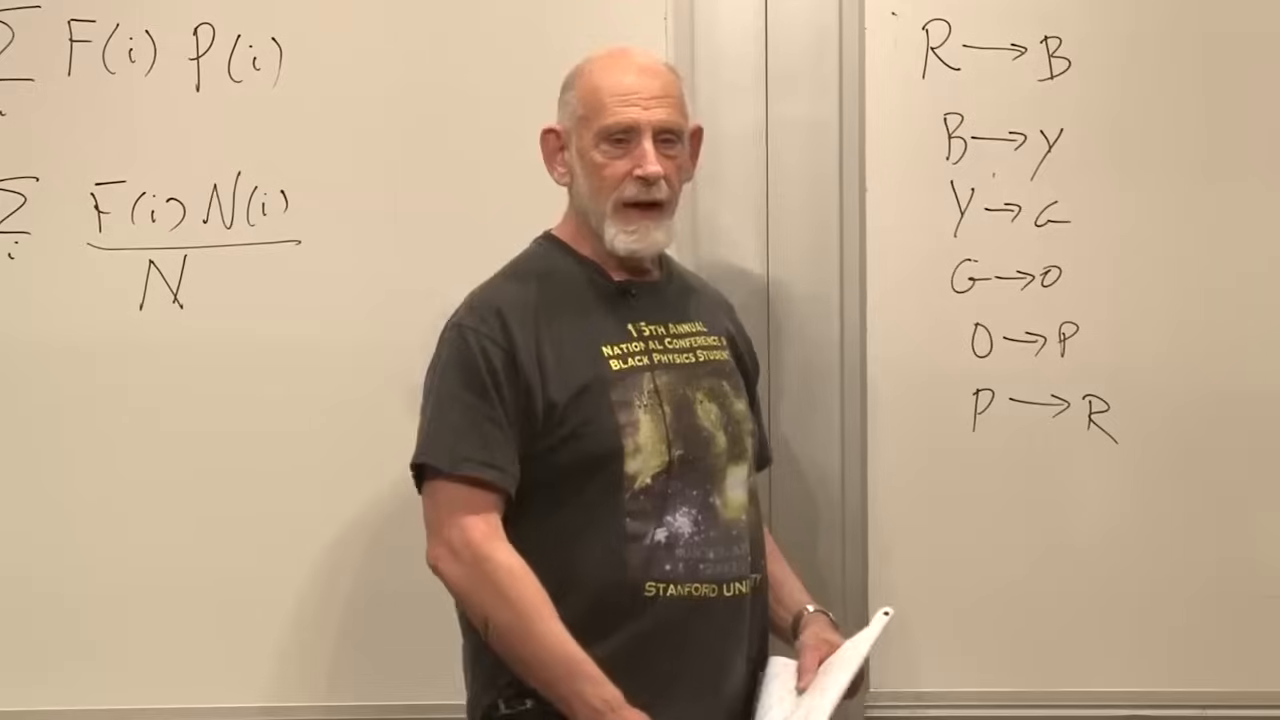
\includegraphics[width=0.92\textwidth]{lecture_01_figure_02.png}
\caption{Các công thức giá trị kỳ vọng vẫn ở bảng bên trái, còn sáu cập nhật màu tất định được liệt kê ở bên phải.}
\lectureframe{00:26:28}
\end{figure}

Danh sách trên bảng dễ hiểu hơn khi được vẽ thành một chu trình có hướng:
\begin{figure}[htbp]
\centering
\begin{tikzpicture}[
  >=Latex,
  state/.style={draw,circle,minimum size=8mm,inner sep=1pt}
]
\node[state] (R) at (90:2.2) {$R$};
\node[state] (B) at (30:2.2) {$B$};
\node[state] (Y) at (-30:2.2) {$Y$};
\node[state] (G) at (-90:2.2) {$G$};
\node[state] (O) at (-150:2.2) {$O$};
\node[state] (P) at (150:2.2) {$P$};
\draw[->] (R) -- (B);
\draw[->] (B) -- (Y);
\draw[->] (Y) -- (G);
\draw[->] (G) -- (O);
\draw[->] (O) -- (P);
\draw[->] (P) -- (R);
\end{tikzpicture}
\caption{Một quỹ đạo duy nhất gồm sáu trạng thái. Mỗi trạng thái được đi qua đúng một lần trong mỗi chu kỳ.}
\label{fig:sm1-six-cycle}
\end{figure}

Giả sử ta không biết trạng thái ban đầu và chụp một ảnh tức thời vào một thời điểm không biết. Vì mỗi bước kéo dài như nhau, hệ ở mỗi màu trong một phần sáu của chu kỳ:
\begin{equation}
 p(R)=p(B)=p(Y)=p(G)=p(O)=p(P)=\frac16.
 \label{eq:sm1-uniform-cycle}
\end{equation}
Sự bằng nhau này không đến từ hình dạng của vật. Nó đến từ việc thời gian hệ ở trong các trạng thái là như nhau.

Ta có thể sắp xếp lại các mũi tên và thu được một định luật vi mô khác mà vẫn tạo thành một chu trình gồm sáu trạng thái. Trình tự chi tiết thay đổi, nhưng xác suất của ảnh chụp tức thời vẫn là \(1/6\) vì mỗi trạng thái vẫn xuất hiện đúng một lần trong mỗi chu kỳ. Do đó, dự đoán này không cần biết điểm khởi đầu cũng không cần thứ tự chi tiết. Nó chỉ đòi hỏi cấu trúc quỹ đạo và thời gian bằng nhau cho mỗi lần cập nhật.

\begin{classroomqa}
\classquestion{Nếu vật không đối xứng, thì theo nghĩa nào việc gán cho mỗi màu xác suất \(1/6\) là hợp lệ?}
\lecturerresponse{Cách gán này mang tính động lực học chứ không phải hình học. Một ảnh chụp được lấy ở một pha chưa biết của một quỹ đạo sáu bước sẽ lấy mẫu sáu khoảng thời gian bằng nhau. Sự tương đương thích đáng ở đây là giữa các vị trí trên quỹ đạo, không phải giữa các mặt của vật. Nếu các thời gian lưu lại không bằng nhau, thì các xác suất cũng sẽ không bằng nhau.
\lecturetimestamp{00:27:11--00:29:49}}
\end{classroomqa}

\section{Các chu trình rời nhau và các đại lượng bảo toàn}

Một định luật tất định không nhất thiết đặt mọi trạng thái lên một quỹ đạo duy nhất. Hãy xét hai chu trình rời nhau,
\begin{equation}
 R\longrightarrow B\longrightarrow G\longrightarrow R,
 \qquad
 P\longrightarrow Y\longrightarrow O\longrightarrow P.
 \label{eq:sm1-two-cycles}
\end{equation}
Nếu ta biết rằng hệ nằm trên chu trình thứ nhất, thì
\begin{equation}
 \begin{aligned}
 p(R)=p(B)=p(G)&=\frac13,\\
 p(P)=p(Y)=p(O)&=0.
 \end{aligned}
\end{equation}
Biết rằng nó nằm trên chu trình thứ hai sẽ đảo ngược các cách gán này.

Trường hợp tổng quát hơn đòi hỏi các trọng số tiên nghiệm. Gán nhãn các chu trình là \(+1\) và \(-1\), và cho xác suất của chúng là \(p_+\) và \(p_-\), với
\begin{equation}
 p_++p_-=1.
\end{equation}
Khi đó,
\begin{align}
 p(R)=p(B)=p(G)&=\frac{p_+}{3},\\
 p(P)=p(Y)=p(O)&=\frac{p_-}{3}.
 \label{eq:sm1-sector-weights}
\end{align}
Các thừa số \(1/3\) suy ra từ chuyển động bên trong một chu trình. Các số \(p_+\) và \(p_-\) thì không. Chúng phải đến từ thông tin bổ sung, có lẽ từ một thí nghiệm khác hoặc một hệ khác chọn miền bảo toàn ban đầu.

Các nhãn \(+1\) và \(-1\) xác định một đại lượng bảo toàn: một khi hệ bắt đầu trên một chu trình, định luật cập nhật không bao giờ đưa nó sang chu trình kia. Ta có thể gọi đại lượng ấy là năng lượng, hoặc đặt cho nó một tên tạm như \emph{zilch}. Tên gọi của nó là thứ yếu. Bảo toàn có nghĩa là không gian trạng thái được chia thành các miền mà động lực học không thể vượt qua.

Các chu trình không nhất thiết phải chứa cùng một số trạng thái. Một quỹ đạo bốn trạng thái và một quỹ đạo hai trạng thái vẫn xác định hai miền bảo toàn. Khi đó, lấy mẫu theo các khoảng thời gian bằng nhau cho \(1/4\) trong miền thứ nhất và \(1/2\) trong miền thứ hai, trong mỗi trường hợp đều nhân với xác suất tiên nghiệm của miền đó. Cơ học thống kê phải trả lời hai câu hỏi tách biệt về mặt logic:
\begin{enumerate}
\item Trong một miền bảo toàn đã cho, động lực học dành bao nhiêu thời gian cho các trạng thái của nó?
\item Nên gán xác suất nào cho chính miền bảo toàn ấy?
\end{enumerate}

\begin{classroomqa}
\audiencequestion{Chúng ta có đang giả sử rằng mọi trạng thái bên trong một miền bảo toàn đều nhận cùng một xác suất không?}
\lecturerresponse{Đối với các định luật mô hình đơn giản rời rạc được trình bày ở đây, có, vì mỗi trạng thái tồn tại trong cùng một khoảng thời gian và chuyển động là tất định. Sự không biết nằm ở pha ban đầu của quỹ đạo. Một đầu dò có độ phân giải thời gian ở mức mili giây không thể phân biệt các lần cập nhật ở mức micro giây, mặc dù một ảnh chụp đủ nhanh vẫn có thể nhận diện trạng thái đã được chụp lại. Trong một hệ tổng quát hơn, các thời gian lưu lại không bằng nhau phải được tính đến một cách tường minh.
\lecturetimestamp{00:36:16--00:37:17}}
\end{classroomqa}

\begin{classroomqa}
\audiencequestion{Nếu lấy hai ảnh chụp tức thời và ảnh thứ nhất xác định một chu trình, thì ảnh thứ hai có nên xác định cùng chu trình đó không?}
\lecturerresponse{Có. Đó chính là ý nghĩa của bảo toàn. Một khi phép đo xác định giá trị của đại lượng bảo toàn, các xác suất trong tương lai có thể được điều kiện hóa theo giá trị đó, và các trạng thái trong miền kia nhận xác suất bằng không.
\lecturetimestamp{00:37:18--00:37:45}}
\end{classroomqa}

\subsection{Năng lượng được chia sẻ giữa hai hệ}

Bây giờ hãy thay nhãn trừu tượng bằng năng lượng. Một hộp cô lập là một hệ kín và có một năng lượng bảo toàn. Hai hộp cô lập có hai năng lượng được bảo toàn riêng rẽ vì chúng không tương tác. Nối chúng bằng một lối thông hẹp cho phép năng lượng chảy qua, và các năng lượng riêng rẽ có thể thay đổi trong khi tổng vẫn giữ cố định.

\begin{figure}[htbp]
\centering
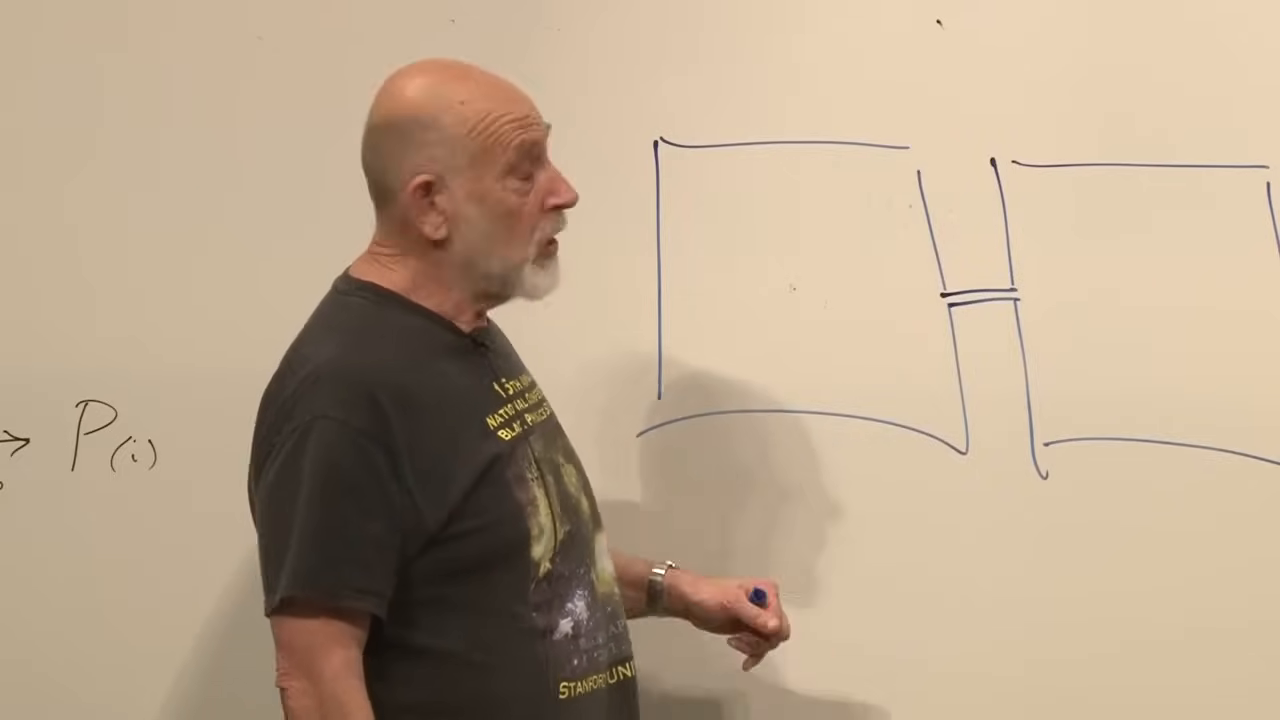
\includegraphics[width=0.92\textwidth]{lecture_01_figure_03.png}
\caption{Hai phân hệ được nối với nhau bằng một kênh hẹp mà qua đó năng lượng có thể truyền qua.}
\lectureframe{00:39:19}
\end{figure}

\begin{figure}[htbp]
\centering
\begin{tikzpicture}[>=Latex]
\draw[thick,rounded corners=4pt] (-4,1.8) rectangle (-0.7,-1.5);
\draw[thick,rounded corners=4pt] (0.7,1.5) rectangle (4,-1.8);
\draw[thick] (-0.7,0.45) -- (0.7,0.45);
\draw[thick] (-0.7,-0.35) -- (0.7,-0.35);
\draw[<->,very thick] (-0.45,0.05) -- (0.45,0.05);
\node at (-2.35,0.15) {subsystem \(1\)};
\node at (2.35,-0.15) {subsystem \(2\)};
\node[above] at (0,0.5) {energy exchange};
\end{tikzpicture}
\caption{Một khi mối nối được mở ra, chỉ còn \(E_1+E_2\) là được bảo toàn. Sự phân chia năng lượng trở thành một bài toán xác suất.}
\label{fig:sm1-connected-systems}
\end{figure}

Với một tổng năng lượng đã cho, ta có thể hỏi xác suất để phân hệ \(1\) có \(E_1\) trong khi phân hệ \(2\) có phần còn lại. Các hộp giống nhau trung bình phải có năng lượng bằng nhau, nhưng giá trị trung bình không phải là toàn bộ phân bố. Vì vậy, một cách để xác định các xác suất cho một phân hệ là đặt nó vào trong một hệ kín lớn hơn, mà định luật bảo toàn của hệ đó cung cấp thông tin còn thiếu. Cách xây dựng này sẽ còn lặp lại xuyên suốt cơ học thống kê.

\section{Các định luật tốt, các định luật xấu, và định luật âm thứ nhất}

Không phải mọi quy tắc cập nhật tất định đều có thể chấp nhận như một định luật cơ bản. Hãy xét ánh xạ
\begin{equation}
 \begin{aligned}
 R&\mapsto R,& B&\mapsto R,& Y&\mapsto R,\\
 G&\mapsto R,& O&\mapsto R,& P&\mapsto R.
 \end{aligned}
 \label{eq:sm1-all-to-red}
\end{equation}
Nó dự đoán tương lai một cách hoàn hảo: sau một bước, trạng thái là đỏ. Nó thất bại theo chiều ngược lại. Một khi hệ đã ở trạng thái đỏ, không có gì cho biết liệu nó đến từ xanh dương, vàng, xanh lục, cam, tím, hay từ chính đỏ.

\begin{figure}[htbp]
\centering
\begin{tikzpicture}[
  >=Latex,
  state/.style={draw,circle,minimum size=8mm,inner sep=1pt}
]
\node[state,fill=red!12] (R) at (0,0) {$R$};
\node[state] (B) at (-3,1.6) {$B$};
\node[state] (Y) at (-3,0) {$Y$};
\node[state] (G) at (-3,-1.6) {$G$};
\node[state] (O) at (3,1.6) {$O$};
\node[state] (P) at (3,-1.6) {$P$};
\draw[->] (B) -- (R);
\draw[->] (Y) -- (R);
\draw[->] (G) -- (R);
\draw[->] (O) -- (R);
\draw[->] (P) -- (R);
\draw[->,loop above] (R) to (R);
\end{tikzpicture}
\caption{Một định luật nhiều-đến-một dự đoán trạng thái kế tiếp nhưng xóa bỏ sự phân biệt giữa các trạng thái quá khứ khả dĩ.}
\label{fig:sm1-bad-law}
\end{figure}

Ngược lại, một chu trình kín bảo toàn dấu vết. Nếu biết thời gian đã trôi qua, ta có thể tiến hóa trạng thái theo chiều tiến hoặc chiều lùi, ngay cả sau nhiều nghìn chu kỳ. Định luật bảo toàn sự phân biệt giữa các điều kiện ban đầu. Susskind gọi yêu cầu này là \emph{định luật âm thứ nhất của vật lý}: thông tin không bị mất đi một cách căn bản.

Đối với một không gian trạng thái rời rạc hữu hạn, tiêu chuẩn bằng sơ đồ rất đơn giản:
\begin{quote}
Mỗi trạng thái của một định luật tốt có đúng một mũi tên đi ra và đúng một mũi tên đi vào.
\end{quote}
Mũi tên đi ra xác định tương lai; mũi tên đi vào tái dựng quá khứ. Về mặt toán học, phép cập nhật là một hoán vị của các trạng thái.

\subsection{Ma sát chỉ là một phản ví dụ biểu kiến}

Đối ứng liên tục là định lý Liouville. Ma sát dường như mâu thuẫn với nó. Hãy cho một cục tẩy trượt trên mặt bàn; dù nó bắt đầu ở đâu, cuối cùng nó cũng sẽ dừng lại. Một phương trình lực cản mang tính sơ đồ là
\begin{equation}
 m\ddot x=-\gamma\dot x,
 \qquad \gamma>0.
 \label{eq:sm1-drag}
\end{equation}
Vận tốc của nó suy giảm theo hàm mũ. Nếu đây là định luật nền tảng tối hậu của mọi hạt trong một căn phòng kín, thì mọi chuyển động đều sẽ tắt hẳn, nhiệt độ sẽ giảm về không, và nhiều trạng thái ban đầu sẽ sụp vào một trạng thái cuối cùng. Bảo toàn năng lượng sẽ không còn đúng, thông tin sẽ biến mất, và độ hỗn độn sẽ giảm đi. Đây sẽ là phiên bản liên tục của việc mọi thứ đều đi tới đỏ.

Ma sát thực không làm như vậy. Cục tẩy làm nóng mặt bàn, chính nó và môi trường xung quanh. Các vị trí và động lượng vi mô lưu lại những khác biệt đã mất khỏi chuyển động nhìn thấy được. Ma sát là một phương trình hiệu dụng cho một phân hệ sau khi đã lược bỏ các bậc tự do không quan sát được; nó không phải là một định luật tiêu tán cơ bản cho toàn bộ hệ kín.

\begin{classroomqa}
\classquestion{Phương trình vi phân \(m\ddot x=-\gamma\dot x\) biểu diễn điều gì, và vì sao nó không phải là một định luật cơ bản cho hệ kín?}
\lecturerresponse{Nó biểu diễn lực cản nhớt. Tự nó, nó kéo mọi vận tốc về không, điều đó sẽ làm cho một chất khí nguội xuống về không bất kể nhiệt độ ban đầu của nó. Trong một mô tả kín thực sự, năng lượng cơ học và thông tin bị mất sẽ chuyển vào các bậc tự do vi mô. Phương trình lực cản chỉ đáng tin cậy sau khi các biến đó đã được lược bỏ.
\lecturetimestamp{00:44:40--00:48:56}}
\end{classroomqa}

\section{Các trạng thái được chiếm và entropy đầu tiên}

Bảo toàn thông tin có một phát biểu xác suất tương đương. Giả sử \(M\) trong số \(N\) trạng thái được gán xác suất bằng nhau,
\begin{equation}
 p_i=
 \begin{cases}
 1/M, & i\text{ in the occupied set},\\
 0, & i\text{ outside it}.
 \end{cases}
 \label{eq:sm1-uniform-occupied}
\end{equation}
Một phép cập nhật bảo toàn thông tin có thể xáo lại những trạng thái nào được chiếm, nhưng nó không thể gộp chúng lại. Ở mọi thời điểm về sau vẫn còn \(M\) trạng thái, mỗi trạng thái có xác suất \(1/M\). Trái lại, ánh xạ xấu \eqref{eq:sm1-all-to-red} có thể làm nhiều trạng thái được chiếm sụp vào một trạng thái duy nhất.

Số \(M\) đo mức độ không biết của ta. Nếu \(M=N\), mọi trạng thái đều có thể và sự không biết của ta là cực đại. Nếu \(M=1\), trạng thái vi mô được biết chính xác. Vì thế định nghĩa đầu tiên của entropy là
\begin{equation}
 S=\log M.
 \label{eq:sm1-entropy-logm}
\end{equation}
Nó cho
\begin{equation}
 S_{\max}=\log N,
 \qquad
 S_{\min}=0.
\end{equation}
Nếu không gian trạng thái là vô hạn, thì có thể không tồn tại cận trên hữu hạn.

Trong cách phát triển này, entropy xuất hiện trước nhiệt độ, và thậm chí còn trước cả phát biểu hình thức của bảo toàn năng lượng. Theo nghĩa đó, nó cơ bản hơn. Tuy vậy, nó không phải chỉ là một tính chất của riêng hệ cơ học. Nó đồng thời phụ thuộc vào hệ và vào phân bố xác suất biểu diễn điều đã biết. Cùng một hệ cơ học có thể được những người quan sát có thông tin khác nhau gán các entropy khác nhau.

Dưới sự tiến hóa vi mô chính xác, các trạng thái được chiếm chỉ bị sắp xếp lại, nên entropy phân giải mịn này được bảo toàn. Trên thực tế, ta mất thông tin về thời điểm, bỏ qua các tương quan, và không thể theo dõi số lượng khổng lồ các biến. Khi đó phân bố xác suất của ta trải ra trên nhiều khả năng hơn, và entropy gán cho mô tả thô tăng lên. Các phương trình không nhất thiết phải hủy thông tin thì mô tả mà ta có thể sử dụng mới mất đi thông tin.

\begin{classroomqa}
\classquestion{Entropy lớn nhất có thể có của một hệ hữu hạn với \(N\) trạng thái là bao nhiêu?}
\lecturerresponse{Đó là \(\log N\), đạt được khi tất cả \(N\) trạng thái đều có xác suất như nhau. Entropy nhỏ nhất là 0, đạt được khi một trạng thái có xác suất bằng 1. Vì vậy entropy đo cả trạng thái hiểu biết lẫn không gian trạng thái khả dụng.
\lecturetimestamp{00:56:46--00:58:19}}
\end{classroomqa}

\section{Dòng Liouville trong không gian pha liên tục}

Đối với các hạt có vị trí và động lượng liên tục, một trạng thái vi mô là một điểm trong không gian pha. Ta ký hiệu các tọa độ là \(q_a\) và các động lượng liên hợp của chúng là \(p_a\). Với nhiều hạt thì có cực kỳ nhiều trục; một hình vẽ hai chiều với một \(q\) và một \(p\) chỉ là hình minh họa thay thế. Không gian pha có số chiều chẵn vì mỗi tọa độ đều có một động lượng đi kèm.

Giả sử tri thức của ta được biểu diễn bởi một miền \(\Omega_0\): mật độ xác suất đồng đều bên trong miền và bằng 0 ở bên ngoài. Chẳng hạn, biết rằng mọi hạt đều nằm trong phòng sẽ giới hạn các tọa độ vị trí, còn các cận về tốc độ của chúng sẽ giới hạn các tọa độ động lượng.

Sự tiến hóa Hamilton đưa mỗi điểm của không gian pha dọc theo một quỹ đạo. Các điểm lân cận chuyển tới các điểm lân cận, và vùng bị chiếm chảy như một khối chất lỏng không nén được:
\begin{figure}[htbp]
\centering
\begin{tikzpicture}[>=Latex,scale=0.95]
\draw[->] (-4.2,0) -- (4.3,0) node[right] {$q$};
\draw[->] (-3.7,-2.2) -- (-3.7,2.4) node[above] {$p$};
\draw[fill=blue!12,thick]
  (-3.0,-0.5) .. controls (-2.7,1.0) and (-1.3,1.2) .. (-0.9,0.1)
  .. controls (-0.6,-1.0) and (-2.2,-1.4) .. cycle;
\node at (-1.9,0.0) {$\Omega_0$};
\draw[->,very thick] (-0.3,0.2) -- (0.8,0.2);
\draw[fill=orange!15,thick]
  (1.2,-1.1) .. controls (1.5,0.3) and (2.3,1.8) .. (3.2,1.1)
  .. controls (3.6,0.7) and (2.8,-0.4) .. (2.5,-1.5)
  .. controls (2.1,-1.8) and (1.5,-1.6) .. cycle;
\node at (2.35,0.1) {$\Omega_t$};
\end{tikzpicture}
\caption{Dòng Hamilton có thể kéo giãn và cắt trượt một vùng không gian pha bị chiếm, nhưng vẫn bảo toàn thể tích của nó.}
\label{fig:sm1-liouville-flow}
\end{figure}

Định lý Liouville phát biểu rằng
\begin{equation}
 \operatorname{Vol}(\Omega_t)
 =
 \operatorname{Vol}(\Omega_0).
 \label{eq:sm1-liouville-volume}
\end{equation}
Nếu mật độ ban đầu đồng đều trên \(\Omega_0\), thì sau khi tiến hóa nó vẫn đồng đều trên \(\Omega_t\). Đây là tương tự liên tục của việc bảo toàn số lượng và trọng số của các trạng thái rời rạc được chiếm.

Định lý này cũng giải quyết bài toán ma sát theo cách hình học. Nếu chỉ nhìn vào động lượng nhìn thấy được của cục tẩy, một đám mây các khả năng dường như bị ép về phía \(p=0\). Trong không gian pha đầy đủ, đám mây ấy lan sang các vị trí và động lượng của các phân tử trong cục tẩy và mặt bàn. Một phép chiếu có thể co lại trong khi toàn bộ thể tích nhiều chiều vẫn không đổi.

\begin{classroomqa}
\classquestion{Nếu mọi quỹ đạo nhìn thấy được đều tiến tới trạng thái nghỉ, thì vùng không gian pha bị chiếm có sụp xuống trục \(p=0\) hay không?}
\lecturerresponse{Chỉ trong phép chiếu rút gọn. Hệ đầy đủ chứa các biến vi mô của mặt bàn, cục tẩy và môi trường xung quanh. Khi khoảng động lượng nhìn thấy được thu hẹp lại, phân bố lan ra theo những hướng ẩn đó. Định lý Liouville áp dụng cho toàn bộ không gian pha kín đầy đủ, chứ không áp dụng cho một tập biến vĩ mô không đầy đủ.
\lecturetimestamp{01:04:37--01:06:29}}
\end{classroomqa}

\section{Từ định luật âm một đến định luật thứ nhất}

\subsection{Một cái nhìn ngắn gọn về định luật thứ không}

Trước khi phát biểu định luật thứ nhất, sẽ hữu ích nếu nhắc đến định luật thứ không. Cân bằng nhiệt vẫn chưa được định nghĩa, nên lúc này định luật ấy chỉ là một phát biểu về cấu trúc:
\begin{quote}
Nếu hệ \(A\) cân bằng nhiệt với \(B\), và \(B\) cân bằng nhiệt với \(C\), thì \(A\) cân bằng nhiệt với \(C\).
\end{quote}
Tính bắc cầu này về sau sẽ cho phép định nghĩa nhiệt độ. Còn lúc này, ta tạm gác nó sang một bên.

\subsection{Bảo toàn năng lượng}

Định luật thứ nhất đối với một hệ kín đơn giản là
\begin{equation}
 \frac{dE}{dt}=0.
 \label{eq:sm1-first-law}
\end{equation}
Dạng súc tích của nó che khuất sức mạnh của nó. Năng lượng là một đại lượng bảo toàn, và từ năng lượng về sau sẽ mang nội dung nhiệt động lực học phong phú hơn.

Nếu một hệ kín gồm hai phần và năng lượng của chúng là cộng tính,
\begin{equation}
 E=E_1+E_2,
\end{equation}
thì
\begin{equation}
 \frac{dE_1}{dt}+\frac{dE_2}{dt}=0,
 \qquad\text{or}\qquad
 \frac{dE_1}{dt}=-\frac{dE_2}{dt}.
 \label{eq:sm1-energy-exchange}
\end{equation}
Dạng thứ hai làm cho sự trao đổi trở nên tường minh: năng lượng mà một hệ con mất đi chính là năng lượng mà hệ con kia nhận được.

Giả thiết cộng tính đòi hỏi phải cẩn thận. Hai hạt hấp dẫn nhau có các động năng riêng lẻ, nhưng tương tác của chúng đóng góp một thế năng thuộc về cả cặp. Tổng năng lượng vẫn được bảo toàn dù nó không thể được viết chính xác thành năng lượng của vật này cộng với năng lượng của vật kia.

Trong nhiệt động lực học, ta thường có thể dùng một xấp xỉ cộng tính rất tốt vì năng lượng khối tỉ lệ theo thể tích, trong khi năng lượng tương tác tầm ngắn giữa các phần lớn kề nhau chủ yếu tỉ lệ theo diện tích tiếp xúc của chúng. Hãy chia một cái bàn lớn thành các khối: nội năng của mỗi khối là một hiệu ứng thể tích, còn sự ghép giữa các khối kề nhau là một hiệu ứng bề mặt. Với các khối lớn, hiệu ứng sau nhỏ hơn một cách tương đối. Phương trình \eqref{eq:sm1-first-law} là chính xác cho toàn bộ hệ kín; dạng cho hệ con \eqref{eq:sm1-energy-exchange} giả sử năng lượng tương tác có thể bỏ qua.

\begin{classroomqa}
\audiencequestion{Điều kiện chuẩn hóa \(\sum_i p_i=1\) có đồng thời giả thiết rằng các kết quả được liệt kê loại trừ lẫn nhau hay không?}
\lecturerresponse{Có. Một nhãn trạng thái được định nghĩa sao cho các khả năng không chồng lấn lên nhau: nếu con xúc xắc ở trạng thái màu vàng, thì đồng thời nó không ở trạng thái màu đỏ. Trong ngôn ngữ thông thường các màu có thể được pha trộn, nhưng phân hoạch trạng thái dùng trong phép tính xác suất phải gồm các khả năng loại trừ lẫn nhau.
\lecturetimestamp{01:12:14--01:12:55}}
\end{classroomqa}

\section{Quay trở lại entropy}

Bài giảng giờ đây quay lại một cách tường minh với những điểm còn dang dở. Nhiệt độ, dù quen thuộc với giác quan, là một đại lượng dẫn xuất. Entropy và năng lượng phải được thiết lập trước thì mới có thể định nghĩa nhiệt độ một cách rành mạch.

\subsection{Các phân bố xác suất tổng quát}

Định nghĩa đặc biệt \(S=\log M\) áp dụng khi \(M\) trạng thái có xác suất bằng nhau và mọi trạng thái khác có xác suất bằng 0. Một phân bố tổng quát không nhất thiết phải có dạng hình chữ nhật. Các trọng số của nó có thể biến thiên trơn tru hoặc bất quy tắc theo các nhãn trạng thái.

\begin{figure}[htbp]
\centering
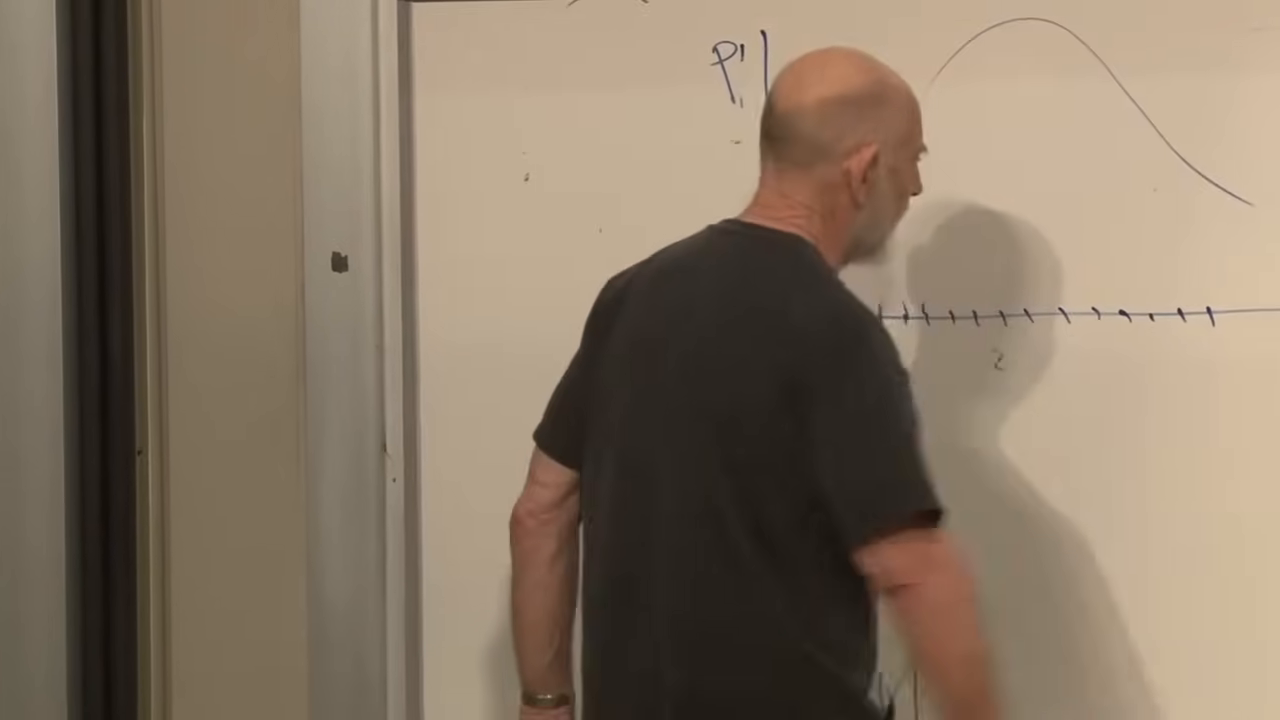
\includegraphics[width=0.92\textwidth]{lecture_01_figure_05.png}
\caption{Một phân bố xác suất được vẽ trên các nhãn trạng thái rời rạc. Điều cần cho entropy là độ trải rộng, chứ không phải chính xác hình dạng của đường cong.}
\lectureframe{01:14:40}
\end{figure}

\begin{figure}[htbp]
\centering
\resizebox{\linewidth}{!}{%
\begin{tikzpicture}[>=Latex,scale=0.93]
\draw[->] (-4.2,0) -- (4.4,0) node[right] {state label \(i\)};
\draw[->] (-4,0) -- (-4,3.2) node[above] {$p_i$};
\foreach \x in {-3.6,-3.1,...,3.6}
  \draw (\x,0.08) -- (\x,-0.08);
\draw[very thick]
  plot[smooth] coordinates {
  (-3.7,0.12) (-3.0,0.28) (-2.3,0.72) (-1.6,1.45)
  (-0.9,2.25) (-0.2,2.65) (0.5,2.28) (1.2,1.55)
  (1.9,0.88) (2.7,0.38) (3.5,0.14)};
\draw (-1.8,-0.18) -- (-1.8,-0.5);
\draw (1.8,-0.18) -- (1.8,-0.5);
\draw[<->] (-1.8,-0.46) -- (1.8,-0.46);
\node at (0,-0.82) {effective spread};
\end{tikzpicture}
}
\caption{Một phân bố hẹp mang ít bất định hơn một phân bố rộng. Entropy phải đo toàn bộ phân bố.}
\label{fig:sm1-probability-spread}
\end{figure}

Định nghĩa tổng quát là
\begin{equation}
 S=-\sum_i p_i\log p_i.
 \label{eq:sm1-shannon-entropy}
\end{equation}
Dùng \eqref{eq:sm1-expectation}, ta được
\begin{equation}
 S=-\langle\log p\rangle.
\end{equation}
Dấu trừ bù cho thực tế rằng \(\log p_i<0\) khi \(0<p_i<1\).

\subsection{Khôi phục kết quả của phân bố đồng đều}

Ta phải kiểm tra rằng công thức tổng quát tái tạo lại định nghĩa đầu tiên. Đối với một trạng thái không được chiếm, \(p_i=0\) còn \(\log p_i\) phân kỳ. Tích đó có giá trị giới hạn xác định rõ
\begin{equation}
 \lim_{p\to0^+}p\log p=0.
 \label{eq:sm1-plogp-limit}
\end{equation}
Vì thế các trạng thái có xác suất bằng 0 không đóng góp gì.

\begin{classroomqa}
\audiencequestion{Nếu \(p_i=0\), thì số hạng đó có thực sự bằng không không? Logarit của số không là âm vô cực.}
\lecturerresponse{Số hạng này được định nghĩa bởi giới hạn \(\lim_{p\to0^+}p\log p\), và giới hạn đó bằng không. Thừa số \(p\) tiến về không nhanh hơn logarit phân kỳ. Do đó, các trạng thái có xác suất nhỏ đến mức tùy ý cho những đóng góp nhỏ đến mức tùy ý, còn một trạng thái hoàn toàn không thể xảy ra thì không đóng góp gì.
\lecturetimestamp{01:18:27--01:19:46}}
\end{classroomqa}

Đối với mỗi trạng thái trong \(M\) trạng thái được chiếm, \(p_i=1/M\). Do đó
\begin{align}
 S
 &=-\sum_{\mathrm{occupied}\ i}
 \frac1M\log\!\left(\frac1M\right)\\
 &=-M\frac1M\log\!\left(\frac1M\right)\\
 &=-\log\!\left(\frac1M\right)
 =\log M.
 \label{eq:sm1-entropy-check}
\end{align}
Biểu thức tổng quát khớp chính xác với biểu thức đặc biệt. Một phân bố rộng hơn đặt trọng số đáng kể lên nhiều khả năng hơn nên có entropy lớn hơn; một phân bố hẹp hơn có entropy nhỏ hơn.

\begin{figure}[htbp]
\centering
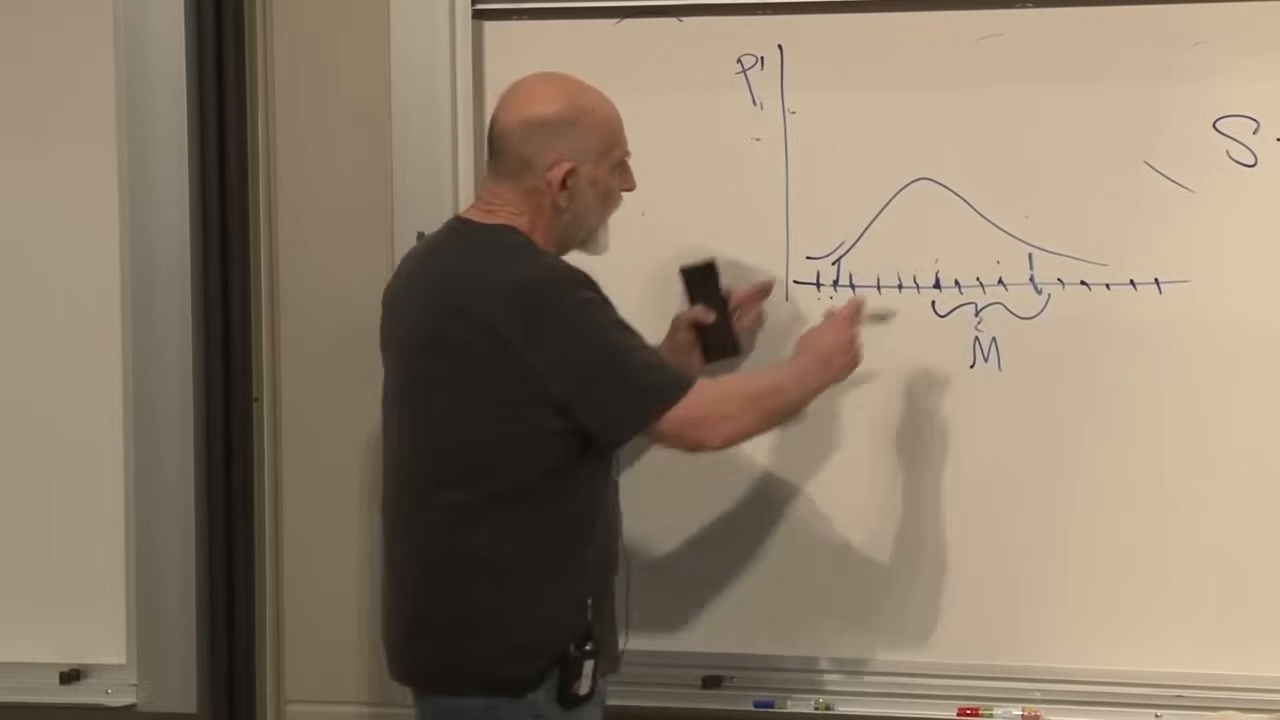
\includegraphics[width=0.92\textwidth]{lecture_01_figure_06.png}
\caption{Độ rộng được đánh dấu \(M\) nhấn mạnh mối liên hệ giữa độ trải của các xác suất đáng kể và entropy.}
\lectureframe{01:16:42}
\end{figure}

Entropy thuộc về một phân bố xác suất trên không gian trạng thái. Nó không phải là một đại lượng quan sát thuần túy như năng lượng hay động lượng của một vi trạng thái. Một trạng thái chính xác có thể được biểu diễn bằng một phân bố tập trung tại trạng thái đó và khi ấy có entropy bằng 0, nhưng entropy thay đổi khi trạng thái hiểu biết thay đổi.

\section{Đồng xu, bit và phép đếm tường minh}

Gọi \(n\) là số đồng xu. Số cấu hình vi mô là
\begin{equation}
 N=2^n.
 \label{eq:sm1-coin-state-count}
\end{equation}
Nếu không biết gì về các đồng xu, thì tất cả \(2^n\) cấu hình đều có xác suất như nhau, và
\begin{equation}
 S_{\max}=\log(2^n)=n\log2.
 \label{eq:sm1-coin-max-entropy}
\end{equation}
Entropy là cộng tính theo số đồng xu độc lập.

Với logarit cơ số \(2\), một hệ hai trạng thái hoàn toàn chưa biết có entropy bằng 1 bit. Với logarit tự nhiên, nó có entropy bằng \(\log2\). Đơn vị là quy ước; thứ tự và tính cộng tính cơ bản không đổi.

Ở cực kia, nếu mọi đồng xu đều đã biết, thì chính xác một cấu hình có xác suất bằng 1:
\begin{equation}
 S=0.
\end{equation}
Biết nhiều hơn nghĩa là entropy ít hơn.

Bây giờ giả sử chính xác một trong \(n\) đồng xu là sấp, còn tất cả các đồng xu khác đều ngửa, và vị trí của mặt sấp là chưa biết. Có \(n\) cấu hình có khả năng như nhau, mỗi cấu hình ứng với một vị trí khả dĩ của mặt sấp, nên
\begin{equation}
 S=\log n.
 \label{eq:sm1-one-tail-entropy}
\end{equation}
Nói chung đây không phải là bội số nguyên của \(\log2\). Bit là một đơn vị tiện lợi, chứ không phải khẳng định rằng mọi entropy đều xuất hiện theo các bậc nguyên bit.

\begin{classroomqa}
\audiencequestion{Có phải \(\log2\) chỉ xuất hiện vì mỗi đồng xu có hai trạng thái khả dĩ? Một phần tử có ba trạng thái thì sẽ cho \(\log3\) chứ?}
\lecturerresponse{Chính xác. Một phần tử hoàn toàn chưa biết với \(k\) trạng thái khả dĩ đóng góp \(\log k\). Các công tắc nhị phân đặc biệt thuận tiện trong máy tính vì các công tắc vật lý tự nhiên hiện thực hóa hai trạng thái ổn định và vì hai là số nguyên nhỏ nhất không tầm thường.
\lecturetimestamp{01:29:55--01:30:48}}
\end{classroomqa}

\begin{classroomqa}
\audiencequestion{Logarit ở đây được hiểu theo cơ số nào?}
\lecturerresponse{Trong các công thức vật lý này, \(\log\) có nghĩa là logarit tự nhiên. Các nhà lý thuyết thông tin thường dùng cơ số \(2\), nên entropy được đo trực tiếp bằng bit. Thay đổi cơ số chỉ nhân mọi entropy với cùng một hệ số chuyển đổi cố định và không làm thay đổi kết luận vật lý nào.
\lecturetimestamp{01:30:49--01:32:06}}
\end{classroomqa}

\section{Entropy trong không gian pha liên tục}

Quay lại không gian pha cổ điển \(\Gamma\). Nếu mật độ xác suất là đều trên một miền có thể tích \(V_\Gamma\) và bằng 0 ở bên ngoài, thì tương tự với việc đếm \(M\) trạng thái đồng khả năng là
\begin{equation}
 S=\log\!\left(\frac{V_\Gamma}{V_0}\right).
 \label{eq:sm1-continuous-uniform}
\end{equation}
Ở đây \(V_\Gamma\) là thể tích trong toàn bộ không gian nhiều chiều của các tọa độ và xung lượng, không phải thể tích không gian thông thường. Thể tích cố định \(V_0\) là một ô tham chiếu của không gian pha, làm cho logarit trở thành vô thứ nguyên. Đặt \(V_0=1\) thì cho cách viết tắt \(S=\log V_\Gamma\) được dùng trên bảng.

Đối với một mật độ xác suất tổng quát \(P(q,p)\), tổng rời rạc trở thành một tích phân trên không gian pha. Điều kiện chuẩn hóa là
\begin{equation}
 \int_\Gamma d\Gamma\,P(q,p)=1,
 \label{eq:sm1-continuous-normalization}
\end{equation}
và entropy là
\begin{equation}
 S=-\int_\Gamma d\Gamma\,
 P(q,p)\log\!\bigl[P(q,p)V_0\bigr].
 \label{eq:sm1-continuous-entropy}
\end{equation}
Mật độ là xác suất trên mỗi ô không gian pha. Về mặt khái niệm,
\eqref{eq:sm1-continuous-entropy} vẫn đo mức độ phân bố rộng của xác suất; đối với một vùng phân bố đều, nó thu về logarit của thể tích bị chiếm, đo theo đơn vị của ô tham chiếu. Thay đổi ô cố định đó làm tịnh tiến mọi entropy liên tục cùng một hằng số cộng và giữ nguyên các hiệu entropy.

\begin{classroomqa}
\audiencequestion{Vì sao ký hiệu tọa độ lại đổi từ \(x\) sang \(q\)?}
\lecturerresponse{Không có thay đổi vật lý nào. Cơ học cổ điển thường dùng hoặc \(x\) hoặc \(q\) cho các tọa độ và \(p\) cho các xung lượng liên hợp. Việc đổi ký hiệu chỉ là một sơ suất; cách xây dựng không gian pha là như nhau.
\lecturetimestamp{01:37:10--01:37:39}}
\end{classroomqa}

Nhiệt độ và phân bố Boltzmann được cố ý để lại sau. Nhiệm vụ tiếp theo sẽ là định nghĩa cân bằng nhiệt rồi xác định phân bố xác suất tương ứng.

\section{Các câu hỏi về tương quan, tính cộng và thông tin}

\subsection{Tương quan nghĩa là một phép đo làm thay đổi một phân bố khác}

Sự không biết gì hoàn toàn về các đồng xu độc lập gán xác suất bằng nhau cho mọi cấu hình. Khi đó, đo một đồng xu không cho ta biết gì về bất kỳ đồng xu nào khác. Các phân bố của chúng không thay đổi.

Ensemble có đúng một mặt sấp thì khác. Nếu đồng xu được đo ra mặt sấp, thì mọi đồng còn lại chắc chắn là mặt ngửa. Nếu đồng xu được đo ra mặt ngửa, thì mặt sấp duy nhất phải nằm trong \(n-1\) đồng còn lại, nên mỗi vị trí còn lại có xác suất có điều kiện
\begin{equation}
\begin{aligned}
 p(&\text{tail at a specified remaining position}\\
   &\mid\text{measured head})=\frac{1}{n-1}.
\end{aligned}
 \label{eq:sm1-conditional-tail}
\end{equation}
Đây là tương quan: biết một biến làm thay đổi phân bố xác suất được gán cho một biến khác.

\begin{classroomqa}
\audiencequestion{Trong các ví dụ về entropy có giả thiết các đồng xu độc lập với nhau không?}
\lecturerresponse{Chỉ khi sự không biết gì hoàn toàn được biểu diễn bằng các xác suất bằng nhau cho toàn bộ \(2^n\) cấu hình. Trong trường hợp đó, đo một đồng xu không làm thay đổi các phân bố của những đồng khác. Ví dụ một-mặt-sấp là trường hợp có tương quan tường minh: một phép đo cập nhật điều gì còn có thể xảy ra ở nơi khác. Thông tin đã nêu quyết định phân bố xác suất nào đang được dùng.
\lecturetimestamp{01:38:43--01:41:58}}
\end{classroomqa}

Ví dụ các chu trình rời nhau có cùng dạng lôgic. Việc đo nhãn được bảo toàn \(+1\) hoặc \(-1\) giới hạn mọi trạng thái về sau vào một phân khu. Điều kiện hóa theo thông tin được bảo toàn làm thay đổi phân bố được phép.

Entropy có tính cộng đối với các hệ không tương quan. Nếu
\begin{equation}
 p_{ij}=p_i^{(A)}p_j^{(B)},
\end{equation}
thì
\begin{align}
 S_{AB}
 &=-\sum_{i,j}p_i^{(A)}p_j^{(B)}
 \log\!\left[p_i^{(A)}p_j^{(B)}\right]\\
 &=S_A+S_B.
 \label{eq:sm1-entropy-additivity}
\end{align}
Các tương quan ngăn cản sự phân tích nhân tử này và làm giảm độ bất định độc lập của cả cặp.

Như một bài tập, hãy hình dung một hàng các biến nhị phân mà trong đó một trạng thái lên khiến mỗi láng giềng có xác suất ba phần tư ở trạng thái xuống. Đo một vị trí ngay lập tức làm thay đổi điều ta biết về các vị trí lân cận. Một phân bố như vậy là có tương quan, và entropy của nó không thể được tìm bằng cách cộng các entropy một-vị-trí cô lập mà không tính đến các tương quan đó.

\subsection{Boltzmann, Shannon và độ bất định lượng tử}

\begin{classroomqa}
\audiencequestion{Entropy nhiệt động học ra đời sớm hơn liên hệ thế nào với entropy lý thuyết thông tin của Shannon?}
\lecturerresponse{Cùng một dạng hàm xuất hiện trong cả hai:
\(-\sum_i p_i\log p_i\). Shannon thường dùng cơ số \(2\), còn các nhà vật lý thường dùng logarit tự nhiên và khôi phục hằng số Boltzmann khi entropy được biểu diễn theo đơn vị nhiệt động học. Khác biệt về mặt toán học chỉ là một hệ số chuyển đổi cố định, mặc dù các câu hỏi vật lý dùng để xác định các xác suất có thể rất khác nhau.
\lecturetimestamp{01:44:05--01:46:06}}
\end{classroomqa}

Đối với các vi trạng thái đồng khả năng, công thức nhiệt động học thường được viết
\begin{equation}
 S_{\mathrm{thermo}}=k_{\mathrm B}\log W,
 \label{eq:sm1-boltzmann-formula}
\end{equation}
trong đó \(W\) là số vi trạng thái khả dĩ có thể tiếp cận. Trong hệ đơn vị với \(k_{\mathrm B}=1\), đây chính xác là \(S=\log W\). Hằng số Boltzmann chuyển đổi giữa đơn vị nhiệt độ và đơn vị năng lượng; thang vi mô tự nhiên của nhiệt độ là năng lượng.

\begin{classroomqa}
\audiencequestion{Entropy này có đơn thuần chỉ là một dạng khác của nguyên lý bất định Heisenberg không?}
\lecturerresponse{Không. Entropy đang xét đo độ bất định trong một phân bố xác suất trên các trạng thái khả dĩ. Trong ngôn ngữ lượng tử, đó là độ bất định của một trạng thái hỗn hợp, không phải độ bất định nội tại của phép đo, vốn vẫn có thể còn tồn tại ngay cả đối với một trạng thái thuần. Cần giữ tách biệt hai khái niệm này.
\lecturetimestamp{01:46:07--01:47:31}}
\end{classroomqa}

\section{Những điều đã được thiết lập}

Điểm xuất phát không phải là tính ngẫu nhiên trong các định luật. Động lực học tất định, kết hợp với sự hiểu biết không đầy đủ về trạng thái ban đầu, đã tạo ra các xác suất. Một quỹ đạo đơn gán các trọng số thông qua thời gian lưu ở mỗi trạng thái; các quỹ đạo rời nhau bộc lộ các đại lượng bảo toàn và đòi hỏi các trọng số tiên nghiệm giữa các phân khu. Các định luật vi mô được chấp nhận bảo toàn các phân biệt; trong không gian trạng thái hữu hạn, điều đó có nghĩa là ở mỗi trạng thái có một mũi tên đi vào và một mũi tên đi ra, còn trong cơ học liên tục thì trở thành định lý Liouville.

Cấu trúc đó trước hết dẫn tới
\begin{equation}
 S=\log M
\end{equation}
cho \(M\) trạng thái được chiếm có xác suất bằng nhau, rồi tới
\begin{equation}
 S=-\sum_i p_i\log p_i,
\end{equation}
và cuối cùng tới tích phân trên không gian pha của nó. Entropy ghi nhận một phân bố xác suất và vì thế phản ánh một trạng thái hiểu biết. Thông tin hạt mịn được định luật vi mô bảo toàn ngay cả khi một mô tả thô hạt, mang tính thực dụng, không còn theo dõi được nó.

Bảo toàn năng lượng cho ta định luật thứ nhất, còn tính cộng của năng lượng các hệ con đòi hỏi năng lượng tương tác có thể bỏ qua. Entropy có tính cộng dưới một điều kiện tương ứng: các xác suất của các hệ con phải không tương quan. Hai kiểu tính cộng này chuẩn bị cho bước tiếp theo, nơi cân bằng nhiệt, nhiệt độ và phân bố Boltzmann sẽ nối năng lượng với xác suất.

\chapter{Nhiệt độ từ entropy và năng lượng}

\lectureoverview{Ban đầu, nhiệt độ xuất hiện như một phép chuyển đổi từ các đơn vị nhiệt kế của con người sang các đơn vị năng lượng vi mô. Sau khi thực hiện phép chuyển đổi tương ứng từ entropy nhiệt động lực học sang entropy thống kê không thứ nguyên, ta mô tả trạng thái cân bằng bằng một họ một tham số các phân bố xác suất. Khi đó, đạo hàm \(dE/dS\) xác định nhiệt độ, và hai định luật đầu tiên cho thấy vì sao chênh lệch nhiệt độ quyết định hướng truyền năng lượng.}

\section{Các hệ số chuyển đổi và các đơn vị do con người đặt ra}

Nhiều hằng số vật lý là các hệ số chuyển đổi. Tốc độ ánh sáng chuyển đổi một khoảng cách thành một thời gian:
\begin{equation}
 t=\frac{x}{c}.
\end{equation}
Nếu khoảng cách và thời gian được đo bằng các đơn vị tương thích, ta có thể đặt \(c=1\). Không có hiệu ứng vật lý nào biến mất; chỉ là hai kiểu phép đo đã được đặt lên cùng một thang chung.

Hằng số Boltzmann có cùng tính chất. Nó chuyển đổi nhiệt độ đọc được trên một nhiệt kế ở quy mô con người thành năng lượng. Tính từ
\emph{quy mô con người} là quan trọng. Những đơn vị như vậy được chọn vì các dụng cụ vĩ mô có thể tạo ra và phân biệt được chúng, chứ không phải vì động lực học vi mô chọn riêng chúng.

Độ Celsius được cố định bằng cách chia khoảng giữa điểm đóng băng và điểm sôi của nước ở áp suất chuẩn thành một trăm phần. Kelvin dùng một độ có cùng kích thước nhưng đặt số 0 tại độ không tuyệt đối. Việc chọn một chất khác, một khoảng khác hoặc độ Fahrenheit sẽ làm thay đổi các con số chứ không làm thay đổi vật lý.

\begin{classroomqa}
\audiencequestion{Thang Fahrenheit đã được xây dựng từ thế kỷ XVII rồi sao?}
\lecturerresponse{Ở đây không cần đến niên đại chính xác. Điểm cốt yếu là mọi thang như vậy đều được thiết kế xoay quanh những nhiệt độ mà con người có thể tạo ra và đo được. Kích thước một độ của chúng là theo quy ước chứ không phải theo vi mô.
\lecturetimestamp{00:01:34--00:01:50}}
\end{classroomqa}

Vào thời các thang đo này được tạo ra, nguồn gốc phân tử của nhiệt chưa thể khảo sát bằng thực nghiệm. Một thay đổi một độ có thể được quan sát bằng nhiệt kế vĩ mô, trong khi năng lượng của một phân tử thì không thể đo được. Vì vậy, việc đặt ra một đơn vị nhiệt độ trước khi người ta biết rằng nhiệt độ về cơ bản là một thang năng lượng là điều tự nhiên.

\section{Vì sao nhiệt độ có đơn vị năng lượng}

Xét một khí đơn nguyên tử loãng. Loãng nghĩa là có thể bỏ qua năng lượng tương tác giữa các phân tử cho mục đích hiện tại. Trong cân bằng nhiệt, nguyên lý phân bố đều gán \(T_{\mathrm K}/2\) nhân với hằng số Boltzmann cho mỗi bậc tự do tịnh tiến có dạng bậc hai. Trong ba chiều không gian,
\begin{equation}
 \left\langle E_{\mathrm{kin}}\right\rangle
 =\frac{3}{2}k_{\mathrm B}T_{\mathrm K}.
 \label{eq:sm2-equipartition-kelvin}
\end{equation}
Hệ số ba đếm chuyển động theo các hướng \(x\), \(y\) và \(z\). Hệ số một phần hai xuất phát từ động năng bậc hai.

Quan hệ này không phải là điều riêng có của một loài phân tử nào. Trong một hỗn hợp helium và oxygen ở trạng thái cân bằng, mọi hạt tịnh tiến tự do đều có cùng động năng trung bình của chuyển động khối tâm, dù các hạt nặng hơn chuyển động chậm hơn. Vì
\begin{equation}
 E_{\mathrm{kin}}=\frac{1}{2}mv^2,
\end{equation}
năng lượng đặc trưng bằng nhau kéo theo \(v\propto m^{-1/2}\).

Ý tưởng ấy có thể được đẩy tới một ví dụ cố ý cực đoan. Treo lơ lửng một quả bóng bowling trong một chất lưu và để toàn bộ hệ đạt đến cân bằng. Các bậc tự do tịnh tiến Brown của nó được chi phối bởi cùng một thang năng lượng như các bậc tự do của một phân tử. Vận tốc của quả bóng nhỏ hơn một cách phi thường vì khối lượng của nó lớn hơn một cách phi thường, nhưng nhiệt độ so sánh các thang năng lượng chứ không phải tốc độ.

Ở nhiệt độ phòng, \(T_{\mathrm K}\) xấp xỉ \(300\,\mathrm K\), trong khi năng lượng của một bậc tự do vi mô tính theo joule thì rất nhỏ. Vì vậy, hệ số chuyển đổi là rất nhỏ:
\begin{equation}
 k_{\mathrm B}\simeq 1.38\times10^{-23}\,
 \mathrm{J\,K^{-1}}.
 \label{eq:sm2-boltzmann-value}
\end{equation}
Quy mô của nó và số Avogadro có liên hệ với nhau chứ không phải chỉ là ngẫu nhiên:
\begin{equation}
 R=N_{\mathrm A}k_{\mathrm B}.
\end{equation}
Hằng số khí \(R\) mô tả một mol, còn \(k_{\mathrm B}\) mô tả thang tương ứng trên mỗi cấu phần vi mô.

Các công thức cơ bản lặp đi lặp lại tổ hợp
\(k_{\mathrm B}T_{\mathrm K}\). Vì vậy, gọn hơn là định nghĩa
\begin{equation}
 T\equiv k_{\mathrm B}T_{\mathrm K}.
 \label{eq:sm2-energy-temperature}
\end{equation}
Từ đây trở đi, \(T\) tự nó có đơn vị năng lượng, và
\eqref{eq:sm2-equipartition-kelvin} trở thành
\begin{equation}
 \left\langle E_{\mathrm{kin}}\right\rangle=\frac{3}{2}T.
 \label{eq:sm2-equipartition-natural}
\end{equation}
Nếu năng lượng được đo bằng joule, nhiệt độ được đo bằng joule. Nếu năng lượng được đo bằng electron volt, nhiệt độ được đo bằng electron volt. Không hề có một đơn vị tự nhiên mới nào mang tên đơn vị nhiệt độ.

\section{Hai quy ước cho entropy}

Phép chuyển đổi tương tự cũng xuất hiện ở phía entropy. Nhiệt động lực học vĩ mô phát triển từ việc phân tích các động cơ nhiệt. Carnot đưa ra lập luận quyết định về động cơ; về sau Clausius đưa vào entropy nhiệt động lực học và ký hiệu
\(S\). Theo ký hiệu dùng ở đây, hãy gọi đại lượng vĩ mô đó là
\(S_{\mathrm C}\). Đơn vị của nó là năng lượng chia cho nhiệt độ theo nhiệt kế,
chẳng hạn joule trên kelvin.

Entropy thống kê là không thứ nguyên. Với một phân bố rời rạc,
\begin{equation}
 S=-\sum_i p_i\log p_i.
 \label{eq:sm2-statistical-entropy}
\end{equation}
Với logarit tự nhiên, một lựa chọn nhị phân đồng xác suất có entropy \(\log2\); với logarit cơ số hai, cùng lượng đó được gọi là một bit. Hai quy ước entropy liên hệ với nhau bởi
\begin{equation}
 S=\frac{S_{\mathrm C}}{k_{\mathrm B}},
 \qquad
 S_{\mathrm C}=k_{\mathrm B}S.
 \label{eq:sm2-entropy-conversion}
\end{equation}
Một giá trị vĩ mô không lớn lắm tính theo \(\mathrm{J\,K^{-1}}\) tương ứng với một entropy không thứ nguyên khổng lồ, vì nó đếm thông tin được phân bố trên một số lượng khổng lồ các cấu phần vi mô.

Các phương trình \eqref{eq:sm2-energy-temperature} và
\eqref{eq:sm2-entropy-conversion} xác lập quy ước được dùng xuyên suốt:
\[
 [T]=[\text{energy}],
 \qquad
 [S]=1.
\]
Hằng số Boltzmann giờ có thể biến mất khỏi các công thức làm việc. Luôn có thể khôi phục nó bằng cách thay \(T\) bằng \(k_{\mathrm B}T_{\mathrm K}\) và
\(S\) bằng \(S_{\mathrm C}/k_{\mathrm B}\).

\begin{classroomqa}
\audiencequestion{Ngoài hệ số \(3/2\), nhiệt độ mới này có đơn giản chỉ là một năng lượng đo bằng joule không?}
\lecturerresponse{Có, nếu joule là đơn vị năng lượng được chọn. Một joule là đơn vị MKS \(\mathrm{kg\,m^2\,s^{-2}}\). Thay vào đó ta cũng có thể dùng electron volt hoặc bất kỳ đơn vị năng lượng nào khác; khi ấy nhiệt độ phải được biểu diễn bằng chính đơn vị đó. Hệ số \(3/2\) thuộc về ví dụ khí lý tưởng, không thuộc về định nghĩa của nhiệt độ.
\lecturetimestamp{00:15:49--00:16:45}}
\end{classroomqa}

\begin{classroomqa}
\audiencequestion{Nếu trên bảng quy định kelvin, vậy \(k_{\mathrm B}\) chẳng phải khi ấy là một hằng số xác định sao?}
\lecturerresponse{Nó là xác định sau khi cả đơn vị nhiệt độ lẫn đơn vị năng lượng đã được chỉ định. Đổi kelvin thành độ Fahrenheit, hoặc joule thành electron volt, thì giá trị số của nó thay đổi. Sự phụ thuộc vào đơn vị đó chính là cách hành xử của một hệ số chuyển đổi.
\lecturetimestamp{00:16:46--00:18:33}}
\end{classroomqa}

\begin{classroomqa}
\audiencequestion{Giá trị số của hằng số Boltzmann có được xác định bằng thực nghiệm không?}
\lecturerresponse{Có. Về mặt lịch sử, việc xác định nó đòi hỏi thông tin vi mô về các nguyên tử và mật độ số của chúng. Boltzmann hiểu quan hệ giữa năng lượng phân tử và nhiệt độ trước khi các đại lượng đó được biết chính xác, cũng như Newton biết vai trò của hằng số hấp dẫn trước khi nó được đo một cách chính xác.
\lecturetimestamp{00:18:46--00:20:00}}
\end{classroomqa}

\section{Cân bằng là một trạng thái thống kê}

Phép chuyển đổi đơn vị vẫn chưa định nghĩa nhiệt độ. Chạm vào một vật nóng đem lại một trực giác sinh học hữu ích, nhưng nhiệt độ là một đại lượng vật lý dẫn xuất được xây dựng từ năng lượng và entropy.

Hãy hình dung một hệ tiếp xúc với một môi trường lớn mà các điều kiện vĩ mô của nó được giữ cố định. Năng lượng có thể truyền qua lại giữa chúng. Nếu ban đầu hệ có quá nhiều năng lượng, trung bình nó mất năng lượng; nếu có quá ít, trung bình nó nhận năng lượng. Trong cân bằng nhiệt, các trao đổi vi mô vẫn tiếp diễn, nhưng không có dòng trung bình ròng theo chiều nào cả.

Gọi \(i\) là nhãn của một trạng thái vi mô chính xác của hệ và gọi \(E_i\) là năng lượng của trạng thái đó. Cân bằng không có nghĩa là hệ cố định ở một trạng thái. Tương tác của nó với môi trường liên tục làm thay đổi vi trạng thái, vì vậy ta gán một xác suất \(P_i\) cho mỗi khả năng. Các hệ thức cơ bản là
\begin{align}
 \sum_i P_i &=1,
 \label{eq:sm2-normalization}\\
 \sum_i P_iE_i &=\overline E,
 \label{eq:sm2-mean-energy}\\
 S&=-\sum_iP_i\log P_i.
 \label{eq:sm2-equilibrium-entropy}
\end{align}
Dấu gạch trên \(\overline E\) nhấn mạnh rằng năng lượng của phân hệ dao động. Một phép đo có thể cho một giá trị và phép đo tiếp theo cho một giá trị khác; các phép đo lặp lại ổn định theo phân bố có giá trị trung bình là
\eqref{eq:sm2-mean-energy}.

\begin{figure}[t]
\centering
\includegraphics[width=0.82\textwidth]{lecture_02_figure_02.png}
\caption{Chuẩn hóa và năng lượng trung bình trên bảng:
\(\sum_iP(i)=1\) và \(\sum_iP(i)E(i)=\langle E\rangle\).}
\lectureframe{00:24:10}
\end{figure}

\section{Một họ được gắn nhãn bằng năng lượng trung bình}

Phân bố cân bằng phụ thuộc mạnh vào năng lượng trung bình. Đặt một nồi nước lên bếp thì \(\overline E\) tăng; đặt nó vào tuyết thì \(\overline E\) giảm. Các xác suất thay đổi theo đó. Vì vậy, cân bằng không nên được xem như một phân bố duy nhất mà như một họ một tham số:
\begin{equation}
 P_i(\overline E).
 \label{eq:sm2-family}
\end{equation}
Mỗi phần tử của họ đều thỏa mãn
\begin{align}
 \sum_iP_i(\overline E)&=1,
 \label{eq:sm2-family-normalization}\\
 \sum_iP_i(\overline E)E_i&=\overline E.
 \label{eq:sm2-family-mean}
\end{align}

\begin{figure}[t]
\centering
\includegraphics[width=0.88\textwidth]{lecture_02_figure_03.png}
\caption{Bước chuyển sang \(P(i,\overline E)\). Các phương trình chuẩn hóa, năng lượng trung bình và entropy ở phần trước vẫn còn hiển thị trong khi họ các phân bố được giới thiệu.}
\lectureframe{00:26:29}
\end{figure}

Đối với một đồ thị sơ đồ, hãy sắp xếp các trạng thái theo thứ tự tăng của \(E_i\). Khi đó trục hoành có thể được đọc hoặc là chỉ số \(i\) hoặc là năng lượng tương ứng. Năng lượng trung bình cao hơn dồn trọng số xác suất về phía các trạng thái nằm xa hơn về bên phải. Mỗi đường cong phải giữ tổng diện tích bằng một.

\begin{figure}[t]
\centering
\includegraphics[width=0.88\textwidth]{lecture_02_figure_04.png}
\caption{Một số phân bố sơ đồ \(P(i,\overline E)\). Các đường cong có trọng số lệch nhiều hơn về bên phải thì có năng lượng trung bình lớn hơn, trong khi mỗi đường vẫn được chuẩn hóa.}
\lectureframe{00:28:40}
\end{figure}

\begin{figure}[t]
\centering
\begin{tikzpicture}[x=1cm,y=1cm]
\draw[->] (0,0) -- (7.4,0) node[right] {$E_i$};
\draw[->] (0,0) -- (0,3.25) node[above] {$P_i(\overline E)$};
\draw[thick,blue!70!black]
  plot[smooth] coordinates {(0,0) (0.35,1.6) (0.85,2.65) (1.45,1.45)
  (2.2,0.35) (3.0,0)};
\draw[thick,teal!70!black]
  plot[smooth] coordinates {(0,0) (0.7,0.7) (1.5,1.7) (2.5,2.0)
  (3.7,0.8) (4.8,0)};
\draw[thick,orange!80!black]
  plot[smooth] coordinates {(0,0) (1.3,0.3) (2.7,0.9) (4.3,1.45)
  (5.8,0.85) (7.0,0)};
\node[blue!70!black] at (1.0,2.95) {\(\overline E_1\)};
\node[teal!70!black] at (2.75,2.3) {\(\overline E_2\)};
\node[orange!80!black] at (5.2,1.7) {\(\overline E_3\)};
\node at (4.9,2.85) {\(\overline E_1<\overline E_2<\overline E_3\)};
\end{tikzpicture}
\caption{Phiên bản được vẽ lại rõ ràng của hình phác trên bảng. Các đường cong không nhất thiết phải có đúng những dạng này; điều duy nhất được dùng là tính chuẩn hóa và thứ tự các năng lượng trung bình của chúng.}
\end{figure}

\begin{classroomqa}
\audiencequestion{Kí hiệu này có mang tính vòng tròn không? Năng lượng trung bình được tính từ phân bố, trong khi phân bố lại được gắn nhãn bằng năng lượng trung bình.}
\lecturerresponse{Hãy bắt đầu với một họ một tham số gồm các phân bố cân bằng được chọn theo thực nghiệm. Mỗi thành viên có một năng lượng trung bình. Nếu các thành viên khác nhau có các năng lượng trung bình khác nhau, thì có thể dùng chính đại lượng đó làm tham số để gọi tên họ. Kí hiệu này chưa suy ra họ ấy; phân bố Boltzmann sẽ cung cấp phép suy ra đó về sau.
\lecturetimestamp{00:28:35--00:29:44}}
\end{classroomqa}

\begin{classroomqa}
\audiencequestion{Vì sao nói năng lượng trung bình thay vì tổng năng lượng?}
\lecturerresponse{Phân hệ đang trao đổi năng lượng với một bể nhiệt, chẳng hạn khí quyển bao quanh một bình chứa khí có các vách thấm nhiệt. Năng lượng tức thời của nó thăng giáng. Nhiều phép đo cho ra một phân bố, và \(\overline E\) là giá trị trung bình của các kết quả đó. Năng lượng của hệ kín lớn hơn gồm phân hệ cộng với bể nhiệt vẫn có thể là cố định.
\lecturetimestamp{00:29:46--00:30:56}}
\end{classroomqa}

\begin{classroomqa}
\audiencequestion{Các vi trạng thái khác nhau có thể có cùng năng lượng không, và các phân bố khác nhau có thể có cùng năng lượng trung bình không?}
\lecturerresponse{Cả hai điều đó đều có thể xảy ra. Bản thân ràng buộc năng lượng trung bình cho phép nhiều phân bố, nên họ cân bằng một tham số đặc biệt ấy đòi hỏi một lập luận vật lý bổ sung. Nguồn gốc của nó và dạng Boltzmann của nó sẽ được suy ra về sau. Việc các vi trạng thái khác nhau có năng lượng bằng nhau là vấn đề riêng, gọi là suy biến.
\lecturetimestamp{00:30:58--00:32:22}}
\end{classroomqa}

\subsection{Nhãn trạng thái, suy biến và tương quan}

Cần tách bạch một số sự phân biệt rất dễ bị nhập nhằng.

Thứ nhất, nhiều phân bố xác suất có thể có cùng một năng lượng trung bình. Họ cân bằng một tham số không thu được chỉ từ riêng ràng buộc năng lượng trung bình. Đó là họ cụ thể được chọn bởi quá trình đạt cân bằng; dạng của nó về sau sẽ được nhận diện là phân bố Boltzmann.

Thứ hai, nhiều vi trạng thái khác nhau có thể có cùng một năng lượng. Điều này được gọi là suy biến. Phần thảo luận trên bảng tạm thời bỏ qua các trường hợp suy biến chính xác để các trạng thái có thể được sắp thứ tự theo năng lượng một cách không nhập nhằng. Trên thực tế, suy biến là phổ biến khi một hệ có đối xứng, nhưng nó không gây ra vấn đề khái niệm nào: giữ lại nhãn trạng thái \(i\), cho phép \(E_i\) nhận các giá trị lặp lại, và cộng trên mọi trạng thái.

Thứ ba, tương quan không phải là một cách gọi khác của suy biến. Tương quan liên quan đến phân bố chung của hai đại lượng ngẫu nhiên và hỏi liệu việc biết một đại lượng có làm thay đổi các xác suất của đại lượng kia hay không. Bản thân các nhãn loại trừ lẫn nhau \(i\) và \(j\) trong một danh sách vi trạng thái không phải là hai biến ngẫu nhiên mà ta đang tính tương quan của chúng.

\begin{classroomqa}
\audiencequestion{Liệu cách xây dựng này có giả định rằng các trạng thái \(i\) khác nhau là độc lập hay không, và nếu hai trong số chúng tương quan với nhau thì sao?}
\lecturerresponse{Một nhãn trạng thái là một giá trị có thể có của một biến ngẫu nhiên vi mô duy nhất. Tính độc lập và tương quan đòi hỏi hai biến có phân bố chung, nên thuật ngữ đó không áp dụng trực tiếp cho hai nhãn thay thế nhau trong danh sách này. Ngược lại, việc các trạng thái khác nhau có cùng năng lượng là một vấn đề về suy biến.
\lecturetimestamp{00:32:23--00:33:22}}
\end{classroomqa}

\begin{classroomqa}
\audiencequestion{Nếu hai trạng thái khác nhau có đúng cùng một năng lượng thì sao?}
\lecturerresponse{Đó là suy biến. Đối với đồ thị đang xét ngay lúc này, ta chấp nhận giả thiết đơn giản hóa rằng không có hai năng lượng nào trùng nhau và sắp các trạng thái theo năng lượng tăng dần. Các công thức xác suất về sau không đòi hỏi giả thiết này; các trạng thái suy biến đơn giản là được đếm riêng.
\lecturetimestamp{00:33:23--00:34:04}}
\end{classroomqa}

\begin{classroomqa}
\audiencequestion{Ý nghĩa của chỉ số \(i\) có tùy ý không?}
\lecturerresponse{Bản thân các trạng thái vi mô không phải là tùy ý: mỗi trạng thái xác định mọi vị trí, xung lượng hoặc dữ liệu khác cần thiết cho một mô tả chính xác. Tên gọi của chúng là tùy ý, nên đối với hình vẽ ta chọn các nhãn theo thứ tự năng lượng tăng dần.
\lecturetimestamp{00:34:06--00:35:15}}
\end{classroomqa}

\section{Entropy trở thành hàm của năng lượng}

Mỗi thành viên của họ cân bằng đều có một entropy. Thay \eqref{eq:sm2-family} vào \eqref{eq:sm2-equilibrium-entropy} ta được
\begin{equation}
 S(\overline E)
 =-\sum_iP_i(\overline E)\log P_i(\overline E).
 \label{eq:sm2-entropy-energy}
\end{equation}
Đây không phải là một hàm phổ quát duy nhất chung cho mọi hệ vật lý. Nó phụ thuộc vào phổ của hệ và vào họ cân bằng của hệ. Tuy nhiên, một khi họ đó đã được xác định thì năng lượng và entropy gắn với nhau: đi dọc theo họ ấy sẽ làm thay đổi cả hai.

Các hệ thông thường thường phân tán xác suất của mình trên nhiều trạng thái hơn khi năng lượng trung bình tăng, nên \(S\) thường tăng theo \(\overline E\). Hiện tại ta giả sử quan hệ này là trơn và khả nghịch cục bộ. Các ngoại lệ là quan trọng, nhưng trường hợp đơn giản làm bộc lộ rõ định nghĩa mà ta cần.

\section{Đạo hàm định nghĩa nhiệt độ}

Hãy đặt một câu hỏi cụ thể: năng lượng trung bình phải thay đổi bao nhiêu để entropy tăng thêm tương ứng với một lựa chọn nhị phân? Trong đơn vị log tự nhiên, độ tăng entropy đó là \(\log2\).

Đối với hai phần tử lân cận trong một họ trơn,
\begin{equation}
 dE=\frac{dE}{dS}\,dS.
 \label{eq:sm2-differential-identity}
\end{equation}
Ở đây phương trình này mới chỉ là quy tắc dây chuyền. Tuy nhiên, hệ số của nó có đúng thứ nguyên và vai trò vật lý mà nhiệt độ phải có.

\begin{definition}
Nhiệt độ, tính theo đơn vị năng lượng, được định nghĩa là
\begin{equation}
 T\equiv\frac{dE}{dS}.
 \label{eq:sm2-temperature-definition}
\end{equation}
Tương đương,
\begin{equation}
 dE=T\,dS,
 \qquad
 dS=\frac{1}{T}\,dE.
 \label{eq:sm2-fundamental-differentials}
\end{equation}
\end{definition}

Nếu xét một biến thiên một bit mà đủ nhỏ,
\begin{equation}
 \Delta E\simeq T\log2.
 \label{eq:sm2-one-bit-energy}
\end{equation}
Việc bám vào một bit chỉ là một cách làm cho đạo hàm trở nên cụ thể. Mọi biến thiên entropy nhỏ đều tuân theo cùng quan hệ cục bộ ấy.

\begin{classroomqa}
\audiencequestion{Vì entropy đã được viết thành \(S(E)\), chẳng phải \(dS/dE\) sẽ là đạo hàm tự nhiên hơn sao?}
\lecturerresponse{Khi quan hệ là khả nghịch cục bộ, cả hai đạo hàm đều chứa cùng một thông tin:
\[
 \frac{dE}{dS}=\left(\frac{dS}{dE}\right)^{-1}.
\]
Theo quy ước, nhiệt độ là \(dE/dS\), còn nhiệt độ nghịch đảo là \(dS/dE=1/T\).
\lecturetimestamp{00:40:24--00:40:54}}
\end{classroomqa}

Ở đây chỉ có một biến nhiệt động lực học thay đổi, nên đạo hàm thường là đủ. Khi thể tích, số hạt, độ từ hóa hoặc các biến khác được phép thay đổi, ta phải dùng đạo hàm riêng và nêu rõ những đại lượng nào được giữ cố định. Định nghĩa hiện tại là lát cắt một biến của hình học nhiệt động lực học tổng quát hơn đó.

\subsection{Vì sao hằng số Boltzmann triệt tiêu}

Hãy tạm quay lại các đơn vị trên nhiệt kế. Dùng
\[
 T=k_{\mathrm B}T_{\mathrm K},
 \qquad
 S=\frac{S_{\mathrm C}}{k_{\mathrm B}},
\]
quan hệ cơ bản trở thành
\begin{align}
 dE
 &=\bigl(k_{\mathrm B}T_{\mathrm K}\bigr)
   d\left(\frac{S_{\mathrm C}}{k_{\mathrm B}}\right)\\
 &=T_{\mathrm K}\,dS_{\mathrm C}.
 \label{eq:sm2-carnot-form}
\end{align}
Một thừa số \(k_{\mathrm B}\) đi vào qua nhiệt độ và thừa số nghịch đảo đi vào qua entropy. Chúng triệt tiêu nhau. Đó là vì sao một giáo trình nhiệt động lực học thông thường có thể viết \eqref{eq:sm2-carnot-form} mà không cần hiển thị hằng số Boltzmann.

\begin{classroomqa}
\audiencequestion{Liệu \(S(E)\) có bắt buộc phải khả nghịch không?}
\lecturerresponse{Không phải lúc nào cũng vậy. Đối với các hệ thông thường trong miền đang xét ở đây, việc tăng năng lượng nhìn chung làm phân bố cân bằng trải rộng ra và làm entropy tăng, nên \(S(E)\) là đơn điệu và \(T>0\). Các hệ có phổ bị chặn có thể cho các phản ví dụ, kể cả những miền mà entropy giảm theo năng lượng và nhiệt độ thống kê là âm. Hiện giờ ta tạm gác các trường hợp đó sang một bên.
\lecturetimestamp{00:44:30--00:45:57}}
\end{classroomqa}

\section{Từ đạo hàm trừu tượng đến nóng và lạnh}

Định nghĩa bằng đạo hàm là phổ quát nhưng vẫn còn trừu tượng. Ta muốn thu lại phát biểu quen thuộc rằng năng lượng chảy từ vật nóng hơn sang vật lạnh hơn. Cảm giác đau khi chạm vào một bề mặt nóng là hiện tượng sinh học; màu sắc và bức xạ phát ra phụ thuộc vào các tính chất của ánh sáng. Một định nghĩa thống kê cũng phải có ý nghĩa đối với một khí lý tưởng hóa ngay cả khi bỏ qua bức xạ.

\begin{classroomqa}
\audiencequestion{Liệu ánh sáng do một vật nóng phát ra có thể cung cấp định nghĩa cơ bản của nhiệt độ không?}
\lecturerresponse{Bức xạ là một nhiệt kế hữu ích, nhưng nó đưa vật lý của ánh sáng vào. Cơ học thống kê phải định nghĩa nhiệt độ cho các hệ như một hộp khí mà không dựa vào các tính chất quang học. Chiều trao đổi năng lượng là tiêu chuẩn tổng quát hơn.
\lecturetimestamp{00:46:42--00:47:20}}
\end{classroomqa}

Chuẩn bị hai hệ \(A\) và \(B\), ban đầu mỗi hệ ở trạng thái cân bằng riêng của nó, với các nhiệt độ \(T_A\) và \(T_B\). Ban đầu chúng cách ly với nhau. Sau đó nối chúng bằng một tiếp xúc nhiệt yếu: \emph{ống mỏng} cho phép những lượng năng lượng nhỏ truyền qua lại mà không làm mất tính riêng biệt của bất kỳ phân hệ nào.

\begin{figure}[t]
\centering
\includegraphics[width=0.88\textwidth]{lecture_02_figure_05.png}
\caption{Hai hệ \(A\) và \(B\) được chuẩn bị riêng rẽ, được đặc trưng bởi các nhiệt độ \(T_A\) và \(T_B\), ngay trước khi xét tiếp xúc nhiệt yếu.}
\lectureframe{00:48:55}
\end{figure}

\begin{figure}[t]
\centering
\begin{tikzpicture}[>=Stealth]
\draw[rounded corners,thick,fill=blue!6] (0,0) rectangle (2.6,2.4);
\draw[rounded corners,thick,fill=orange!8] (5.4,0) rectangle (8,2.4);
\draw[thick] (2.6,1.35) -- (5.4,1.35);
\draw[thick] (2.6,1.05) -- (5.4,1.05);
\draw[<->,very thick] (3.15,1.2) -- (4.85,1.2)
  node[midway,above] {\(\delta E\)};
\node at (1.3,1.45) {\Large \(A\)};
\node at (6.7,1.45) {\Large \(B\)};
\node at (1.3,0.65) {\(T_A,S_A,E_A\)};
\node at (6.7,0.65) {\(T_B,S_B,E_B\)};
\node at (4,0.35) {\small weak thermal contact};
\end{tikzpicture}
\caption{Năng lượng thăng giáng qua tiếp xúc yếu trong khi hệ kết hợp vẫn cô lập.}
\end{figure}

Giả sử, không mất tính tổng quát,
\begin{equation}
 T_B>T_A.
 \label{eq:sm2-temperature-order}
\end{equation}
Kinh nghiệm cho thấy \(B\) phải mất năng lượng còn \(A\) phải nhận năng lượng. Ba thực tế biến kỳ vọng đó thành một phép tính.

\subsection{Tính cộng của entropy}

Đối với hai phân hệ ghép yếu mà các khả năng vi mô kết hợp độc lập với nhau, số khả năng chung được nhân với nhau:
\[
 W_{AB}=W_AW_B.
\]
Entropy có tính lôgarit, nên
\begin{equation}
 S_{\mathrm{tot}}=S_A+S_B.
 \label{eq:sm2-entropy-additivity}
\end{equation}
Kết quả ấy cũng suy ra trực tiếp từ entropy Shannon của một phân bố tích.

\begin{classroomqa}
\classquestion{Vì sao entropy của hệ kết hợp lại có tính cộng?}
\lecturerresponse{Bởi vì số khả năng cơ sở được nhân với nhau còn entropy thì lấy lôgarit:
\(\log(W_AW_B)=\log W_A+\log W_B\). Tương tác yếu chính là điều cho phép mô tả theo phân hệ và dạng cộng bậc đầu này.
\lecturetimestamp{00:51:06--00:52:03}}
\end{classroomqa}

\subsection{Định luật thứ nhất và thứ hai}

Hệ kết hợp là cô lập, nên năng lượng trao đổi ở bên trong được bảo toàn:
\begin{equation}
 dE_A+dE_B=0,
 \qquad
 dE_B=-dE_A.
 \label{eq:sm2-first-law}
\end{equation}
Đây là định luật thứ nhất trong thí nghiệm đang xét.

Ở đây, định luật thứ hai được lấy làm một tiên đề, sẽ được giải thích sâu hơn về sau.
Khi các hệ đã nối với nhau thư giãn về phía trạng thái cân bằng mới của chúng,
\begin{equation}
 dS_{\mathrm{tot}}=dS_A+dS_B\geq0.
 \label{eq:sm2-second-law}
\end{equation}
Bất đẳng thức nghiêm mô tả sự thư giãn tự phát từ trạng thái ngoài cân bằng; dấu bằng đúng tại cân bằng đối với biến thiên thuận nghịch bậc một.

Cuối cùng, định nghĩa nhiệt độ áp dụng cho từng phân hệ:
\begin{equation}
 dE_A=T_A\,dS_A,
 \qquad
 dE_B=T_B\,dS_B.
 \label{eq:sm2-two-temperatures}
\end{equation}

\begin{figure}[H]
\centering
\includegraphics[width=0.88\textwidth]{lecture_02_figure_06.png}
\caption{Hai hệ thức của hai phân hệ \(dE_A=T_A\,dS_A\) và \(dE_B=T_B\,dS_B\) ở phần kết của lập luận trên bảng.}
\lectureframe{00:54:00}
\end{figure}

\subsection{Dấu của dòng năng lượng}

Những phương trình này đã xác định hướng của sự truyền ròng. Thay \(dS_A=dE_A/T_A\), \(dS_B=dE_B/T_B\), và
\eqref{eq:sm2-first-law} vào \eqref{eq:sm2-second-law}:
\begin{align}
 dS_{\mathrm{tot}}
 &=\frac{dE_A}{T_A}+\frac{dE_B}{T_B}\\
 &=dE_A\left(\frac{1}{T_A}-\frac{1}{T_B}\right)\geq0.
 \label{eq:sm2-flow-sign}
\end{align}
Nếu \(T_B>T_A>0\), thì
\[
 \frac{1}{T_A}-\frac{1}{T_B}>0.
\]
Do đó, phương trình \eqref{eq:sm2-flow-sign} đòi hỏi
\[
 dE_A>0,
 \qquad
 dE_B<0.
\]
Phân hệ lạnh hơn \(A\) nhận năng lượng, còn phân hệ nóng hơn \(B\) mất năng lượng.
Khi \(T_A=T_B\), biến thiên entropy bậc một không chỉ ra hướng ưu tiên nào, và các trao đổi vi mô cân bằng nhau nên dòng ròng bằng không. Vì vậy, đạo hàm trừu tượng \(T=dE/dS\) tái hiện sự phân biệt theo thao tác giữa nóng và lạnh.

\chapter{Độ bội, entropy và cân bằng có ràng buộc}

\lectureoverview{Một phân bố xác suất trở thành một đối tượng nhiệt động lực học
khi các trạng thái của nó mang năng lượng. Trước hết, ta liên hệ sự tăng
entropy với quá trình đạt cân bằng và dùng \(dE=T\,dS\) để suy ra chiều truyền
nhiệt. Sau đó, ta thay một hệ bằng một tập hợp lớn các bản sao, đếm các cách
sắp xếp gắn với mỗi bộ số chiếm chỗ, và chỉ ra rằng logarit của độ bội này
bằng \(N\) lần entropy. Vì vậy, cân bằng là một bài toán cực đại entropy
có ràng buộc. Các nhân tử Lagrange cung cấp phương pháp cần thiết để giải
nó.}

\section{Ba đại lượng cơ bản}

Cho \(i\) làm nhãn cho các trạng thái rời rạc mà một hệ có thể có. Hiện
thời, tính rời rạc hữu ích vì nó cho phép ta đếm trạng thái mà không phải đưa
vào các độ đo không gian pha. Nếu xác suất của trạng thái \(i\) là
\(P_i\), thì
\begin{equation}
 \sum_i P_i=1.
 \label{eq:sm3-normalization}
\end{equation}
Nếu năng lượng của trạng thái đó là \(E_i\), thì năng lượng trung bình là
\begin{equation}
 \overline E=\sum_iP_iE_i.
 \label{eq:sm3-mean-energy}
\end{equation}
Chữ \emph{trung bình} rất quan trọng. Hệ không nhất thiết phải có
giá trị \(\overline E\) trong bất kỳ vi trạng thái nào; đó là giá trị trung bình có
trọng số xác suất trên các giá trị có thể có.

\begin{classroomqa}
\classquestion{Ở đây có sự phân biệt hữu ích nào giữa xác suất và
thống kê không?}
\lecturerresponse{Xác suất cung cấp một mô hình cho các kết quả có thể xảy ra, còn
thống kê thường bắt đầu từ dữ liệu quan sát được rồi hỏi có thể suy ra điều
gì từ đó. Phép tính hiện tại dùng các phân bố xác suất, mặc dù chính những
giá trị trung bình ấy cũng xuất hiện một cách tự nhiên trong dữ liệu thống
kê. Cuộc trao đổi không chính thức trên lớp dùng hai từ này khá linh hoạt vì
sự phân biệt đó không ảnh hưởng đến phần vật lý tiếp theo.
\lecturetimestamp{00:01:39--00:02:21}}
\end{classroomqa}

Entropy của phân bố là
\begin{equation}
 S[P]=-\sum_iP_i\log P_i.
 \label{eq:sm3-entropy}
\end{equation}
Biểu thức này không âm. Mọi xác suất khác không đều thỏa mãn
\(0<P_i\leq1\), nên \(\log P_i\leq0\), và giá trị giới hạn quy ước
\(P_i\log P_i\to0\) được áp dụng khi \(P_i\to0\).

\begin{figure}[t]
\centering
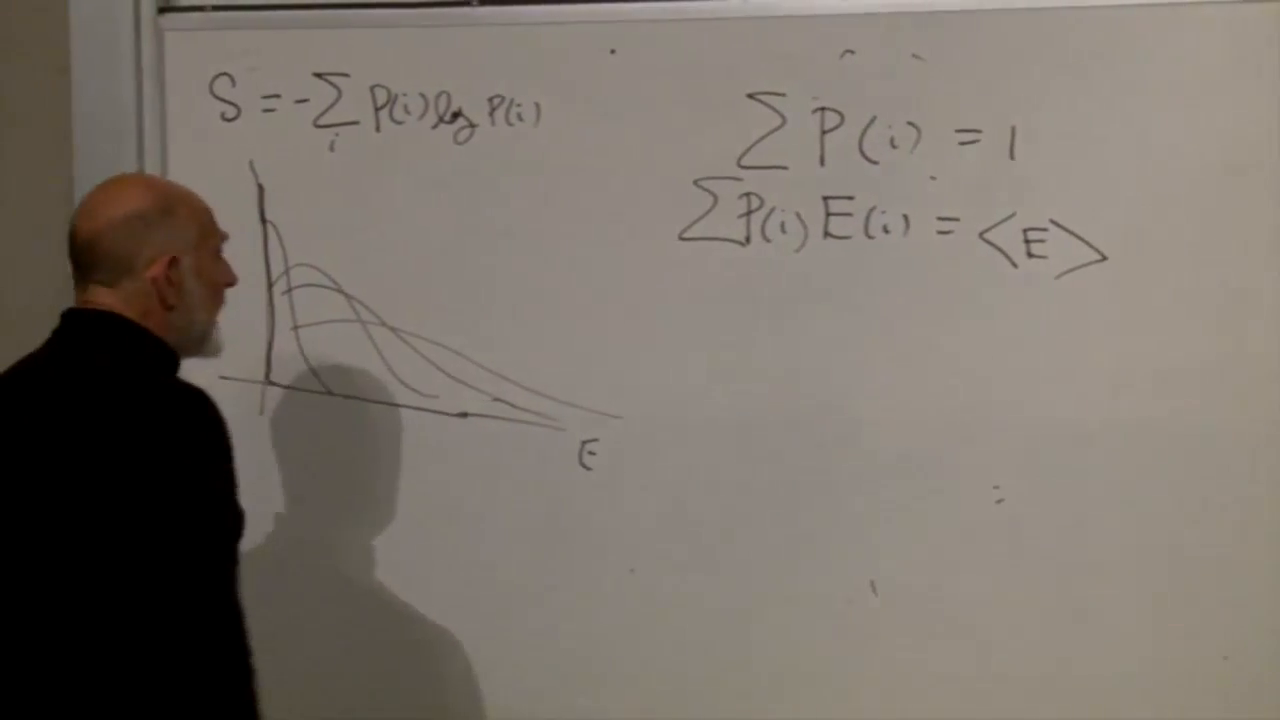
\includegraphics[width=0.88\textwidth]{lecture_03_figure_02.png}
\caption{Bảng mở đầu tập hợp các công thức entropy, chuẩn hóa và năng lượng
trung bình, cùng với một họ định tính các phân bố cân bằng.}
\lectureframe{00:06:44}
\end{figure}

\section{Cân bằng như một họ phân bố}

Bài giảng trước để lại cho ta một họ một tham số các phân bố cân bằng. Có
thể gán nhãn cho họ ấy bằng nhiệt độ, nhưng hiện giờ gán nhãn bằng năng lượng
trung bình \(\overline E\) hữu ích hơn. Ở mức năng lượng nhỏ nhất có thể, phân bố
tập trung vào một trạng thái cơ bản:
\[
 P_i=\delta_{i0}.
\]
Khi đó không còn bất định nào về trạng thái, và \(S=0\). Khi phân bố
cân bằng trải ra trên nhiều mức năng lượng hơn, cả năng lượng trung bình lẫn
entropy của nó đều tăng.

Đây là phát biểu về họ phân bố nhiệt, chứ không phải về mọi phân bố có thể
nghĩ ra. Một họ tùy ý có thể dịch về phía năng lượng lớn hơn đồng thời trở
nên hẹp hơn. Các phân bố cân bằng mà ta sắp suy ra không hành xử như vậy
trong miền nhiệt độ dương thông thường. Dọc theo họ đó,
\begin{equation}
 \frac{dS}{d\overline E}>0.
 \label{eq:sm3-positive-temperature-branch}
\end{equation}
Các hệ có phổ bị chặn cũng có thể có những nhánh mà trên đó đạo hàm này âm.
Những miền nhiệt độ âm đó là có thật, nhưng chúng được tạm gác sang một bên
trong lập luận này.

Cân bằng nhiệt có ý nghĩa nhiều hơn là sự đứng yên ở mức vi mô. Các phân tử
vẫn tiếp tục chuyển động, va chạm và trao đổi năng lượng. Điều trở nên dừng
theo thời gian là mô tả vĩ mô: phân bố không còn biểu lộ một độ trôi ròng,
và các phần tách biệt của hệ không còn duy trì một dòng năng lượng ròng.

\section{Các định luật nhiệt động lực học bằng ngôn ngữ thống kê}

Định luật thứ nhất là sự bảo toàn năng lượng. Định luật thứ hai phát biểu
rằng entropy nhiệt động lực học của một hệ vĩ mô cô lập không giảm:
\begin{equation}
 \Delta S_{\mathrm{tot}}\geq0.
 \label{eq:sm3-second-law}
\end{equation}
Dấu bằng mô tả trạng thái cân bằng hoặc một biến đổi thuận nghịch lý tưởng;
một quá trình thư giãn tự phát thông thường cho một sự tăng nghiêm ngặt.

Trong bức tranh xác suất, quá trình thư giãn có xu hướng phân tán trọng số
xác suất trên các khả năng vĩ mô mà ta vẫn còn phân biệt được. Phát biểu này
cần kèm theo sự lưu ý được nhấn mạnh trong bài giảng: ta đang \emph{làm thô}.
Sự tiến hóa Hamilton chính xác bảo toàn entropy hạt mịn của không gian pha.
Entropy vĩ mô tăng vì ta không còn theo dõi các tương quan và chi tiết vi mô.
Việc mất đi thông tin như vậy làm mô tả rút gọn rộng ra. Trái lại, một sự thu
hẹp tự phát sẽ có nghĩa là ta đã thu được thông tin vi mô mà không thực hiện
phép đo.

Định luật thứ không khẳng định rằng các hệ có thể đạt cân bằng nhiệt và rằng
trạng thái cân bằng có tính bắc cầu. Nếu \(A\) cân bằng với \(B\), và \(B\)
cân bằng với \(C\), thì \(A\) cân bằng với \(C\). Nhiệt độ cung cấp đại
lượng số làm cho tính bắc cầu này trở nên hiển nhiên:
\[
 T_A=T_B,\qquad T_B=T_C
 \quad\Longrightarrow\quad
 T_A=T_C.
\]
Khi chưa cân bằng, năng lượng truyền từ phân hệ có nhiệt độ lớn hơn sang
phân hệ có nhiệt độ nhỏ hơn. Khi nhiệt độ bằng nhau, dòng ròng chấm dứt. Bây
giờ ta suy ra phát biểu thao tác đó từ định nghĩa entropy của nhiệt độ.

\section{Vì sao năng lượng truyền từ nơi nóng sang nơi lạnh}

Xét hai phân hệ ghép yếu \(A\) và \(B\). Mỗi phân hệ đều đang cân
bằng nội bộ, nhưng nhiệt độ của chúng khác nhau. Chọn ký hiệu sao cho
\begin{equation}
 T_B>T_A>0.
 \label{eq:sm3-temperature-order}
\end{equation}
Trong một trao đổi nhỏ, bảo toàn năng lượng của hệ gộp cho
\begin{equation}
 dE_A+dE_B=0.
 \label{eq:sm3-energy-conservation}
\end{equation}
Định luật thứ hai cho
\begin{equation}
 dS_A+dS_B\geq0.
 \label{eq:sm3-entropy-change}
\end{equation}
Đối với mỗi phân hệ đang cân bằng nội bộ, nhiệt độ được định nghĩa bởi
\begin{equation}
 dE_X=T_X\,dS_X,
 \qquad X=A,B.
 \label{eq:sm3-temperature-differential}
\end{equation}
Thế vào \eqref{eq:sm3-energy-conservation}, ta được
\begin{equation}
 T_A\,dS_A+T_B\,dS_B=0,
\end{equation}
và do đó
\begin{equation}
 dS_B=-\frac{T_A}{T_B}\,dS_A.
 \label{eq:sm3-dsb}
\end{equation}
Đưa kết quả này vào \eqref{eq:sm3-entropy-change},
\begin{align}
 dS_{\mathrm{tot}}
 &=dS_A-\frac{T_A}{T_B}dS_A\\
 &=\frac{T_B-T_A}{T_B}\,dS_A\geq0.
 \label{eq:sm3-flow-entropy}
\end{align}
Vì \(T_B-T_A>0\) và \(T_B>0\), một trao đổi tự phát đòi hỏi
\[
 dS_A>0.
\]
Khi đó \eqref{eq:sm3-temperature-differential} cho
\begin{equation}
 dE_A=T_A\,dS_A>0,
 \qquad
 dE_B=-dE_A<0.
 \label{eq:sm3-hot-to-cold}
\end{equation}
Năng lượng đã truyền từ \(B\), phân hệ nóng hơn, sang \(A\), phân hệ
lạnh hơn. Ở đây, nhiệt đơn giản chỉ là năng lượng đang truyền. Dòng truyền
này tiếp tục cho đến khi \(T_A=T_B\), khi đó biến thiên entropy bậc nhất không
còn ưu tiên chiều nào nữa.

Cùng kết quả đó có thể được trình bày trong một dòng:
\begin{equation}
 dS_{\mathrm{tot}}
 =dE_A\left(\frac{1}{T_A}-\frac{1}{T_B}\right)\geq0.
 \label{eq:sm3-compact-flow}
\end{equation}
Dấu của hiệu nghịch đảo nhiệt độ quyết định dấu của \(dE_A\). Dạng gọn này
về sau sẽ phù hợp tự nhiên với tập hợp chính tắc.

\begin{classroomqa}
\audiencequestion{Lập luận này có giả thiết rằng \(A\) và \(B\) mỗi phân hệ đều đã
ở cân bằng nội bộ không?}
\lecturerresponse{Có. Việc gán một \(T_A\) hay \(T_B\) duy nhất đã bao hàm giả thiết
đó. Nếu một phân hệ chưa cân bằng nội bộ, hãy chia nó thành các vùng nhỏ hơn
và áp dụng lập luận này cục bộ ở bất cứ nơi nào có thể định nghĩa nhiệt độ.
Khi đó, quá trình thư giãn toàn cục được ghép lại từ các trao đổi giữa những
vùng ấy.
\lecturetimestamp{00:24:38--00:25:22}}
\end{classroomqa}

\section{Thế nào được coi là một trạng thái?}

Trước khi hỏi các xác suất cân bằng là gì, ta phải biết nhãn \(i\) có
nghĩa gì. Một trạng thái vi mô là mô tả đầy đủ nhất về hệ mà các định luật
vật lý cơ bản cho phép. Trong cơ học cổ điển, ta hình dung đó là các vị trí
và động lượng của mọi hạt. Trong cơ học lượng tử, thay vào đó, một trạng thái
là một trạng thái lượng tử đầy đủ; nguyên lý bất định ngăn cản việc xác định
sắc nét đồng thời mọi vị trí và động lượng cổ điển.

Đối với một hệ lượng tử trong một hộp hữu hạn, phép đếm trạng thái thích
hợp có thể là rời rạc. Cơ học thống kê cổ điển xuất hiện trong một giới hạn
thích hợp, nơi các tổng trên các trạng thái lượng tử sít nhau trở thành các
tích phân không gian pha. Quá trình lấy giới hạn đó cũng đưa vào ô không gian
pha cần thiết để làm cho entropy liên tục trở thành vô thứ nguyên; nó không
thu được chỉ bằng cách thay một dấu tổng bằng một dấu tích phân.

\begin{classroomqa}
\audiencequestion{Đối với một chất khí, có nên hình dung một trạng thái là vị trí và
động lượng của mọi phân tử không?}
\lecturerresponse{Đó là bức tranh cổ điển đúng. Tổng quát hơn, một trạng thái có nghĩa
là toàn bộ những gì về nguyên tắc có thể biết về hệ, phù hợp với các định
luật vật lý. Cơ học lượng tử làm thay đổi dạng của mô tả cực đại đó và khiến
phép đếm trong thể tích hữu hạn trở nên rời rạc. Việc khôi phục tích phân cổ
điển từ tổng lượng tử là một lập luận giới hạn thực sự, không phải một phép
thay thế trong một dòng.
\lecturetimestamp{00:25:31--00:27:38}}
\end{classroomqa}

\section{Một bể nhiệt tạo từ các bản sao}

Câu hỏi khó giờ đây không thể tránh khỏi: sau khi cân bằng đã được thiết
lập, điều gì quyết định \(P_i\)?

Đặt phân hệ tiếp xúc với một bể nhiệt rất lớn. Năng lượng có thể truyền qua
lại, nhưng bể có quá nhiều bậc tự do đến mức việc truyền một lượng năng lượng
nhỏ hầu như không làm thay đổi nhiệt độ của nó. Một bể đặc biệt thuận tiện
được tạo bởi nhiều bản sao ghép yếu của chính phân hệ đó. Một bản sao là hệ
đang được nghiên cứu; các bản sao còn lại cấu thành môi trường của nó.

Cách xây dựng này thường phản ánh một hệ vĩ mô thực. Hãy chia một vật thể
lớn gần như đồng nhất thành nhiều ô tương tự nhau. Mỗi ô là một phân hệ, còn
các ô còn lại đóng vai trò bể nhiệt của nó. Ký hiệu tổng số bản sao là \(N\).
Minh họa trên lớp dùng chín bản sao và ba nhãn trạng thái tô màu, nhưng phép
đếm không phụ thuộc vào những con số cụ thể đó.

Gọi \(n_i\) là số bản sao ở trạng thái \(i\). Đây là các
\emph{số chiếm đóng}. Có thể có vô hạn mức năng lượng khả dĩ, nhưng với tổng năng lượng hữu hạn thì phần lớn các mức rất cao có độ chiếm đóng không đáng kể hoặc bằng không.

Ràng buộc thứ nhất đơn giản là số bản sao:
\begin{equation}
 \sum_i n_i=N.
 \label{eq:sm3-number-constraint}
\end{equation}
Ràng buộc thứ hai là tổng năng lượng:
\begin{equation}
 \sum_i n_iE_i=N\overline E.
 \label{eq:sm3-total-energy-constraint}
\end{equation}
Vế phải là đại lượng quảng tính. Nếu số bản sao được nhân đôi trong khi trạng thái thống kê của chúng được giữ cố định, thì tổng năng lượng tăng gấp đôi, còn năng lượng trung bình trên mỗi bản sao vẫn là \(\overline E\).

\begin{classroomqa}
\audiencequestion{Việc xây dựng bằng bản sao có nhất thiết cũng phải thỏa một ràng buộc năng lượng không?}
\lecturerresponse{Có. Các số chiếm đóng phải cộng lại thành \(N\), và tổng có trọng số theo năng lượng của chúng phải bằng tổng năng lượng cố định \(N\overline E\).
Đó chính xác là hai ràng buộc mà về sau sẽ giới hạn cực đại entropy.
\lecturetimestamp{00:37:12--00:39:54}}
\end{classroomqa}

Xác suất để một bản sao được chọn ngẫu nhiên ở trạng thái \(i\) chính là tần suất tương đối của nó:
\begin{equation}
 P_i=\frac{n_i}{N},
 \qquad
 n_i=NP_i.
 \label{eq:sm3-frequency-probability}
\end{equation}

\begin{figure}[t]
\centering
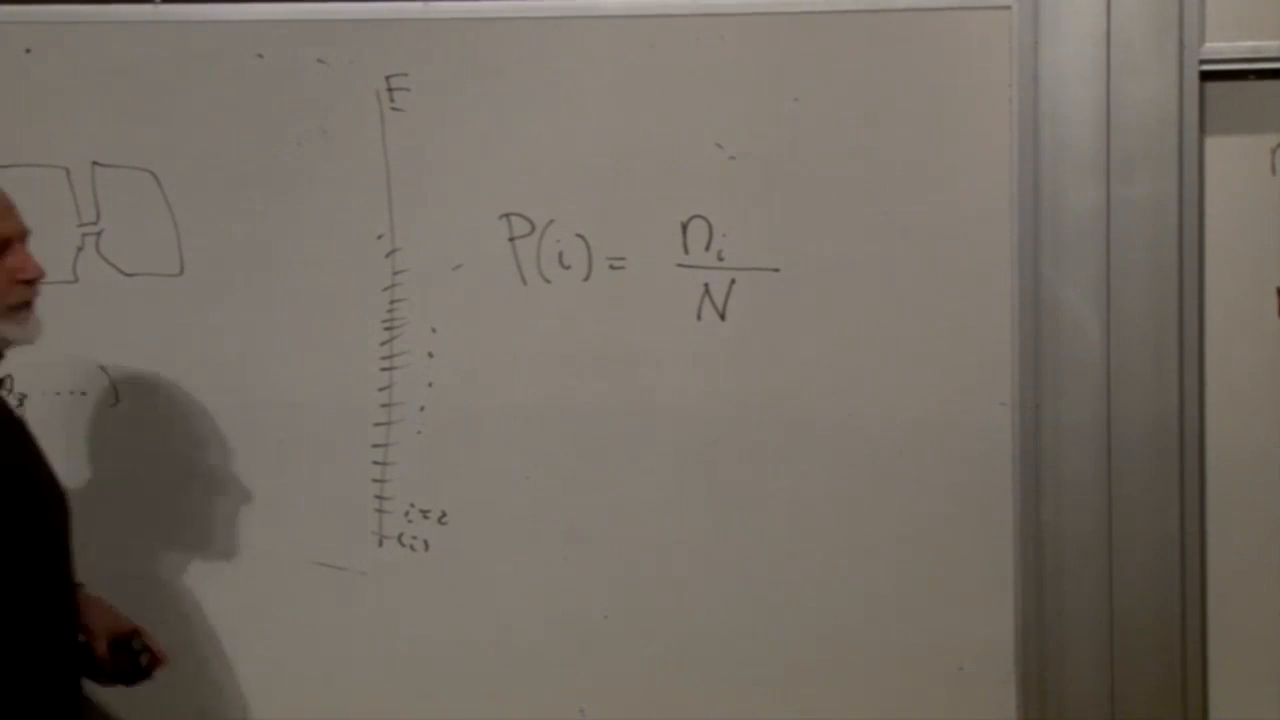
\includegraphics[width=0.82\textwidth]{lecture_03_figure_03.png}
\caption{Bức tranh mức năng lượng và việc đồng nhất xác suất với phần chiếm đóng \(P_i=n_i/N\).}
\lectureframe{00:41:40}
\end{figure}

\begin{classroomqa}
\audiencequestion{Ký hiệu \(N(i)\) trên bảng có được dùng với ý nghĩa khác \(n_i\) không?}
\lecturerresponse{Không. Cả hai đều ký hiệu số chiếm đóng của trạng thái \(i\). Ta dùng \(n_i\) một cách nhất quán và dành chữ hoa \(N\) cho tổng số bản sao.
\lecturetimestamp{00:41:28--00:41:33}}
\end{classroomqa}

Chia \eqref{eq:sm3-number-constraint} và
\eqref{eq:sm3-total-energy-constraint} cho \(N\) sẽ thu lại các ràng buộc xác suất:
\begin{equation}
 \sum_iP_i=1,
 \qquad
 \sum_iP_iE_i=\overline E.
 \label{eq:sm3-probability-constraints}
\end{equation}
Vì vậy, cách diễn giải xác suất theo tần suất trong ensemble đã tái tạo lại các phương trình mà ta đã bắt đầu.

\section{Độ bội của một mẫu chiếm đóng}

Cố định một tập số chiếm đóng \(\{n_i\}\). Có bao nhiêu cách phân các
\(N\) bản sao phân biệt được vào các trạng thái để thực hiện đúng tập ấy? Câu trả lời là hệ số đa thức
\begin{equation}
 C(\{n_i\})=\frac{N!}{\prod_i n_i!}.
 \label{eq:sm3-multiplicity}
\end{equation}
Để thấy được mẫu số, trước hết hãy sắp xếp tất cả \(N\) bản sao có nhãn theo \(N!\) thứ tự. Hoán vị các \(n_i\) bản sao chiếm cùng một trạng thái không tạo ra một cách phân bố chiếm đóng mới, nên phải chia cho \(n_i!\) đối với mỗi trạng thái.

\begin{figure}[t]
\centering
\includegraphics[width=0.88\textwidth]{lecture_03_figure_04.png}
\caption{Độ bội đa thức
\(C=N!/\prod_i n_i!\) được viết trên bảng.}
\lectureframe{00:46:55}
\end{figure}

Các mức không bị chiếm không gây vấn đề gì vì \(0!=1\). Nếu tất cả các bản sao đều chiếm một trạng thái, thì
\[
 C=\frac{N!}{N!}=1,
\]
đúng như dự kiến. Nếu ba bản sao chiếm ba trạng thái xác định khác nhau, thì
\[
 C=\frac{3!}{1!\,1!\,1!}=6.
\]
Với hai bản sao chiếm hai trạng thái xác định, công thức cho hai cách gán: hoán đổi bản sao có nhãn nào chiếm trạng thái nào.

\begin{classroomqa}
\audiencequestion{Có thể có hơn một tập số chiếm đóng thỏa hai ràng buộc không?}
\lecturerresponse{Thường thì có nhiều tập như vậy. Phương trình
\eqref{eq:sm3-multiplicity} trước hết đếm số cách sắp xếp cho một tập cố định
\(\{n_i\}\), mà chưa quyết định liệu nó có thỏa các ràng buộc hay không. Bước tiếp theo so sánh mọi tập tương thích với các ràng buộc và tìm tập nào có độ bội lớn nhất.
\lecturetimestamp{00:48:07--00:48:43}}
\end{classroomqa}

Giả thiết thống kê là các cách gán vi mô tương thích với cách bố trí cô lập được xử lý đối xứng. Vì thế, một mẫu chiếm đóng vĩ mô được thực hiện bởi nhiều cách gán hơn sẽ có xác suất lớn hơn. Với \(N\) lớn, phân bố theo các tỉ phần \(n_i/N\) trở nên nhọn rõ rệt. Các tỉ phần cân bằng là những giá trị làm cực đại \(C\), với các ràng buộc \eqref{eq:sm3-number-constraint} và
\eqref{eq:sm3-total-energy-constraint}.

\section{Xấp xỉ Stirling}

Các giai thừa trở nên khổng lồ từ rất lâu trước khi \(N\) đạt tới một giá trị vĩ mô, nên ta làm việc với logarit của chúng. Bắt đầu từ
\begin{equation}
 \log N!=\sum_{x=1}^{N}\log x.
 \label{eq:sm3-log-factorial-sum}
\end{equation}
Với \(N\) lớn, tổng được xấp xỉ bằng diện tích dưới \(\log x\):
\begin{align}
 \log N!
 &\simeq\int_1^N\log x\,dx\\
 &=\left[x\log x-x\right]_1^N\\
 &=N\log N-N+1.
 \label{eq:sm3-stirling-integral}
\end{align}
Nguyên hàm suy ra ngay từ
\[
 \frac{d}{dx}(x\log x-x)=\log x.
\]
Ở bậc quảng tính dẫn đầu, có thể bỏ hằng số cộng:
\begin{equation}
 \log N!\simeq N\log N-N.
 \label{eq:sm3-stirling-log}
\end{equation}
Lấy mũ cho ta dạng đơn giản được dùng trong bài giảng,
\begin{equation}
 N!\simeq N^N e^{-N}.
 \label{eq:sm3-stirling-simple}
\end{equation}

\begin{figure}[t]
\centering
\includegraphics[width=0.88\textwidth]{lecture_03_figure_05.png}
\caption{Xấp xỉ Stirling bậc dẫn đầu và phép suy ra nó bằng cách thay
tổng của \(\log x\) bằng một tích phân.}
\lectureframe{01:03:45}
\end{figure}

\begin{classroomqa}
\audiencequestion{Khi tính \(x\log x-x\) tại cận dưới, có xuất hiện thêm
\(+1\) không?}
\lecturerresponse{Có. Phương trình \eqref{eq:sm3-stirling-integral} có chứa
hằng số đó. Nó không đáng kể so với các số hạng tỉ lệ với \(N\) khi
\(N\to\infty\), đó là lý do công thức bậc dẫn đầu bỏ nó đi. Bản thân tổng
phải bắt đầu tại \(x=1\); \(\log0\) không xác định.
\lecturetimestamp{01:04:12--01:04:35}}
\end{classroomqa}

\begin{classroomqa}
\audiencequestion{Có phải cũng còn thiếu một thừa số tỉ lệ với \(\sqrt{N}\) không?}
\lecturerresponse{Có. Công thức tiệm cận sắc hơn là
\[
 N!\sim\sqrt{2\pi N}\left(\frac{N}{e}\right)^N.
\]
Logarit của nó chỉ thêm \(\tfrac12\log(2\pi N)\), là dưới quảng tính
so với \(N\log N-N\). Nó quan trọng đối với các xác suất chính xác khi \(N\)
 hữu hạn, nhưng không quan trọng đối với phép tính entropy bậc dẫn đầu của một hệ vĩ mô.
\lecturetimestamp{01:04:35--01:05:40}}
\end{classroomqa}

Xấp xỉ Stirling cũng phải được dùng cẩn trọng ở mẫu số của
\eqref{eq:sm3-multiplicity}. Trong giới hạn nhiệt động, các trạng thái mang
xác suất giới hạn khác không có \(n_i=NP_i\), nên số chiếm đóng của chúng tăng
cùng \(N\). Các trạng thái có độ chiếm đóng rất nhỏ hoặc triệt tiêu có thể được xử lý bằng một ngưỡng cắt năng lượng hữu hạn rồi khôi phục bằng một phép lấy giới hạn. Entropy quảng tính bậc dẫn đầu không bị ảnh hưởng bởi các số hạng dưới dẫn đầu đã lược bỏ.

\section{Logarit của độ bội là entropy}

Áp dụng \eqref{eq:sm3-stirling-simple} cho tử số và mọi thừa số ở mẫu có
chiếm đóng vĩ mô:
\begin{equation}
 C\simeq
 \frac{N^Ne^{-N}}
 {\prod_i n_i^{\,n_i}e^{-n_i}}.
 \label{eq:sm3-c-stirling}
\end{equation}
Vì \(\sum_i n_i=N\), các thừa số mũ bậc dẫn đầu triệt tiêu nhau:
\begin{equation}
 C\simeq\frac{N^N}{\prod_i n_i^{\,n_i}}.
 \label{eq:sm3-c-leading}
\end{equation}
Cực đại hóa logarit dễ hơn cực đại hóa một tích, và logarit là
đơn điệu, nên cả hai cực đại xuất hiện tại cùng một mẫu chiếm đóng:
\begin{equation}
 \log C=N\log N-\sum_i n_i\log n_i.
 \label{eq:sm3-logc-occupations}
\end{equation}
Bây giờ thay \(n_i=NP_i\):
\begin{align}
 \log C
 &=N\log N-\sum_iNP_i\log(NP_i)\\
 &=N\log N-N\sum_iP_i\log N
   -N\sum_iP_i\log P_i\\
 &=-N\sum_iP_i\log P_i,
 \label{eq:sm3-logc-entropy-derivation}
\end{align}
trong đó điều kiện chuẩn hóa làm triệt tiêu hai số hạng \(N\log N\). Do đó, ở bậc dẫn đầu theo \(N\),
\begin{equation}
 \boxed{\log C=NS}.
 \label{eq:sm3-logc-ns}
\end{equation}

\begin{figure}[t]
\centering
\includegraphics[width=0.88\textwidth]{lecture_03_figure_06.png}
\caption{Phép tính trên bảng nối
\(\log C=N\log N-\sum_i n_i\log n_i\) với
\(-N\sum_iP_i\log P_i=NS\).}
\lectureframe{01:16:10}
\end{figure}

Quan hệ này là trung tâm khái niệm của chương. Entropy không phải là một đại lượng không liên quan được áp đặt lên bài toán đếm. Nó là độ bội trên mỗi bản sao, được đo bằng logarit. Vì vậy, cực đại hóa số cách sắp xếp vi mô, ở bậc dẫn đầu, đồng nhất với cực đại hóa entropy của một bản sao.

\begin{classroomqa}
\audiencequestion{Không phải độ bội sẽ lớn nhất khi mọi số chiếm đóng đều bằng nhau sao?}
\lecturerresponse{Phân bố quả là đồng đều khi không trạng thái nào được phân biệt và chỉ có
\(\sum_i n_i=N\) được áp đặt trên một tập hữu hạn trạng thái. Ràng buộc năng lượng cố định
làm thay đổi câu trả lời vì các giá trị \(E_i\) là khác nhau.
Các số chiếm đóng bằng nhau nói chung không tạo ra năng lượng trung bình đã chỉ định.
\lecturetimestamp{01:17:07--01:18:20}}
\end{classroomqa}

\begin{classroomqa}
\audiencequestion{Chữ hoa \(N\) là lớn, nhưng vì sao có thể áp dụng xấp xỉ Stirling
cho mọi \(n_i\) ở mẫu?}
\lecturerresponse{Đối với mỗi trạng thái có xác suất giới hạn khác không,
\(n_i=NP_i\) tăng tỉ lệ với \(N\). Trước hết có thể giữ lại một miền
năng lượng hữu hạn, lấy giới hạn \(N\) lớn ở đó, rồi sau đó mở rộng miền ấy.
Các trạng thái ở đuôi thưa cần những hiệu chỉnh hữu hạn riêng, nhưng chúng không làm thay đổi
entropy quảng tính bậc dẫn đầu.
\lecturetimestamp{01:18:23--01:19:28}}
\end{classroomqa}

\begin{classroomqa}
\audiencequestion{Xấp xỉ \(N\) lớn này có phải là điều trước đó được hiểu là
làm thô không?}
\lecturerresponse{Không. Giới hạn nhiệt động chi phối các số chiếm đóng lớn
và phép đếm tiệm cận. Làm thô là sự mất đi hoặc sự loại bỏ có chủ ý
độ phân giải vi mô. Chúng là hai thao tác khác nhau, mặc dù cả hai thường được dùng trong cơ học thống kê vĩ mô.
\lecturetimestamp{01:19:29--01:19:46}}
\end{classroomqa}

\begin{classroomqa}
\audiencequestion{Vì
\(\log C=N\log N-\sum_i n_i\log n_i\), có phải số hạng thứ hai nên được cực tiểu hóa
thay vì cực đại hóa không?}
\lecturerresponse{Đúng; khi \(N\) cố định, cực đại hóa \(\log C\) tương đương
với cực tiểu hóa \(\sum_i n_i\log n_i\). Sau khi thay \(n_i=NP_i\), các
số hạng \(N\log N\) cố định triệt tiêu nhau và phần còn lại là
\(-N\sum_iP_i\log P_i=NS\). Vì thế, cùng một thao tác được mô tả tự nhiên
hơn là cực đại hóa entropy dương \(S\).
\lecturetimestamp{01:19:48--01:20:55}}
\end{classroomqa}

\begin{classroomqa}
\audiencequestion{Vì sao không kết thúc lập luận ngay bằng đối xứng và đặt
mọi \(n_i\) bằng nhau?}
\lecturerresponse{Lối tắt đó bỏ qua các nhãn năng lượng. Ràng buộc
chuẩn hóa đối xử các trạng thái một cách đối xứng, nhưng
\(\sum_iP_iE_i=\overline E\) thì không: các trạng thái có năng lượng khác nhau đóng góp
theo những cách khác nhau. Chính trong ràng buộc năng lượng mà phân bố cân bằng không đồng đều xuất hiện.
\lecturetimestamp{01:21:15--01:21:41}}
\end{classroomqa}

\section{Bài toán cực đại entropy}

Giờ đây ta có thể phát biểu quy tắc cơ học thống kê một cách không nhập nhằng. Hãy biến thiên các xác suất \(P_i\) và cực đại hóa
\begin{equation}
 S[P]=-\sum_iP_i\log P_i
 \label{eq:sm3-maximize-entropy}
\end{equation}
với các ràng buộc
\begin{equation}
 \sum_iP_i=1,
 \qquad
 \sum_iP_iE_i=\overline E.
 \label{eq:sm3-maxent-constraints}
\end{equation}
Các xác suất làm cực đại cho ta các tỉ phần chiếm đóng được ưu tiên rõ rệt của một tập hợp lớn các bản sao. Các số chiếm đóng có dao động, nhưng độ lệch tương đối của chúng co lại khi \(N\) tăng, nên các tỉ số \(n_i/N\) trở thành những xác suất nhiệt động lực học được xác định rõ.

\begin{classroomqa}
\audiencequestion{Có phải \(E_i\) là các năng lượng trạng thái cố định, còn ràng buộc thì dùng một tổng năng lượng được cho riêng hay không?}
\lecturerresponse{Đúng. Phổ \(\{E_i\}\) thuộc về hệ con.
Toàn bộ tập hợp các bản sao có một tổng năng lượng cố định, nhưng năng lượng
liên tục chuyển giữa các bản sao. Lấy tổng đó chia cho \(N\) sẽ cố định năng lượng
trung bình \(\overline E\) của một bản sao, chứ không phải năng lượng của nó trong từng hiện thực
vi mô.
\lecturetimestamp{01:26:12--01:27:07}}
\end{classroomqa}

Bài toán thì dễ phát biểu và vẫn chưa được giải. Đây là một bài toán cực trị với hai ràng buộc, nên cần thêm một công cụ toán học nữa.

\section{Các nhân tử Lagrange}

Đối với một hàm không bị ràng buộc \(F(x_1,x_2,\ldots)\), một điểm dừng
thỏa mãn
\begin{equation}
 \frac{\partial F}{\partial x_i}=0
 \qquad\text{for every }i.
 \label{eq:sm3-unconstrained-stationary}
\end{equation}
Bây giờ hãy thêm yêu cầu rằng
\begin{equation}
 G(x_1,x_2,\ldots)=0.
 \label{eq:sm3-one-constraint}
\end{equation}

\begin{classroomqa}
\audiencequestion{Nếu hình vẽ có các tọa độ \(x\)
và \(y\) thì \(x\) có nghĩa là gì?}
\lecturerresponse{Ở đây \(x\) là cách viết tắt cho toàn bộ véc-tơ tọa độ
\((x_1,x_2,\ldots)\). Trong hình vẽ hai chiều, các thành phần của nó
chỉ đơn giản là \(x\) và \(y\). Về sau các thành phần sẽ là các xác suất
\(P_1,P_2,\ldots\).
\lecturetimestamp{01:30:12--01:30:20}}
\end{classroomqa}

Về mặt hình học, các đường mức \(F=\text{constant}\) tạo thành một bản đồ đường đồng mức,
trong khi \(G=0\) là đường mà hệ được phép di chuyển trên đó. Một cực trị có ràng buộc xuất hiện ở nơi một
đường mức của \(F\) tiếp xúc với đường ràng buộc. Tại điểm đó, các gradient song song:
\begin{equation}
 \nabla F=-\lambda\nabla G
 \label{eq:sm3-parallel-gradients}
\end{equation}
với một số nào đó \(\lambda\).

\begin{figure}[t]
\centering
\includegraphics[width=0.88\textwidth]{lecture_03_figure_07.png}
\caption{Hình học đường đồng mức trên bảng và hàm bổ sung
\(F'=F+\lambda G\). Một cực trị có ràng buộc xuất hiện tại điểm tiếp xúc.}
\lectureframe{01:37:10}
\end{figure}

Có thể thu được phương trình \eqref{eq:sm3-parallel-gradients} bằng cách định nghĩa
hàm bổ sung
\begin{equation}
 F'=F+\lambda G
 \label{eq:sm3-augmented-function}
\end{equation}
và yêu cầu điều kiện dừng thông thường:
\begin{equation}
 \frac{\partial F'}{\partial x_i}=0.
 \label{eq:sm3-augmented-stationarity}
\end{equation}
Nhân tử \(\lambda\) ban đầu chưa biết. Điều đó không làm cho
hệ bị thiếu xác định, vì ràng buộc ban đầu \(G=0\) cung cấp thêm một
phương trình.

\begin{classroomqa}
\classquestion{Vì sao việc thêm một hạng tỉ lệ với \(G\) lại làm cho
điểm thỏa ràng buộc trở thành điểm dừng?}
\lecturerresponse{Tại cực trị có ràng buộc, một dịch chuyển tiếp tuyến với \(G=0\)
đã không tạo ra biến thiên bậc nhất nào của \(F\). Độ dốc duy nhất còn lại là
độ dốc theo pháp tuyến của ràng buộc. Vì \(\nabla G\) cũng hướng theo chính phương pháp tuyến
đó, nên một \(\lambda\) thích hợp sẽ triệt tiêu nó:
\(\nabla F+\lambda\nabla G=0\).
\lecturetimestamp{01:35:06--01:35:32}}
\end{classroomqa}

\section{Một ví dụ hai biến}

Tối thiểu hóa
\begin{equation}
 F(x,y)=\frac{x^2+y^2}{2}
 \label{eq:sm3-example-f}
\end{equation}
với ràng buộc
\begin{equation}
 x+y=1.
 \label{eq:sm3-example-constraint}
\end{equation}
Viết ràng buộc thành \(G=x+y-1=0\) và lập
\begin{equation}
 F'=\frac{x^2+y^2}{2}+\lambda(x+y-1).
 \label{eq:sm3-example-augmented}
\end{equation}
Các phương trình dừng là
\begin{align}
 \frac{\partial F'}{\partial x}&=x+\lambda=0,\\
 \frac{\partial F'}{\partial y}&=y+\lambda=0.
 \label{eq:sm3-example-derivatives}
\end{align}
Do đó \(x=y=-\lambda\). Phương trình còn lại là ràng buộc,
\[
 x+y=-2\lambda=1,
\]
nên
\begin{equation}
 \lambda=-\frac12,
 \qquad
 x=y=\frac12.
 \label{eq:sm3-example-solution}
\end{equation}
Điểm \((1/2,1/2)\) là nơi đường tròn nhỏ nhất có tâm tại gốc tọa độ
tiếp xúc với đường thẳng \(x+y=1\).

\begin{figure}[t]
\centering
\includegraphics[width=0.88\textwidth]{lecture_03_figure_08.png}
\caption{Phép tính hoàn chỉnh bằng phương pháp nhân tử Lagrange để tối thiểu hóa
\((x^2+y^2)/2\) với ràng buộc \(x+y=1\).}
\lectureframe{01:44:10}
\end{figure}

Với nhiều ràng buộc, hãy đưa vào một nhân tử cho mỗi ràng buộc:
\begin{equation}
 F'=F+\lambda_1G_1+\lambda_2G_2+\cdots.
 \label{eq:sm3-many-multipliers}
\end{equation}
Sau đó giải
\begin{equation}
 \begin{aligned}
 \frac{\partial F'}{\partial x_i}&=0
 &&\text{for every }i,\\
 G_a&=0
 &&\text{for every constraint }a.
 \end{aligned}
 \label{eq:sm3-many-equations}
\end{equation}
Bài giảng đề xuất một bài tập luyện được cố ý đặt ra một cách nhân tạo: tìm cực trị của một
hàm bậc hai của \(x,y,z\) đồng thời áp đặt hai ràng buộc tuyến tính độc lập,
chẳng hạn \(x+y=1\) và \(z+x=1\). Mục đích của nó không phải là đáp số cụ thể
mà là quy tắc rằng mỗi ràng buộc mang theo cả một nhân tử lẫn một
phương trình.

\section{Bài toán đã sẵn sàng cho bài giảng tiếp theo}

Đối với cơ học thống kê, các tọa độ là các xác suất
\(\{P_i\}\), hàm cần cực đại hóa là entropy, và các ràng buộc
là điều kiện chuẩn hóa và năng lượng trung bình cố định. Định nghĩa
\begin{align}
 S[P]&=-\sum_iP_i\log P_i,\\
 G_1[P]&=\sum_iP_i-1,\\
 G_2[P]&=\sum_iP_iE_i-\overline E.
 \label{eq:sm3-final-functions}
\end{align}
Vì vậy, hàm entropy bổ sung có thể được viết thành
\begin{equation}
 \Phi[P]
 =S[P]+\alpha G_1[P]+\beta G_2[P].
 \label{eq:sm3-final-augmented}
\end{equation}
Các phương trình cần giải là
\begin{equation}
 \frac{\partial\Phi}{\partial P_i}=0
 \quad\text{for every }i,
 \qquad
 G_1=0,
 \qquad
 G_2=0.
 \label{eq:sm3-final-problem}
\end{equation}

\begin{figure}[H]
\centering
\includegraphics[width=0.88\textwidth]{lecture_03_figure_09.png}
\caption{Bảng kết thúc: entropy như một hàm của các xác suất,
cùng với điều kiện chuẩn hóa và năng lượng trung bình cố định.}
\lectureframe{01:53:05}
\end{figure}

Đến đây bài toán đã được đặt ra đầy đủ. Giải
\eqref{eq:sm3-final-problem} sẽ cho ra phân bố cân bằng. Nhân tử
liên hợp với năng lượng sẽ trở thành nghịch đảo nhiệt độ
\(\beta=1/T\), tùy theo quy ước dấu được chọn trong
\eqref{eq:sm3-final-augmented}. Bài giảng tiếp theo sẽ thực hiện phép
lấy đạo hàm đó và thu được các trọng số Boltzmann.

\chapter{Trọng số Boltzmann, hàm phân hoạch và khí lý tưởng}

\lectureoverview{Chúng ta suy ra phân bố xác suất cân bằng bằng cách cực đại hóa entropy với điều kiện chuẩn hóa và năng lượng trung bình được giữ cố định. Hàm phân hoạch sau đó cho phép suy ra năng lượng trung bình, entropy và nhiệt độ bằng phép vi phân. Khí lý tưởng cung cấp ví dụ đầy đủ đầu tiên, tiếp theo là một mở rộng hấp dẫn và phần báo trước về dao động năng lượng.}

\section{Bài toán entropy có ràng buộc}

Bắt đầu với một tập hợp lớn gồm \(\mathcal N\) bản sao giống hệt nhau, tương tác với nhau rất yếu, của cùng một hệ con. Nếu \(n_i\) bản sao chiếm trạng thái thứ \(i\), thì
\begin{equation}
 p_i=\frac{n_i}{\mathcal N},
 \qquad
 \sum_i p_i=1.
 \label{eq:sm4-occupation-probability}
\end{equation}
Cách đếm đa thức của bài giảng trước cho entropy trên mỗi bản sao,
\begin{equation}
 S[p]=-\sum_i p_i\log p_i.
 \label{eq:sm4-entropy}
\end{equation}
Nên xem đây như một hàm thông thường của mọi biến \(p_1,p_2,\ldots\). Dạng cộng đơn giản của nó chính là điều làm cho phép tính này trở nên khả dĩ.

Tập hợp các bản sao có tổng năng lượng cố định là \(\mathcal N E\), trong đó
\(E\) là năng lượng trung bình trên mỗi bản sao. Vì vậy ràng buộc thứ hai là
\begin{equation}
 \sum_i p_iE_i=E.
 \label{eq:sm4-energy-constraint}
\end{equation}
Các mức \(E_i\) thuộc về hệ con; con số \(E\) ở vế phải là trung bình có trọng số theo xác suất của chúng. Việc cực đại hóa
\eqref{eq:sm4-entropy} với các ràng buộc
\eqref{eq:sm4-occupation-probability} và
\eqref{eq:sm4-energy-constraint} sẽ chọn ra các tỉ phần chiếm giữ có xác suất lớn áp đảo.

Để tiện lợi, hãy cực tiểu hóa \(-S=\sum_i p_i\log p_i\). Đưa vào một nhân tử Lagrange cho mỗi ràng buộc:
\begin{equation}
 \begin{aligned}
 \Phi[p;\alpha,\beta]
 &=\sum_i p_i\log p_i\\
 &\quad+\alpha\left(\sum_i p_i-1\right)\\
 &\quad+\beta\left(\sum_i p_iE_i-E\right).
 \end{aligned}
 \label{eq:sm4-augmented-functional}
\end{equation}
Các ký hiệu \(\alpha\) và \(\beta\) ở đây chưa hàm ý giả thiết vật lý nào. Ở giai đoạn này, chúng đơn giản chỉ là hai con số cần thiết để áp đặt hai ràng buộc.

\begin{classroomqa}
\audiencequestion{Phiếm hàm được bổ sung này cũng là một hàm của
\(\alpha\) và \(\beta\) phải không?}
\lecturerresponse{Đúng. Biến thiên nó theo \(\alpha\) và \(\beta\) sẽ thu lại hai ràng buộc. Tuy nhiên, trong phép tính trước mắt, ta giữ cố định các nhân tử đó và cho các xác suất \(p_i\) biến thiên. Các giá trị của chúng được cố định về sau bởi điều kiện chuẩn hóa và năng lượng trung bình đã cho.
\lecturetimestamp{00:09:32--00:09:49}}
\end{classroomqa}

\begin{figure}[t]
\centering
\includegraphics[width=0.92\textwidth]{lecture_04_figure_02.png}
\caption{Phiếm hàm entropy được bổ sung sau khi đã lược bỏ các hạng không đổi dưới phép biến thiên của các xác suất.}
\lectureframe{00:10:56}
\end{figure}

Khi lấy đạo hàm theo một xác suất, các hạng
\(-\alpha\) và \(-\beta E\) không đóng góp gì. Đây là phiếm hàm rút gọn xuất hiện trên bảng. Chúng vẫn là một phần của
\eqref{eq:sm4-augmented-functional}; chúng chỉ đơn thuần trở nên không còn liên quan đối với đạo hàm này.

\section{Phân bố Boltzmann}

Hãy chọn tùy ý một xác suất. Bài giảng chọn \(p_7\), phần vì
\(1\) trông quá đặc biệt và \(7\) là một con số may mắn. Không có gì phụ thuộc vào lựa chọn đó. Phép tính vi phân duy nhất cần dùng là
\begin{equation}
 \frac{d}{dp_i}\bigl(p_i\log p_i\bigr)=\log p_i+1.
\end{equation}
Do đó
\begin{equation}
 \frac{\partial\Phi}{\partial p_i}
 =\log p_i+1+\alpha+\beta E_i=0.
 \label{eq:sm4-stationarity}
\end{equation}
Giải theo \(p_i\),
\begin{align}
 \log p_i&=-(1+\alpha)-\beta E_i,\\
 p_i&=e^{-(1+\alpha)}e^{-\beta E_i}.
\end{align}
Thừa số thứ nhất không phụ thuộc vào nhãn trạng thái. Viết nó thành \(1/Z\):
\begin{equation}
 p_i=\frac{e^{-\beta E_i}}{Z}.
 \label{eq:sm4-boltzmann-weight}
\end{equation}

Đây là thành quả bất ngờ đầu tiên. Một phép đạo hàm có ràng buộc hoàn toàn thường quy đã tạo ra một định luật hàm mũ. Các xác suất tương đối tuân theo
\begin{equation}
 \frac{p_i}{p_j}=e^{-\beta(E_i-E_j)}.
 \label{eq:sm4-relative-weight}
\end{equation}
Nhân tử \(\beta\) kiểm soát tốc độ xác suất giảm theo năng lượng. Giá trị \(\beta\) dương lớn tập trung phân bố gần các mức thấp nhất; giá trị \(\beta\) dương nhỏ phân bố đáng kể trọng số lên các mức cao hơn của phổ. Ta đã có thể thấy rằng thay đổi \(\beta\) sẽ làm thay đổi năng lượng trung bình, mặc dù việc đồng nhất nó với nghịch đảo nhiệt độ vẫn còn phải được chứng minh.

\section{Chuẩn hóa và hàm phân hoạch}

Điều kiện chuẩn hóa xác định thừa số không phụ thuộc vào trạng thái:
\begin{equation}
 1=\sum_i p_i
 =\frac{1}{Z}\sum_i e^{-\beta E_i},
\end{equation}
cho nên
\begin{equation}
 Z(\beta)=\sum_i e^{-\beta E_i}.
 \label{eq:sm4-partition-function}
\end{equation}
Đây là hàm phân hoạch chính tắc. Ban đầu nó xuất hiện như một hằng số chuẩn hóa, nhưng cách mô tả đó đánh giá thấp nghiêm trọng vai trò của nó. Một khi \(Z(\beta)\) đã biết, các đại lượng nhiệt động học sẽ suy ra từ các đạo hàm của nó.

Các mức năng lượng trong \eqref{eq:sm4-partition-function} là dữ liệu đầu vào. Chúng
đến từ cơ học của hệ cùng với các điều kiện bên ngoài cố định: thể tích và hình dạng của hộp, các trường từ hoặc điện, và mọi tham số điều khiển khác. Thay đổi một tham số điều khiển sẽ làm thay đổi phổ và do đó làm thay đổi \(Z\). Trong phép tính hiện tại, các tham số ấy, và do đó tập \(\{E_i\}\), được giữ cố định.

\begin{classroomqa}
\audiencequestion{Chính xác thì các trục của bản phác thảo hàm mũ biểu diễn cái gì? Tọa độ thẳng đứng có phải là một \(p_i\) cụ thể không?}
\lecturerresponse{Độ cao được vẽ là xác suất gán cho một mức, còn thứ tự theo phương ngang có thể được hiểu hoặc là nhãn trạng thái
\(i\) hoặc, theo nghĩa vật lý hơn, là năng lượng \(E_i\). Mỗi trạng thái có một năng lượng cố định. Giá trị \(\beta\) lớn làm cho xác suất giảm rất dốc theo năng lượng đó; gần \(\beta=0\), các trọng số gần như phẳng trên các mức có thể tiếp cận.
\lecturetimestamp{00:19:39--00:20:09}}
\end{classroomqa}

\section{Năng lượng trung bình ẩn trong hàm phân hoạch}

Ràng buộc thứ hai xác định \(\beta\):
\begin{equation}
 E=\sum_i p_iE_i
 =\frac{1}{Z}\sum_i E_i e^{-\beta E_i}.
 \label{eq:sm4-mean-energy}
\end{equation}
Thay vì tính lại từ đầu tổng có trọng số này, hãy lấy đạo hàm của
\eqref{eq:sm4-partition-function}:
\begin{equation}
 \frac{dZ}{d\beta}
 =-\sum_i E_i e^{-\beta E_i}.
\end{equation}
So sánh với \eqref{eq:sm4-mean-energy} cho
\begin{equation}
 E(\beta)
 =-\frac{1}{Z}\frac{dZ}{d\beta}
 =-\frac{d\log Z}{d\beta}.
 \label{eq:sm4-energy-logz}
\end{equation}
Việc dùng logarit là tự nhiên vì đạo hàm của nó cung cấp thừa số
\(1/Z\).

\begin{figure}[t]
\centering
\includegraphics[width=0.82\textwidth]{lecture_04_figure_03.png}
\caption{Điều kiện chuẩn hóa, ràng buộc năng lượng trung bình và đạo hàm của hàm phân hoạch xuất hiện cùng nhau trên bảng.}
\lectureframe{00:26:24}
\end{figure}

\begin{classroomqa}
\audiencequestion{Phương trình ở phần dưới của bảng là một phương trình mới cho \(Z\), hay nó được suy ra từ định nghĩa ở phía trên?}
\lecturerresponse{Nó được suy ra bằng cách lấy đạo hàm của định nghĩa
\(Z=\sum_i e^{-\beta E_i}\). Phép đạo hàm đưa
\(-E_i\) xuống. Sau đó chia kết quả cho \(Z\) sẽ tái tạo lại tổng có trọng số dùng để định nghĩa năng lượng trung bình.
\lecturetimestamp{00:25:58--00:26:37}}
\end{classroomqa}

\begin{classroomqa}
\audiencequestion{Liệu
\(dZ/d\beta=-E Z\) có làm cho \(Z\) trở thành một hàm riêng của phép đạo hàm không?}
\lecturerresponse{Không theo nghĩa thông thường. Một phương trình trị riêng sẽ có một hằng số nhân với \(Z\), trong khi ở đây
\(E=E(\beta)\). Phương trình này cho ta năng lượng trung bình như một hàm của
\(\beta\); nó không phải là một bài toán trị riêng với trị riêng cố định.
\lecturetimestamp{00:28:49--00:29:43}}
\end{classroomqa}

Sự đơn giản của \eqref{eq:sm4-energy-logz} dễ gây ngộ nhận. Phổ có thể phức tạp, và việc tính \(Z\) có thể khó, nhưng một khi đã tìm được hàm duy nhất đó thì năng lượng trung bình suy ra chỉ bằng một đạo hàm. Mẫu hình này lặp lại xuyên suốt cơ học thống kê: các phép toán sơ cấp được áp dụng theo đúng thứ tự sẽ cho những kết quả mà khó có thể đoán trực tiếp.

\begin{classroomqa}
\audiencequestion{\(E\) là tổng năng lượng của tất cả các bản sao hay là năng lượng trung bình trên mỗi hộp?}
\lecturerresponse{Đó là năng lượng trung bình của một hộp. Tập hợp các bản sao có tổng năng lượng là \(\mathcal N E\). Về sau, khi chính hệ được chọn là cả một hộp chứa \(N\) hạt khí, thì \(E\) sẽ có nghĩa là năng lượng của toàn bộ mẫu khí đó.
\lecturetimestamp{00:30:55--00:31:10}}
\end{classroomqa}

\begin{classroomqa}
\audiencequestion{Ta có thể lấy logarit của
\(\sum_i e^{-\beta E_i}\) theo từng hạng được không?}
\lecturerresponse{Không. Logarit biến một tích thành một tổng, chứ không biến một tổng thành tổng các logarit:
\[
 \log\!\left(\sum_i e^{-\beta E_i}\right)
 \ne \sum_i\log\!\left(e^{-\beta E_i}\right).
\]
Sự phân biệt này về sau sẽ hữu ích, khi các hệ con độc lập khiến các hàm phân hoạch tương ứng nhân với nhau.
\lecturetimestamp{00:31:10--00:31:58}}
\end{classroomqa}

\section{Đại lượng nào được giữ cố định, và đại lượng nào được phép biến thiên?}

Trong cùng những công thức này có nhiều lớp biến số, và phần thảo luận trên lớp cố ý tách bạch chúng.

\begin{itemize}
 \item Các xác suất \(p_i\) là các ẩn ban đầu.
 \item Các mức \(E_i\) được giữ cố định một khi hệ và các tham số điều khiển của nó đã được chỉ định.
 \item Nhân tử \(\alpha\) đã được hấp thụ vào hệ số chuẩn hóa
 \(Z=e^{1+\alpha}\).
 \item Với một năng lượng trung bình \(E\) đã cho, ràng buộc sẽ cố định một số
 \(\beta\). Tuy nhiên, trên một họ các trạng thái cân bằng, có thể dùng
 \(E=E(\beta)\) hoặc \(\beta=\beta(E)\).
\end{itemize}

\begin{classroomqa}
\audiencequestion{Nếu các nhân tử là những con số, tại sao \(\beta\) và
\(E\) giờ lại được xem như các biến?}
\lecturerresponse{Đối với một bài toán có ràng buộc cụ thể, chúng quả thực là các con số.
Nhưng ta có thể so sánh nhiều bài toán cân bằng có cùng phổ và các năng lượng trung bình đã cho khác nhau. Trên họ đó, \(\beta\) thay đổi theo
\(E\). Giữ cố định \(E\) thì xác định \(\beta\); giữ cố định \(\beta\) thì xác định
\(E\). Đó là hai cách đọc của cùng một quan hệ.
\lecturetimestamp{00:31:58--00:33:27}}
\end{classroomqa}

\begin{classroomqa}
\audiencequestion{\(\alpha\) đã biến mất rồi sao?}
\lecturerresponse{Chỉ có tên gọi của nó là biến mất. Định nghĩa
\(e^{-(1+\alpha)}=1/Z\) hấp thụ nó vào \(Z\). Nếu giữ cả \(\alpha\)
và \(Z\) thì ta sẽ tính cùng một tham số chuẩn hóa hai lần.
\lecturetimestamp{00:33:29--00:33:49}}
\end{classroomqa}

Năng lượng không nhất thiết là đại lượng bảo toàn duy nhất. Nếu tổng động lượng, số hạt, mômen động lượng hoặc một đại lượng khác bị ràng buộc, thì giá trị kỳ vọng của nó sẽ có nhân tử riêng. Sự mở rộng đó làm thay đổi ensemble nhưng không thay đổi phương pháp.

\begin{classroomqa}
\audiencequestion{Liệu việc chỉ cố định năng lượng trung bình có giả định quá nhiều về hệ không?}
\lecturerresponse{Điều đó giả định rằng trong bài toán hiện tại không cần điều kiện hóa theo bất kỳ đại lượng bảo toàn nào khác. Nếu, chẳng hạn, tổng động lượng cũng được cố định, hãy thêm một ràng buộc nữa và một nhân tử Lagrange nữa. Trái lại, ở đây thể tích, hình dạng và các trường ngoài là những tham số điều khiển: chúng được giữ cố định và tự chúng xác định các mức năng lượng.
\lecturetimestamp{00:33:51--00:35:50}}
\end{classroomqa}

\begin{classroomqa}
\audiencequestion{Có nên cho \(\alpha\) xuất hiện như một đối số khác của năng lượng không, và \(Z\) có phụ thuộc vào các mức \(E_i\) không?}
\lecturerresponse{\(\alpha\) đã nằm trong \(Z\), nên nó không phải là một đối số độc lập. Hàm phân hoạch dĩ nhiên phụ thuộc vào phổ cố định cũng như vào \(\beta\). Việc thay đổi một tham số điều khiển sẽ làm thay đổi \(E_i\), và do đó làm thay đổi \(Z\); trong các đạo hàm theo \(\beta\) hiện tại thì phổ được giữ cố định.
\lecturetimestamp{00:35:52--00:37:10}}
\end{classroomqa}

\begin{classroomqa}
\audiencequestion{Chúng ta đang biến thiên các mức riêng lẻ \(E_i\), hay năng lượng trung bình \(E\)?}
\lecturerresponse{Các mức riêng lẻ được giữ cố định. Năng lượng trung bình thay đổi vì các xác suất thay đổi. Do đó, họ phân bố này được tham số hóa bởi \(E\) hoặc tương đương bởi \(\beta\), trong khi cùng một danh sách mức \(\{E_i\}\) được dùng xuyên suốt.
\lecturetimestamp{00:37:12--00:39:04}}
\end{classroomqa}

Trên thực tế, nhiệt độ thường dễ đo hơn nhiều so với tổng năng lượng của một chất khí. Ta có thể đặt một nhiệt kế vào; việc cân hiệu khối lượng tương đối tính và viện đến \(E=mc^2\) thì là đúng, nhưng cực kỳ không hữu ích. Để \(\beta\) mang ý nghĩa thao tác, giờ ta phải liên hệ nó với định nghĩa nhiệt động lực học của nhiệt độ.

\section{Entropy trước nhiệt độ}

Về mặt lôgic, entropy xuất hiện trước. Thế các xác suất Boltzmann vào
\eqref{eq:sm4-entropy}:
\begin{equation}
 \log p_i=-\beta E_i-\log Z.
\end{equation}
Khi đó
\begin{align}
 S
 &=-\sum_i p_i\log p_i\\
 &=\beta\sum_i p_iE_i+\log Z\sum_i p_i\\
 &=\beta E+\log Z.
 \label{eq:sm4-entropy-logz}
\end{align}
Tổng chuẩn hóa cung cấp thừa số 1 ở cuối. Đây cũng là gợi ý đầu tiên về năng lượng tự do Helmholtz, vì về sau
\(F_{\mathrm H}=-T\log Z\) trong các đơn vị với \(k_B=1\).

\begin{classroomqa}
\audiencequestion{Điều gì đã xảy ra với thừa số \(1/Z\) trong hạng thứ nhất?}
\lecturerresponse{Nó đã là một phần của \(p_i\). Tổng
\(\sum_i p_iE_i\) chứa xác suất đã chuẩn hóa đầy đủ và, theo định nghĩa, là năng lượng trung bình \(E\).
\lecturetimestamp{00:43:19--00:43:26}}
\end{classroomqa}

\begin{classroomqa}
\audiencequestion{Có nên có dấu trừ trong
\(S=\beta E+\log Z\) không?}
\lecturerresponse{Không. Entropy bắt đầu bằng một dấu trừ, còn
\(\log p_i=-\beta E_i-\log Z\) chứa thêm hai dấu trừ nữa. Chúng tạo ra hai hạng dương được hiển thị trong \eqref{eq:sm4-entropy-logz}.
\lecturetimestamp{00:45:53--00:46:03}}
\end{classroomqa}

Nhiệt độ được định nghĩa theo nhiệt động lực học bởi
\begin{equation}
 dE=T\,dS,
 \qquad
 \frac{1}{T}=\frac{dS}{dE},
 \label{eq:sm4-temperature-definition}
\end{equation}
trong khi mọi tham số điều khiển khác đều được giữ cố định. Một nỗ lực đầu tiên nhằm lấy đạo hàm \eqref{eq:sm4-entropy-logz} trực tiếp theo \(E\) nhanh chóng trở nên rối rắm vì \(\beta\) cũng phụ thuộc vào \(E\). Lấy vi phân toàn phần thì gọn hơn:
\begin{align}
 dS
 &=\beta\,dE+E\,d\beta
   +\frac{d\log Z}{d\beta}\,d\beta\\
 &=\beta\,dE+E\,d\beta-E\,d\beta\\
 &=\beta\,dE.
 \label{eq:sm4-entropy-differential}
\end{align}
Sự triệt tiêu dùng \eqref{eq:sm4-energy-logz}. So sánh
\eqref{eq:sm4-entropy-differential} với
\eqref{eq:sm4-temperature-definition} thu được
\begin{equation}
 T=\frac{1}{\beta},
 \qquad
 \beta=\frac{1}{T}.
 \label{eq:sm4-beta-temperature}
\end{equation}

\begin{figure}[t]
\centering
\includegraphics[width=0.82\textwidth]{lecture_04_figure_04.png}
\caption{Hai hạng \(d\beta\) triệt tiêu nhau, còn lại
\(dS=\beta\,dE\).}
\lectureframe{00:50:48}
\end{figure}

\begin{classroomqa}
\audiencequestion{Sự triệt tiêu này có giả định sai rằng
\(\log Z\) không phụ thuộc vào năng lượng hay nhiệt độ không?}
\lecturerresponse{Không. Với phổ cố định, chỉ có một tham số nhiệt độc lập. Ta có thể viết \(Z=Z(\beta)\), rồi xem
\(\beta=\beta(E)\) dọc theo họ cân bằng. Vi phân toàn phần giữ đầy đủ sự phụ thuộc theo \(d\beta\), và đồng nhất thức
\(d\log Z/d\beta=-E\) chính là điều làm cho sự triệt tiêu ấy hoạt động.
\lecturetimestamp{00:52:04--00:52:44}}
\end{classroomqa}

Trong phần lớn phép tính, nhiệt độ được đo theo đơn vị năng lượng, nên \(k_B=1\). Khôi phục các đơn vị phòng thí nghiệm,
\begin{equation}
 \beta=\frac{1}{k_B T_{\mathrm K}},
 \label{eq:sm4-beta-laboratory}
\end{equation}
trong đó \(T_{\mathrm K}\) là nhiệt độ tuyệt đối tính bằng kelvin. Thường tiện khi viết \(T_{\mathrm e}=k_BT_{\mathrm K}\) rồi dùng
\(\beta=1/T_{\mathrm e}\).

\begin{classroomqa}
\audiencequestion{Với một thể tích khí, hệ là một phân tử hay toàn bộ tập hợp?}
\lecturerresponse{Điều đó phụ thuộc vào cách ta định nghĩa hệ. Ở đây hệ sẽ là toàn bộ hộp khí, nên \(E\) là năng lượng của tất cả các phân tử của nó. Đối với một khí lý tưởng đủ loãng, một phân tử cũng có thể được xem là một phân hệ vì các hạt không tương tác; sự phân tích thành nhân tử dưới đây sẽ cho thấy mối liên hệ giữa hai cách mô tả.
\lecturetimestamp{00:53:32--00:54:49}}
\end{classroomqa}

Các hệ thức chính tắc giờ có thể được gom lại:
\begin{align}
 p_i&=\frac{e^{-\beta E_i}}{Z},&
 Z(\beta)&=\sum_i e^{-\beta E_i},\label{eq:sm4-canonical-pair}\\
 E&=-\frac{d\log Z}{d\beta},&
 S&=\beta E+\log Z,&
 T&=\frac{1}{\beta}.
 \label{eq:sm4-canonical-identities}
\end{align}

\section{Khí lý tưởng cổ điển}

Xét \(N\) hạt điểm đồng nhất khối lượng \(m\) trong một hộp có thể tích
\(V\). Chất khí là lý tưởng khi có thể bỏ qua các tương tác giữa các hạt. Đây có thể là một gần đúng tốt vì các lực yếu hoặc vì chất khí đủ loãng để các lần lại gần nhau ở cự li ngắn là hiếm.

Một vi trạng thái cổ điển được xác định bởi toàn bộ các vị trí và động lượng:
\begin{equation}
 (\bm q_1,\ldots,\bm q_N;\bm p_1,\ldots,\bm p_N).
\end{equation}
Có \(3N\) tọa độ vị trí và \(3N\) tọa độ động lượng, nên trạng thái là một điểm trong không gian pha \(6N\) chiều. Khi không có tương tác, Hamiltonian là
\begin{equation}
 H(\bm p)=\sum_{a=1}^{N}\frac{\bm p_a^2}{2m}
 =\sum_{\mu=1}^{3N}\frac{p_\mu^2}{2m}.
 \label{eq:sm4-ideal-hamiltonian}
\end{equation}

\begin{classroomqa}
\audiencequestion{Có phải có \(3N\) hạt không, và việc cộng trên mọi thành phần động lượng có đếm trùng các trạng thái không?}
\lecturerresponse{Có \(N\) hạt và \(3N\) thành phần động lượng. Tổng trong \eqref{eq:sm4-ideal-hamiltonian} chứa một hạng bậc hai cho mỗi thành phần. Khi đó, tích phân không gian pha tích phân trên mỗi thành phần độc lập đúng một lần, nên không có sự đếm trùng nào do tích đó gây ra.
\lecturetimestamp{01:02:29--01:04:04}}
\end{classroomqa}

Đối với một không gian pha cổ điển liên tục, tổng trên các trạng thái trở thành
\begin{equation}
 Z_N
 =\frac{1}{N!\,h^{3N}}
 \int_{V^N}d^{3N}q
 \int_{\mathbb R^{3N}}d^{3N}p\,
 e^{-\beta H(\bm p)}.
 \label{eq:sm4-classical-partition}
\end{equation}
Bài giảng tập trung vào các tích phân và viết cùng biểu thức ấy mà không có ô không gian pha \(h^{3N}\). Khôi phục nó khiến \(Z_N\) trở thành không thứ nguyên và phản ánh nguồn gốc lượng tử của việc đếm trạng thái cổ điển. Vì \(h\) độc lập với \(\beta\), nó không làm thay đổi đạo hàm dùng để tính năng lượng ở bên dưới.

Tích phân theo vị trí được tính ngay. Hamiltonian không phụ thuộc vào vị trí, và mỗi hạt có thể nằm ở bất kỳ đâu trong hộp:
\begin{equation}
 \int_{V^N}d^{3N}q=V^N.
\end{equation}
Tích phân theo động lượng phân tách thành \(3N\) tích phân Gauss một chiều giống hệt nhau:
\begin{equation}
 Z_N
 =\frac{V^N}{N!\,h^{3N}}
 \left[
  \int_{-\infty}^{\infty}dp\,
  e^{-\beta p^2/(2m)}
 \right]^{3N}.
 \label{eq:sm4-factorized-gas}
\end{equation}

Thừa số \(1/N!\) xem các cấu hình chỉ khác nhau bởi một hoán vị của các hạt đồng nhất là như nhau. Đối với năng lượng trung bình khi \(N\) và \(V\) được giữ cố định, nó chỉ đóng góp một hằng số độc lập với \(\beta\) vào \(\log Z_N\), nên biến mất dưới phép
\(-\partial/\partial\beta\). Nó không phải lúc nào cũng có thể bỏ đi: cùng với \(h^{3N}\), nó là thiết yếu để có một hàm phân hoạch không thứ nguyên, một entropy quảng tính và một thế hóa học nhất quán.

Giờ đặt
\begin{equation}
 x=\sqrt{\frac{\beta}{2m}}\,p,
 \qquad
 dp=\sqrt{\frac{2m}{\beta}}\,dx.
\end{equation}
Tích phân Gauss trở thành
\begin{align}
 \int_{-\infty}^{\infty}dp\,e^{-\beta p^2/(2m)}
 &=
 \sqrt{\frac{2m}{\beta}}
 \int_{-\infty}^{\infty}dx\,e^{-x^2}\\
 &=\sqrt{\frac{2\pi m}{\beta}}.
 \label{eq:sm4-gaussian}
\end{align}

\begin{figure}[t]
\centering
\includegraphics[width=0.82\textwidth]{lecture_04_figure_05.png}
\caption{Tích phân theo động lượng được đưa về Gaussian chuẩn chỉ bằng một phép đổi tỉ lệ.}
\lectureframe{01:13:12}
\end{figure}

Thế vào \eqref{eq:sm4-factorized-gas} thu được
\begin{equation}
 Z_N
 =\frac{V^N}{N!\,h^{3N}}
 \left(\frac{2\pi m}{\beta}\right)^{3N/2}.
 \label{eq:sm4-ideal-partition}
\end{equation}

\begin{figure}[t]
\centering
\includegraphics[width=0.78\textwidth]{lecture_04_figure_06.png}
\caption{Hàm phân hoạch của khí lý tưởng ở dạng hoàn chỉnh trên bảng. Ô không gian pha \(h^{3N}\) được khôi phục trong
\eqref{eq:sm4-ideal-partition}.}
\lectureframe{01:14:38}
\end{figure}

Sẽ hữu ích nếu viết cùng kết quả ấy theo bước sóng de Broglie nhiệt
\begin{equation}
 \lambda_T=\frac{h}{\sqrt{2\pi mT}}
 \qquad (k_B=1).
\end{equation}
Khi đó
\begin{equation}
 Z_N=\frac{1}{N!}\left(\frac{V}{\lambda_T^3}\right)^N.
 \label{eq:sm4-thermal-wavelength-form}
\end{equation}

Đối với \(N\) vĩ mô, công thức Stirling cho
\begin{equation}
 N!\simeq N^Ne^{-N}\sqrt{2\pi N}.
\end{equation}
Chỉ giữ lại phần phụ thuộc mũ trội và định nghĩa
\(\rho=N/V\),
\begin{equation}
 \frac{V^N}{N!}
 \simeq
 \frac{1}{\sqrt{2\pi N}}
 \left(\frac{e}{\rho}\right)^N.
 \label{eq:sm4-density-rewrite}
\end{equation}
Đây là cách sắp xếp lại gọn gàng theo mật độ của bài giảng. Thừa số căn bậc hai chỉ là hạng dưới trội trong \(\log Z_N\), nhưng ở đây nó được viết ra thay vì bị lặng lẽ bỏ đi.

\begin{classroomqa}
\audiencequestion{Nếu \(1/N!\) độc lập với \(\beta\), thì nó hoàn toàn không tạo ra khác biệt nào sao?}
\lecturerresponse{Nó không tạo ra khác biệt nào đối với đạo hàm của năng lượng trung bình đang xét khi \(N\) và \(V\) được giữ cố định, vì nó cộng một hằng số độc lập với \(\beta\) vào \(\log Z_N\). Tuy vậy, nó có ý nghĩa đối với entropy tuyệt đối và đối với các biến thiên của số hạt. Không nên nhầm lẫn mệnh đề về đạo hàm có phạm vi hạn chế này với mệnh đề rộng hơn về việc đếm trạng thái.
\lecturetimestamp{01:27:01--01:27:51}}
\end{classroomqa}

\section{Năng lượng và nguyên lý phân bố đều năng lượng}

Tích thì bất tiện khi lấy đạo hàm; logarit biến chúng thành tổng. Từ \eqref{eq:sm4-ideal-partition},
\begin{equation}
 \log Z_N
 =-\frac{3N}{2}\log\beta+\text{\(\beta\)-independent terms}.
 \label{eq:sm4-log-ideal-partition}
\end{equation}
Do đó
\begin{equation}
 E
 =-\frac{\partial\log Z_N}{\partial\beta}
 =\frac{3N}{2\beta}
 =\frac{3N}{2}T.
 \label{eq:sm4-ideal-energy}
\end{equation}
Năng lượng trên mỗi hạt là
\begin{equation}
 \frac{E}{N}=\frac{3}{2}T
 \qquad (k_B=1),
\end{equation}
hoặc, trong các đơn vị phòng thí nghiệm,
\begin{equation}
 \frac{E}{N}=\frac{3}{2}k_BT_{\mathrm K}.
 \label{eq:sm4-ideal-energy-lab}
\end{equation}

\begin{figure}[t]
\centering
\includegraphics[width=0.84\textwidth]{lecture_04_figure_07.png}
\caption{Chỉ hạng \(-3N\log\beta/2\) đóng góp vào năng lượng của khí lý tưởng, cho \(E/N=3T/2\).}
\lectureframe{01:25:28}
\end{figure}

\begin{classroomqa}
\audiencequestion{Hằng số Boltzmann đi vào công thức năng lượng ở đâu?}
\lecturerresponse{Nhiệt độ \(T\) theo cách dùng của nhà lý thuyết là một năng lượng. Để dùng kelvin, hãy thay nó bằng \(k_BT_{\mathrm K}\), thu được
\(E/N=3k_BT_{\mathrm K}/2\). Giá trị nhỏ của \(k_B\) chuyển một nhiệt độ có vẻ ở thang vĩ mô thành thang năng lượng vi mô của một phân tử.
\lecturetimestamp{01:24:58--01:26:01}}
\end{classroomqa}

Số 3 đến từ ba phương của không gian. Hệ số một phần hai đến từ sự phụ thuộc căn bậc hai của mỗi tích phân Gauss vào \(1/\beta\). Mỗi tọa độ động lượng bậc hai độc lập đóng góp
\begin{equation}
 \frac{1}{2}T
\end{equation}
vào năng lượng trung bình. Trong \(d\) chiều không gian, cùng lập luận ấy cho \(E/N=dT/2\). Đây là lần đầu tiên nguyên lý phân bố đều năng lượng xuất hiện.

Phép tính entropy được giao ở cuối bài giảng suy ra từ
\(S=\beta E+\log Z_N\). Dùng xấp xỉ Stirling,
\begin{equation}
 \frac{S}{N}
 \simeq
 \log\!\left[
  \frac{V}{N}
  \left(\frac{2\pi mT}{h^2}\right)^{3/2}
 \right]
 +\frac{5}{2},
 \label{eq:sm4-sackur-tetrode}
\end{equation}
đúng tới hiệu chỉnh dưới trội do \(N\) hữu hạn. Khôi phục \(k_B\) sẽ nhân vế phải với \(k_B\) và thay \(T\) bằng
\(k_BT_{\mathrm K}\). Kết quả này cho thấy rõ vì sao các hệ số chuẩn hóa đã triệt tiêu khỏi năng lượng lại là không thể thiếu đối với entropy.

\section{Đặt chất khí trong trường hấp dẫn}

Một câu hỏi về việc đặt chiếc hộp lên một sao neutron dẫn đến phần mở rộng có hấp dẫn. Trước khi xét một sao neutron, hãy xét một trường đều \(g\) trong một căn phòng bình thường. Chọn \(y=0\) ở đáy của một chiếc hộp có diện tích đáy \(A\) và chiều cao \(L\). Hamilton trở thành
\begin{equation}
 H=\sum_{a=1}^{N}
 \left(\frac{\bm p_a^2}{2m}+mgy_a\right).
 \label{eq:sm4-gravity-hamiltonian}
\end{equation}
Các tích phân theo vị trí ngang vẫn cho \(A^N\), còn mỗi tọa độ thẳng đứng đóng góp
\begin{equation}
 I_y(L)
 =\int_0^Ldy\,e^{-\beta mgy}
 =\frac{1-e^{-\beta mgL}}{\beta mg}.
 \label{eq:sm4-finite-height-integral}
\end{equation}

\begin{classroomqa}
\audiencequestion{Tích phân theo phương thẳng đứng thật sự nên lấy tới vô cực, hay chỉ tới đỉnh của hộp?}
\lecturerresponse{Đối với một hộp hữu hạn, nó phải chạy từ \(0\) đến chiều cao \(L\) của nó, như trong \eqref{eq:sm4-finite-height-integral}. Việc lấy cận trên ra vô cực là một phép đơn giản hóa về sau, mô hình hóa một khí quyển phía trên một bề mặt chứ không phải một căn phòng hữu hạn.
\lecturetimestamp{01:30:25--01:31:32}}
\end{classroomqa}

Vì thế, hàm phân hoạch đầy đủ cho trường hợp chiều cao hữu hạn là
\begin{equation}
 Z_N(L)
 =
 \frac{1}{N!\,h^{3N}}
 \left[
  A\,
  \frac{1-e^{-\beta mgL}}{\beta mg}
  \left(\frac{2\pi m}{\beta}\right)^{3/2}
 \right]^N.
 \label{eq:sm4-gravity-partition-finite}
\end{equation}
Thừa số theo phương thẳng đứng phụ thuộc vào \(\beta\), nên nó phải đóng góp vào năng lượng. Thật vậy,
\begin{equation}
 \langle U\rangle
 =N\left[
  \frac{1}{\beta}
  -\frac{mgL}{e^{\beta mgL}-1}
 \right].
 \label{eq:sm4-finite-gravity-energy}
\end{equation}
Điều này hoàn tất phần tích phân nhỏ mà lúc đầu bài giảng đã để lại như một phép tính phiền toái.

Đối với một khí quyển cao vô hạn, \(L\to\infty\), và
\begin{equation}
 I_y(\infty)=\frac{1}{\beta mg}.
\end{equation}
Hàm phân hoạch trở thành
\begin{equation}
 Z_N^{(\infty)}
 =
 \frac{1}{N!\,h^{3N}}
 \left[
  \frac{A}{\beta mg}
  \left(\frac{2\pi m}{\beta}\right)^{3/2}
 \right]^N.
 \label{eq:sm4-gravity-partition-infinite}
\end{equation}
Logarit phụ thuộc \(\beta\) của nó là
\begin{equation}
 \log Z_N^{(\infty)}
 =-\frac{3N}{2}\log\beta-N\log\beta+\mathrm{const}.
\end{equation}
Số hạng thứ nhất cho động năng \(3NT/2\); số hạng thứ hai cho thế năng hấp dẫn trung bình \(NT\). Do đó
\begin{equation}
 E_{\mathrm{tot}}=\frac{5N}{2}T
\end{equation}
đối với khí quyển không bị chặn được lý tưởng hóa này.

\begin{figure}[t]
\centering
\includegraphics[width=0.83\textwidth]{lecture_04_figure_08.png}
\caption{Hàm phân hoạch của khí quyển vô hạn bổ sung
\(-N\log\beta\) vào \(\log Z\), là nguồn gốc của thế năng trung bình.}
\lectureframe{01:36:38}
\end{figure}

\begin{classroomqa}
\audiencequestion{Một trường hấp dẫn rất mạnh có đòi hỏi thêm một nhân tử Lagrange khác không?}
\lecturerresponse{Không chỉ đơn thuần vì trường mạnh. Trọng lực làm thay đổi Hamilton và vì thế làm thay đổi các mức năng lượng hoặc trọng số trong không gian pha. Vẫn dùng cùng nhân tử năng lượng \(\beta\). Một sao neutron đưa vào những phức tạp vật lý bổ sung, nhưng sửa đổi đầu tiên vẫn là đưa thế năng hấp dẫn vào \(H\).
\lecturetimestamp{01:27:58--01:29:24}}
\end{classroomqa}

\section{Ba câu hỏi ở phần cuối}

\begin{classroomqa}
\audiencequestion{Phương trình nào là phân bố Boltzmann, và nó khẳng định điều gì về trạng thái cân bằng?}
\lecturerresponse{Phân bố là
\[
 p_i=\frac{e^{-\beta E_i}}{Z}.
\]
Đó là phân bố entropy cực đại dưới các ràng buộc chuẩn hóa và năng lượng trung bình cố định. Năng lượng trung bình phải được tính từ chính các xác suất ấy, và điều kiện chuẩn hóa vẫn phải được áp đặt dù trong công thức cuối cùng nó trông gần như tự động.
\lecturetimestamp{01:38:14--01:38:45}}
\end{classroomqa}

Quy trình này có thể tạo cảm giác máy móc: viết ra một hàm phân hoạch, lấy logarit, rồi lấy đạo hàm. Thế nhưng các phương trình thu được vẫn tiếp tục gây ngạc nhiên. Sự quen thuộc dạy ta phép toán đơn giản nào nên theo sau phép nào, nhưng nó không làm cho chủ đề này bớt kỳ thú.

\begin{classroomqa}
\audiencequestion{Có thể áp dụng những ý tưởng entropy này cho một ngôi sao đang sụp đổ hay một lỗ đen không? Làm sao entropy có thể tăng trong khi vật chất chiếm một vùng nhỏ hơn?}
\lecturerresponse{Các ngôi sao chủ yếu khó vì các chi tiết vật chất của chúng phức tạp. Lỗ đen có một chuẩn đối chiếu rõ ràng hơn: entropy Bekenstein--Hawking của nó là entropy hấp dẫn cực hạn đối với các ràng buộc vĩ mô đã cho. Sự sụp đổ có thể làm tăng entropy cho đến khi đạt tới giá trị của lỗ đen đó; để tăng thêm nữa thì cần thay đổi năng lượng sẵn có hoặc kích thước.
\lecturetimestamp{01:39:29--01:40:36}}
\end{classroomqa}

\begin{classroomqa}
\audiencequestion{Hàm phân hoạch cũng có thể tính các thăng giáng của năng lượng không?}
\lecturerresponse{Có. Một đạo hàm cho năng lượng trung bình, và đạo hàm bậc hai cho phương sai của nó:
\begin{align*}
 \frac{\partial^2\log Z}{\partial\beta^2}
 &=\langle E^2\rangle-\langle E\rangle^2\\
 &=\operatorname{Var}(E).
\end{align*}
Theo đơn vị năng lượng, đại lượng này liên hệ với nhiệt dung bởi
\(\operatorname{Var}(E)=T^2C_V\). Theo đơn vị phòng thí nghiệm,
\(\operatorname{Var}(E)=k_BT_{\mathrm K}^2C_V\). Hệ thức thăng giáng này là phép tính tiếp theo.
\lecturetimestamp{01:40:37--01:41:53}}
\end{classroomqa}

Các thăng giáng phân biệt cơ học thống kê với một mô tả nhiệt động lực học thuần túy liên tục. Việc nghiên cứu chúng một cách có hệ thống, đặc biệt gắn với Gibbs và Einstein, làm lộ ra các cấu phần vi mô hữu hạn đứng sau những định luật vĩ mô trơn tru. Đó là điểm bắt đầu của bài giảng tiếp theo.
\chapter{Áp suất, năng lượng tự do và thăng giáng năng lượng}

\lectureoverview{Ta suy ra áp suất từ hàm phân hoạch mà không giả định một bức tranh động học trong đó các phân tử va vào thành. Một bổ đề hình học chuyển một đạo hàm đoạn nhiệt thành các đạo hàm ở nhiệt độ cố định, năng lượng tự do Helmholtz làm cầu nối tới \(\log Z\), và định luật khí lý tưởng xuất hiện như ứng dụng đầu tiên. Sau đó ta dùng cùng hàm phân hoạch ấy để suy ra thăng giáng năng lượng cân bằng và quan hệ của nó với nhiệt dung.}

\section{Để toán học kiểm nghiệm trực giác}

Nhiệt động lực học có một danh tiếng khá đặc biệt. Phép tính của nó là sơ cấp, nhưng việc chọn lấy đạo hàm theo đại lượng nào và giữ cố định đại lượng nào có thể tinh tế đến mức đáng ngạc nhiên. Bài toán của ta được cố ý thu hẹp: tính áp suất của một khí lý tưởng. Tuy nhiên, con đường đi tới câu trả lời ấy được chủ ý làm đủ tổng quát cho những hệ trong đó bức tranh phân tử quen thuộc không còn đáng tin cậy nữa.

Câu chuyện động học thì dễ kể. Các phân tử va vào một bức tường và đảo dấu thành phần pháp tuyến của động lượng của chúng. Động lượng truyền trong một đơn vị thời gian cho ta lực, và lực trên một đơn vị diện tích cho ta áp suất. Ta đã biết rằng động năng trung bình trên mỗi phân tử trong ba chiều là
\begin{equation}
 \left\langle \frac{p^2}{2m}\right\rangle=\frac{3}{2}T
 \qquad (k_B=1).
 \label{eq:sm5-mean-kinetic-energy}
\end{equation}
Với một phân bố vận tốc đẳng hướng, ta có thể ước lượng tốc độ va chạm, độ truyền động lượng trong mỗi va chạm, và áp suất thu được.

Nhưng chính bức tường dường như lại phá vỡ tính đẳng hướng. Vì sao các phân tử rất gần biên lại phải có cùng phân bố về tốc độ và hướng như các phân tử ở sâu trong lòng hệ? Ở cân bằng thì đúng là như vậy, với độ chính xác thích hợp ở đây, nhưng kết luận ấy phải được suy ra từ cơ học thống kê chứ không nên bị lén đưa vào phép tính dưới dạng trực giác. Các va chạm giữa các phân tử còn khiến lập luận động học kém minh bạch hơn nữa. Khí không tương tác là dễ chính vì nó là một hệ đơn giản một cách khác thường.

Trong vật lý có những lúc thủ tục an toàn nhất là tạm thời gác bức tranh trực quan sang một bên và đi theo toán học. Ta xác định đại lượng cần tìm, thao tác các quan hệ tổng quát, rồi chờ cho tới khi xuất hiện một công thức dễ nhận ra. Trực giác quay trở lại ở cuối, nhưng khi đó toán học đang kiểm nghiệm trực giác chứ không phải ngược lại. Cái thú của nhiệt động lực học nằm ở những quan hệ bất ngờ nảy sinh từ thủ tục này.

Quan hệ ta cần là một phương trình trạng thái,
\begin{equation}
 P=P(T,V,N),
 \label{eq:sm5-equation-of-state-target}
\end{equation}
trong đó \(N\) là lượng vật chất, \(T\) là nhiệt độ và \(V\) là thể tích. Một phép suy dẫn thỏa đáng vẫn phải có nghĩa khi các hạt tương tác, hoặc khi vật chất là chất lỏng, plasma hay chất rắn. Chỉ việc đánh giá cuối cùng của hàm phân hoạch mới chuyên biệt cho khí lý tưởng.

\section{Entropy và năng lượng tự do Helmholtz}

Hãy bắt đầu bằng cách nhắc lại các công thức chính tắc sẽ cần đến về sau. Với các vi trạng thái được gắn nhãn bởi \(i\),
\begin{equation}
 \begin{aligned}
 S&=-\sum_i p_i\log p_i,\\
 p_i&=\frac{e^{-\beta E_i}}{Z},\\
 Z&=\sum_i e^{-\beta E_i}.
 \end{aligned}
 \label{eq:sm5-canonical-definitions}
\end{equation}
Logarit của xác suất là
\begin{equation}
 \log p_i=-\beta E_i-\log Z.
 \label{eq:sm5-log-probability}
\end{equation}
Thế vào entropy, ta được
\begin{align}
 S
 &=-\sum_i p_i\log p_i \notag\\
 &=\beta\sum_i p_iE_i+\log Z\sum_i p_i \notag\\
 &=\beta E+\log Z.
 \label{eq:sm5-entropy-log-z}
\end{align}
Ở đây \(E=\sum_i p_iE_i\) là năng lượng trung bình.

\begin{classroomqa}
\audiencequestion{Vì sao hạng thứ hai chỉ cho \(\log Z\), chứ không phải số trạng thái nhân với \(\log Z\)?}
\lecturerresponse{Hệ số đang được lấy tổng là \(p_i\), không phải \(1\).
Điều kiện chuẩn hóa cho \(\sum_i p_i=1\). Tương đương, tử số
\(\sum_i e^{-\beta E_i}=Z\) triệt tiêu \(Z\) ở mẫu. Số trạng thái không bao giờ xuất hiện ở bước này.
\lecturetimestamp{00:14:25--00:14:55}}
\end{classroomqa}

Trong các đơn vị năng lượng được dùng trong phần lớn bài giảng,
\(\beta=1/T\). Nhân \eqref{eq:sm5-entropy-log-z} với \(T\) rồi sắp xếp lại, ta được
\begin{equation}
 E-TS=-T\log Z.
 \label{eq:sm5-helmholtz-identity}
\end{equation}
Tổ hợp ở vế trái xuất hiện thường xuyên đến mức xứng đáng có một tên gọi:
\begin{equation}
 A\equiv E-TS,
 \qquad
 A=-T\log Z.
 \label{eq:sm5-helmholtz-definition}
\end{equation}
Đó là năng lượng tự do Helmholtz. Lúc này tên gọi kém quan trọng hơn chính đồng nhất thức ấy; ta sẽ cần đồng nhất thức đó khi áp suất được chuyển thành một đạo hàm của hàm phân hoạch.

\begin{figure}[t]
\centering
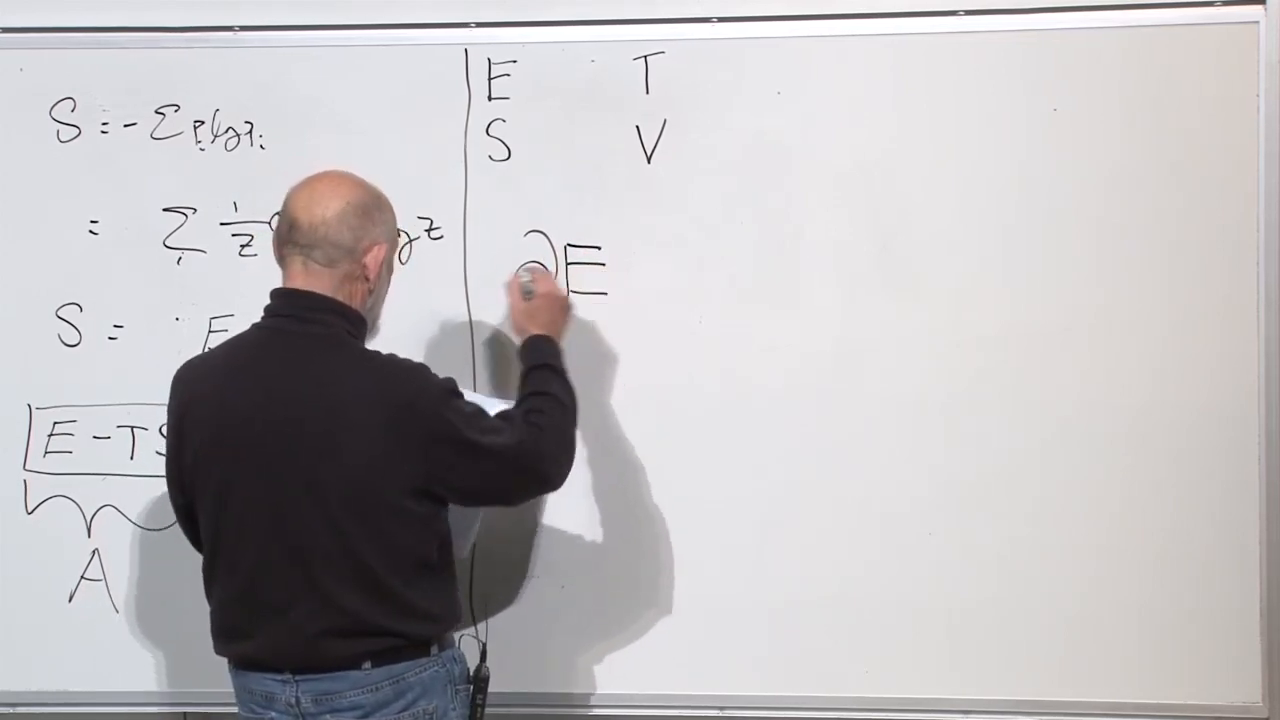
\includegraphics[width=0.90\textwidth]{lecture_05_figure_03.png}
\caption{Quan hệ entropy chính tắc được viết lại thành
\(A=E-TS=-T\log Z\).}
\lectureframe{00:16:50}
\end{figure}

\section{Các tham số điều khiển và các đáp ứng của chúng}

Một tham số điều khiển là một đại lượng vĩ mô mà nhà thực nghiệm có thể thay đổi từ bên ngoài. Di chuyển một pít-tông làm thay đổi thể tích mà không cần thao tác lên từng phân tử riêng lẻ. Điện trường và từ trường áp đặt từ bên ngoài là những ví dụ khác. Trong một quần thể thống kê tổng quát hơn, số hạt cũng có thể được phép thay đổi.

Các biến nhiệt động tự nhiên đi thành những cặp liên hợp. Trong bài toán hiện tại, thể tích là tham số điều khiển và áp suất là đáp ứng của nó. Ta thay đổi \(V\); áp suất cho ta biết hệ chống lại sự thay đổi ấy về mặt năng lượng như thế nào. Về sau, đạo hàm của năng lượng sẽ làm cho sự ghép cặp này trở nên chính xác.

\begin{classroomqa}
\audiencequestion{Bản thân áp suất có thể được xem là tham số điều khiển không?}
\lecturerresponse{Ta có thể thiết kế một thí nghiệm cố định áp suất ngoài, nhưng trong cách dựng dùng ở đây, vị trí pít-tông cố định thể tích và áp suất bên trong là đáp ứng. Áp suất và thể tích là các biến liên hợp; thành phần nào được điều khiển còn tùy vào quần thể và thiết bị.
\lecturetimestamp{00:19:22--00:20:01}}
\end{classroomqa}

\begin{classroomqa}
\audiencequestion{Có phải mọi phân tử đều được giả sử là đồng nhất, hay lập luận này chỉ giới hạn cho chất khí?}
\lecturerresponse{Không cần sự hạn chế nào như vậy cho lập luận nhiệt động. Xi lanh có thể chứa nhiều loại hạt, một chất lỏng, hoặc thậm chí một chất rắn đang bị nén. Hàm phân hoạch của khí lý tưởng sẽ chỉ là một áp dụng riêng sau khi công thức áp suất tổng quát đã được thiết lập.
\lecturetimestamp{00:20:02--00:20:39}}
\end{classroomqa}

\begin{classroomqa}
\audiencequestion{Lượng vật chất có thể được thay đổi như một thao tác ngoài khác không?}
\lecturerresponse{Có. Số hạt là một tham số điều khiển khả dĩ khác. Khi xét nó như một biến có thể thay đổi, ta đi tới đại lượng liên hợp riêng của nó, là thế hóa học. Trong phép tính tối nay, \(N\) được giữ cố định.
\lecturetimestamp{00:20:39--00:20:57}}
\end{classroomqa}

\begin{classroomqa}
\audiencequestion{Nước lỏng và hơi nước có thể hiện diện đồng thời trong cân bằng không?}
\lecturerresponse{Ở nhiệt độ và áp suất đồng tồn tại thì có thể. Trọng lực có thể đặt phần lỏng ở dưới phần hơi, nhưng hai pha vẫn có thể có cùng một nhiệt độ và duy trì cân bằng nhiệt. Cùng một khuôn khổ cơ học thống kê tổng quát vẫn áp dụng được.
\lecturetimestamp{00:20:59--00:21:36}}
\end{classroomqa}

Trong lập luận tiếp theo, hãy coi năng lượng và entropy là các hàm phụ thuộc của hai biến có thể điều chỉnh độc lập:
\begin{equation}
 E=E(T,V),
 \qquad
 S=S(T,V).
 \label{eq:sm5-dependent-functions}
\end{equation}
Nhiệt độ và thể tích cung cấp các tọa độ trên một không gian trạng thái nhiệt động. Năng lượng và entropy gán các giá trị số cho mọi điểm cân bằng trong không gian ấy.

\section{Đạo hàm ở entropy không đổi}

Đạo hàm cuối cùng ta cần đến là một đạo hàm khác thường:
\[
 \left(\frac{\partial E}{\partial V}\right)_S.
\]
Mặc dù \(T\) và \(V\) là các tọa độ độc lập, đạo hàm này yêu cầu ta thay đổi \(V\) đồng thời ràng buộc hàm phụ thuộc \(S(T,V)\) giữ không đổi. Đó là một đạo hàm dọc theo một đường cong trong mặt phẳng \((T,V)\), chứ không phải dọc theo một trục tọa độ.

\begin{classroomqa}
\audiencequestion{Làm sao \(T\) và \(V\) có thể độc lập nếu về sau lại dùng đạo hàm \(dT/dV\)?}
\lecturerresponse{Chúng độc lập trên toàn bộ không gian trạng thái. Một khi ta áp đặt ràng buộc \(S(T,V)=\mathrm{constant}\), các trạng thái được phép sẽ nằm trên một đường cong một chiều. Dọc theo đường đó, \(T\) trở thành một hàm của \(V\), và độ dốc của nó \(dT/dV\) được xác định rõ.
\lecturetimestamp{01:01:18--01:02:09}}
\end{classroomqa}

\begin{lemma}
Nếu \(E(T,V)\) và \(S(T,V)\) khả vi, thì ở mọi nơi mà
\((\partial S/\partial T)_V\neq0\),
\begin{equation}
 \left(\frac{\partial E}{\partial V}\right)_S
 =
 \left(\frac{\partial E}{\partial V}\right)_T
 -
 \left(\frac{\partial E}{\partial S}\right)_V
 \left(\frac{\partial S}{\partial V}\right)_T.
 \label{eq:sm5-calculus-lemma}
\end{equation}
\end{lemma}

\begin{proof}
Với một dịch chuyển vi phân bất kỳ,
\begin{equation}
 dE=
 \left(\frac{\partial E}{\partial V}\right)_T dV
 +
 \left(\frac{\partial E}{\partial T}\right)_V dT.
 \label{eq:sm5-total-differential-e}
\end{equation}
Khi giữ cố định \(V\), quy tắc dây chuyền cho phép dùng \(S\) làm biến trung gian:
\begin{equation}
 \left(\frac{\partial E}{\partial T}\right)_V
 =
 \left(\frac{\partial E}{\partial S}\right)_V
 \left(\frac{\partial S}{\partial T}\right)_V.
 \label{eq:sm5-chain-rule-e-s-t}
\end{equation}

Bây giờ hãy giới hạn dịch chuyển vào một đường cong mà trên đó \(S\) không đổi.
Dọc theo đường đó,
\begin{equation}
 0=dS=
 \left(\frac{\partial S}{\partial V}\right)_T dV
 +
 \left(\frac{\partial S}{\partial T}\right)_V dT.
 \label{eq:sm5-constant-entropy-differential}
\end{equation}
Giải theo độ dốc của đường cong, ta được
\begin{equation}
 \left(\frac{dT}{dV}\right)_S
 =
 -
 \frac{\left(\frac{\partial S}{\partial V}\right)_T}
 {\left(\frac{\partial S}{\partial T}\right)_V}.
 \label{eq:sm5-entropy-contour-slope}
\end{equation}
Chia \eqref{eq:sm5-total-differential-e} cho \(dV\), dùng
\eqref{eq:sm5-chain-rule-e-s-t}, rồi thế
\eqref{eq:sm5-entropy-contour-slope} vào:
\begin{align}
 \left(\frac{\partial E}{\partial V}\right)_S
 &=
 \left(\frac{\partial E}{\partial V}\right)_T
 +
 \left(\frac{\partial E}{\partial S}\right)_V
 \left(\frac{\partial S}{\partial T}\right)_V
 \left(\frac{dT}{dV}\right)_S \notag\\
 &=
 \left(\frac{\partial E}{\partial V}\right)_T
 -
 \left(\frac{\partial E}{\partial S}\right)_V
 \left(\frac{\partial S}{\partial V}\right)_T.
\end{align}
Thừa số \((\partial S/\partial T)_V\) đã triệt tiêu, qua đó chứng minh kết quả.
\end{proof}

\begin{figure}[t]
\centering
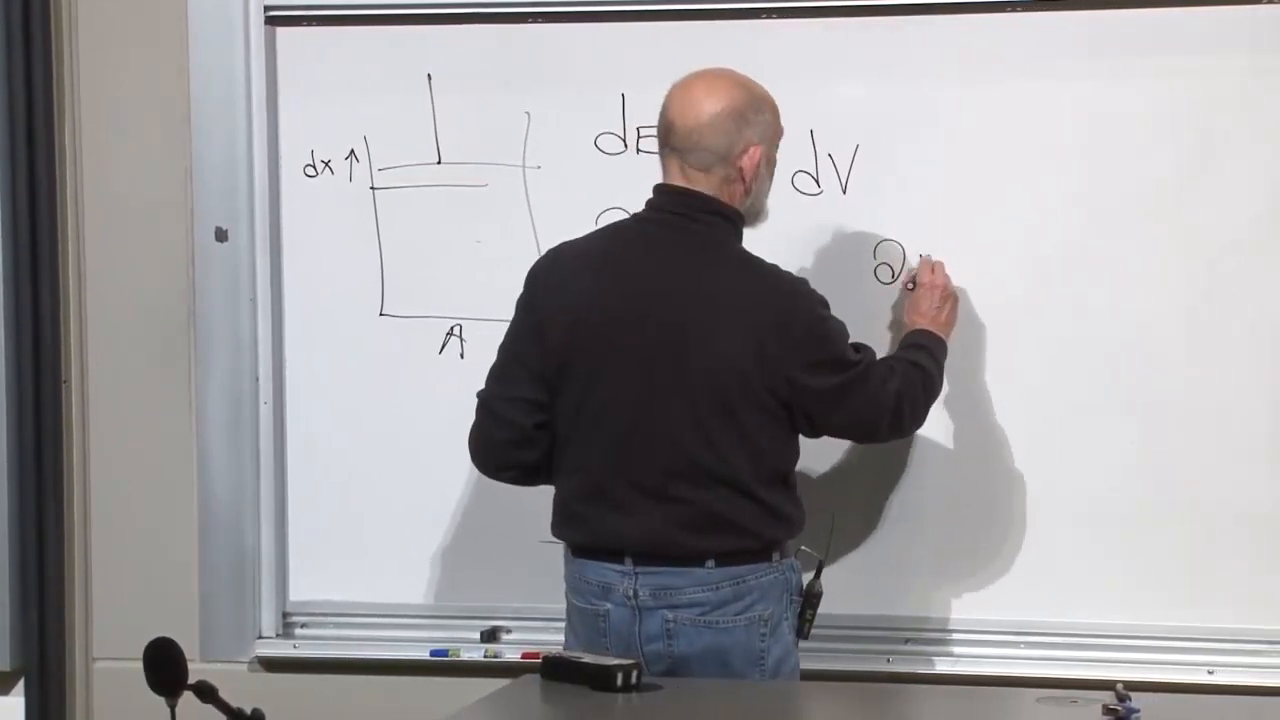
\includegraphics[width=0.90\textwidth]{lecture_05_figure_04.png}
\caption{Phép tính trên đường mức entropy không đổi tại bước triệt tiêu, bước hoàn tất bổ đề về đạo hàm.}
\lectureframe{00:36:10}
\end{figure}

Bức tranh hình học không phải chỉ để trang trí. Nó giải thích vì sao một đạo hàm có vẻ lạ ở \(S\) không đổi có thể được tính bằng các đạo hàm riêng thông thường theo các tọa độ độc lập \(T\) và \(V\). Việc viết \(\delta E/\delta V\) trong quá trình xây dựng là một lời nhắc hữu ích rằng các ký hiệu ấy biểu diễn những tỉ số của các biến thiên nhỏ dọc theo một đường đi đã được chỉ rõ.

\begin{classroomqa}
\audiencequestion{Khai triển của \(dE\) có phải chỉ là định nghĩa thông thường của các đạo hàm riêng không?}
\lecturerresponse{Có. Không có gì đặc biệt xảy ra trong vi phân toàn phần. Yếu tố thêm vào duy nhất là sự hạn chế về sau vào đường cong \(dS=0\), vốn xác định quan hệ giữa \(dT\) và \(dV\).
\lecturetimestamp{00:29:26--00:29:32}}
\end{classroomqa}

\begin{classroomqa}
\audiencequestion{Có phải để triệt tiêu được thì
\((\partial S/\partial T)_V\) phải khác không?}
\lecturerresponse{Có. Đối với một hệ ổn định thông thường,
\[
 \left(\frac{\partial S}{\partial T}\right)_V
 =\frac{C_V}{T}>0,
\]
nên phép chia là hợp lệ. Những điểm ngoại lệ đòi hỏi phải được xét riêng.
Khi Hamiltonian được giữ cố định, tăng nhiệt độ làm phân bố năng lượng chính tắc rộng ra và thông thường làm entropy tăng; hạ nhiệt độ làm nó hẹp lại. Đây là hướng đúng về mặt vật lý của lập luận về tính đơn điệu.
\lecturetimestamp{00:36:50--00:37:47}}
\end{classroomqa}

\section{Công của pít-tông và điều kiện đoạn nhiệt}

Bây giờ ta gán cho đạo hàm này một ý nghĩa vật lý. Hãy xét một pít-tông có
tiết diện ngang \(\mathcal A\). Nếu nó dịch ra ngoài một đoạn \(dx\), thì
\begin{equation}
 dV=\mathcal A\,dx.
 \label{eq:sm5-piston-volume}
\end{equation}
Khí tác dụng lực \(P\mathcal A\) lên pít-tông, nên công do khí thực hiện là
\begin{equation}
 \delta W_{\mathrm{by}}=P\mathcal A\,dx=P\,dV.
 \label{eq:sm5-piston-work}
\end{equation}
Nếu không có nhiệt đi vào khí, định luật bảo toàn năng lượng cho
\begin{equation}
 dE=-P\,dV.
 \label{eq:sm5-adiabatic-work}
\end{equation}
Dấu này có ý nghĩa vật lý: trong quá trình giãn nở, khí nâng pít-tông lên hoặc gia tốc cho nó, và năng lượng của chính khí giảm đi.

\begin{figure}[t]
\centering
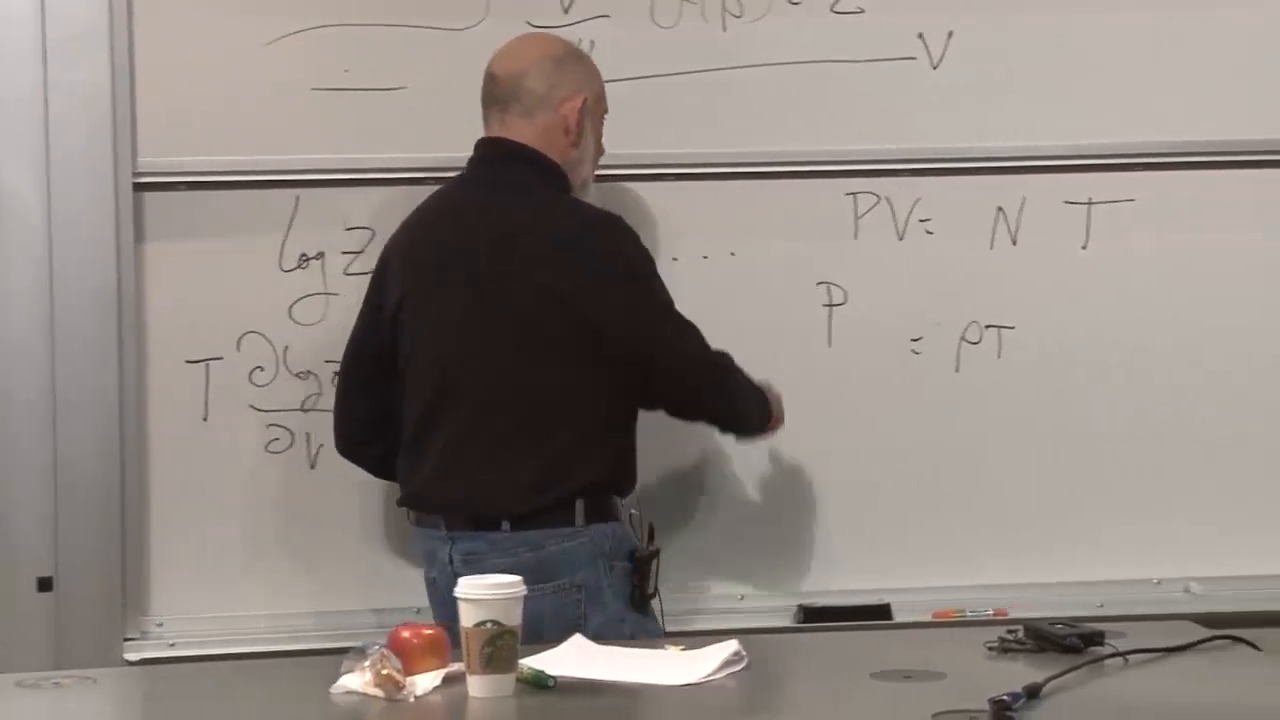
\includegraphics[width=0.90\textwidth]{lecture_05_figure_05.png}
\caption{Hình học của pít-tông và hệ thức công suy ra được
\(dE=-P\,dV\).}
\lectureframe{00:43:10}
\end{figure}

Hai lưu ý là thiết yếu. Pít-tông phải chuyển động đủ chậm để
hệ luôn ở gần cân bằng đến mức tùy ý, và thành bình phải được
cách nhiệt để năng lượng không được cung cấp dưới dạng nhiệt. Một sự kéo ra nhanh có thể
nhanh đến mức không phân tử nào chạm tới pít-tông đang lùi trong khi nó chuyển động. Một
sự nén nhanh tạo ra sóng xung kích. Không quá trình nào trong hai quá trình ấy được biểu diễn bằng
một dãy trạng thái cân bằng.

Từ \emph{đoạn nhiệt} đôi khi được dùng để chỉ không có truyền nhiệt và
đôi khi để chỉ biến đổi chậm. Trong quá trình thuận nghịch cần có ở đây, cả hai
ý đều tham gia: biến đổi là quasi-tĩnh và được cách nhiệt. Trong các điều
kiện đó, nó cũng là đẳng entropy.

\begin{classroomqa}
\audiencequestion{Vì sao một biến đổi đoạn nhiệt giữ entropy cố định?}
\lecturerresponse{Hãy nhìn hệ theo cơ học lượng tử. Các mức
năng lượng nhiều hạt của nó phụ thuộc vào thể tích. Khi \(V\) thay đổi chậm, định lý đoạn nhiệt
đưa mỗi mức đang bị chiếm liên tục sang mức tương ứng tiếp theo của nó mà không có
chuyển giữa các nhãn mức. Các năng lượng \(E_i(V)\) thay đổi, nhưng các
xác suất chiếm \(p_i\) vẫn giữ nguyên. Vì
\(S=-\sum_i p_i\log p_i\) phụ thuộc vào các xác suất đó, entropy vẫn
không đổi. Sự trao đổi nhiệt hoặc chuyển động không thuận nghịch sẽ làm kết luận
này không còn đúng.
\lecturetimestamp{00:43:37--00:49:15}}
\end{classroomqa}

\begin{figure}[t]
\centering
\includegraphics[width=0.90\textwidth]{lecture_05_figure_06.png}
\caption{Các mức năng lượng nhiều hạt biến thiên theo thể tích trong khi các
xác suất chiếm của chúng vẫn giữ nguyên các nhãn mức.}
\lectureframe{00:48:50}
\end{figure}

Phương trình \eqref{eq:sm5-adiabatic-work}, khi được đánh giá dọc theo đường
entropy không đổi này, xác định áp suất là
\begin{equation}
 P=-\left(\frac{\partial E}{\partial V}\right)_S.
 \label{eq:sm5-pressure-fixed-entropy}
\end{equation}
Đây là hệ thức liên hợp giữa áp suất và thể tích.

\begin{classroomqa}
\audiencequestion{Điều gì xảy ra nếu thay vào đó pít-tông được dịch chuyển nhanh?}
\lecturerresponse{Hệ rời khỏi cân bằng và động lực học chi tiết của nó
trở nên quan trọng. Nén đột ngột tạo ra một sóng xung kích. Trong một sự giãn nở tự do lý tưởng,
pít-tông có thể lùi đi trước khi bất kỳ phân tử nào va vào nó, nên không có công nào được thực hiện và
năng lượng vẫn giữ nguyên dù thể tích thay đổi. Về sau khí
thư giãn về cân bằng với entropy tăng lên. Những quá trình như vậy không thể được
mô tả bằng đạo hàm cân bằng duy nhất trong
\eqref{eq:sm5-pressure-fixed-entropy}.
\lecturetimestamp{00:58:30--01:01:15}}
\end{classroomqa}

\begin{classroomqa}
\audiencequestion{Điều kiện định lượng nào quyết định một biến đổi có
chậm hay không?}
\lecturerresponse{Thời gian biến thiên của tác động bên ngoài phải dài so với
các thời gian thư giãn nội tại liên quan. Đối với một chất khí, nhiều va chạm
phân tử và nhiều lần va vào thành phải xảy ra trong suốt biến đổi vĩ mô.
Thang thời gian chính xác phụ thuộc vào vật liệu và hình học, còn bản thân
giới hạn quasi-tĩnh thì là tổng quát.
\lecturetimestamp{01:02:09--01:03:20}}
\end{classroomqa}

\section{Từ năng lượng đoạn nhiệt đến hàm phân hoạch}

Công thức vật lý \eqref{eq:sm5-pressure-fixed-entropy} vẫn chưa phải là công thức
dễ tính. Cơ học thống kê chính tắc tự nhiên cung cấp
các hàm theo nhiệt độ, vì \(T\) xuất hiện trực tiếp trong
trọng số Boltzmann. Bổ đề giải tích chuyển đạo hàm ở entropy cố định, vốn bất tiện,
sang ngôn ngữ tính toán đó:
\begin{align}
 P
 &=
 -\left(\frac{\partial E}{\partial V}\right)_T
 +
 \left(\frac{\partial E}{\partial S}\right)_V
 \left(\frac{\partial S}{\partial V}\right)_T.
 \label{eq:sm5-pressure-lemma-substitution}
\end{align}
Ở thể tích cố định, định luật một cho \(dE=T\,dS\), và do đó
\begin{equation}
 \left(\frac{\partial E}{\partial S}\right)_V=T.
 \label{eq:sm5-e-s-temperature}
\end{equation}
Vì vậy
\begin{equation}
 P=
 -\left(\frac{\partial E}{\partial V}\right)_T
 +
 T\left(\frac{\partial S}{\partial V}\right)_T.
 \label{eq:sm5-pressure-fixed-temperature-pieces}
\end{equation}

\begin{classroomqa}
\audiencequestion{Dấu trừ trong công thức áp suất bắt nguồn từ
đâu?}
\lecturerresponse{Nó bắt nguồn từ công do khí thực hiện:
\(dE=-P\,dV\) trong giãn nở đoạn nhiệt. Bản thân bổ đề giải tích có một
dấu trừ giữa hai hạng của nó; dấu trừ toàn cục trong
\(P=-(\partial E/\partial V)_S\) đảo dấu của cả hai hạng ấy, cho ra
\eqref{eq:sm5-pressure-fixed-temperature-pieces}.
\lecturetimestamp{00:52:40--00:53:14}}
\end{classroomqa}

Bởi vì \(T\) được giữ cố định trong cả hai đạo hàm,
\begin{align}
 P
 &=
 -\left(\frac{\partial}{\partial V}(E-TS)\right)_T \notag\\
 &=
 -\left(\frac{\partial A}{\partial V}\right)_T.
 \label{eq:sm5-pressure-free-energy}
\end{align}
Cuối cùng thay \(A=-T\log Z\) vào:
\begin{equation}
 \boxed{
 P=
 T\left(\frac{\partial\log Z}{\partial V}\right)_T
 }.
 \label{eq:sm5-pressure-log-z}
\end{equation}

\begin{figure}[t]
\centering
\includegraphics[width=0.90\textwidth]{lecture_05_figure_07.png}
\caption{Phiên bản cô đọng ở nhiệt độ cố định của lập luận:
\(P=-(\partial A/\partial V)_T
=T(\partial\log Z/\partial V)_T\).}
\lectureframe{00:55:55}
\end{figure}

Không có gì trong \eqref{eq:sm5-pressure-log-z} giả sử khí lý tưởng. Nếu có thể
tính được hàm phân hoạch cho một chất lưu tương tác, plasma hoặc
chất rắn, thì cùng đạo hàm đó cho áp suất của nó. Tổng quát hơn, mọi
tham số điều khiển bên ngoài đều có một đáp ứng liên hợp thu được bằng cách
lấy đạo hàm của một thế nhiệt động thích hợp. Hàm phân hoạch
mã hóa nhiều đáp ứng như vậy: lấy đạo hàm \(\log Z\) theo
\(\beta\) cho năng lượng, còn lấy đạo hàm của nó theo
thể tích cho áp suất.

\section{Phương trình trạng thái của khí lý tưởng}

Chỉ đến lúc này ta mới chuyên biệt hóa sang \(N\) hạt không tương tác. Vẫn giữ nguyên
chuẩn hóa không gian pha cổ điển,
\begin{equation}
 Z_N=
 \frac{1}{N!h^{3N}}
 \int d^{3N}q\,d^{3N}p\,
 \exp\!\left[
 -\beta\sum_{a=1}^{N}\frac{\mathbf p_a^2}{2m}
 \right].
 \label{eq:sm5-ideal-gas-partition-integral}
\end{equation}
Có \(3N\) tọa độ vị trí và \(3N\) tọa độ động lượng. Hamiltonian
không phụ thuộc vào vị trí, nên mỗi hạt đóng góp một thừa số bằng thể tích của bình chứa:
\begin{equation}
 Z_N=
 \frac{V^N}{N!h^{3N}}I_p(\beta),
 \label{eq:sm5-ideal-gas-factorization}
\end{equation}
trong đó toàn bộ tích phân động lượng \(I_p(\beta)\) không phụ thuộc vào \(V\).

\begin{classroomqa}
\audiencequestion{Vì sao có \(3N\) tích phân theo vị trí và \(3N\)
tích phân theo động lượng?}
\lecturerresponse{Mỗi hạt trong số \(N\) hạt có ba tọa độ không gian
và ba thành phần động lượng liên hợp. Số lượng là \(3N\) trong mỗi nửa
của không gian pha, chứ không phải \(N\) hạt cộng thêm \(3N\) hạt nữa.
\lecturetimestamp{01:04:19--01:04:28}}
\end{classroomqa}

Lấy logarit tách riêng sự phụ thuộc vào thể tích:
\begin{equation}
 \log Z_N
 =
 N\log V-\log N!-3N\log h+\log I_p(\beta).
 \label{eq:sm5-log-ideal-gas-partition}
\end{equation}
Các thừa số \(1/N!\), \(h^{-3N}\) và \(I_p(\beta)\) đều không phụ thuộc vào
thể tích. Chúng quan trọng đối với entropy tuyệt đối và những câu hỏi khác, nhưng không
đối với đạo hàm cụ thể này. Vì thế
\begin{equation}
 \left(\frac{\partial\log Z_N}{\partial V}\right)_T
 =\frac{N}{V}.
 \label{eq:sm5-log-z-volume-derivative}
\end{equation}
Phương trình \eqref{eq:sm5-pressure-log-z} cho ngay
\begin{equation}
 P=\frac{NT}{V},
 \qquad
 \boxed{PV=NT}.
 \label{eq:sm5-ideal-gas-law}
\end{equation}

\begin{classroomqa}
\audiencequestion{Liệu \(N\) ở đây còn đếm các bản sao đã dùng để suy ra
phân bố Boltzmann không?}
\lecturerresponse{Không. Cấu trúc bản sao chỉ là một công cụ đếm trong
phép suy ra trước đó và nay không còn hiện diện nữa. Ở đây \(N\) là số
hạt vật lý trong mẫu khí này.
\lecturetimestamp{01:07:38--01:08:05}}
\end{classroomqa}

Định nghĩa mật độ số
\begin{equation}
 \rho=\frac{N}{V}
 \label{eq:sm5-number-density}
\end{equation}
cho dạng tương đương
\begin{equation}
 P=\rho T.
 \label{eq:sm5-density-equation-of-state}
\end{equation}

\begin{classroomqa}
\audiencequestion{Dạng theo mật độ nên được lấy bằng cách chia cho \(N\)
hay cho \(V\)?}
\lecturerresponse{Chia \(PV=NT\) cho \(V\):
\(P=(N/V)T=\rho T\). Ở đây \(\rho\) là mật độ số, không phải khối lượng riêng.
\lecturetimestamp{01:08:45--01:09:16}}
\end{classroomqa}

\begin{figure}[t]
\centering
\includegraphics[width=0.90\textwidth]{lecture_05_figure_08.png}
\caption{Đạo hàm theo thể tích của \(\log Z\) và phương trình trạng thái
khí lý tưởng thu được \(PV=NT\), hay \(P=\rho T\).}
\lectureframe{01:09:25}
\end{figure}

Khôi phục nhiệt độ trong phòng thí nghiệm \(T_K\),
\begin{equation}
 PV=Nk_BT_K.
 \label{eq:sm5-ideal-gas-law-laboratory}
\end{equation}
Kết quả quen thuộc này phù hợp với trực giác động học, nhưng phép suy ra của nó giờ đây
dựa trên một khuôn khổ vẫn còn hiệu lực vượt xa trường hợp khí tự do.

\section{Một thành quả thứ hai: các dao động cân bằng}

Phép tính áp suất đã hoàn tất, nhưng vẫn còn một câu hỏi đã hứa trước đó:
những gì khác có thể được rút ra từ hàm phân hoạch? Hãy xét một hệ
đang tiếp xúc nhiệt với một bể nhiệt. Năng lượng của nó không cố định. Năng lượng đi vào
và đi ra, nên các phép đo lặp lại dao động quanh giá trị trung bình chính tắc.

\begin{classroomqa}
\audiencequestion{Bây giờ ta có thể tính các dao động đã được hứa tới không?}
\lecturerresponse{Có. Khoảng thời gian còn lại cho phép một minh họa thứ hai cho cùng
nguyên lý: các đạo hàm của \(Z\) mã hóa thông tin nhiệt động học có thể
đo được.
\lecturetimestamp{01:10:37--01:10:50}}
\end{classroomqa}

\subsection{Phương sai và độ lệch chuẩn}

Đối với một biến ngẫu nhiên \(x\) thỏa \(\langle x\rangle=0\), một độ đo độ rộng của
phân bố là \(\langle x^2\rangle\). Với một phân bố tổng quát,
hãy dịch biến đi bằng giá trị trung bình của nó:
\begin{equation}
 \delta x=x-\langle x\rangle.
 \label{eq:sm5-centered-variable}
\end{equation}
Giá trị trung bình của nó triệt tiêu,
\begin{equation}
 \langle\delta x\rangle
 =
 \langle x\rangle-\langle x\rangle=0,
 \label{eq:sm5-centered-mean}
\end{equation}
và bình phương trung bình của nó là
\begin{align}
 (\Delta x)^2
 &\equiv
 \left\langle\left(x-\langle x\rangle\right)^2\right\rangle \notag\\
 &=
 \langle x^2\rangle
 -2\langle x\rangle^2
 +\langle x\rangle^2 \notag\\
 &=
 \langle x^2\rangle-\langle x\rangle^2.
 \label{eq:sm5-variance}
\end{align}
Đó là phương sai. Căn bậc hai dương của nó, \(\Delta x\), là độ lệch
chuẩn.

\begin{classroomqa}
\audiencequestion{Vì sao giá trị trung bình của
\(x-\langle x\rangle\) lại chính xác bằng không?}
\lecturerresponse{Phép lấy trung bình là tuyến tính, và \(\langle x\rangle\) vốn đã là
một số. Vì thế
\(\langle x-\langle x\rangle\rangle
=\langle x\rangle-\langle x\rangle=0\).
\lecturetimestamp{01:14:02--01:14:22}}
\end{classroomqa}

\begin{classroomqa}
\audiencequestion{Sự khác biệt giữa bình phương độ thăng giáng, phương sai, độ rộng căn trung bình bình phương và độ lệch chuẩn là gì?}
\lecturerresponse{Phương sai là
\((\Delta x)^2=\langle x^2\rangle-\langle x\rangle^2\).
Độ lệch chuẩn là căn bậc hai của nó, \(\Delta x\). Đối với một biến có giá trị trung bình bằng 0, độ lệch chuẩn cũng là giá trị căn trung bình bình phương của nó.
\lecturetimestamp{01:16:39--01:18:38}}
\end{classroomqa}

\begin{figure}[t]
\centering
\includegraphics[width=0.90\textwidth]{lecture_05_figure_09.png}
\caption{Biến được dịch chuyển và khai triển tạo ra
\((\Delta x)^2=\langle x^2\rangle-\langle x\rangle^2\).}
\lectureframe{01:17:20}
\end{figure}

\subsection{Các mômen năng lượng từ hàm phân hoạch}

Đối với tập hợp chính tắc,
\begin{align}
 \langle E\rangle
 &=
 \frac{1}{Z}\sum_i E_i e^{-\beta E_i} \notag\\
 &=
 -\frac{1}{Z}\frac{\partial Z}{\partial\beta}
 =
 -\frac{\partial\log Z}{\partial\beta}.
 \label{eq:sm5-mean-energy-from-z}
\end{align}
Phép nhân với một thừa số \(E_i\) được tạo ra bằng một đạo hàm theo \(\beta\) kèm dấu trừ. Một đạo hàm thứ hai sinh ra \(E_i^2\):
\begin{equation}
 \langle E^2\rangle
 =
 \frac{1}{Z}\sum_i E_i^2e^{-\beta E_i}
 =
 \frac{1}{Z}\frac{\partial^2 Z}{\partial\beta^2}.
 \label{eq:sm5-second-energy-moment}
\end{equation}
Vì vậy, phương sai năng lượng là
\begin{align}
 (\Delta E)^2
 &=
 \langle E^2\rangle-\langle E\rangle^2 \notag\\
 &=
 \frac{1}{Z}\frac{\partial^2Z}{\partial\beta^2}
 -
 \frac{1}{Z^2}
 \left(\frac{\partial Z}{\partial\beta}\right)^2 \notag\\
 &=
 \frac{\partial^2\log Z}{\partial\beta^2}
 =
 -\frac{\partial\langle E\rangle}{\partial\beta}.
 \label{eq:sm5-energy-variance-beta}
\end{align}
Một lần nữa, một đại lượng quan sát được trông có vẻ phức tạp lại trở thành một đạo hàm của
\(\log Z\).

\begin{figure}[t]
\centering
\includegraphics[width=0.90\textwidth]{lecture_05_figure_10.png}
\caption{Đạo hàm bậc hai theo \(\beta\) của \(\log Z\) được đồng nhất với phương sai năng lượng.}
\lectureframe{01:29:00}
\end{figure}

\subsection{Nhiệt dung và độ lớn của thăng giáng}

Trong đơn vị dùng trong bài giảng \(T=1/\beta\), nên
\begin{equation}
 -\frac{\partial}{\partial\beta}
 =
 T^2\frac{\partial}{\partial T}.
 \label{eq:sm5-beta-temperature-derivative}
\end{equation}
Ở thể tích cố định, định nghĩa nhiệt dung của toàn bộ mẫu là
\begin{equation}
 C_V\equiv
 \left(\frac{\partial\langle E\rangle}{\partial T}\right)_V.
 \label{eq:sm5-heat-capacity}
\end{equation}
Phương trình \eqref{eq:sm5-energy-variance-beta} trở thành
\begin{equation}
 \boxed{(\Delta E)^2=T^2C_V}
 \qquad (k_B=1).
 \label{eq:sm5-energy-fluctuation-lecture-units}
\end{equation}
Đối với nhiệt độ phòng thí nghiệm \(T_K\), với
\(\beta=(k_BT_K)^{-1}\),
\begin{equation}
 \boxed{(\Delta E)^2=k_BT_K^2C_V}.
 \label{eq:sm5-energy-fluctuation-laboratory}
\end{equation}

\begin{figure}[t]
\centering
\includegraphics[width=0.90\textwidth]{lecture_05_figure_11.png}
\caption{Phép chuyển từ đạo hàm theo \(\beta\) sang nhiệt dung ở thể tích cố định, bao gồm thừa số \(k_B\) được khôi phục.}
\lectureframe{01:31:10}
\end{figure}

\begin{classroomqa}
\audiencequestion{Đạo hàm này có bắt buộc phải chỉ rõ thể tích cố định thay vì áp suất cố định không?}
\lecturerresponse{Có. Phép suy ra chính tắc này giữ cố định các tham số điều khiển bên ngoài của Hamiltonian, bao gồm \(V\). Đại lượng thu được là \(C_V\). Một tập hợp áp suất không đổi cho phép thể tích và công thăng giáng và đòi hỏi thế nhiệt động tương ứng; không thể đơn giản thay \(C_V\) bằng \(C_P\) trong
\eqref{eq:sm5-energy-fluctuation-laboratory}.
\lecturetimestamp{01:29:01--01:29:28; 01:32:50--01:33:21}}
\end{classroomqa}

\begin{classroomqa}
\audiencequestion{\(C_V\) có phải là một hằng số vật liệu không?}
\lecturerresponse{Nói chung là không. Nó có thể phụ thuộc vào nhiệt độ, thể tích, pha và thành phần. Hơn nữa, \(C_V\) ở đây là nhiệt dung của toàn bộ mẫu và là đại lượng quảng tính. Chỉ sau khi chia cho khối lượng, số hạt hoặc lượng chất thì mới thu được một nhiệt dung riêng.
\lecturetimestamp{01:31:47--01:32:21; 01:33:23--01:34:55}}
\end{classroomqa}

Đối với vật chất quảng tính thông thường, \(C_V\) tỉ lệ với \(N\), nên
\((\Delta E)^2\) tỉ lệ với \(N\) và \(\Delta E\) tỉ lệ với
\(\sqrt{N}\). Bản thân năng lượng trung bình cũng tỉ lệ với \(N\). Vì vậy
\begin{equation}
 \frac{\Delta E}{\langle E\rangle}\sim\frac{1}{\sqrt{N}}.
 \label{eq:sm5-relative-fluctuation-scaling}
\end{equation}
Các thăng giáng tương đối ở thang vĩ mô là cực nhỏ, trong khi các mẫu vi mô biểu lộ chúng trực tiếp. Sự xuất hiện của \(k_B\) trong
\eqref{eq:sm5-energy-fluctuation-laboratory} đánh dấu mối liên hệ này giữa các đại lượng quan sát nhiệt động học và tính rời rạc phân tử; nói tương đương, nó nối các đơn vị vĩ mô với phép đếm ở thang Avogadro.

Áp suất và thăng giáng nay đều xuất hiện từ cùng một đối tượng:
\[
 P=T\left(\frac{\partial\log Z}{\partial V}\right)_T,
 \qquad
 (\Delta E)^2=\frac{\partial^2\log Z}{\partial\beta^2}.
\]
Đây là bài học trung tâm. Một khi đã xác định đúng các ràng buộc, hàm phân hoạch không chỉ chuẩn hóa các xác suất. Các đạo hàm của nó tổ chức nên nhiệt động học đo được của hệ.
\chapter{Tương tác yếu, hiệu chỉnh virial và vi phân không chính xác}

\lectureoverview{Ta bắt đầu với ý nghĩa thao tác của phép đo và của nhiệt độ, rồi hỏi một khí loãng lệch khỏi định luật khí lý tưởng như thế nào khi các tương tác tầm ngắn được đưa vào với cường độ yếu. Hàm phân hoạch cho các hiệu chỉnh tương tác bậc đầu đối với năng lượng và áp suất, đồng thời xác định miền hiệu lực của chúng. Một đoạn xen vào toán học cuối cùng phân biệt các hàm trạng thái với nhiệt và công phụ thuộc đường đi bằng vi phân chính xác, vòng kín và một phép kiểm tra khí lý tưởng cụ thể.}

\section{Dụng cụ thực sự đo đại lượng gì}

Không một thiết bị phòng thí nghiệm nào vươn trực tiếp vào tự nhiên rồi đọc ra một biến toán học trừu tượng. Một lực kế lò xo cho biết độ dãn; một nhiệt kế cho biết chiều cao của một cột chất lỏng. Ta chỉ gọi cái thứ nhất là phép đo lực và cái thứ hai là phép đo nhiệt độ vì đã thiết lập được một quan hệ tái lập được giữa đáp ứng quan sát được và đại lượng cần đo.

Quan hệ đó chỉ có một miền hiệu lực hữu hạn. Một lò xo chỉ tuân theo định luật Hooke chừng nào nó còn đàn hồi, và một lực đủ lớn cuối cùng sẽ làm nó biến dạng hoặc gãy. Nói tổng quát hơn, nếu số đọc \(R\) biến thiên trơn theo một biến vật lý \(X\), thì gần một điểm làm việc được chọn \begin{equation}
 \Delta R \simeq
 \left.\frac{dR}{dX}\right|_{X_0}\Delta X.
 \label{eq:sm6-local-linear-response}
\end{equation} Những biến thiên nhỏ của số đọc tỉ lệ với những biến thiên nhỏ của biến đích ngay cả khi toàn bộ đường cong đáp ứng là phi tuyến. Sự tuyến tính hóa cục bộ này là logic thông thường của việc hiệu chuẩn.

Số đọc cũng có thể phụ thuộc vào các biến gây nhiễu. Một lò xo có thể đáp ứng yếu với nhiệt độ hoặc áp suất. Chiều cao của cột thủy ngân trong nhiệt kế có thể phụ thuộc vào hướng đặt thông qua trọng lực, vào các tính chất của thủy tinh, hoặc vào các biến đổi chậm của vật liệu. Một quy trình đo không chứng minh rằng các sự phụ thuộc ấy vắng mặt; nó giữ chúng cố định hoặc chỉ ra rằng chúng không đáng kể trên thang độ cần thiết.

\begin{classroomqa}\audiencequestion{Trường hấp dẫn cục bộ, hoặc hướng cầm nhiệt kế, có thể làm thay đổi số đọc không?} \lecturerresponse{Về nguyên tắc là có. Nếu hướng đặt có ảnh hưởng đáng kể, thì chỉ dẫn phải giữ nhiệt kế theo phương thẳng đứng trở thành một phần của định nghĩa về dụng cụ đó. Gần bề mặt Trái Đất, trường hấp dẫn đủ ổn định nên biến thiên còn lại thông thường là không đáng kể. \lecturetimestamp{00:04:08--00:05:00}} \end{classroomqa}

\begin{classroomqa}\audiencequestion{Sự lão hóa hoặc biến đổi hóa học có thể từ từ làm thay đổi hiệu chuẩn không?} \lecturerresponse{Có thể. Thủy ngân và thủy tinh đủ trơ đối với các phép đo thông thường, còn những biến đổi trên các thang thời gian dài đến mức khó tưởng tượng thì không liên quan đến thí nghiệm. Hiệu chuẩn luôn là một phát biểu về một dụng cụ, một khoảng đo, một quy trình và một khoảng thời gian xác định. \lecturetimestamp{00:05:03--00:06:11}} \end{classroomqa}

Đối với một nhiệt kế Celsius, hai trạng thái chuẩn có thể tái lập cung cấp một thang đo thuận tiện. Nếu \(h_f\) và \(h_b\) lần lượt là chiều cao cột chất lỏng tại điểm đóng băng và điểm sôi của nước, thì trong một miền mà đáp ứng gần tuyến tính, \begin{equation}
 T_{\mathrm C}=100\,\frac{h-h_f}{h_b-h_f}.
 \label{eq:sm6-celsius-calibration}
\end{equation} Lựa chọn \(T_{\mathrm C}=0\) tại điểm đóng băng là có tính quy ước. Đó không phải là trạng thái có năng lượng nhiệt bằng không, cũng như 0 độ Fahrenheit trong một ngày mùa đông không phải là độ không tuyệt đối.

\begin{figure}[t]\centering
\includegraphics[width=0.90\textwidth]{lecture_06_figure_03.png}\caption{Đáp ứng của nhiệt kế trơn nhưng phi tuyến, với một khoảng ngắn được khoanh ra để hiệu chuẩn tuyến tính.}\lectureframe{00:07:55}\end{figure}

\section{Cân bằng và nhiệt độ như một thang năng lượng}

Nhiệt kế chỉ đo nhiệt độ của môi trường xung quanh sau khi bản thân nó và môi trường lân cận đã đạt cân bằng nhiệt. Trước đó, số đọc của nó chỉ đơn thuần đang thay đổi để tiến tới cân bằng. Phép kiểm tra thực hành thì đơn giản: chờ cho đến khi số đọc ngừng thay đổi. Sự đơn giản của quy tắc ấy che khuất các quá trình vật lý quyết định thời gian phải chờ.

\begin{classroomqa}\audiencequestion{Quá trình đi tới cân bằng có chỉ liên quan đến một lớp biên quanh bầu nhiệt kế hay không, và nên chờ bao lâu?} \lecturerresponse{Năng lượng phải đi qua thủy tinh và được trao đổi với môi trường xung quanh, nên thời gian phụ thuộc vào nhiệt kế, độ dẫn nhiệt của nó và môi trường đó. Vùng lân cận trực tiếp cũng phải đại diện cho một trạng thái cân bằng đồng đều. Về thực nghiệm, số đọc được chấp nhận khi nó không còn trôi nữa. \lecturetimestamp{00:08:45--00:10:13}} \end{classroomqa}

Nhiệt độ và mật độ đóng những vai trò khác nhau trong thời gian chờ này. Một khí rất loãng vẫn có thể rất nóng: số ít phân tử hiện diện có thể mang năng lượng động học lớn. Tuy vậy, các phân tử ấy va vào nhiệt kế rất hiếm, nên quá trình cân bằng có thể chậm. Giảm mật độ đi 100 hoặc 1000 lần trong khi giữ nhiệt độ cố định không làm hạ thang năng lượng phân tử; nó làm giảm tốc độ mà năng lượng đó được truyền cho dụng cụ.

\begin{classroomqa}\audiencequestion{Bức xạ trong một căn phòng có thể có nhiệt độ khác với không khí không?} \lecturerresponse{Có. Vật chất và bức xạ chỉ có cùng một nhiệt độ khi chúng ở cân bằng nhiệt với nhau. Không khí trung hòa ghép yếu với phần lớn bức xạ quang học trong một căn phòng có chiếu sáng, và quần thể photon không nhất thiết phải là một trường vật đen cân bằng ở nhiệt độ của không khí. \lecturetimestamp{00:11:26--00:12:20}} \end{classroomqa}

Một khi cân bằng đã được thiết lập, nhiệt độ tốt nhất nên được xem như một thang năng lượng. Ta tiếp tục dùng hệ đơn vị trong đó \(k_B=1\), nên bản thân \(T\) có thứ nguyên của năng lượng. Đối với một khí lý tưởng đơn nguyên tử, \begin{equation}
 E_0=\frac{3}{2}NT.
 \label{eq:sm6-ideal-energy}
\end{equation} Năng lượng nhiệt trên mỗi phân tử được xác định bởi \(T\); vận tốc tương ứng vẫn phụ thuộc vào khối lượng phân tử.

\section{Đưa vào một tương tác yếu}

\begin{classroomqa}\audiencequestion{Trong những điều kiện nào phép gần đúng khí lý tưởng mất hiệu lực, và có thể chỉ ra sự mất hiệu lực đó bằng toán học không?} \lecturerresponse{Hãy bắt đầu từ khí không tương tác mà ta đã giải được rồi đưa vào một tương tác nhỏ. Khai triển theo sự thay đổi ấy, tính hiệu chỉnh bậc đầu, rồi so sánh nó với hạng khí lý tưởng. Phép gần đúng thất bại khi hiệu chỉnh không còn nhỏ nữa. \lecturetimestamp{00:12:25--00:14:40}} \end{classroomqa}

Đây là chiến lược nhiễu loạn chuẩn. Nếu một bài toán giải được tại \(\lambda=0\), hãy đưa vào một hằng ghép \(\lambda\), viết \begin{equation}
 F(\lambda)=F(0)+\lambda F_1+\lambda^2F_2+\cdots,
 \label{eq:sm6-perturbative-template}
\end{equation} và hỏi liệu mỗi hạng được giữ lại có nhỏ hơn hạng đứng trước hay không. Ở đây bài toán mốc là khí lý tưởng. Sự nhỏ về mặt vật lý đến từ một mẫu loãng, một tầm tương tác ngắn so với khoảng cách trung bình, và một thế đủ yếu để hạng tương tác bậc đầu còn hữu ích. Mật độ cao hoặc lực tầm xa có thể làm mất hiệu lực phép gần đúng ngay cả khi mỗi lần tương tác riêng lẻ có vẻ nhẹ.

Gọi \(x_i\in\mathbb R^3\) và \(p_i\in\mathbb R^3\) là vị trí và động lượng của phân tử \(i\). Đối với các phân tử đồng nhất có khối lượng \(m\), lấy \begin{equation}
 H(X,P)=
 \sum_{i=1}^{N}\frac{p_i^2}{2m}
 +\sum_{i<j}u\!\left(|x_i-x_j|\right),
 \label{eq:sm6-interacting-hamiltonian}
\end{equation} trong đó \(X=(x_1,\ldots,x_N)\) và \(P=(p_1,\ldots,p_N)\). Điều kiện ràng buộc \(i<j\) loại trừ các cặp tự ghép và chỉ đếm \((i,j)\) một lần: \begin{equation}
 \sum_{i<j}1=\binom{N}{2}=\frac{N(N-1)}{2}.
 \label{eq:sm6-pair-count}
\end{equation}

\begin{classroomqa}\audiencequestion{Tại sao không lấy tổng độc lập theo cả hai nhãn hạt?} \lecturerresponse{Cặp \((3,7)\) là cùng một cặp vật lý với \((7,3)\), và một hạt không ghép cặp với chính nó. Việc giới hạn tổng bởi \(i<j\) áp đặt cả hai điều đó. Ký hiệu khối lượng được giữ là \(m\), còn \(i,j\) dùng để gắn nhãn các hạt, để tránh xung đột ký hiệu có thể xảy ra khi \(m\) được dùng cho cả hai mục đích. \lecturetimestamp{00:17:52--00:19:12}} \end{classroomqa}

Hãy viết thế năng cấu hình tổng cộng dưới dạng \begin{equation}
 U(X)=\sum_{i<j}u\!\left(|x_i-x_j|\right).
 \label{eq:sm6-total-potential}
\end{equation} Tương tác được giả sử là bất biến tịnh tiến và tầm ngắn: \(u(r)\) trở nên không đáng kể khi \(r\) lớn so với một độ dài phân tử.

\section{Độ mạnh tích phân của tương tác cặp}

Chỉ một tích phân của thế tương tác cặp yếu đi vào hiệu chỉnh bậc đầu: \begin{equation}
 U_0\equiv\int_{\mathbb R^3}d^3r\,u(r).
 \label{eq:sm6-u0-definition}
\end{equation} Đơn vị của nó là năng lượng nhân thể tích. Nó kết hợp cường độ điển hình của tương tác với thể tích mà trên đó tương tác ấy còn đáng kể.

\begin{figure}[t]\centering
\includegraphics[width=0.90\textwidth]{lecture_06_figure_04.png}\caption{Thế tương tác cặp tầm ngắn được nén vào độ mạnh tích phân \(U_0=\int d^3r\,u(r)\).}\lectureframe{00:25:15}\end{figure}

Để thấy vì sao \(U_0\) hữu ích, hãy xét một cặp: \begin{equation}
 I_2=\int_V d^3x_1\,d^3x_2\,
 u\!\left(|x_1-x_2|\right).
 \label{eq:sm6-two-particle-integral}
\end{equation} Đưa vào tọa độ tương đối \(r=x_2-x_1\). Xa biên, tích phân theo tọa độ tương đối cho \(U_0\), còn vị trí chung của cặp quét qua toàn bộ bình chứa. Vì thế \begin{equation}
 I_2=V U_0+\text{surface corrections}.
 \label{eq:sm6-pair-integral-vu0}
\end{equation} Hiệu chỉnh này đến từ các hạt nằm trong phạm vi một tầm tương tác tính từ tường, nơi một phần lân cận theo tọa độ tương đối nằm ngoài hộp. Tầm quan trọng tương đối của nó tỷ lệ như tỉ số diện tích bề mặt trên thể tích và biến mất trong giới hạn vĩ mô.

\begin{classroomqa}\audiencequestion{Liệu \(U_0\) có chỉ một cặp được chọn ra hay không, và có phải một hạt được giữ ở khoảng cách cố định với hạt kia không?} \lecturerresponse{Nó chỉ luật tương tác chung cho bất kỳ một cặp nào. Giữ cố định hạt thứ nhất và lấy tích phân vị trí của hạt thứ hai trên mọi vị trí tương đối. Khoảng cách không được giữ cố định trong tích phân này. Chỉ vùng tương tác lân cận mới đóng góp đáng kể, tạo ra \(U_0\). \lecturetimestamp{00:26:03--00:27:33}} \end{classroomqa}

\begin{classroomqa}
\audiencequestion{Vì sao tích phân vị trí thứ hai lại cho toàn bộ thể tích bình chứa còn tích phân thứ nhất thì không?}
\lecturerresponse{Sau khi cấu hình tương đối đã được tích phân vào \(U_0\), toàn bộ cặp có thể được tịnh tiến trong mẫu. Phép tịnh tiến chung đó cung cấp thừa số lớn \(V\). Vùng lân cận tương tác là một thể tích cỡ phân tử đã được chứa sẵn trong \(U_0\), chứ không phải một thừa số khác bằng thể tích bình chứa.
\lecturetimestamp{00:27:48--00:29:21}}
\end{classroomqa}

\begin{classroomqa}
\audiencequestion{Giá trị đó có thể phụ thuộc vào điểm nào được giữ cố định không, đặc biệt là ở gần thành bình?}
\lecturerresponse{Tính bất biến tịnh tiến khiến giá trị trong khối không phụ thuộc vào điểm cố định. Ở gần thành, tích phân hơi khác đi vì một số vị trí lân cận không khả dụng. Chỉ một lớp bề mặt dày cỡ phân tử bị ảnh hưởng, nên sai số là không đáng kể khi hộp có kích thước vĩ mô.
\lecturetimestamp{00:29:24--00:31:22}}
\end{classroomqa}

\begin{classroomqa}
\audiencequestion{Kết quả có phải là thế năng được tích phân trên mọi cấu hình hai hạt không, và vì sao nó chỉ tỉ lệ với một thể tích lớn duy nhất?}
\lecturerresponse{Có. Đơn vị của nó là năng lượng nhân với bình phương thể tích, vì \(V U_0\) chứa một thể tích bình chứa và một thể tích tương tác cỡ phân tử. Chỉ đại lượng thứ nhất trong hai đại lượng đó tăng theo kích thước của mẫu.
\lecturetimestamp{00:31:31--00:32:04}}
\end{classroomqa}

\begin{classroomqa}
\audiencequestion{Việc chọn một hình cầu, là hình làm cực tiểu diện tích ở thể tích cố định, có làm thay đổi kết quả trong khối không?}
\lecturerresponse{Nó chỉ làm thay đổi hiệu chỉnh biên nhỏ. Với mọi hình dạng vĩ mô thông thường, số hạt nằm trong một khoảng cách cỡ phân tử tới bề mặt là không đáng kể so với số hạt trong khối. Bề mặt chỉ trở nên quan trọng khi bản thân bình chứa tiến gần tới các thang phân tử.
\lecturetimestamp{00:32:04--00:33:58}}
\end{classroomqa}

\begin{classroomqa}
\audiencequestion{Có phải các va chạm đã bị bỏ qua khi thay quỹ đạo hạt bằng một thế không?}
\lecturerresponse{Không. Lực là đạo hàm của thế và chính nó tạo ra các va chạm. Cơ học thống kê cân bằng không đòi hỏi ta phải theo dõi các va chạm đó từng cái một; tác dụng của chúng được mã hóa trong năng lượng và do đó trong trọng số Boltzmann.
\lecturetimestamp{00:33:59--00:35:29}}
\end{classroomqa}

\begin{classroomqa}
\audiencequestion{Ta mất đi điều gì khi giữ các lực cặp nhưng không giữ các tương tác ba vật thực sự?}
\lecturerresponse{Một năng lượng vi mô có thể chứa các hạng ba vật thực sự, và các bậc cao hơn của một thế cặp cũng tạo ra các tương quan nhiều hạt. Tuy nhiên, trong một khí loãng, xác suất để ba hạt được chỉ định cùng chiếm một vùng lân cận phân tử nhỏ hơn nhiều so với hai hạt. Vì thế, các hiệu ứng cặp cho hiệu chỉnh đầu tiên theo mật độ; các cụm bậc cao hơn đi vào ở những lũy thừa cao hơn của mật độ.
\lecturetimestamp{00:35:29--00:38:14}}
\end{classroomqa}

\section{Hàm phân hoạch ở chế độ tự động}

Ưu thế của phương pháp thống kê giờ đã lộ rõ. Một khi Hamiltonian đã được xác định, không cần phải phỏng đoán phân bố vận tốc chi tiết ở gần thành bình hay trong các va chạm. Ta viết hàm phân hoạch chính tắc và thực hiện các phép biến đổi đại số của nó:
\begin{equation}
\begin{aligned}
 Z&=
 \frac{1}{N!h^{3N}}
 \int d^{3N}P\,d^{3N}X\\
 &\qquad{}\times e^{-\beta K(P)}e^{-\beta U(X)},\\
 K(P)&=\sum_i\frac{p_i^2}{2m}.
\end{aligned}
 \label{eq:sm6-full-partition-function}
\end{equation}
Thừa số \(h^{3N}\) làm cho độ đo không gian pha cổ điển trở thành vô thứ nguyên, và \(N!\) loại bỏ sự đếm thừa do các hoán vị của các hạt đồng nhất.

\begin{figure}[t]
\centering
\includegraphics[width=0.90\textwidth]{lecture_06_figure_05.png}
\caption{Năng lượng của nhiều hạt và các thừa số động năng và cấu hình tương ứng trong hàm phân hoạch.}
\lectureframe{00:40:35}
\end{figure}

Động lượng và tọa độ tách rời nhau. Nhân rồi chia tích phân cấu hình cho \(V^N\) sẽ tách riêng kết quả khí lý tưởng:
\begin{align}
 Z
 &=\left[
 \frac{V^N}{N!h^{3N}}
 \int d^{3N}P\,e^{-\beta K(P)}
 \right] \notag\\
 &\quad\times\left[
 \frac{1}{V^N}
 \int d^{3N}X\,e^{-\beta U(X)}
 \right] \notag\\
 &\equiv Z_0\,C(\beta,V,N).
 \label{eq:sm6-z-factorization}
\end{align}
Thừa số Gauss quen thuộc là
\begin{equation}
 \int d^{3N}P\,e^{-\beta K(P)}
 =\left(\frac{2\pi m}{\beta}\right)^{3N/2}.
 \label{eq:sm6-gaussian-factor}
\end{equation}

\begin{figure}[t]
\centering
\includegraphics[width=0.90\textwidth]{lecture_06_figure_06.png}
\caption{Hàm phân hoạch khí lý tưởng được tách riêng khỏi thừa số cấu hình đã chuẩn hóa.}
\lectureframe{00:43:45}
\end{figure}

Thừa số \(N!\) không ảnh hưởng đến tỉ số đã chuẩn hóa \(C\), cũng không ảnh hưởng đến các đạo hàm tại \(N\) cố định được dùng bên dưới, nhưng không thể lược bỏ nó khỏi toàn bộ nhiệt động lực học: nó là thiết yếu để đếm trạng thái đúng và để entropy có tính quảng tính.

Đến bậc nhất theo tương tác,
\begin{equation}
 e^{-\beta U(X)}
 =1-\beta U(X)+O(U^2).
 \label{eq:sm6-boltzmann-expansion}
\end{equation}
Do đó,
\begin{align}
 C
 &=
 1-\frac{\beta}{V^N}
 \sum_{i<j}
 \int d^{3N}X\,u(|x_i-x_j|)
 +O(U^2) \notag\\
 &=
 1-\frac{\beta}{V^N}
 \frac{N(N-1)}{2}
 V^{N-2}(V U_0)+O(U^2) \notag\\
 &=
 1-\beta\frac{N(N-1)}{2V}U_0+O(U^2).
 \label{eq:sm6-configurational-correction}
\end{align}
Mỗi cặp cho cùng một \emph{tích phân}, chứ không phải cùng độ tách tức thời hay cùng thế năng. \(N-2\) tích phân theo vị trí còn lại, mỗi tích phân đóng góp một thừa số \(V\).

\begin{figure}[t]
\centering
\includegraphics[width=0.90\textwidth]{lecture_06_figure_07.png}
\caption{Việc đếm số cặp, các thể tích do các tọa độ của những hạt ngoài cặp tạo ra, và hiệu chỉnh cấu hình đầu tiên \(1-\beta N^2U_0/(2V)\).}
\lectureframe{00:53:40}
\end{figure}

\begin{classroomqa}
\audiencequestion{Hạng dẫn đầu \(1\) có giả thiết rằng thế bằng không tại độ tách bằng 0 không?}
\lecturerresponse{Không. Nó là hạng bậc không trong khai triển của hàm mũ, độc lập với giá trị của \(u(0)\). Thế đi vào ở hạng kế tiếp, \(-\beta U(X)\).
\lecturetimestamp{00:46:19--00:46:48}}
\end{classroomqa}

\begin{classroomqa}
\audiencequestion{Vì sao có thể thay mọi cặp bằng cùng một biểu thức nếu các cặp khác nhau có những độ tách khác nhau?}
\lecturerresponse{Không phải các giá trị tại từng điểm của chúng đang được xem là bằng nhau. Mỗi hạng đều được tích phân trên cùng một toàn bộ không gian cấu hình, và các nhãn hạt không phân biệt cặp này với cặp khác. Các tích phân có cùng dạng và cùng giá trị.
\lecturetimestamp{00:50:00--00:51:07}}
\end{classroomqa}

\begin{classroomqa}
\audiencequestion{Số cặp là \(N(N-1)/2\) hay
\(N(N+1)/2\)?}
\lecturerresponse{Đó là \(N(N-1)/2\): sau khi chọn một hạt thì chỉ còn \(N-1\) đối tác phân biệt, và phép chia cho 2 loại bỏ thứ tự đảo ngược. Với \(N\) vĩ mô, việc thay \(N(N-1)\) bằng \(N^2\) chỉ làm thay đổi một hiệu chỉnh tương đối cỡ \(1/N\).
\lecturetimestamp{00:48:33--00:49:56}}
\end{classroomqa}

Vì \(\log(1-x)=-x-x^2/2-x^3/3-\cdots\), chứ không phải một chuỗi luân phiên dấu, nên logarit đến bậc nhất là
\begin{equation}
 \log Z
 =
 \log Z_0
 -\beta\frac{N(N-1)}{2V}U_0
 +O(U^2).
 \label{eq:sm6-logz-correction}
\end{equation}
Khi \(N\) lớn, ta có thể thay \(N(N-1)\) bằng \(N^2\) ở những chỗ không cần phân biệt hiệu ứng \(N\) hữu hạn.

\begin{remark}
Cách thiết lập có kiểm soát ở mật độ thấp sử dụng hàm Mayer
\(f(r)=e^{-\beta u(r)}-1\) và hệ số virial thứ hai
\begin{equation}
 B_2(T)=-\frac{1}{2}\int d^3r\,f(r).
 \label{eq:sm6-second-virial}
\end{equation}
Đối với một thế yếu, \(f(r)\simeq-\beta u(r)\), nên
\(B_2\simeq\beta U_0/2\) và ta thu lại kết quả bên dưới. Dạng viết này là cần thiết cho một lõi đẩy cứng, nơi việc khai triển trực tiếp \(e^{-\beta u}\) là không hợp lệ.
\end{remark}

\section{Năng lượng, áp suất và ý nghĩa của hiệu chỉnh}

Logarit của \(Z\) hữu ích vì các đạo hàm của nó là những đại lượng đo được. Giả sử thế vi mô không phụ thuộc nhiệt độ,
\begin{align}
 E
 &=-\left(\frac{\partial\log Z}{\partial\beta}\right)_{V,N} \notag\\
 &=
 \frac{3}{2}NT
 +\frac{N(N-1)}{2V}U_0+O(U^2) \notag\\
 &\simeq
 N\left(\frac{3}{2}T+\frac{1}{2}\rho U_0\right),
 \qquad
 \rho=\frac{N}{V}.
 \label{eq:sm6-energy-correction}
\end{align}
Đại lượng \(N^2\) tuy có vẻ không quảng tính lại đi kèm với \(1/V\). Ở mật độ cố định, \(N^2/V=N\rho\), nên tổng năng lượng vẫn tỉ lệ với quy mô của hệ. Phần năng lượng tăng thêm trên mỗi hạt tỉ lệ với mật độ vì một phân tử được chọn chỉ nhận năng lượng cặp khi có một phân tử khác nằm ở gần.

\begin{figure}[t]
\centering
\includegraphics[width=0.90\textwidth]{lecture_06_figure_08.png}
\caption{Hiệu chỉnh tương tác đầu tiên được sắp xếp lại thành một năng lượng quảng tính \(N[3T/2+\rho U_0/2]\).}
\lectureframe{01:03:25}
\end{figure}

Áp suất dễ đo hơn. Dùng kết quả của chương trước,
\begin{equation}
 P=T\left(\frac{\partial\log Z}{\partial V}\right)_{T,N},
 \label{eq:sm6-pressure-from-z}
\end{equation}
ta thu được
\begin{align}
 P
 &=
 \frac{NT}{V}
 +T\frac{\partial}{\partial V}
 \left(-\beta\frac{N(N-1)}{2V}U_0\right)
 +O(U^2) \notag\\
 &=
 \rho T+\frac{1}{2}\rho^2U_0
 +O\!\left(\frac{\rho U_0}{N},U^2\right).
 \label{eq:sm6-pressure-correction}
\end{align}

\begin{figure}[t]
\centering
\includegraphics[width=0.90\textwidth]{lecture_06_figure_09.png}
\caption{Áp suất từ đạo hàm Helmholtz, bao gồm hiệu chỉnh đầu tiên bậc hai theo mật độ.}
\lectureframe{01:09:50}
\end{figure}

\begin{classroomqa}
\audiencequestion{Vì sao \(\rho^2\), chứ không phải một lũy thừa khác, lại là hiệu chỉnh đầu tiên tự nhiên?}
\lecturerresponse{Hạng lý tưởng đòi hỏi một hạt hiện diện trong một vùng nhỏ và vì thế tỉ lệ như \(\rho\). Một tương tác đòi hỏi hai hạt cùng chiếm một vùng lân cận phân tử, nên xác suất của nó tỉ lệ như \(\rho^2\). Thừa số \(1/2\) chính là thừa số đếm cặp ngăn \((i,j)\) và \((j,i)\) bị đếm riêng rẽ.
\lecturetimestamp{01:24:27--01:26:00}}
\end{classroomqa}

Ở nhiệt độ cố định, ta có thể thay đổi \(V\), đo \(\rho=N/V\), và vẽ đồ thị áp suất. Định luật lý tưởng là hạng tuyến tính. Độ cong của \(P(\rho)\) cho thấy hiệu chỉnh tương tác đầu tiên. Trong xấp xỉ thế yếu này, hiệu chỉnh không có phụ thuộc nhiệt độ tường minh vì thừa số \(T\) trong \eqref{eq:sm6-pressure-from-z} triệt tiêu \(\beta=1/T\).

\begin{classroomqa}
\audiencequestion{Mật độ có thể tăng lớn đến mức nào trước khi buộc phải kể đến các hiệu ứng ba vật?}
\lecturerresponse{Phép đếm theo mật độ cho biết hạng virial kế tiếp tỉ lệ với \(\rho^3\), nhưng hệ số của nó không thể suy ra chỉ từ \(U_0\). Nó nhận đóng góp từ các tích tương quan của các tương tác cặp và, nếu có, từ các lực ba vật thực sự. Ta phải tính hệ số cụm kế tiếp rồi so sánh nó với hạng \(\rho^2\); không nên nâng một công thức phỏng đoán thành một kết quả.
\lecturetimestamp{01:10:50--01:13:38}}
\end{classroomqa}

Hạng khí lý tưởng chi phối khi độ lớn của hiệu chỉnh là nhỏ:
\begin{equation}
 \begin{aligned}
 \frac{1}{2}\rho^2|U_0|&\ll \rho T,\\
 |\rho U_0|&\ll T
 \qquad\text{(parametrically)}.
 \end{aligned}
 \label{eq:sm6-ideal-validity}
\end{equation}
Hai vế của bất đẳng thức thứ hai đều là năng lượng. Đại lượng
\(\rho U_0\) là thang năng lượng tương tác trên mỗi hạt, còn \(T\) là thang động năng. Một chất khí loãng thông thường ở nhiệt độ phòng nằm rất sâu trong miền này; các sai lệch đáng kể chỉ xuất hiện khi các vùng lân cận phân tử được chiếm đủ thường xuyên để tương tác có thể cạnh tranh với chuyển động nhiệt.

\begin{classroomqa}
\audiencequestion{Có thể ước lượng tiêu chuẩn này cho không khí trong phòng này không?}
\lecturerresponse{Hãy ước lượng \(U_0\) bằng tích của một năng lượng tương tác phân tử với một thể tích phân tử, nhân với mật độ số, rồi so sánh kết quả với \(k_BT\). Các trị số phân tử gần đúng cho thấy thang tương tác nhỏ hơn nhiều trong không khí phòng thông thường. Cần nén đáng kể thì các phân tử mới thường xuyên chen vào phạm vi tương tác của nhau.
\lecturetimestamp{01:16:24--01:18:54}}
\end{classroomqa}

\begin{classroomqa}
\audiencequestion{Liệu \(U_0\) có thể mang cả hai dấu không?}
\lecturerresponse{Có. Trong gần đúng này, một tương tác tích phân dương là đẩy thuần và làm áp suất lớn hơn \(\rho T\). Một tương tác tích phân âm là hút thuần và làm áp suất giảm xuống. Phép thử dấu này là một kiểm tra vật lý trực tiếp đối với \eqref{eq:sm6-pressure-correction}.
\lecturetimestamp{01:18:56--01:20:29}}
\end{classroomqa}

\begin{figure}[t]
\centering
\includegraphics[width=0.90\textwidth]{lecture_06_figure_10.png}
\caption{Biên dạng định tính của thế cặp đẩy và hút, đặt bên cạnh công thức áp suất mà số hạng hiệu chỉnh của nó đi theo dấu của \(U_0\).}
\lectureframe{01:21:30}
\end{figure}

\begin{classroomqa}
\audiencequestion{Có thể đưa lực đẩy tĩnh điện, lực hút hấp dẫn hoặc các lực phân tử thực vào phép tính này không?}
\lecturerresponse{Thế vi mô được lấy từ vật lý nguyên tử, phân tử hoặc lượng tử. Các phân tử trung hòa thường có một lõi đẩy rất dốc ở tầm ngắn và một đuôi hút van der Waals dài hơn, thường được biểu diễn sơ đồ bằng một thế 12--6. Đối với một lõi cứng như vậy, nên dùng công thức đầy đủ của hàm Mayer. Trọng lực thì khác: nó là tương tác tầm xa, tích phân theo không gian của nó không hội tụ theo cách cần thiết, và giới hạn nhiệt động lực học thông thường cho tương tác tầm ngắn được dùng ở đây không còn áp dụng được.
\lecturetimestamp{01:20:40--01:23:03}}
\end{classroomqa}

Phép tính này minh họa một sự phân công hữu ích. Vật lý vi mô cung cấp \(u(r)\). Cơ học thống kê biến năng lượng đó thành \(Z\), các đạo hàm của \(Z\) cho ra các đại lượng vĩ mô quan sát được, còn suy luận vật lý kiểm tra dấu, sự tỉ lệ theo mật độ, tính quảng tính và miền hiệu lực của chúng. Chỉ sau khi đã chọn đúng năng lượng và phép gần đúng thì thao tác hình thức mới mang tính cơ học.

\section{Vi phân chính xác và sự phụ thuộc đường đi}

Bây giờ ta đổi ngôn ngữ toán học. Trong cụm \emph{vi phân chính xác}, từ chính xác không có nghĩa là chính xác về mặt số trị. Nó có nghĩa là một 1-dạng là vi phân của một hàm vô hướng thực sự.

Cho \(f(x,y)\) là độ cao tại một điểm trên địa hình. Một độ dời nhỏ làm nó thay đổi theo
\begin{equation}
 df=
 \frac{\partial f}{\partial x}\,dx+
 \frac{\partial f}{\partial y}\,dy
 =f_x\,dx+f_y\,dy.
 \label{eq:sm6-total-differential}
\end{equation}
Ngược lại, giả sử ta chỉ được cho
\begin{equation}
 \omega=F_x(x,y)\,dx+F_y(x,y)\,dy.
 \label{eq:sm6-one-form}
\end{equation}
Có tồn tại một hàm vô hướng \(f\) sao cho \(\omega=df\) không? Sự bằng nhau của các đạo hàm riêng hỗn hợp đòi hỏi
\begin{equation}
 \frac{\partial F_y}{\partial x}
 =
 \frac{\partial F_x}{\partial y}.
 \label{eq:sm6-exactness-condition}
\end{equation}
Trên một miền đơn liên, điều kiện xoáy bằng không này cũng là đủ. Khi đó các thành phần \((F_x,F_y)\) tạo thành gradien của \(f\).

\begin{figure}[t]
\centering
\includegraphics[width=0.90\textwidth]{lecture_06_figure_11.png}
\caption{Độ cao như một hàm vô hướng, vi phân của nó, và điều kiện đạo hàm riêng hỗn hợp cho tính chính xác.}
\lectureframe{01:34:30}
\end{figure}

Cùng điều kiện ấy còn có một ý nghĩa tích phân. Nếu \(\omega=df\), thì
\begin{equation}
 \int_{\gamma:1\to2}\omega=f(2)-f(1)
 \label{eq:sm6-path-independent-integral}
\end{equation}
chỉ phụ thuộc vào hai điểm cuối, không phụ thuộc vào đường đi \(\gamma\). Đặc biệt,
\begin{equation}
 \oint_\gamma\omega=0
 \label{eq:sm6-closed-loop-zero}
\end{equation}
với mọi vòng kín co rút được.

Độ cao có tính chất này. Đi xe giữa cùng hai điểm bằng một con đường bằng phẳng hay qua một ngọn đồi đều cho cùng một độ biến thiên ròng của độ cao. Mức tiêu hao nhiên liệu thì không. Một lộ trình đồi dốc và một lộ trình bằng phẳng nói chung tiêu hao những lượng khác nhau, và một chuyến đi khép kín không hoàn lại lượng nhiên liệu đã đốt. Lượng nhiên liệu còn lại chắc chắn là một đại lượng được xác định rõ trong một mô tả trạng thái mở rộng, nhưng nó không phải là một hàm chỉ của vị trí \((x,y)\) của chiếc xe; nó mang theo ký ức về lộ trình. Mệt mỏi cũng cho một phép tương tự cùng loại: đi xuống dốc nói chung không xóa được sự mệt mỏi do đi lên dốc.

\begin{classroomqa}
\audiencequestion{Tính chính xác có phải là cùng một ý niệm với lực bảo toàn không, và nó có liên quan đến độ cong không?}
\lecturerresponse{Một trường lực có xoáy bằng không là bảo toàn cục bộ và cho phép một thế, nên cách nói này liên hệ chặt chẽ. Vận chuyển song song và độ cong cũng liên hệ các biến đổi trên vòng kín với dữ liệu hình học cục bộ, nhưng đó là một chủ đề rộng hơn. Ở đây chỉ cần mệnh đề sơ cấp sau: xoáy bằng không có nghĩa là độc lập đường đi cục bộ, kèm điều kiện toàn cục quen thuộc trên miền.
\lecturetimestamp{01:39:22--01:41:07}}
\end{classroomqa}

Hai ví dụ làm cho phép kiểm tra này trở nên cụ thể. Trước hết lấy
\begin{equation}
 F_x=y,\qquad F_y=x.
 \label{eq:sm6-exact-example}
\end{equation}
Cả hai đạo hàm hỗn hợp đều bằng \(1\), và quả thật
\begin{equation}
 \omega=y\,dx+x\,dy=d(xy).
 \label{eq:sm6-exact-example-potential}
\end{equation}
Bây giờ đổi một dấu:
\begin{equation}
 F_x=y,\qquad F_y=-x.
 \label{eq:sm6-inexact-example}
\end{equation}
Khi đó
\begin{equation}
 \frac{\partial F_x}{\partial y}=1,
 \qquad
 \frac{\partial F_y}{\partial x}=-1,
 \label{eq:sm6-inexact-cross-derivatives}
\end{equation}
nên không có hàm vô hướng \(f(x,y)\) nào có gradien gồm hai thành phần này.

\begin{figure}[t]
\centering
\includegraphics[width=0.90\textwidth]{lecture_06_figure_12.png}
\caption{Một ví dụ chính xác được sinh bởi \(f=xy\) và một ví dụ không chính xác có các đạo hàm hỗn hợp bằng \(1\) và \(-1\).}
\lectureframe{01:44:50}
\end{figure}

\section{Nhiệt và công không phải là các hàm trạng thái}

Đối với một hệ đơn giản nén được có số hạt cố định, hai biến cân bằng độc lập xác định trạng thái. Ta có thể dùng \((T,V)\), \((E,V)\), hoặc, đặc biệt tự nhiên đối với hệ thức cơ bản, \((S,V)\). Do đó
\begin{equation}
 E=E(S,V),
 \end{equation}
và vi phân chính xác của nó là
\begin{equation}
 dE=
 \left(\frac{\partial E}{\partial S}\right)_V dS+
 \left(\frac{\partial E}{\partial V}\right)_S dV
 =T\,dS-P\,dV.
 \label{eq:sm6-fundamental-relation}
\end{equation}

\begin{classroomqa}
\audiencequestion{Đoạn nhiệt có nghĩa là chậm, cách nhiệt, thuận nghịch hay entropy không đổi?}
\lecturerresponse{Thuật ngữ này được dùng khác nhau trong các ngữ cảnh khác nhau. Đối với đường đi cân bằng được xét ở đây, biến đổi là gần tĩnh và cách nhiệt, do đó thuận nghịch và đẳng entropy. Một quá trình bất thuận nghịch chỉ cách nhiệt thôi vẫn có thể sinh entropy, còn định lý đoạn nhiệt lượng tử nhấn mạnh sự biến thiên chậm của tham số.
\lecturetimestamp{01:47:13--01:47:54}}
\end{classroomqa}

Ở entropy cố định, một sự giãn nở làm năng lượng của khí thay đổi một lượng \(-P\,dV\). Ở thể tích cố định, một sự truyền nhiệt thuận nghịch làm nó thay đổi một lượng \(T\,dS\). Vì vậy, sẽ hữu ích khi viết
\begin{equation}
 \begin{aligned}
 \delta W_{\mathrm{on}}&=-P\,dV,
 &\delta Q_{\mathrm{rev}}&=T\,dS,\\
 dE&=\delta Q_{\mathrm{rev}}+\delta W_{\mathrm{on}}.&&
 \end{aligned}
 \label{eq:sm6-first-law-increments}
\end{equation}
Ký hiệu \(\delta\), thay vì \(d\), báo trước rằng nhiệt và công là các gia lượng phụ thuộc đường đi, không phải vi phân của các hàm trạng thái.

\begin{figure}[t]
\centering
\includegraphics[width=0.90\textwidth]{lecture_06_figure_13.png}
\caption{Định luật thứ nhất cho một hệ piston:
\(dE=-P\,dV+T\,dS\).}
\lectureframe{01:50:28}
\end{figure}

\begin{classroomqa}
\audiencequestion{\(-P\,dV\) biểu diễn công tác dụng lên khí hay do khí thực hiện?}
\lecturerresponse{Theo quy ước trong
\eqref{eq:sm6-first-law-increments}, đó là công tác dụng lên khí. Trong quá trình giãn nở \(dV>0\), khí thực hiện công dương lên piston, nên công tác dụng lên khí là âm và khí mất năng lượng. Hai cách mô tả này bằng nhau về độ lớn và trái dấu.
\lecturetimestamp{01:51:23--01:52:27}}
\end{classroomqa}

Đẳng thức \(\delta Q_{\mathrm{rev}}=T\,dS\) không được áp dụng nguyên xi cho mọi quá trình gia nhiệt bất thuận nghịch. Nói chung,
\begin{equation}
 dS=\frac{\delta Q}{T_{\mathrm{boundary}}}+dS_{\mathrm{prod}},
 \qquad dS_{\mathrm{prod}}\ge 0.
 \label{eq:sm6-entropy-production}
\end{equation}
Lập luận về vi phân chính xác bên dưới xét các đường đi cân bằng gần tĩnh, đối với chúng hệ thức thuận nghịch là hệ thức thích hợp.

\begin{classroomqa}
\audiencequestion{Trong lập luận không gian trạng thái, có giả thiết rằng mọi đường đi đều đi qua các trạng thái cân bằng không?}
\lecturerresponse{Có. Các thao tác được thực hiện đủ chậm để \(P\), \(T\), \(E\), \(S\) và \(V\) vẫn được xác định rõ dọc theo đường đi. Sự phụ thuộc đường đi của nhiệt và công không đòi hỏi phải đẩy hệ ra xa cân bằng.
\lecturetimestamp{01:54:30--01:54:39}}
\end{classroomqa}

Để kiểm tra tính chính xác của nhiệt, hãy dùng \((E,V)\) làm tọa độ và viết lại định luật thứ nhất:
\begin{equation}
 \delta Q_{\mathrm{rev}}=dE+P(E,V)\,dV.
 \label{eq:sm6-heat-one-form}
\end{equation}
Nếu tồn tại một hàm trạng thái \(Q(E,V)\) sao cho \(dQ=\delta Q_{\mathrm{rev}}\),
thì các đạo hàm riêng của nó ắt phải là
\begin{equation}
 \left(\frac{\partial Q}{\partial E}\right)_V=1,
 \qquad
 \left(\frac{\partial Q}{\partial V}\right)_E=P.
 \label{eq:sm6-hypothetical-heat-derivatives}
\end{equation}
Khi đó, sự bằng nhau của các đạo hàm hỗn hợp sẽ đòi hỏi
\begin{equation}
 \begin{aligned}
 \frac{\partial}{\partial V}
 \left(\frac{\partial Q}{\partial E}\right)_V
 &=\frac{\partial}{\partial E}
 \left(\frac{\partial Q}{\partial V}\right)_E,\\
 0&=\left(\frac{\partial P}{\partial E}\right)_V.
 \end{aligned}
 \label{eq:sm6-heat-exactness-requirement}
\end{equation}

\begin{classroomqa}
\audiencequestion{Đây có đúng là cùng một phép kiểm tra xoáy đã dùng cho
\(F_x\,dx+F_y\,dy\) không?}
\lecturerresponse{Đúng. Các hệ số của \(dE\) và \(dV\) là \(1\) và
\(P(E,V)\). Các đạo hàm hỗn hợp của chúng là \(0\) và
\((\partial P/\partial E)_V\). Nhiệt sẽ chỉ là chính xác nếu các đạo hàm ấy trùng nhau.
\lecturetimestamp{01:54:39--01:54:52}}
\end{classroomqa}

\begin{figure}[t]
\centering
\includegraphics[width=0.90\textwidth]{lecture_06_figure_14.png}
\caption{1-dạng nhiệt \(dE+P\,dV\) và các đạo hàm hỗn hợp cần có nếu nó là vi phân của một hàm trạng thái.}
\lectureframe{01:58:10}
\end{figure}

Yêu cầu này về mặt vật lý đã khó tin: thêm năng lượng vào một chất khí ở thể tích cố định nói chung sẽ làm thay đổi áp suất của nó. Khí lý tưởng cho một phép tính trực tiếp:
\begin{equation}
 PV=NT,
 \qquad
 E=\frac{3}{2}NT
 \quad\Longrightarrow\quad
 P=\frac{2E}{3V}.
 \label{eq:sm6-ideal-pressure-energy}
\end{equation}
Do đó
\begin{equation}
 \left(\frac{\partial P}{\partial E}\right)_V
 =\frac{2}{3V}\ne0.
 \label{eq:sm6-heat-curl-fails}
\end{equation}
Phép kiểm tra xoáy thất bại: \(\delta Q_{\mathrm{rev}}\) không phải là một vi phân chính xác. Số gia công \(\delta W_{\mathrm{on}}=-P\,dV\) cũng không phải là vi phân chính xác vì cùng lý do đó.

\begin{figure}[t]
\centering
\includegraphics[width=0.90\textwidth]{lecture_06_figure_15.png}
\caption{Các hệ thức khí lý tưởng kết hợp lại thành
\(P=2E/(3V)\).}
\lectureframe{02:00:00}
\end{figure}

\begin{figure}[H]
\centering
\includegraphics[width=0.90\textwidth]{lecture_06_figure_16.png}
\caption{Lập luận hoàn chỉnh: vì
\((\partial P/\partial E)_V\ne0\), 1-dạng nhiệt không thể là vi phân chính xác.}
\lectureframe{02:00:35}
\end{figure}

Đối với một chu trình cân bằng khép kín,
\begin{equation}
 \oint dE=0,
 \qquad
 \oint\delta Q_{\mathrm{rev}}
 =-\oint\delta W_{\mathrm{on}}.
 \label{eq:sm6-cycle-balance}
\end{equation}
Hệ trở về cùng một năng lượng, nhưng nhiệt và công không nhất thiết triệt tiêu riêng rẽ. Giá trị của chúng phụ thuộc vào lộ trình trong không gian trạng thái. Đó là lý do vì sao một động cơ chu trình có thể hấp thụ nhiệt và cung cấp công thuần mặc dù môi chất làm việc của nó trở về trạng thái nhiệt động học ban đầu.

\begin{classroomqa}
\audiencequestion{Sự phụ thuộc vào đường đi này có liên quan đến hiệu suất động cơ, hiện tượng trễ và hiệu ứng nhớ không?}
\lecturerresponse{Các chu trình động cơ sử dụng điều đó trực tiếp: nhiệt đưa vào của một chu trình kín cân bằng với công ròng đầu ra, trong khi hàm trạng thái \(E\) trở về giá trị ban đầu của nó. Hiện tượng trễ và hiệu ứng nhớ cũng liên quan đến sự phụ thuộc vào đường đi, mặc dù chúng thường đòi hỏi các biến nội bổ sung hoặc vật lý không cân bằng. Kết luận hiện tại hẹp hơn và đã đúng ngay cả đối với các đường đi cân bằng thuận nghịch: nhiệt và công là các đại lượng trao đổi, không phải những tính chất được lưu trữ trong trạng thái nhiệt động.
\lecturetimestamp{02:02:21--02:03:17}}
\end{classroomqa}

Đến đây, hai nửa của lập luận gặp nhau. Phép đo chỉ có ý nghĩa sau khi các yếu tố kiểm soát và các điều kiện cân bằng của nó được nêu rõ. Phép gần đúng chỉ có ý nghĩa sau khi tham số nhỏ của nó và tiêu chuẩn mất hiệu lực được nêu rõ. Một đại lượng nhiệt động chỉ là hàm trạng thái sau khi vi phân của nó vượt qua phép kiểm tra tính độc lập với đường đi. Trong mỗi trường hợp, toán học được dùng một cách nghiêm cẩn không thay thế sự diễn giải vật lý; nó cho ta biết chính xác ở đâu sự diễn giải ấy là có cơ sở.

\chapter{Âm thanh, dao động tử lượng tử và nguyên lý thứ hai}

\lectureoverview{Đích đến là nguyên lý thứ hai, nhưng hai phép tính cụ thể mở đường tới đó. Tốc độ âm thanh kiểm nghiệm cách các đạo hàm nhiệt động học trở thành chuyển động có thể quan sát được. Sau đó, dao động tử điều hòa phơi bày sự thất bại của phân bố đều năng lượng cổ điển đối với các bậc tự do cứng, đồng thời cho thấy cơ học lượng tử kích hoạt các mốt từng cái một như thế nào. Cuối cùng, ta quay lại xung đột có vẻ tồn tại giữa động lực học vi mô thuận nghịch và entropy tăng, dùng dòng chảy trong không gian pha, làm thô, hỗn loạn và sự tái diễn để phát biểu nguyên lý thứ hai như một quy luật có xác suất áp đảo chứ không phải một điều cấm cơ học tuyệt đối không ngoại lệ.}

\section{Lời hứa về nguyên lý thứ hai}

Vấn đề trung tâm thì dễ nêu ra nhưng khó giải thích. Các phương trình Newton là thuận nghịch theo thời gian: nếu một lịch sử vi mô được phép, thì lịch sử đảo ngược thời gian của nó cũng được phép. Tuy vậy, nguyên lý thứ hai lại nói rằng các quá trình vĩ mô có một chiều ưu tiên, được đặc trưng bởi entropy thường tăng. Ta sẽ quay lại sự căng thẳng ấy, nhưng chưa phải ngay bây giờ. Tốt hơn là trước hết hãy thấy cơ học thống kê tạo ra thông tin cụ thể, rồi sau đó gặp, ngay trong một phép tính sơ cấp, câu đố lịch sử đã buộc vật lý cổ điển phải nhường chỗ cho vật lý lượng tử.

Ví dụ thứ nhất là số học và cố ý thô: ước lượng tốc độ âm thanh trong một chất khí loãng. Ví dụ thứ hai là chính xác trong phạm vi các giả thiết của nó: tính năng lượng trung bình của một dao động tử điều hòa trong một bể nhiệt. Dao động tử này sẽ dẫn ta từ phân bố đều năng lượng đến các mức năng lượng lượng tử hóa, từ một mốt đến vô số mốt, và cuối cùng quay lại câu hỏi rằng một hệ nhiều hạt quên trạng thái ban đầu của nó nghĩa là gì.

\section{Thang phân tử của tốc độ âm thanh}

Hãy hình dung một vùng có mật độ hơi cao trong một chất khí loãng. Nó lan ra vì các phân tử rời khỏi vùng đông đúc ấy, nên tốc độ lan truyền của nó phải cùng cỡ với tốc độ phân tử. Theo phân bố đều năng lượng, động năng của một phân tử là \begin{equation}
 \frac{3}{2}k_B T
 =\frac{1}{2}m\expect{v^2},
 \qquad
 \expect{v^2}=\frac{3k_B T}{m}.
 \label{eq:sm7-molecular-speed}
\end{equation} Ở đây, nhiệt độ được đo từ độ không tuyệt đối và \(k_B\) đã được đưa lại vì ta muốn dùng đơn vị phòng thí nghiệm. Lập luận này chỉ là một ước lượng về bậc độ lớn: tốc độ căn trung bình bình phương của phân tử tự nó không phải là tốc độ của một sóng âm tập thể.

Một phép suy luận có hệ thống hơn xét một phần tử khí nhỏ. Các áp suất không bằng nhau trên hai mặt đối diện tác dụng một lực tổng cộng, và gia tốc của nó tỉ lệ nghịch với khối lượng riêng. Kết quả có dạng \begin{equation}
 c_s^2=
 \left(\frac{\partial P}{\partial \rho_m}\right)_{\cal C},
 \qquad
 \rho_m=m\rho,
 \label{eq:sm7-sound-general}
\end{equation} trong đó \(\rho\) là mật độ số và chỉ số dưới \({\cal C}\) xác định điều kiện nhiệt động học mà nhiễu động tuân theo. Phép tính trên bảng dùng \begin{equation}
 P=\rho k_B T
 \quad\Longrightarrow\quad
 \frac{1}{m}
 \left(\frac{\partial P}{\partial\rho}\right)_T
 =\frac{k_B T}{m}.
 \label{eq:sm7-sound-isothermal}
\end{equation} Đây là ước lượng đẳng nhiệt của tốc độ âm thanh. Nó khác \eqref{eq:sm7-molecular-speed} bởi một hệ số \(3\) trong bình phương tốc độ, hay \(\sqrt{3}\) trong chính tốc độ đó.

\begin{figure}[t] \centering
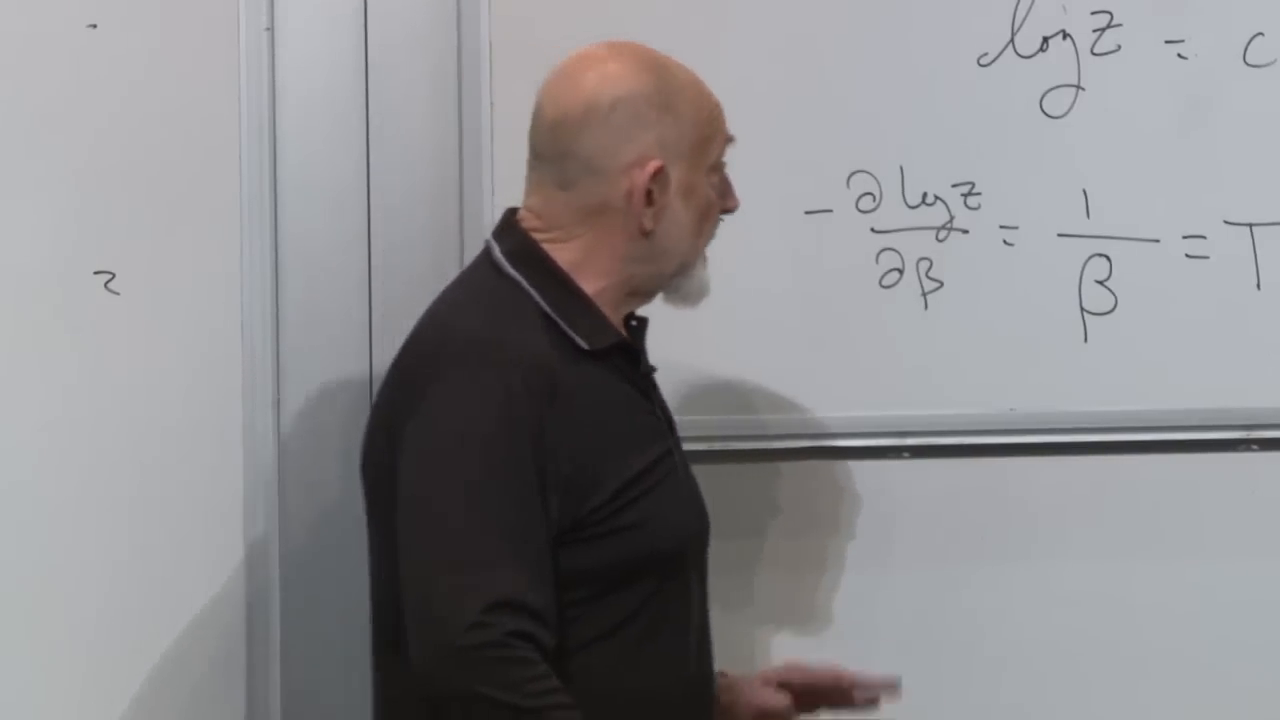
\includegraphics[width=0.90\textwidth]{lecture_07_figure_02.png} \caption{Ước lượng theo tốc độ phân tử, đạo hàm áp suất và phép thế khí lý tưởng được trình bày cùng nhau.} \lectureframe{00:08:55} \end{figure}

Có một sự tinh chỉnh quan trọng. Một sóng âm biên độ nhỏ thông thường nén và làm loãng chất khí nhanh hơn việc nhiệt có thể truyền giữa các phần tử lân cận. Vì vậy, chuyển động cục bộ xấp xỉ đoạn nhiệt chứ không phải đẳng nhiệt: \begin{equation}
 c_s^2=
 \left(\frac{\partial P}{\partial\rho_m}\right)_S.
 \label{eq:sm7-sound-adiabatic}
\end{equation} Đối với một khí lý tưởng có chỉ số đoạn nhiệt \(\gamma\), \begin{equation}
 P\rho_m^{-\gamma}=\text{constant},
 \qquad
 c_s^2=\gamma\frac{P}{\rho_m}
       =\gamma\frac{k_B T}{m}.
 \label{eq:sm7-sound-ideal-adiabatic}
\end{equation} Đối với không khí lưỡng nguyên tử ở nhiệt độ phòng, \(\gamma\simeq 7/5\). Vì thế, phép tính ở nhiệt độ cố định là một ước lượng đầu tiên hữu ích, còn đạo hàm đoạn nhiệt cung cấp sự tinh chỉnh phù hợp về mặt vật lý.

Dùng các giá trị thô \begin{equation}
\begin{aligned}
 k_B&\simeq1.3\times10^{-23}\ {\rm J\,K^{-1}},
 &T&\simeq300\ {\rm K},\\
 m_{\rm air}&\simeq4\times10^{-26}\ {\rm kg}.&&
\end{aligned}
 \label{eq:sm7-air-data}
\end{equation}, ước lượng theo phân tử vào khoảng \(500\ {\rm m\,s^{-1}}\). Ở đây nhiệt độ phải là nhiệt độ tuyệt đối tính bằng kelvin, không phải một thang đo lệch gốc như Fahrenheit. Tốc độ âm thanh quen thuộc có cỡ \(300\ {\rm m\,s^{-1}}\), và công thức khí lý tưởng đoạn nhiệt cho khoảng \(340\ {\rm m\,s^{-1}}\) ở nhiệt độ phòng. Vì vậy, phép tính thô đã tìm ra đúng bậc độ lớn vật lý.

\begin{figure}[t] \centering
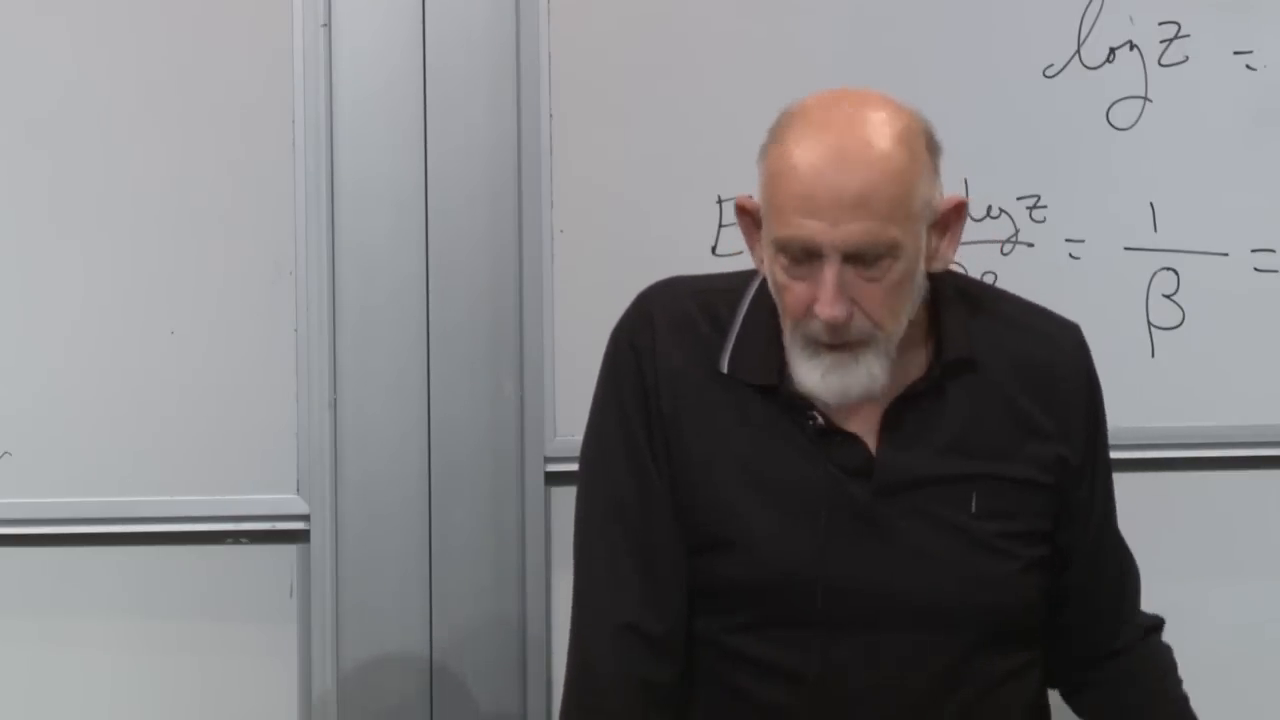
\includegraphics[width=0.90\textwidth]{lecture_07_figure_03.png} \caption{Ước lượng cho không khí ở nhiệt độ phòng dùng hằng số Boltzmann, một khối lượng phân tử hiệu dụng gần \(30\) khối lượng proton, và \(T\simeq300\ {\rm K}\).} \lectureframe{00:10:55} \end{figure}

Từ rất lâu trước khi có được một mô tả vi mô, người ta đã có thể xác định tốc độ âm thanh từ các phép đo áp suất theo khối lượng riêng. Lập luận thống kê bổ sung một cách diễn giải rất đáng chú ý rằng tốc độ vĩ mô ấy được ấn định bởi tốc độ nhiệt của từng phân tử riêng lẻ.

\begin{classroomqa} \audiencequestion{Có cần cộng neutron vào khối lượng phân tử không, và con số \(14\) đối với nitơ có chỉ tính proton thôi không?} \lecturerresponse{Nguyên tử lượng được nêu ra đã tính cả proton lẫn neutron. Phân tử nitơ gồm hai nguyên tử có nguyên tử lượng xấp xỉ \(14\), nên khối lượng của nó xấp xỉ \(28\) khối lượng proton; làm tròn \(28\) thành \(30\) là đủ cho ước lượng này. \lecturetimestamp{00:10:58--00:11:16}} \end{classroomqa}

\begin{classroomqa} \audiencequestion{Hệ số \(3\) xuất phát từ ba phương tịnh tiến, trong khi âm thanh truyền theo một phương. Có phải vì vậy phải bỏ hệ số \(3\) đi không?} \lecturerresponse{Điều đó đúng là nhắc ta không được đồng nhất tốc độ căn trung bình bình phương ba chiều của phân tử với một tốc độ lan truyền một chiều. Lập luận mở đầu chỉ là một bức tranh bậc độ lớn. Câu trả lời chặt chẽ xuất phát từ đạo hàm áp suất, cùng với điều kiện nhiệt động học thích hợp cho sóng. \lecturetimestamp{00:11:12--00:12:00}} \end{classroomqa}

\begin{classroomqa} \audiencequestion{Đạo hàm đó có giả sử rằng nhiệt độ vẫn không đổi trong khi sóng truyền không?} \lecturerresponse{Phép thế khí lý tưởng được trình bày đúng là đã giả sử như vậy. Giữ nhiệt độ cố định là một ước lượng tạm thời hợp lý cho một nhiễu động rất nhỏ; sự tinh chỉnh chuẩn là âm thanh thông thường xấp xỉ đoạn nhiệt, thay đạo hàm đẳng nhiệt bằng \(\left(\partial P/\partial\rho_m\right)_S\). \lecturetimestamp{00:12:59--00:14:01}} \end{classroomqa}

\begin{classroomqa} \audiencequestion{Nếu biến thiên áp suất và khối lượng riêng đều nhỏ, điều đó có làm đạo hàm của chúng nhỏ đi không?} \lecturerresponse{Không. Đạo hàm là tỉ số của hai biến thiên nhỏ trong giới hạn vi phân. Cả \(\delta P\) lẫn \(\delta\rho\) đều có thể nhỏ trong khi \(\delta P/\delta\rho\) vẫn hữu hạn và quyết định tốc độ của sóng. \lecturetimestamp{00:14:03--00:14:23}} \end{classroomqa}

\begin{classroomqa} \audiencequestion{Tốc độ âm thanh có nên tăng khi chất khí bị nén lại, như khi ta đi từ khí về phía lỏng hay rắn không?} \lecturerresponse{Có. Đạo hàm được lấy tại trạng thái đang xét, và \(P(\rho,T)\) không nhất thiết còn tuyến tính. Khi các phân tử bị ép sát nhau, phương trình trạng thái trở nên phi lý tưởng và \(\partial P/\partial\rho\) có thể tăng lên đáng kể. \lecturetimestamp{00:14:25--00:15:13}} \end{classroomqa}

\begin{classroomqa} \audiencequestion{Giá trị \(500\ {\rm m\,s^{-1}}\) có thể dùng ở mọi áp suất không?} \lecturerresponse{Không. Nó thuộc về miền mật độ thấp, nơi phương trình khí lý tưởng là một xấp xỉ hữu ích. Một khi các lũy thừa cao hơn của mật độ đi vào \(P(\rho,T)\), đạo hàm, và do đó tốc độ âm thanh, sẽ phụ thuộc vào áp suất và khối lượng riêng. \lecturetimestamp{00:15:14--00:16:29}} \end{classroomqa}

\begin{classroomqa} \audiencequestion{Bức tranh ban đầu về việc âm thanh lan ra với tốc độ xấp xỉ tốc độ phân tử có cũng thất bại khi mật độ tăng lên không?} \lecturerresponse{Có lẽ có. Bức tranh đó được xây dựng riêng cho chất khí loãng. Ở mật độ cao, các tương tác tập thể trở nên ngày càng quan trọng, và đó chính là lý do đạo hàm của phương trình trạng thái là mô tả tổng quát hơn. \lecturetimestamp{00:16:32--00:16:53}} \end{classroomqa}

\begin{classroomqa} \audiencequestion{Vì sao khối lượng của phân tử nitơ lại được viết là xấp xỉ \(30\) khối lượng proton thay vì \(28\)?} \lecturerresponse{Chỉ cần độ chính xác số phù hợp với phép ước lượng, nên \(28\) đã được làm tròn thành \(30\). Chia ước lượng ban đầu \(500\ {\rm m\,s^{-1}}\) cho \(\sqrt{3}\simeq1.7\) cũng đưa nó lại gần \(300\ {\rm m\,s^{-1}}\), mặc dù đạo hàm đoạn nhiệt mới là cách chặt chẽ để tính hiệu chỉnh đó. \lecturetimestamp{00:16:54--00:17:27}} \end{classroomqa}

\section{Một dao động tử cổ điển trong một bể nhiệt}

Giờ ta thay phân tử chuyển động tịnh tiến tự do bằng một dao động tử điều hòa và coi mọi thứ còn lại là một bể nhiệt. Hình dung trực tiếp là một khối lượng gắn với lò xo, nhưng mô hình này rộng hơn nhiều. Một mốt của khoang điện từ dao động; các nguyên tử trong tinh thể dao động; gần như mọi hệ ổn định bị lệch nhẹ khỏi cân bằng đều thực hiện chuyển động điều hòa ở bậc dẫn đầu.

Với \(x\) được đo từ vị trí cân bằng, xung lượng \(p\), khối lượng \(m\) và hằng số lò xo \(\kappa\), Hamiltonian là \begin{equation}
 H(x,p)=\frac{p^2}{2m}+\frac{\kappa x^2}{2},
 \qquad
 \omega=\sqrt{\frac{\kappa}{m}}.
 \label{eq:sm7-classical-hamiltonian}
\end{equation} Bể nhiệt ấn định \(T\), và từ đây ta lại dùng \(k_B=1\), nên \(\beta=1/T\). Một dao động tử cân bằng nhiệt với phòng có nhiệt độ gần \(300\ {\rm K}\); một dao động tử nhúng trong heli lỏng chỉ có nhiệt độ vài kelvin. Một lò xo giả định đặt ở tâm Mặt Trời sẽ không thể tồn tại như một lò xo, nhưng ví dụ này làm rõ vai trò của môi trường. Trọng số Boltzmann phân tích thành nhân tử: \begin{equation}
 e^{-\beta H}
 =e^{-\beta p^2/(2m)}
  e^{-\beta\kappa x^2/2}.
 \label{eq:sm7-factorized-weight}
\end{equation}

\begin{figure}[t] \centering
\includegraphics[width=0.90\textwidth]{lecture_07_figure_04.png} \caption{Một dao động tử khối lượng-lò xo và Hamiltonian của nó gồm động năng cộng thế năng.} \lectureframe{00:20:55} \end{figure}

Không giống khí tự do, tích phân theo vị trí không chỉ đơn thuần cho ra thể tích của bình chứa. Thế phục hồi gán trọng số cho mỗi li độ:
\begin{equation}
 Z_{\rm cl}
 =\frac{1}{h}\int_{-\infty}^{\infty}dp
             \int_{-\infty}^{\infty}dx\,
 e^{-\beta p^2/(2m)}
 e^{-\beta\kappa x^2/2}.
 \label{eq:sm7-classical-z}
\end{equation}
Thừa số \(1/h\) làm cho hàm phân hoạch cổ điển một chiều trở thành không thứ nguyên. Nó được lược bỏ trong phép tính trên bảng vì không phụ thuộc vào \(\beta\) và không thể ảnh hưởng đến năng lượng trung bình.

\begin{figure}[t]
\centering
\includegraphics[width=0.90\textwidth]{lecture_07_figure_05.png}
\caption{Hàm phân hoạch của dao động tử cổ điển được tách thành các tích phân Gauss theo động lượng và theo li độ.}
\lectureframe{00:22:55}
\end{figure}

Đối với tích phân theo động lượng, đặt
\begin{equation}
 q=\sqrt{\frac{\beta}{2m}}\,p,
 \qquad
 dp=\sqrt{\frac{2m}{\beta}}\,dq.
 \label{eq:sm7-p-gaussian-substitution}
\end{equation}
Đối với tích phân theo vị trí, đặt
\begin{equation}
 y=\sqrt{\frac{\beta\kappa}{2}}\,x,
 \qquad
 dx=\sqrt{\frac{2}{\beta\kappa}}\,dy.
 \label{eq:sm7-x-gaussian-substitution}
\end{equation}
Vì \(\int_{-\infty}^{\infty}e^{-u^2}\,du=\sqrt{\pi}\), tích phân không gian pha không chuẩn hóa được dùng trên bảng là
\begin{equation}
 \int dp\,dx\,e^{-\beta H}
 =\frac{2\pi}{\beta}\sqrt{\frac{m}{\kappa}}
 =\frac{2\pi}{\beta\omega}.
 \label{eq:sm7-classical-z-unnormalized}
\end{equation}
Khi khôi phục ô không gian pha,
\begin{equation}
 Z_{\rm cl}=\frac{2\pi}{h\beta\omega}
           =\frac{1}{\beta\hbar\omega}.
 \label{eq:sm7-classical-z-normalized}
\end{equation}

Đối với năng lượng, chỉ sự phụ thuộc vào \(\beta\) mới quan trọng:
\begin{equation}
 \begin{aligned}
 \log Z_{\rm cl}&=\text{constant}-\log\beta,\\
 \expect{H}
 &=-\frac{\partial\log Z_{\rm cl}}{\partial\beta}\\
 &=\frac{1}{\beta}=T.
 \end{aligned}
 \label{eq:sm7-classical-energy}
\end{equation}

\begin{figure}[t]
\centering
\includegraphics[width=0.90\textwidth]{lecture_07_figure_06.png}
\caption{Chuỗi suy luận cổ điển hoàn chỉnh trên bảng bên phải: phép tách Gauss, \(Z\propto(\beta\omega)^{-1}\), và \(\expect{H}=1/\beta=T\).}
\lectureframe{00:30:15}
\end{figure}

Không có thừa số \(3\) vì đây là một dao động tử trong một chiều không gian. Cũng không còn thừa số \(1/2\) nào nữa, vì có hai hạng bậc hai độc lập. Mỗi tích phân Gauss đóng góp \(T/2\):
\begin{equation}
 \expect{K}=\frac{T}{2},
 \qquad
 \expect{U}=\frac{T}{2},
 \qquad
 \expect{H}=T.
 \label{eq:sm7-equipartition-oscillator}
\end{equation}
Đây là nguyên lý phân bố đều ở dạng hữu ích nhất của nó: mọi hạng bậc hai độc lập trong Hamilton cổ điển đều đóng góp \(T/2\).

Kết quả này không phụ thuộc cả \(m\) lẫn \(\kappa\). Bản thân chuyển động thì có phụ thuộc vào các tham số đó:
\begin{equation}
 \expect{p^2}=mT,
 \qquad
 \expect{x^2}=\frac{T}{\kappa},
 \qquad
 \expect{\dot{x}^2}=\frac{T}{m}.
 \label{eq:sm7-classical-fluctuations}
\end{equation}
Vì vậy, khối lượng lớn hơn chuyển động chậm hơn và lò xo cứng hơn có biên độ nhỏ hơn, mặc dù năng lượng trung bình vẫn là \(T\).
Điều đó trở nên đáng băn khoăn khi \(\kappa\) được làm lớn đến mức phi thường. Một lò xo quá cứng để chuyển động đáng lẽ phải giống như một ràng buộc bị đóng băng, vậy mà phân bố đều cổ điển vẫn gán cho nó năng lượng \(T\).

\begin{classroomqa}
\audiencequestion{Khi \(\kappa\to\infty\), hàm phân hoạch tiến về không. Làm sao vẫn có thể dùng logarit của nó?}
\lecturerresponse{Giữ \(\kappa\) hữu hạn nhưng lớn tùy ý. Đóng góp của nó vào \(\log Z\) là cộng tính và không phụ thuộc vào \(\beta\), nên đạo hàm theo \(\beta\) vẫn cho \(T\). Sự vướng mắc ở giới hạn đó là có thật: phép tính cổ điển là tự nhất quán về nội tại, nhưng nó bỏ sót một đặc điểm của tự nhiên cần thiết cho các dao động tử rất cứng.
\lecturetimestamp{00:34:01--00:34:54}}
\end{classroomqa}

\begin{classroomqa}
\audiencequestion{Hàm phân hoạch của khí lý tưởng cần một \(N!\). Ở đây có nên có một giai thừa tương tự không?}
\lecturerresponse{Không. Ta đang xét một dao động tử được chỉ định cụ thể, chứ không hoán vị \(N\) hạt giống hệt nhau. Đối với nhiều mode độc lập có nhãn, các hàm phân hoạch nhân với nhau. Một thừa số bất khả phân biệt thuộc về một bài toán đếm khác.
\lecturetimestamp{00:35:03--00:35:40}}
\end{classroomqa}

\section{Vì sao nguyên lý phân bố đều cổ điển từng là một cuộc khủng hoảng}

Các phân tử thực không phải là những điểm vô cấu trúc. Một phân tử hai nguyên tử chứa một liên kết có thể dao động, do đó có một dao động tử nội. Một cách đếm cổ điển ngây thơ sẽ gán cho mode đó thêm năng lượng nhiệt ngay cả ở nhiệt độ thông thường. Trong một phép đếm cố ý giản lược, việc kích hoạt một dao động tử dao động nâng năng lượng từ \(3T/2\) lên hướng tới \(5T/2\). Việc hạch toán chính xác nhiệt dung còn phải tính đến các bậc tự do quay và phân biệt năng lượng với đạo hàm của nó theo nhiệt độ. Sự kiện thực nghiệm mang tính quyết định thì đơn giản hơn:
các mode nội cứng đã không đóng góp ở nhiệt độ thấp như phân bố đều cổ điển đòi hỏi.

Ta có thể phủ nhận rằng phân tử có cấu trúc bên trong, điều đó là phi lý, hoặc thừa nhận rằng cơ học cổ điển còn thiếu một thành phần. Thành phần đó là cơ học lượng tử. Ta cần rất ít từ nó: chỉ cần việc một dao động tử điều hòa có các mức năng lượng cách đều.

\section{Dao động tử lượng tử}

Trước hết hãy dịch gốc năng lượng và viết phổ kích thích dưới dạng
\begin{equation}
 E_n^{\rm exc}=n\hbar\omega,
 \qquad n=0,1,2,\ldots.
 \label{eq:sm7-shifted-spectrum}
\end{equation}
Hàm phân hoạch bây giờ là một tổng đúng nghĩa chứ không phải một tích phân trên không gian pha:
\begin{align}
 Z_{\rm exc}
 &=\sum_{n=0}^{\infty}e^{-\beta n\hbar\omega} \notag\\
 &=1+x+x^2+\cdots
  =\frac{1}{1-x},
 \qquad x=e^{-\beta\hbar\omega}, \notag\\
 &=\frac{1}{1-e^{-\beta\hbar\omega}}.
 \label{eq:sm7-quantum-z}
\end{align}

\begin{figure}[t]
\centering
\includegraphics[width=0.90\textwidth]{lecture_07_figure_07.png}
\caption{Các mức cách đều và phép tính hàm phân hoạch của dao động tử lượng tử bằng chuỗi hình học.}
\lectureframe{00:42:05}
\end{figure}

Lấy đạo hàm ta được năng lượng kích thích trung bình:
\begin{align}
 E_{\rm exc}
 &=-\frac{\partial\log Z_{\rm exc}}{\partial\beta}
  =-\frac{1}{Z_{\rm exc}}
    \frac{\partial Z_{\rm exc}}{\partial\beta}
 \notag\\
 &=\hbar\omega\,
   \frac{e^{-\beta\hbar\omega}}
        {1-e^{-\beta\hbar\omega}}
  =\frac{\hbar\omega}{e^{\beta\hbar\omega}-1}.
 \label{eq:sm7-quantum-energy}
\end{align}

\begin{figure}[t]
\centering
\includegraphics[width=0.90\textwidth]{lecture_07_figure_08.png}
\caption{Năng lượng kích thích nhiệt thu được từ đạo hàm theo \(\beta\) của hàm phân hoạch lượng tử.}
\lectureframe{00:46:05}
\end{figure}

\subsection{Nhiệt độ cao}

Khi \(\beta\hbar\omega\ll1\),
\begin{equation}
 e^{-\beta\hbar\omega}
 =1-\beta\hbar\omega
  +O\!\left((\beta\hbar\omega)^2\right).
 \label{eq:sm7-high-t-expansion}
\end{equation}
Tử số của \eqref{eq:sm7-quantum-energy} tiến tới \(\hbar\omega\), còn mẫu số, ở bậc dẫn đầu, là \(\beta\hbar\omega\). Vì vậy
\begin{equation}
 E_{\rm exc}\simeq\frac{1}{\beta}=T.
 \label{eq:sm7-high-t-energy}
\end{equation}
Kết quả lượng tử khôi phục nguyên lý phân bố đều cổ điển khi nhiều khoảng cách mức nằm trong năng lượng nhiệt.

\subsection{Nhiệt độ thấp}

Khi \(\beta\hbar\omega\gg1\), số mũ là rất nhỏ:
\begin{equation}
 E_{\rm exc}
 \simeq\hbar\omega e^{-\beta\hbar\omega}.
 \label{eq:sm7-low-t-energy}
\end{equation}
Kích thích nhiệt của dao động tử bị suy giảm theo hàm mũ. Trong quy ước đã dịch gốc, nó gần như bằng không; năng lượng điểm không của hệ theo nghĩa vật lý sẽ được phục hồi ở dưới.

\begin{figure}[t]
\centering
\includegraphics[width=0.90\textwidth]{lecture_07_figure_09.png}
\caption{Khai triển ở nhiệt độ thấp: kích thích nhiệt đầu tiên bị suy giảm bởi \(e^{-\beta\hbar\omega}\).}
\lectureframe{00:51:55}
\end{figure}

Sự chuyển tiếp xảy ra khi
\begin{equation}
 \beta\hbar\omega\sim1,
 \qquad\text{or equivalently}\qquad
 T\sim\hbar\omega.
 \label{eq:sm7-crossover}
\end{equation}
Điều kiện này có một ý nghĩa trực tiếp. Phân bố đều cổ điển sẽ cho năng lượng dao động tử bằng \(T\). Các hiệu ứng lượng tử trở nên không thể tránh khỏi khi thang đó nhỏ hơn một khoảng cách mức. Vì vậy
\begin{equation}
\begin{aligned}
 \hbar\omega\gg T&:\quad \text{frozen and quantum},\\
 \hbar\omega\ll T&:\quad \text{active and classical}.
\end{aligned}
 \label{eq:sm7-regimes}
\end{equation}
Một lò xo cứng hơn có \(\omega=\sqrt{\kappa/m}\) lớn hơn, nên nó đòi hỏi nhiệt độ cao hơn trước khi ứng xử cổ điển.

\section{Các bậc tự do xuất hiện khi ta nung nóng vật chất}

Ở nhiệt độ thấp, một phân tử hai nguyên tử về mặt nhiệt có thể giống một hạt điểm vì dao động liên kết cứng của nó bị đóng băng. Khi \(T\) tăng vượt \(\hbar\omega\), mode dao động được kích hoạt. Các mode quay có thể được kích hoạt ở một thang thấp hơn; ở nhiệt độ còn cao hơn nữa, nhiều chuyển động bên trong hơn lộ ra và cuối cùng nguyên tử bị ion hóa. Sự nung nóng không chỉ đơn thuần đưa nhiều năng lượng hơn vào một danh sách mode cố định. Nó làm lộ ra những bậc tự do vốn vô hình ở nhiệt độ thấp hơn.

Một phân tử lồng nhau tưởng tượng làm rõ hơn luận điểm này. Hai nguyên tử được nối với nhau bằng một lò xo cứng, trong khi một nguyên tử biểu kiến tự nó lại là một cặp được nối bằng một lò xo còn cứng hơn nữa. Ở \(T\) thấp, cả hai cấu trúc đều trông như hạt điểm. Ở ngưỡng thứ nhất, dao động bên ngoài xuất hiện; ở ngưỡng thứ hai, cấu trúc bên trong xuất hiện. Độ phức tạp của hệ được bộc lộ từng thang năng lượng một.

\begin{classroomqa}
\audiencequestion{Khi một dao động tử đã ở trong miền cổ điển rồi, việc tiếp tục nung nóng có làm lò xo cứng hơn hoặc làm thay đổi tần số của nó không?}
\lecturerresponse{Không. Hằng số lò xo và tần số vẫn giữ cố định. Nhiệt độ cao hơn tạo ra các động lượng và biên độ điển hình lớn hơn, do đó năng lượng lớn hơn. Độ cứng quyết định nhiệt độ mà tại đó định luật cổ điển bắt đầu có hiệu lực, chứ không phải sự cứng lên của lò xo phụ thuộc vào nhiệt độ.
\lecturetimestamp{01:03:17--01:05:11}}
\end{classroomqa}

\subsection{Tinh thể và nhiệt dung riêng của Einstein}

Một tinh thể chứa rất nhiều mode dao động. Phân bố đều cổ điển gán năng lượng cỡ \(T\) cho mọi dao động tử đang hoạt động và vì thế đánh giá quá cao nhiệt dung ở nhiệt độ thấp. Mô hình 1907 của Einstein xử lý các dao động tinh thể bằng cơ học lượng tử và chỉ ra vì sao chúng bị suy giảm cho đến khi năng lượng nhiệt đạt tới khoảng cách mức của chúng. Các mô hình chất rắn chính xác hơn cho phép một phân bố tần số mode, nhưng nguyên lý đóng băng đã có mặt ngay trong phép tính của Einstein.

\begin{classroomqa}
\audiencequestion{Đây có phải là công trình mà Einstein nhận giải Nobel hay không, và nó chỉ xuất hiện sau khi cơ học lượng tử đã được thiết lập hay sao?}
\lecturerresponse{Không. Trích dẫn của giải Nobel liên quan đến hiệu ứng quang điện. Mô hình nhiệt dung riêng được công bố vào 1907, rất lâu trước khi những nền tảng đầy đủ của cơ học lượng tử được hiểu rõ. Einstein đã chấp nhận và phát triển những ý tưởng lượng tử then chốt, dù về sau ông phản đối một số khía cạnh của lý thuyết ở dạng hoàn chỉnh.
\lecturetimestamp{00:58:38--01:03:16}}
\end{classroomqa}

\begin{classroomqa}
\audiencequestion{Cơ học thống kê cổ điển đã thay một tổng trên các trạng thái rời rạc bằng một tích phân dường như đồng đều trên vị trí và động lượng. Điều gì biện minh cho phép đếm trạng thái đó?}
\lecturerresponse{Sự biện minh rốt cuộc đến từ cơ học lượng tử. Trong giới hạn nhiệt độ cao,
\[
 Z_{\rm exc}\simeq\frac{1}{\beta\hbar\omega},
\]
điều này khớp chính xác với kết quả cổ điển không thứ nguyên \eqref{eq:sm7-classical-z-normalized}. Các ô lượng tử trong không gian pha trở thành độ đo không gian pha cổ điển khi khoảng cách mức không còn được phân giải.
\lecturetimestamp{00:59:38--01:03:06}}
\end{classroomqa}

\subsection{Một dây chứa vô hạn nhiều dao động tử}

Một dây đàn violin hay guitar phân rã thành các mode chuẩn: mode cơ bản, các họa âm bậc cao hơn, và các bước sóng ngày càng ngắn hơn. Về mặt toán học có vô hạn mode dao động. Nếu nguyên lý phân bố đều cổ điển gán năng lượng \(T\) cho mỗi mode, thì sợi dây ở cân bằng nhiệt sẽ có năng lượng vô hạn. Cơ học lượng tử ngăn thảm họa đó xảy ra. Các mode có bước sóng ngắn nhất có tần số cao nhất và bị đóng băng ở mọi nhiệt độ hữu hạn; khi \(T\) tăng lên thì ngày càng nhiều mode được kích hoạt. Lập luận tương tự về sau cũng sẽ là cơ sở của bức xạ vật đen.

\begin{figure}[t]
\centering
\includegraphics[width=0.90\textwidth]{lecture_07_figure_10.png}
\caption{Một số mode chuẩn chồng chập trên một sợi dây, minh họa vì sao một sợi dây liên tục là một tập hợp vô hạn các dao động tử điều hòa.}
\lectureframe{01:09:30}
\end{figure}

\begin{classroomqa}
\audiencequestion{Có thể quan sát trực tiếp sự chuyển tiếp từ lượng tử sang cổ điển không, và việc nung nóng có thể đảo ngược hành vi ở nhiệt độ thấp không?}
\lecturerresponse{Có. Sự phụ thuộc vào nhiệt độ của nhiệt dung riêng của một tinh thể khiến sự đóng băng và sự kích hoạt tiếp theo của các mode dao động trở nên đo được một cách rõ ràng.
\lecturetimestamp{01:09:11--01:10:13}}
\end{classroomqa}

\begin{classroomqa}
\audiencequestion{Đối với nhiều dao động tử, ta có lặp lại hàm phân hoạch của một dao động tử đơn cho từng mode không?}
\lecturerresponse{Đối với các mode độc lập,
\[
\begin{aligned}
 Z_{\rm tot}&=\prod_j Z_j,&
 \log Z_{\rm tot}&=\sum_j\log Z_j,\\
 E_{\rm tot}&=\sum_j E_j.&&
\end{aligned}
\]
Các mode với \(\hbar\omega_j\gg T\) cho đóng góp nhiệt nhỏ theo hàm mũ; những mode nằm dưới ngưỡng thì đóng góp đáng kể.
\lecturetimestamp{01:10:14--01:11:00}}
\end{classroomqa}

\begin{classroomqa}
\audiencequestion{Năng lượng điểm không của dao động tử \(\hbar\omega/2\) đã đi đâu?}
\lecturerresponse{Các mức năng lượng vật lý là
\[
 E_n=\left(n+\frac12\right)\hbar\omega.
\]
Do đó
\[
 \begin{aligned}
 Z_{\rm phys}
 &=e^{-\beta\hbar\omega/2}Z_{\rm exc},\\
 E_{\rm phys}
 &=\frac{\hbar\omega}{2}
  +\frac{\hbar\omega}{e^{\beta\hbar\omega}-1}.
 \end{aligned}
\]
Độ dời chung ấy không làm thay đổi các xác suất mức, entropy, nhiệt dung, hay năng lượng kích thích nhiệt, nhưng nó làm dời giá trị trung bình tuyệt đối của năng lượng đi một lượng \(\hbar\omega/2\). Thừa số nhân trong \(Z\) phụ thuộc vào \(\beta\), vì vậy không được bỏ nó đi khi cần năng lượng tuyệt đối.
\lecturetimestamp{01:11:08--01:11:37}}
\end{classroomqa}

\section{Định luật thứ hai như một bài toán về tính thuận nghịch}

Bây giờ ta có thể quay lại vấn đề đã hứa. Định luật thứ hai nói rằng sự tiến hóa vĩ mô thông thường là không thuận nghịch và entropy có xu hướng tăng. Sự tiến hóa Hamilton vi mô là thuận nghịch. Làm sao một ánh xạ thuận nghịch của các trạng thái chính xác lại có thể tạo ra một định luật không thuận nghịch cho các trạng thái vĩ mô?

Biểu diễn hệ bằng một điểm trong không gian pha nhiều chiều,
\[
 \Gamma=(q_1,\ldots,q_N,p_1,\ldots,p_N).
\]
Kiến thức của ta thường không phải là một điểm chính xác. Giả sử nó là một mật độ xác suất đều trên một miền compact \(A\) có thể tích \(\Omega_A\):
\begin{equation}
 f(\Gamma)=
 \begin{cases}
  1/\Omega_A,&\Gamma\in A,\\
  0,&\Gamma\notin A.
 \end{cases}
 \label{eq:sm7-uniform-blob}
\end{equation}
Trong hệ đơn vị với \(k_B=1\), entropy Gibbs hạt mịn của nó là
\begin{equation}
 S_{\rm fine}
 =-\int d\Gamma\,f\log f
 =\log\Omega_A.
 \label{eq:sm7-blob-entropy}
\end{equation}
Một miền nhỏ hơn có nghĩa là nhiều thông tin hơn và entropy thấp hơn. Điều này ấn định dấu: độ bất định tăng lên làm miền bị chiếm mở rộng ra và làm tăng \(\log\Omega_A\).

\begin{figure}[t]
\centering
\includegraphics[width=0.90\textwidth]{lecture_07_figure_11.png}
\caption{Một miền xác suất compact trong một lát cắt hai chiều mang tính sơ đồ của toàn bộ không gian pha vị trí-xung lượng.}
\lectureframe{01:20:20}
\end{figure}

\begin{classroomqa}
\audiencequestion{Hệ có bị ràng buộc vật lý phải ở trong miền đã vẽ hay không, và nó đã ở cân bằng hay chưa?}
\lecturerresponse{Không. Miền đó mô tả những gì được biết về trạng thái ban đầu, chứ không phải một bức tường trong không gian pha. Nó không nhất thiết là một phân bố cân bằng. Một chất khí ban đầu bị giam trong một bình chứa ở một góc phòng là một ví dụ cụ thể về thông tin đặc biệt, không cân bằng.
\lecturetimestamp{01:14:55--01:15:24}}
\end{classroomqa}

\section{Dòng chảy Liouville và sự tăng khi làm thô}

Định lý Liouville nói rằng dòng Hamilton bảo toàn thể tích không gian pha. Miền chính xác có thể tịnh tiến, kéo dãn, gấp nếp và trở nên cực kỳ mảnh, nhưng
\begin{equation}
 \Omega_{A(t)}=\Omega_{A(0)},
 \qquad
 S_{\rm fine}(t)=S_{\rm fine}(0).
 \label{eq:sm7-liouville}
\end{equation}
Tương tự rời rạc là một phép hoán vị thuận nghịch của các trạng thái. Nếu ban đầu ta biết rằng một con xúc xắc nằm trong một trong hai trạng thái, thì một sự tiến hóa một-một có thể làm thay đổi đó là hai trạng thái nào, nhưng không làm thay đổi số khả năng.

Những mô tả thực tế có độ phân giải hữu hạn. Cơ học lượng tử cung cấp một ô không gian pha tự nhiên, trong khi ngay cả một thí nghiệm cổ điển cũng có năng lực đo hữu hạn mà không cần viện đến lý thuyết lượng tử. Dưới dòng Hamilton, miền đó có thể biến thành một dải dài, mảnh như con rắn. Nếu khoảng cách giữa các nếp gấp lân cận của nó giảm xuống dưới thang độ phân giải, ta thay mỗi lân vực không còn phân giải được bằng một ô thô. Thể tích bị chiếm chính xác vẫn giữ nguyên, nhưng hợp của các ô thô thì tăng lên:
\begin{equation}
 \Omega_{\rm coarse}(t)\geq\Omega_{A(t)},
 \qquad
 S_{\rm coarse}(t)=\log\Omega_{\rm coarse}(t).
 \label{eq:sm7-coarse-entropy}
\end{equation}

\begin{figure}[t]
\centering
\includegraphics[width=0.90\textwidth]{lecture_07_figure_12.png}
\caption{Một sợi mảnh bảo toàn thể tích được quan sát qua các ô có độ phân giải hữu hạn. Sợi đen chính xác giữ nguyên diện tích của nó; các ô thô màu đỏ chiếm một miền hiệu dụng lớn hơn.}
\lectureframe{01:22:10}
\end{figure}

\begin{classroomqa}
\audiencequestion{Các ô thô chồng lấn lên nhau. Điều đó có vi phạm định lý Liouville không?}
\lecturerresponse{Không. Định lý Liouville chi phối sợi mảnh chính xác, vốn vẫn là một ánh xạ một-một và bảo toàn thể tích. Sự chồng lấn thuộc về mô tả bị làm mờ của ta: ta đã vứt bỏ thông tin về việc trạng thái nằm trong nhánh mảnh nào.
\lecturetimestamp{01:21:32--01:21:50}}
\end{classroomqa}

Một phép loại suy hữu ích là bông. Thể tích vật chất của toàn bộ các sợi có thể gần như không đổi, trong khi một búi bông bị tơi ra lại chiếm một thể tích biểu kiến lớn đối với người quan sát không thể phân giải từng sợi riêng lẻ. Tương tự, một miền trong không gian pha mọc ra các tua ngày càng mảnh; rồi chính các tua đó lại phát triển những tua còn mảnh hơn nữa. Bất kỳ độ phân giải hữu hạn cố định nào cuối cùng cũng không theo kịp chúng.

\begin{classroomqa}
\audiencequestion{Có phải entropy chỉ có vẻ tăng trong cơ học cổ điển, còn cơ học lượng tử làm cho sự tăng ấy trở thành thật bằng cách áp đặt một giới hạn độ phân giải cơ bản không?}
\lecturerresponse{Lập luận làm thô không đòi hỏi một giới hạn lượng tử. Entropy đồng thời quy chiếu tới hệ và những phân biệt vĩ mô được giữ lại trong mô tả của nó. Với thông tin vi mô vô hạn, entropy hạt mịn là hằng số; với bất kỳ độ phân giải hữu hạn cố định nào, các sợi mảnh hỗn loạn rốt cuộc trở nên không còn phân giải được và entropy hạt thô tăng lên.
\lecturetimestamp{01:24:04--01:25:20}}
\end{classroomqa}

\section{Hỗn loạn, miền khả đạt hữu hạn, và sự cân bằng hóa}

Đối với một chất khí trong hộp, các vị trí là bị chặn. Ở tổng năng lượng hữu hạn cố định, các xung lượng cũng bị chặn, ngay cả khi toàn bộ năng lượng tạm thời tập trung vào một hạt. Vì vậy, vỏ năng lượng khả đạt về mặt động lực có độ đo hữu hạn dưới các giả thiết giam giữ thông thường.

\begin{figure}[t]
\centering
\includegraphics[width=0.90\textwidth]{lecture_07_figure_13.png}
\caption{Một miền không gian pha khả đạt bị chặn đặt cạnh sợi mảnh và biểu diễn hạt thô của nó.}
\lectureframe{01:28:10}
\end{figure}

Các điểm ban đầu gần nhau trong một hệ hỗn loạn sẽ đi theo những lịch sử tương tự nhau trong một thời gian rồi tách ra. Trong một cú phát bi-a, một thay đổi không thể nhận ra trong hướng của bi cái được truyền vào các va chạm về sau; các khác biệt chồng chất lên nhau cho đến khi các cấu hình cuối cùng không còn liên hệ. Vì thế, cả một miền ban đầu bị kéo dãn và gấp nếp khắp miền khả đạt. Ở độ phân giải hữu hạn, nó tiến gần tới một mô tả cân bằng rộng, gần như đồng đều.

\begin{figure}[t]
\centering
\includegraphics[width=0.90\textwidth]{lecture_07_figure_14.png}
\caption{Một trạng thái đặc biệt compact tiến hóa thành một sợi mảnh phức tạp xuyên khắp miền khả đạt bị chặn, trong khi các ô hạt thô lan ra trên một vùng lớn hơn nhiều.}
\lectureframe{01:33:10}
\end{figure}

Hai điều cần lưu ý là quan trọng. Bản thân hỗn loạn không tự nó chứng minh rằng mọi quỹ đạo đều đi qua mọi lân vực khả đạt; khẳng định lấy mẫu mạnh hơn đó đòi hỏi tính ergodic hoặc tính trộn. Cũng không phải mọi hệ vật lý đều hỗn loạn. Một chất khí nhiều hạt điển hình và các hệ bi-a lý tưởng hóa cung cấp bối cảnh được nhắm tới, nơi tính trộn là một kỳ vọng vật lý hữu ích.

\section{Hồi quy không xóa bỏ tính không thuận nghịch}

Giả sử tất cả các phân tử không khí ban đầu ở một góc với một mẫu vận tốc được chuẩn bị đặc biệt. Các va chạm nhanh chóng làm chúng lan khắp căn phòng, và mô tả hạt thô đạt tới cân bằng. Trong một không gian pha bảo toàn độ đo hữu hạn, định lý hồi quy Poincaré nói rằng hầu như mọi điểm ban đầu đều quay trở lại gần tùy ý điểm xuất phát của nó. Với một dung sai \(\epsilon>0\), một thời gian hồi quy \(t_R(\epsilon)\) là hữu hạn dưới các giả thiết của định lý, mặc dù đối với một hệ vĩ mô thì nó lớn đến khó tin. Sự quay lại chính xác tới một điểm chính xác vô hạn không phải là điều được đòi hỏi, cũng không phải điều nhìn chung được mong đợi.

\begin{classroomqa}
\audiencequestion{Trong ví dụ bi-a, việc đánh vào bi cái có bơm năng lượng vào và làm hỏng sự tiến hóa kín không?}
\lecturerresponse{Trạng thái ban đầu được chọn là trạng thái ngay sau cú đánh, khi năng lượng đó đã được tính vào rồi. Hồi quy liên quan đến động lực học bi-a lý tưởng hóa, cô lập diễn ra sau đó; một lần quay lại gần trạng thái ban đầu bao hàm một cấu hình tương đương với việc bi cái tiến gần cụm bi trong phạm vi dung sai đã chọn.
\lecturetimestamp{01:35:37--01:35:55}}
\end{classroomqa}

\begin{classroomqa}
\audiencequestion{Nếu chất khí rốt cuộc có thể trở lại góc phòng, thì ta có mất thông tin không, và hệ có thực sự thuận nghịch không?}
\lecturerresponse{Động lực học vi mô vẫn thuận nghịch trong suốt quá trình. Entropy hạt thô có thể tăng vì ta thôi không còn phân giải các tương quan tinh vi, nhưng một thăng giáng cực kỳ hiếm vẫn có thể đưa hệ trở lại gần trạng thái vĩ mô ban đầu đặc biệt của nó. Vì vậy, hồi quy và tính không thuận nghịch hạt thô là tương thích với nhau.
\lecturetimestamp{01:37:34--01:38:15}}
\end{classroomqa}

Điều này dẫn tới cách phát biểu cốt yếu của Boltzmann. Entropy không tăng ở mọi khoảnh khắc khả dĩ về mặt logic. Xuất phát từ một trạng thái vĩ mô không cân bằng của một hệ lớn, có áp đảo nhiều diễn biến vi mô tiếp theo tương thích dẫn tới những trạng thái vĩ mô lớn hơn, thay vì tới những trạng thái còn đặc biệt hơn nữa. Entropy \emph{có lẽ} tăng. Các thăng giáng đi xuống và các sự hồi quy đều được phép, nhưng xác suất và thang thời gian của chúng khiến chúng trở nên vô hình trong kinh nghiệm vĩ mô thông thường. Vấn đề tính thuận nghịch là một trong những cuộc đấu tranh lịch sử lớn của cơ học thống kê và đè nặng lên Boltzmann. Mối liên hệ lịch sử đó không nên bị biến thành một khẳng định nhân quả đơn giản về cuộc đời ông.

\section{Hỗn loạn có nghĩa là gì}

Để có một định nghĩa mang tính thao tác hơn về hỗn loạn, giả sử hai điểm pha ban đầu sai khác nhau một lượng \(\delta\Gamma(0)\); theo một hướng hỗn loạn, điển hình ta có
\begin{equation}
 \lVert\delta\Gamma(t)\rVert
 \sim e^{\lambda t}\lVert\delta\Gamma(0)\rVert,
 \qquad \lambda>0,
 \label{eq:sm7-lyapunov-growth}
\end{equation}
trong miền mà xấp xỉ tuyến tính cho sự tách biệt còn có ý nghĩa. Đại lượng \(\lambda\) là một số mũ Lyapunov. Để dự đoán tại thời điểm \(t\), độ chính xác cần có của dữ liệu ban đầu tỉ lệ gần đúng như \(e^{-\lambda t}\). Độ chính xác của quy luật động lực học cũng quan trọng: các sai số mô hình được khuếch đại cùng với các sai số trong điều kiện ban đầu. Thời tiết là ví dụ quen thuộc.

\begin{classroomqa}
\audiencequestion{Có nguyên lý nào nói rằng \emph{đa số} các hệ là hỗn loạn, hay điều đó chỉ đơn thuần là một nhận định thực nghiệm?}
\lecturerresponse{Có vô hạn Hamiltonian hỗn loạn và không hỗn loạn, và ngay cả khái niệm \emph{đa số} cũng đòi hỏi một độ đo trên không gian các Hamiltonian. Các hệ tương tác phức tạp thường là hỗn loạn, nhưng không có phép kiểm tra phổ quát đơn giản nào có thể phân loại mọi Hamiltonian chỉ bằng xem xét trực tiếp.
\lecturetimestamp{01:39:27--01:40:49}}
\end{classroomqa}

\begin{classroomqa}
\audiencequestion{Chính xác thì \emph{hỗn loạn} có nghĩa gì trong thảo luận này?}
\lecturerresponse{Các quỹ đạo pha lân cận tách ra đủ nhanh để việc dự đoán trong thời gian dài đòi hỏi hiểu biết về điều kiện ban đầu phải được cải thiện theo hàm mũ. Bộ dao động điều hòa là trường hợp đối lập: các điểm pha lân cận quay cùng nhau và vẫn ở gần nhau. Bài toán Kepler hai vật chính xác cũng không hỗn loạn, trong khi bài toán ba vật tổng quát có các chế độ hỗn loạn.
\lecturetimestamp{01:40:50--01:43:45}}
\end{classroomqa}

\begin{classroomqa}
\audiencequestion{Các định luật chuyển động, cũng như các điều kiện ban đầu, có phải đều cần được biết với độ chính xác cao không?}
\lecturerresponse{Có. Cả hai nguồn sai số đều lan truyền qua động lực học, và sự tiến hóa hỗn loạn khuếch đại cả hai.
\lecturetimestamp{01:43:46--01:43:55}}
\end{classroomqa}

Con lắc kép cung cấp một ví dụ sinh động. Một con lắc thông thường là khả tích và có thể dự đoán được. Thêm một con lắc thứ hai, và các quỹ đạo khởi đầu gần như cùng nhau về sau có thể trao đổi năng lượng theo những cách khác nhau và đi theo những hướng hoàn toàn khác nhau.

\begin{figure}[t]
\centering
\includegraphics[width=0.90\textwidth]{lecture_07_figure_15.png}
\caption{Con lắc kép như một ví dụ cụ thể về hỗn loạn xác định.}
\lectureframe{01:44:40}
\end{figure}

\begin{classroomqa}
\audiencequestion{Vì sao một hệ cơ học có thể hỗn loạn còn một hệ khác thì không?}
\lecturerresponse{Đó là một tính chất của Hamiltonian và các cấu trúc bất biến của nó, chứ không phải hệ quả của ma sát hay nhiễu thực nghiệm. Việc xác định điều đó có thể khó về mặt toán học; tính phức tạp là dấu hiệu gợi ý chứ không phải bằng chứng.
\lecturetimestamp{01:44:03--01:45:58}}
\end{classroomqa}

\begin{classroomqa}
\audiencequestion{Một con lắc kép lý tưởng, không có ma sát, vẫn hỗn loạn chứ?}
\lecturerresponse{Có. Không cần sự tiêu tán. Chuyển động Hamilton xác định chính xác có thể có sự phụ thuộc nhạy vào điều kiện ban đầu. Dữ liệu ban đầu với độ chính xác vô hạn sẽ xác định quỹ đạo vô thời hạn, nhưng độ chính xác hữu hạn cho một chân trời dự đoán hữu hạn.
\lecturetimestamp{01:45:57--01:47:54}}
\end{classroomqa}

\begin{classroomqa}
\audiencequestion{Hỗn loạn có đồng nghĩa với việc không có nghiệm dạng đóng không?}
\lecturerresponse{Không. Các hệ hỗn loạn nói chung thiếu một quỹ đạo dạng đóng hữu ích trên toàn cục, nhưng khả giải giải tích và sự phụ thuộc nhạy là những tính chất khác nhau. Hỗn loạn được chẩn đoán về mặt động lực học qua sự tách rời của các quỹ đạo, chứ không chỉ bởi việc ta không thể viết ra một công thức.
\lecturetimestamp{01:48:20--01:49:23}}
\end{classroomqa}

\begin{classroomqa}
\audiencequestion{Hỗn loạn lan tỏa khác với việc cân bằng đúng tại đỉnh không ổn định của một ngọn đồi như thế nào?}
\lecturerresponse{Đỉnh đồi là một trạng thái không ổn định ngoại lệ: rời khỏi nó, các quỹ đạo lân cận không nhất thiết tách ra nhanh. Trong một vùng hỗn loạn, tính không ổn định là điển hình dọc theo quỹ đạo và các điểm pha lân cận lặp đi lặp lại tách xa nhau. Một số mũ Lyapunov dương đặc trưng cho sự tăng trưởng bền bỉ đó.
\lecturetimestamp{01:49:27--01:50:11}}
\end{classroomqa}

\section{Từ chuyển động vi mô đến định luật thống kê}

Ước lượng tốc độ âm cho thấy chuyển động nhiệt vi mô ấn định một thang truyền lan vĩ mô như thế nào, trong khi các câu hỏi làm lộ rõ đạo hàm nhiệt động lực học nào phải được chỉ rõ. Bộ dao động sau đó cho thấy cả phạm vi áp dụng lẫn sự thất bại của nguyên lý phân bố đều năng lượng cổ điển. Khoảng cách giữa các mức lượng tử làm đóng băng các mode cứng, giải thích vì sao nhiệt dung thay đổi theo nhiệt độ, và ngăn không cho vô hạn nhiều mode tần số cao mang năng lượng nhiệt vô hạn.

Cũng chính tiến trình từ vi vật lý chính xác đến mô tả vĩ mô hiệu dụng đó giải quyết mâu thuẫn bề ngoài ở cốt lõi của định luật thứ hai. Dòng chảy Hamiltonian bảo toàn chính xác thể tích không gian pha và vẫn thuận nghịch. Sự kéo giãn hỗn loạn tạo ra những tương quan tinh hơn mức mà mô tả vĩ mô còn giữ lại, nên miền bị chiếm sau khi làm thô tăng lên. Tính hồi quy bảo đảm rằng những sự quay trở lại hiếm hoi không bị cấm; xác suất giải thích vì sao chúng không đặc trưng cho kinh nghiệm thông thường. Định luật thứ hai không phải là một lực vi mô không thuận nghịch mới. Nó là hướng tiến hóa thống kê có độ tin cậy áp đảo đối với các điều kiện ban đầu vĩ mô đặc biệt trong những hệ có số bậc tự do cực lớn.
\chapter{Hồi quy, trật tự phi cân bằng và các spin Ising}

\lectureoverview{Một chất khí được giải phóng từ một nửa căn phòng lao nhanh tới cân bằng, nhưng cơ học thuận nghịch nói rằng sự tiến hóa đủ dài cũng tất phải tạo ra những lần trở lại trạng thái ngoại lệ. Chúng ta ước tính thời gian trở lại đó từ thể tích không gian pha, tách hiện tượng hồi quy khỏi sự khởi đầu entropy thấp của vũ trụ mà ta vẫn chưa giải thích được, và dùng nghịch lý nảy sinh từ đó để bàn về các bộ não Boltzmann, lịch sử mạch lạc, và sự sống được duy trì bởi một dòng năng lượng. Sau đó ta chuyển sang trật tự từ. Các spin hai trạng thái độc lập cho ta một bài khởi động giải được chính xác: tổ hợp học quyết định hàm phân hoạch và độ từ hóa là hàm tang hyperbol. Tương tác láng giềng cuối cùng khôi phục một đối xứng lên--xuống và dẫn tới mô hình Ising một chiều.}

\section{Không khí trong một căn phòng rốt cuộc sẽ quay trở lại}

Hãy bắt đầu với toàn bộ không khí ở nửa bên trái của một căn phòng. Có thể chuẩn bị trạng thái này bằng một vách ngăn: hút hết không khí ở nửa phải, đặt không khí ở bên trái, rồi dỡ vách đi. Chất khí lan nhanh khắp căn phòng và tiến gần tới cân bằng nhiệt. Entropy tăng. Không có gì đáng ngạc nhiên đã xảy ra.

Bây giờ hãy để căn phòng kín lại và chờ. Một triệu lần ngửa liên tiếp là một chuỗi kết quả tung đồng xu cực kỳ khó xảy ra, nhưng một thí nghiệm lặp đi lặp lại vô thời hạn rốt cuộc cũng tạo ra những chuỗi cực kỳ khó xảy ra. Cùng một logic ấy áp dụng cho chất khí. Vào một thời điểm xa xôi nào đó, tất cả các phân tử của nó sẽ lại được tìm thấy trong nửa bên trái, hoặc trong một miền đặc biệt tương tự nào đó. Một sự trở lại như vậy là một hồi quy Poincaré.

Định lý chính xác cẩn trọng hơn bức tranh này đôi chút. Đối với một miền có độ đo hữu hạn của không gian pha mà động lực học của nó bảo toàn thể tích không gian pha, hầu như mọi điểm ban đầu đều quay trở lại gần điểm xuất phát của nó đến mức tùy ý. Một phát biểu vĩ mô như \emph{mọi phân tử đều ở nửa bên trái} thì dễ hơn: nó chỉ đòi hỏi quỹ đạo đi vào lại một miền hữu hạn đã làm thô, chứ không phải mọi tọa độ phân tử đều quay về chính xác. Câu hỏi thực tế là việc đó mất bao lâu.

\subsection{Một điểm pha nhiều chiều}

Đối với \(N\) hạt cổ điển, không gian pha có \(6N\) tọa độ,
\begin{equation}
 \Gamma=(\bm x_1,\ldots,\bm x_N;\bm p_1,\ldots,\bm p_N).
 \label{eq:sm8-phase-point}
\end{equation}
Các vị trí bị giới hạn bởi căn phòng. Ở tổng năng lượng cố định, các động lượng cũng bị chặn, bởi vì một hạt không thể mang động lượng lớn tùy ý mà không đồng thời mang năng lượng lớn tùy ý. Vì thế, dưới các giả thiết của lập luận về hồi quy, vỏ năng lượng được phép có độ đo hữu hạn.

Điểm pha chuyển động một cách tất định, nhưng trong một chất khí nhiều hạt thì chuyển động của nó là hỗn loạn. Các quỹ đạo gần nhau tách xa nhau nhanh chóng, như trong một chuỗi va chạm bi-a. Sau khi làm thô, một quỹ đạo dài dường như lang thang khắp miền khả dĩ.

\begin{figure}[t]
\centering
\includegraphics[width=0.90\textwidth]{lecture_08_figure_02.png}
\caption{Một miền không gian pha minh họa và một quỹ đạo phức tạp lang thang trong đó. Hình vẽ cố ý có số chiều thấp; chất khí thật sự sống trong một không gian \(6N\) chiều.}
\lectureframe{00:06:41}
\end{figure}

Bản phác thảo ít chiều này ngay lập tức dễ khiến ta mắc một sai lầm. Nếu trạng thái đặc biệt chiếm một nửa hình chữ nhật được vẽ, ta có thể nói rằng chất khí phải dành một nửa thời gian ở đó. Nhưng \emph{mọi phân tử đều nằm trong nửa bên trái} ràng buộc mọi tọa độ vị trí, chứ không chỉ một tọa độ của điểm pha.

Xét chỉ hai hạt chuyển động trong một chiều không gian, với các tọa độ \(x_1\) và \(x_2\). Không gian cấu hình của chúng là một hình vuông. Yêu cầu \(x_1<L/2\) chọn ra một nửa hình vuông; yêu cầu đồng thời \(x_1<L/2\) và \(x_2<L/2\) chọn ra một phần tư:
\begin{equation}
 P_2=\frac{1}{2}\frac{1}{2}=\frac{1}{4}.
 \label{eq:sm8-two-particle-quarter}
\end{equation}

\begin{figure}[t]
\centering
\includegraphics[width=0.90\textwidth]{lecture_08_figure_07.png}
\caption{Đối với hai hạt một chiều, hình vuông nhỏ hơn biểu diễn các cấu hình mà trong đó cả hai tọa độ đều nằm trong nửa phòng đã chọn.}
\lectureframe{00:07:08}
\end{figure}

Ba hạt cho \(1/2^3\), và \(N\) hạt cho
\begin{equation}
 P_{\mathrm{half}}(N)
 =\left(\frac{1}{2}\right)^N.
 \label{eq:sm8-half-probability}
\end{equation}
Mấu chốt hoàn toàn nằm ở số mũ. Một thừa số một nửa là chuyện bình thường; một nửa lũy thừa với một số hạt vĩ mô thì vượt khỏi trực giác thông thường.

\begin{classroomqa}
\audiencequestion{Có phải đáp án nên là \(1/3^N\), vì các phân tử còn có những phương không gian khác nữa?}
\lecturerresponse{Điều đó phụ thuộc vào điều kiện đang được áp đặt. Nếu câu hỏi duy nhất là mọi hạt có nằm về bên trái vách ngăn hay không, thì mỗi hạt thỏa đúng một điều kiện nhị phân và đáp án là \(2^{-N}\). Ràng buộc thêm một phần độc lập khác của không gian vị trí khả dụng sẽ đưa vào thêm một thừa số nữa.
\lecturetimestamp{00:07:47--00:08:05}}
\end{classroomqa}

\section{Thể tích pha, entropy và thang hồi quy}

Cùng một ước lượng ấy có thể được viết mà không cần nhắc đến các nửa phòng. Gọi thể tích không gian thông thường của căn phòng là \(V\), và gọi \(v\) là một miền nhỏ hơn mà ta đòi mọi phân tử đều phải được tìm thấy trong đó. Bỏ qua các thừa số động lượng chung cho hai vĩ trạng thái, các thể tích không gian cấu hình khả dụng là
\begin{equation}
 \Omega_{\mathrm{room}}\propto V^N,
 \qquad
 \Omega_{\mathrm{small}}\propto v^N.
 \label{eq:sm8-config-volumes}
\end{equation}
Vì thế, tỷ phần thời gian dài hạn ở trong vĩ trạng thái nhỏ là
\begin{equation}
 P(v)
 =\frac{\Omega_{\mathrm{small}}}{\Omega_{\mathrm{room}}}
 =\left(\frac{v}{V}\right)^N.
 \label{eq:sm8-volume-ratio}
\end{equation}

\begin{figure}[t]
\centering
\includegraphics[width=0.90\textwidth]{lecture_08_figure_08.png}
\caption{Bức tranh thể tích pha tổng quát trên bảng: một miền nhỏ \(v^N\) nằm bên trong một miền khả dĩ \(V^N\), với tỉ số \(v^N/V^N\).}
\lectureframe{00:10:44}
\end{figure}

Trong đơn vị với \(k_B=1\), entropy là logarit của thể tích pha khả dụng. Nếu \(S_A=\log\Omega_A\) là entropy của vĩ trạng thái bị ràng buộc và \(S_{\rm eq}=\log\Omega_{\rm eq}\) là entropy của trạng thái cân bằng, thì
\begin{equation}
 \begin{aligned}
 P(A)
 &=\frac{\Omega_A}{\Omega_{\rm eq}}\\
 &=\exp\!\left(S_A-S_{\rm eq}\right)\\
 &=e^{-\Delta S},\\
 \Delta S&=S_{\rm eq}-S_A.
 \end{aligned}
 \label{eq:sm8-entropy-probability}
\end{equation}
Đối với trạng thái nửa phòng, \(\Delta S=N\log 2\), và
\eqref{eq:sm8-entropy-probability} rút gọn chính xác thành \(2^{-N}\).
Ký hiệu tắt \(P\sim e^{-S_{\rm eq}}\) chỉ thích hợp khi entropy của miền đặc biệt được xem như một mốc tham chiếu cố định; số mũ có ý nghĩa vật lý là độ thiếu hụt entropy \(\Delta S\).

\begin{classroomqa}
\audiencequestion{Đây là thể tích của không gian cấu hình chứ không phải của toàn bộ không gian pha phải không?}
\lecturerresponse{Đúng, đối với phép so sánh này là như vậy. Chúng ta đang áp một điều kiện vị trí trong khi giữ phân bố động lượng ở cùng nhiệt độ, nên thừa số chung của không gian động lượng triệt tiêu. Một phát biểu hồi quy hoàn toàn tổng quát dùng không gian pha; xác suất cụ thể này có thể tính từ tỉ số không gian cấu hình.
\lecturetimestamp{00:11:21--00:11:40}}
\end{classroomqa}

Giả sử hệ mất ký ức về vị trí chi tiết của nó trên một thang thời gian tương quan vi mô hoặc thời gian trộn \(\tau_{\rm mix}\). Khi đó, một miền hiếm có xác suất \(P(A)\) sẽ được gặp trên thang thời gian
\begin{equation}
 \tau_{\rm rec}
 \sim \frac{\tau_{\rm mix}}{P(A)}
 \sim \tau_{\rm mix}e^{\Delta S}.
 \label{eq:sm8-recurrence-time-general}
\end{equation}
Đối với điều kiện nửa phòng,
\begin{equation}
 \tau_{\rm rec}\sim\tau_{\rm mix}2^N.
 \label{eq:sm8-recurrence-time-half}
\end{equation}
Bài giảng dùng ước lượng cỡ phòng, cố ý rất thô, \(N\sim10^{30}\), cho ra thang dễ nhớ
\(\tau_{\rm rec}/\tau_{\rm mix}\sim2^{10^{30}}\). Ở mật độ khí quyển thông thường, một căn phòng gần với \(10^{27}\) phân tử hơn, nhưng thay \(10^{30}\) bằng \(10^{27}\) không làm thay đổi kết luận: thời gian hồi quy vẫn lớn hơn tuổi của vũ trụ đến mức không thể hình dung.

\begin{classroomqa}
\audiencequestion{Thời gian hồi quy được đo theo đơn vị nào? Việc đổi từ giây sang giờ, hoặc sang một đơn vị cực ngắn, có thể làm thay đổi kết luận không?}
\lecturerresponse{Tiền nhân có thứ nguyên là \(\tau_{\rm mix}\); con số khổng lồ là tỉ số không thứ nguyên \(\tau_{\rm rec}/\tau_{\rm mix}\).
Đổi từ giây sang giờ chỉ chia cho một hệ số chuyển đổi thông thường, là thứ không đáng kể bên cạnh \(2^{10^{30}}\). Thời lượng của một lần ghé riêng lẻ vào góc quả thực phụ thuộc vào tốc độ phân tử. Ước lượng này nói về việc lần ghé ấy bắt đầu hiếm đến mức nào. Cũng có một định lý hồi quy lượng tử, nhưng ở đây không cần đến nó.
\lecturetimestamp{00:17:24--00:19:18}}
\end{classroomqa}

\begin{classroomqa}
\audiencequestion{Mục đích của việc tính một thời gian mà không thí nghiệm nào có thể chờ đợi nổi là gì?}
\lecturerresponse{Điểm mấu chốt mang tính khái niệm. Nó cho ta biết theo nghĩa nào một hệ cơ học kín vẫn là thuận nghịch. Nó dành gần như toàn bộ thời gian ở gần cân bằng, nhưng trên những thang đủ dài nó cũng tạo ra các thăng giáng hướng về entropy thấp hơn. Vì vậy, định luật hai là một phát biểu có xác suất áp đảo về những điều kiện ban đầu đặc biệt, chứ không phải một phương trình vi mô cấm chuyển động ngược.
\lecturetimestamp{00:15:12--00:16:35}}
\end{classroomqa}

\section{Tính thuận nghịch và sự khởi đầu đặc biệt}

Hãy chủ ý bắt đầu trong miền nửa phòng nhỏ bé ấy. Gần như mọi quỹ đạo lân cận đều rời khỏi nó ngay lập tức, vì thể tích pha ở bên ngoài lớn hơn bên trong rất nhiều. Chất khí lan ra nhanh chóng rồi chờ một thời gian mênh mông trước khi trở lại. Sự bất đối xứng giữa thư giãn nhanh và chờ đợi lâu này không vi phạm cơ học thuận nghịch.

Ảnh đảo thời gian của sự thoát ra nhanh ấy không phải là toàn bộ khoảng chờ. Nó là giai đoạn ngắn, được phối hợp đến khó tin, trong đó những vận tốc phân tử trông như ở cân bằng tình cờ tự sắp xếp sao cho chất khí \emph{ào} vào một nửa căn phòng. Đảo ngược mọi động lượng ở cuối quá trình thoát ra thông thường, và chất khí sẽ lần ngược lại chính quá trình ấy. Khoảng chờ dài chính là thời gian cần để mẫu vận tốc hướng vào đặc biệt ấy tự phát xuất hiện.

\begin{classroomqa}
\audiencequestion{Đối xứng thời gian có nghĩa là sự hồi quy chậm trở lại góc mất thời gian lâu bằng sự thoát ra ban đầu khỏi đó không?}
\lecturerresponse{Không. Hãy so sánh sự thoát ra ấy với ảnh đảo ngược thời gian chính xác của nó. Cả hai đều nhanh. Thứ mất một khoảng thời gian khổng lồ là chờ trong cân bằng cho một dao động hướng vào đủ chính xác để khởi phát cú lao ngược đó. Trên một bản ghi kéo dài khổng lồ, các chệch khỏi cân bằng xảy ra theo cả hai chiều thời gian với các lịch sử cục bộ đối xứng.
\lecturetimestamp{00:20:46--00:21:58}}
\end{classroomqa}

Vì thế, lập luận về sự hồi quy chỉ giải thích một phần của mũi tên thời gian. Nó giải thích vì sao entropy thông thường tăng \emph{với giả thiết rằng} hệ đã bắt đầu trong một vùng entropy thấp. Nó không giải thích vì sao điều kiện ban đầu lại đặc biệt. Trong vũ trụ học, tiền đề còn thiếu đó trở thành câu hỏi trung tâm: vì sao vũ trụ quan sát được lại bắt đầu trong một vùng nhỏ khác thường đến vậy của không gian pha hấp dẫn của nó?

\begin{classroomqa}
\audiencequestion{Sự hồi quy có áp dụng cho vũ trụ học không? Sau khi vũ trụ giãn ra, liệu nó có thể hồi quy nếu chờ đủ lâu không?}
\lecturerresponse{Câu hỏi đó là không thể tránh khỏi, nhưng câu trả lời của nó phụ thuộc vào vũ trụ học toàn cục. Một hệ thực sự kín với một không gian trạng thái cân bằng hữu hạn gợi ra sự hồi quy. Không-thời gian giãn nở, hấp dẫn, các chân trời, và một không gian trạng thái vô hạn hoặc không dừng có thể làm thay đổi các tiền đề. Bài học quan trọng ở đây hẹp hơn thế: riêng bức tranh hồi quy cân bằng tự nó không phải là một lời giải thích thống kê thỏa đáng cho vũ trụ có cấu trúc mà ta quan sát.
\lecturetimestamp{00:19:59--00:20:45}}
\end{classroomqa}

\begin{classroomqa}
\audiencequestion{Sự hồi quy có phụ thuộc vào việc chuẩn bị khí trong một vùng nhỏ lúc ban đầu không? Nếu căn phòng bắt đầu ở trạng thái cân bằng, liệu không khí rốt cuộc vẫn sẽ tụ lại vào một góc chứ?}
\lecturerresponse{Có. Sự hồi quy liên quan đến động lực học thời gian dài của hệ kín, nên một trạng thái ban đầu có vẻ cân bằng cũng trải qua những dao động entropy thấp hiếm. Việc chuẩn bị trạng thái khí bị giam trong nửa căn phòng lại quan trọng vì một lý do khác: nó cho phép ta điều kiện hóa theo một khởi đầu đặc biệt đã biết và hỏi vì sao entropy tăng ngay sau đó.
\lecturetimestamp{00:22:04--00:22:20}}
\end{classroomqa}

\section{Vì sao một dao động ngẫu nhiên dự đoán quá ít}

Người ta có thể thử biến sự hồi quy thành một mô hình vũ trụ học: có lẽ vũ trụ đã ở cân bằng gần như suốt toàn bộ vĩnh hằng, và thế giới hiện tại của chúng ta là một dao động hiếm. Đề xuất đó thất bại trước một phép kiểm định thống kê sắc bén. Hãy điều kiện hóa theo sự tồn tại của một quan sát viên và hỏi quan sát viên ấy còn nên kỳ vọng nhìn thấy gì nữa.

Một dao động đủ lớn để tạo ra một hành tinh là cực kỳ hiếm. Một dao động tạo ra hai hành tinh đòi hỏi một độ thiếu hụt entropy lớn hơn và còn hiếm hơn nữa. Một dao động tạo ra các sao, các thiên hà, phông vi sóng vũ trụ, và các ghi chép phù hợp lẫn nhau về một quá khứ dài thì hiếm hơn với một nhân tử mũ bổ sung khổng lồ. Vì vậy, một lý thuyết dao động cân bằng dự đoán dao động nhỏ nhất đủ cho quan sát, chứ không phải thế giới phong phú và gắn kết mà ta thực sự quan sát. Ở dạng cực đoan nhất của nó, quan sát viên tối thiểu được gọi là một não Boltzmann.

Lôgic ở đây là xác suất có điều kiện. Gọi \(A\) là biến cố xảy ra một dao động cỡ một quan sát viên và \(B\) là biến cố có một cấu trúc thứ hai độc lập. Nếu cả hai đều có xác suất rất nhỏ \(p\), thì
\begin{equation}
 P(B\mid A)=p,
 \qquad
 P(A\cap B)=p^2.
 \label{eq:sm8-conditional-fluctuations}
\end{equation}
Biết rằng dao động thứ nhất đã xảy ra không làm cho dao động thứ hai trở nên có khả năng hơn. Ở mức này, phép so sánh với xổ số là hoàn toàn chính xác: một người đã trúng trước đó không có cơ hội tốt hơn ở lần rút độc lập tiếp theo. Vì vậy, quan sát viên có thể điều kiện hóa theo việc bản thân đang hiện diện, nhưng vẫn phải ngạc nhiên nếu thấy một môi trường có cấu trúc độc lập với nó.

\begin{classroomqa}
\audiencequestion{Giả sử đã có một hành tinh hoặc một quan sát viên Boltzmann, thì xác suất có thêm một cái nữa thật sự nhỏ hơn sao?}
\lecturerresponse{Xác suất có điều kiện cho một dao động hiếm thứ hai độc lập chính là cùng một xác suất nhỏ của một biến cố đơn lẻ, chứ không phải bình phương của nó. Xác suất đồng thời cho cả hai mới là bình phương ấy. Chính vì vậy mà quan sát viên thứ nhất vẫn nên kỳ vọng sự hỗn loạn nhiệt ở bên ngoài bản thân nó. Việc tìm thấy một người bạn đời, một hành tinh khác và một bầu trời có trật tự là bằng chứng chống lại tiền đề rằng quan sát viên ấy đã được hình thành như một dao động cân bằng cô lập.
\lecturetimestamp{00:26:12--00:30:27}}
\end{classroomqa}

\subsection{Những ghi chép nhất quán về một quá khứ}

Lập luận tương tự cũng áp dụng cho lịch sử. Hai cuốn sách giáo khoa phù hợp nhau, các ghi chép thiên văn khớp với cùng một lịch sử giãn nở, các địa tầng, ký ức và sổ ghi chép phòng thí nghiệm đều ràng buộc lẫn nhau. Một cuốn sách giáo khoa ngẫu nhiên đơn lẻ có thể chứa bất kỳ câu chuyện nào. Cả một mạng lưới ghi chép cùng phù hợp về một quá khứ duy nhất chiếm một vùng không gian pha nhỏ hơn rất nhiều.

Ví dụ trong lớp học dùng câu chuyện quen thuộc rằng George Washington đã chặt đổ một cây anh đào. Việc câu chuyện ấy có thật hay không không liên quan. Điểm cốt yếu là, trong một thế giới được dao động tạo ra đúng vào khoảnh khắc hiện tại, câu văn trong một cuốn sách không cho lý do động lực học nào để một ghi chép khác phải phù hợp với nó. Những tương quan nhất quán là bằng chứng của một lịch sử được chia sẻ, chứ không chỉ đơn thuần của một tai nạn tức thời.

\begin{classroomqa}
\audiencequestion{\emph{Tính nhất quán lịch sử} ở đây có nghĩa là gì?}
\lecturerresponse{Nó có nghĩa là nhiều ghi chép hiện tại phù hợp với nhau như những hệ quả của một quá khứ chung. Một dao động có thể dựng ra các ghi chép và ký ức, nhưng dựng ra cả một mạng lưới nhất quán lẫn nhau đòi hỏi một dao động lớn hơn rất nhiều so với việc dựng ra một quan sát viên tối thiểu. Vì vậy, lý thuyết hồi quy dự đoán rằng phần lớn các dao động kiểu quan sát viên đều thiếu sự nhất quán mà ta thực sự tìm thấy.
\lecturetimestamp{00:30:30--00:31:12}}
\end{classroomqa}

\begin{classroomqa}
\audiencequestion{Liệu vũ trụ vẫn có thể là một hệ kín mà thời gian đạt cân bằng và thời gian hồi quy của nó chỉ đơn thuần là cực kỳ dài không?}
\lecturerresponse{Khả năng đó không loại bỏ vấn đề thống kê. Trên một lịch sử dài vô định, sẽ có nhiều dao động kiểu quan sát viên, và đại đa số áp đảo sẽ là những dao động tối thiểu không có một lịch sử xung quanh nhất quán. Một quan sát viên được chọn từ tập hợp đó không nên kỳ vọng các quan sát của chúng ta. Vì thế, các nhà vũ trụ học xem trọng vấn đề não Boltzmann như một phép kiểm tra đối với các độ đo vũ trụ học và các mô hình thời muộn, chứ không phải như một khẳng định rằng sự hồi quy đã được quan sát thấy.
\lecturetimestamp{00:31:13--00:32:42}}
\end{classroomqa}

\section{Sự sống như cấu trúc được duy trì bởi dòng chảy}

Sự sống dường như đặt ra khó khăn ngược lại. Các sinh vật duy trì sự tổ chức tinh vi trong thời gian dài; chúng không giống những dao động ngẫu nhiên thoáng qua. Cách giải quyết là định luật hai áp dụng cho một hệ kín hoàn chỉnh. Một hệ con có thể làm giảm hoặc duy trì entropy của nó, miễn là trong môi trường của nó xảy ra một sự tăng entropy lớn hơn:
\begin{equation}
 \dot S_{\rm total}
 =\dot S_{\rm subsystem}+\dot S_{\rm environment}\geq 0.
 \label{eq:sm8-open-system-second-law}
\end{equation}

Trái Đất không ở trạng thái cân bằng nhiệt. Nó xấp xỉ dừng trên thang thời gian của con người, nhưng dừng không có nghĩa là tĩnh. Năng lượng đi qua nó. Ánh sáng Mặt Trời đi tới, trải qua nhiều quá trình làm suy giảm chất lượng, rồi được bức xạ ra ngoài ở một nhiệt độ hiệu dụng thấp hơn. Thông lượng đó có thể duy trì sự tổ chức cục bộ trong khi tổng entropy tăng.

Nước chảy qua một đường ống cung cấp hình ảnh cơ học trực tiếp trước mắt. Dòng chảy có thể chứa các xoáy nhỏ và các xoáy cuộn bền. Chúng là những cấu trúc có tổ chức, nhưng được duy trì bởi chính dòng chảy. Bịt kín cả hai đầu, làm ngừng dòng chảy, và độ nhớt sẽ xóa các xoáy ấy khi nước tiến tới một trạng thái cân bằng tẻ nhạt. Nước đi ra ấm hơn nước đi vào, nên hệ lớn hơn đã phải gánh chi phí entropy.

\begin{classroomqa}
\audiencequestion{Sự sống có làm giảm entropy không, và vì sao sự tổ chức của nó có thể tồn tại dai dẳng thay vì xuất hiện rồi biến mất như một dao động thông thường?}
\lecturerresponse{Sự sống có thể duy trì hoặc làm giảm entropy một cách cục bộ, nhưng chỉ bằng cách xuất ra ngoài còn nhiều entropy hơn nữa. Tính bền dai của nó đến từ một dòng chảy không cân bằng dừng, chủ yếu là dòng năng lượng Mặt Trời đi qua Trái Đất. Nếu Trái Đất bị bịt kín đối với bức xạ đi vào và đi ra, cuối cùng nó sẽ tiến gần đến cân bằng nhiệt và hoạt động có tổ chức sẽ chấm dứt. Sự sống gần với một xoáy trong dòng chảy hơn là với một dao động cân bằng.
\lecturetimestamp{00:32:43--00:35:42}}
\end{classroomqa}

Đến đây, ta rời khỏi \emph{những điều thú vị} và quay lại, theo cách nói cố ý khô khan của bài giảng, với một thứ tẻ nhạt: nam châm.

\section{Làm lạnh nam châm: các miền từ và một hướng được chọn}

Cơ học thống kê thường gọi một mô hình toán học là nam châm ngay cả khi nó không phải là một miếng sắt theo nghĩa đen. Đặc điểm chung hữu ích là một tập hợp các bậc tự do cục bộ có thể trật tự hóa. Trong một vật liệu từ thực, các bậc tự do này có thể phát sinh từ các mômen từ nguyên tử, spin electron, các dòng quỹ đạo, hoặc các mômen hiệu dụng của những đơn vị tinh thể.

Ở nhiệt độ cao, hỗn loạn nhiệt khiến các mômen cục bộ hướng theo nhiều phương, nên từ hóa ròng rất nhỏ hoặc không có. Nếu các mômen lân cận có năng lượng thấp hơn khi thẳng hàng, thì khi làm lạnh các miền nhỏ thẳng hàng có thể hình thành. Làm lạnh thêm khiến lợi thế về năng lượng trở nên quan trọng hơn và các miền tương quan lớn dần. Trong một hệ có thể xảy ra chuyển pha sắt từ, độ dài tương quan trở thành vĩ mô tại một nhiệt độ tới hạn hữu hạn. Khi đó pha có trật tự sẽ chọn một hướng, mặc dù năng lượng ở trường bằng không trước đó không hề ưu tiên sẵn hướng nào.

\begin{classroomqa}
\audiencequestion{Có phải các nam châm vi mô sẽ ưu tiên phản song song vì cực bắc hút cực nam không?}
\lecturerresponse{Tương tác hiệu dụng phụ thuộc vào vật liệu.
Trực giác lưỡng cực thông thường không phải là toàn bộ bài toán vi mô; tương tác trao đổi,
cấu trúc tinh thể và các tương tác cạnh tranh đều quan trọng. Vật liệu
sắt từ là những vật liệu trong đó xu hướng hiệu dụng ở năng lượng thấp ưu tiên
trật tự song song, còn những vật liệu khác có thể ưu tiên sự phản song song.
\lecturetimestamp{00:39:56--00:40:30}}
\end{classroomqa}

\begin{classroomqa}
\audiencequestion{Có nhất thiết phải có từ trường ngoài hiện diện trong khi
vật liệu nguội đi thì các mômen mới thẳng hàng được không?}
\lecturerresponse{Không. Tương tác có thể tạo ra trật tự mà không cần trường.
Trong một lý tưởng hóa đối xứng chính xác, các hướng khác nhau là tương đương
về năng lượng, nên hướng được hiện thực hóa được chọn bởi các thăng giáng ban đầu,
các biên, hoặc một từ trường rò rỉ nhỏ tùy ý. Việc chọn một trong những
hướng tương đương đó là phá vỡ đối xứng tự phát; sự xuất hiện của
trật tự vĩ mô là chuyển pha từ.
\lecturetimestamp{00:40:31--00:42:33}}
\end{classroomqa}

Vật liệu thực thì phức tạp, nên bây giờ ta đơn giản hóa một cách mạnh tay. Mỗi mômen cục bộ chỉ được phép hướng lên hoặc hướng xuống:
\begin{equation}
 \sigma_i=+1\quad\hbox{or}\quad\sigma_i=-1.
 \label{eq:sm8-ising-spin}
\end{equation}
Trong mô hình này không có hướng đông hay tây. Hai hướng được phép là một phần của định nghĩa mô hình, giống như mặt ngửa và mặt sấp là hai kết quả của một đồng xu.
Giá trị của nó không nằm ở tính hiện thực vi mô mà ở sự sáng tỏ toán học và khả năng biểu diễn các hiện tượng trật tự mà nhiều hệ cùng chia sẻ.

\begin{classroomqa}
\audiencequestion{Về mặt vật lý, các đối tượng hai trạng thái này là gì? Có nên
hình dung chúng như các hạt không?}
\lecturerresponse{Ta có thể hình dung các nguyên tử ở những vị trí của một tinh thể, mỗi nguyên tử mang
một mômen từ hiệu dụng do spin hoặc dòng điện vi mô tạo ra. Tuy nhiên,
đối với mô hình, điều quan trọng duy nhất là biến hai giá trị. Sự hạn chế chỉ còn
lên và xuống được áp đặt để làm cho cơ học thống kê trở nên đơn giản.
\lecturetimestamp{00:44:22--00:45:01}}
\end{classroomqa}

\section{Các spin độc lập trong từ trường ngoài}

Mô hình đầu tiên gồm \(N\) spin không tương tác với nhau.
Một trường ngoài \(H\) cung cấp thang năng lượng duy nhất, và \(\mu\) đo
độ mạnh ghép của một spin với trường đó. Ta giữ quy ước dấu đã dùng
trong phép tính:
\begin{equation}
 \epsilon_i=\mu H\sigma_i.
 \label{eq:sm8-single-spin-energy}
\end{equation}
Với \(H>0\), một spin lên \(\sigma_i=+1\) có năng lượng \(+\mu H\), còn một spin xuống
\(\sigma_i=-1\) có năng lượng \(-\mu H\). Vì vậy, theo quy ước này,
trường dương ưu tiên các spin xuống. Nó ngược với một quy ước đặt tên
thông dụng khác, nhưng không có nội dung vật lý nào phụ thuộc vào tên gọi nếu các dấu được dùng
nhất quán.

Gọi \(n\) là số spin lên và \(m\) là số spin xuống. Khi đó
\begin{equation}
 n+m=N,
 \qquad
 E=(n-m)\mu H.
 \label{eq:sm8-counting-energy}
\end{equation}

\begin{figure}[t]
\centering
\includegraphics[width=0.90\textwidth]{lecture_08_figure_03.png}
\caption{Thiết lập spin độc lập: \(n\) spin lên, \(m\) spin xuống,
\(n+m=N\), và \(E=(n-m)\mu H\).}
\lectureframe{00:49:50}
\end{figure}

\begin{classroomqa}
\audiencequestion{Thứ nguyên của \(H\), \(\mu\) và \(E\) là gì? \(H\)
là một con số hay là một từ trường?}
\lecturerresponse{\(H\) biểu thị độ lớn của trường ngoài được áp đặt, còn
\(\mu\) là mômen từ. Tích của chúng \(\mu H\) có thứ nguyên
năng lượng. Trong mô hình trừu tượng, người ta thường gộp chúng thành một tham số duy nhất
mang giá trị năng lượng, theo thông lệ cũng ký hiệu bằng chữ thường \(h\).
Ở đây ta giữ lại cả hai thừa số để cho thấy nguồn gốc vật lý của chúng, và \(E\) là
năng lượng toàn phần.
\lecturetimestamp{00:48:21--00:49:27}}
\end{classroomqa}

\subsection{Đếm số cấu hình}

Với \(n\) và \(m=N-n\) cố định, ta chọn xem \(n\) trong số \(N\) vị trí nào có spin hướng lên.
Độ đa bội là
\begin{equation}
 \Omega(n,m)=\binom{N}{n}
 =\frac{N!}{n!\,m!}.
 \label{eq:sm8-spin-multiplicity}
\end{equation}
Mỗi cấu hình trong số này đều có cùng năng lượng
\eqref{eq:sm8-counting-energy}.

\begin{classroomqa}
\audiencequestion{\(n\) và \(m\) có thể cùng là chỉ số lấy tổng được không, vì chúng
không độc lập? Và thừa số tổ hợp đi vào ở đâu?}
\lecturerresponse{Chúng có thể được viết như một cặp bị ràng buộc với
\(n+m=N\), hoặc ta có thể lấy tổng theo \(n=0,\ldots,N\) rồi đặt \(m=N-n\).
Trọng số Boltzmann gắn với từng cấu hình riêng lẻ; khi gộp tất cả
các cấu hình có cùng năng lượng, ta nhân trọng số đó với
\(N!/(n!\,m!)\).
\lecturetimestamp{00:52:04--00:53:03}}
\end{classroomqa}

Vì vậy, hàm phân hoạch là
\begin{align}
 Z_N
 &=\sum_{n+m=N}
   \frac{N!}{n!\,m!}
   e^{-\beta\mu H(n-m)}
 \notag\\
 &=\sum_{n=0}^{N}
   \binom{N}{n}
   \left(e^{-\beta\mu H}\right)^n
   \left(e^{+\beta\mu H}\right)^{N-n}.
 \label{eq:sm8-spin-z-sum}
\end{align}
Đặt
\begin{equation}
 x=e^{-\beta\mu H},
 \qquad
 y=e^{+\beta\mu H}.
 \label{eq:sm8-xy}
\end{equation}
Khi đó định lý nhị thức hoàn tất phép tính:
\begin{align}
 Z_N
 &=\sum_{n=0}^{N}\binom{N}{n}x^n y^{N-n}
   =(x+y)^N
 \notag\\
 &=\left(e^{-\beta\mu H}+e^{+\beta\mu H}\right)^N
   =\left[2\cosh(\beta\mu H)\right]^N.
 \label{eq:sm8-spin-z-closed}
\end{align}

\begin{figure}[t]
\centering
\includegraphics[width=0.90\textwidth]{lecture_08_figure_04.png}
\caption{Tổng của hàm phân hoạch, các phép đặt \(x\) và \(y\), và
phép rút gọn nhị thức thành một lũy thừa của \(2\cosh(\beta\mu H)\).}
\lectureframe{00:56:00}
\end{figure}

Cũng có một cách suy ra ngắn hơn. Vì các spin là độc lập, với một
spin ta có
\begin{equation}
 z_1=e^{-\beta\mu H}+e^{+\beta\mu H}
    =2\cosh(\beta\mu H),
 \label{eq:sm8-one-spin-z}
\end{equation}
và \(Z_N=z_1^N\). Tuy nhiên, phép suy ra tổ hợp vẫn đáng giữ lại vì nó chỉ ra
một cách tường minh độ đa bội cạnh tranh với năng lượng như thế nào.

\section{Từ hóa của cấu hình và từ hóa tập hợp}

Đối với một cấu hình, ta định nghĩa độ dư spin không thứ nguyên trên mỗi vị trí bởi
\begin{equation}
 M_{\rm conf}=\frac{n-m}{N}.
 \label{eq:sm8-config-magnetization}
\end{equation}
Nó biến thiên từ \(+1\) khi mọi spin đều hướng lên đến \(-1\) khi mọi spin đều hướng xuống. Đại lượng
từ hóa nhiệt động được dùng ở đây là trung bình Boltzmann của nó,
\begin{equation}
 M=\left\langle M_{\rm conf}\right\rangle
  =\left\langle\frac{n-m}{N}\right\rangle.
 \label{eq:sm8-average-magnetization}
\end{equation}
Thừa số \(\mu H\) không thuộc về định nghĩa này. Trong lúc tính toán, nó đã từng
được viết tạm vào đó rồi sau đó bị bỏ đi; \(\mu H\) biến
độ dư spin thành năng lượng.

Xét từng cấu hình một,
\begin{equation}
 E=N\mu H M_{\rm conf}.
 \label{eq:sm8-energy-config-m}
\end{equation}
Tính tuyến tính của phép lấy trung bình cho ngay
\begin{equation}
 \langle E\rangle=N\mu H M.
 \label{eq:sm8-energy-average-m}
\end{equation}

\begin{figure}[t]
\centering
\includegraphics[width=0.90\textwidth]{lecture_08_figure_05.png}
\caption{Dãy spin, từ hóa trung bình đã được hiệu chỉnh, và hệ thức năng lượng
được nhấn mạnh trên bảng.}
\lectureframe{01:01:22}
\end{figure}

\begin{classroomqa}
\audiencequestion{Ở đây ta đang gán từ hóa cho một
cấu hình cụ thể, hay đang bàn về từ hóa trung bình? Vì sao cùng
hệ thức ấy lại đúng cho cả năng lượng trung bình?}
\lecturerresponse{Cả hai khái niệm đều xuất hiện, và cần phải phân biệt chúng.
\((n-m)/N\) là giá trị trong một cấu hình; \(M\) là trung bình Boltzmann
của nó. Vì \(E=N\mu H M_{\rm conf}\) đúng riêng cho từng
cấu hình, nên lấy trung bình hai vế với cùng các xác suất cho
\(\langle E\rangle=N\mu H M\). Các đại lượng cố định \(N\), \(\mu\) và
\(H\) có thể được đưa ra ngoài phép lấy trung bình.
\lecturetimestamp{00:59:54--01:03:40}}
\end{classroomqa}

\begin{classroomqa}
\audiencequestion{Làm sao mô hình có thể buộc mọi spin chỉ theo trục bắc--nam mà lại không
thiên vị lên so với xuống?}
\lecturerresponse{Sự vắng mặt của hướng đông và tây đã được xây sẵn vào mô hình hai trạng thái;
đó là một sự hạn chế áp lên các bậc tự do được phép. Mô hình
trường ngoài hiện tại \emph{quả thật} có thiên lệch giữa lên và xuống: theo quy ước dấu
của ta, trường làm giảm năng lượng của các spin xuống. Vì vậy
mô hình này không có đối xứng lên--xuống. Mô hình Ising không trường được giới thiệu bên dưới
sẽ khôi phục đối xứng đó.
\lecturetimestamp{01:03:41--01:04:53}}
\end{classroomqa}

\subsection{Năng lượng từ hàm phân hoạch}

Năng lượng trung bình suy ra từ đồng nhất thức quen thuộc
\begin{equation}
 \langle E\rangle
 =-\frac{\partial}{\partial\beta}\log Z_N.
 \label{eq:sm8-energy-identity}
\end{equation}
Dùng \eqref{eq:sm8-spin-z-closed},
\begin{align}
 \log Z_N
 &=N\log 2+N\log\!\left[\cosh(\beta\mu H)\right],
 \notag\\
 \langle E\rangle
 &=-N\mu H\,
   \frac{\sinh(\beta\mu H)}{\cosh(\beta\mu H)}
 \notag\\
 &=-N\mu H\tanh(\beta\mu H).
 \label{eq:sm8-average-energy}
\end{align}
Kết hợp điều này với \eqref{eq:sm8-energy-average-m} ta được
\begin{equation}
 \boxed{M=-\tanh(\beta\mu H)}.
 \label{eq:sm8-magnetization-tanh}
\end{equation}

Dạng của kết quả đã hàm chứa nội dung vật lý. Nhớ rằng
\begin{equation}
 \cosh x=\frac{e^x+e^{-x}}{2},
 \qquad
 \sinh x=\frac{e^x-e^{-x}}{2}.
 \label{eq:sm8-hyperbolic-definitions}
\end{equation}
Gần gốc, \(\tanh x=x+O(x^3)\); còn khi \(x\) dương và lớn, nó tiến tới
\(1\). Vì \(\beta=1/T\),
\begin{equation}
 M\longrightarrow -1
 \quad (T\longrightarrow0),
 \qquad
 M\longrightarrow 0
 \quad (T\longrightarrow\infty).
 \label{eq:sm8-magnetization-limits}
\end{equation}
Ở nhiệt độ bằng không, mọi spin đều chiếm trạng thái xuống có năng lượng thấp hơn. Ở
nhiệt độ vô hạn, mọi cấu hình đều có cùng trọng số và sự thiên lệch do
trường bị xóa nhòa. Đổi dấu \(H\) thì \(M\) cũng đổi dấu.

\begin{figure}[t]
\centering
\includegraphics[width=0.90\textwidth]{lecture_08_figure_09.png}
\caption{Đường cong tang hyperbol tiến đến một hằng số khi
\(\beta\mu H\) lớn và tuyến tính gần gốc. Theo quy ước của bài giảng, từ hóa vật lý là
âm của \(\tanh\) được vẽ.}
\lectureframe{01:13:14}
\end{figure}

\begin{classroomqa}
\audiencequestion{Từ hóa biến thiên liên tục. Nhiệt độ
chuyển pha đã được nhắc đến trước đó ở đâu?}
\lecturerresponse{Không có nhiệt độ như vậy trong mô hình này. Các spin độc lập trong một
trường ngoài khác không là quá đơn giản, và
\(\log Z_N=N\log[2\cosh(\beta\mu H)]\) trơn tại mọi nhiệt độ dương hữu hạn.
Một chuyển pha đòi hỏi bài toán có tương tác và có đối xứng
mà bây giờ ta sẽ tiếp cận; mô hình Ising hai chiều không trường là thành viên đầu tiên
của họ này có chuyển pha ở nhiệt độ hữu hạn.
\lecturetimestamp{01:14:47--01:15:11}}
\end{classroomqa}

\section{Mô hình Ising: Năng lượng trong các cặp lân cận}

Trường ngoài đã chọn sẵn một hướng trước khi việc thống kê bắt đầu. Hãy bỏ
trường đó đi và để các spin lân cận cung cấp trường hiệu dụng cho nhau.
Nếu cả hai láng giềng của một vị trí đều hướng lên, chúng ưu tiên lên; nếu cả hai đều hướng xuống, chúng
ưu tiên xuống; nếu một cái hướng lên còn cái kia hướng xuống, thì trong bức tranh đơn giản nhất,
tác dụng của chúng triệt tiêu nhau. Giờ đây năng lượng được gắn với các cặp thay vì với các vị trí cô lập.

Đối với hai spin lân cận, chọn \(J>0\) và viết
\begin{equation}
 E_{12}=-J\sigma_1\sigma_2.
 \label{eq:sm8-pair-energy}
\end{equation}
Các spin cùng hướng có \(\sigma_1\sigma_2=+1\) và năng lượng \(-J\);
các spin ngược hướng có tích \(-1\) và năng lượng \(+J\). Vì thế, chính dấu trừ
là điều làm cho tương tác này là sắt từ.

\begin{figure}[t]
\centering
\includegraphics[width=0.90\textwidth]{lecture_08_figure_06.png}
\caption{Tương tác sắt từ cục bộ
\(E_{12}=-J\sigma_1\sigma_2\).}
\lectureframe{01:19:59}
\end{figure}

Trên một chuỗi một chiều hở, Hamiltonian là
\begin{equation}
 {\cal H}=-J\sum_{i=1}^{N-1}\sigma_i\sigma_{i+1}.
 \label{eq:sm8-ising-chain-open}
\end{equation}
Với điều kiện biên tuần hoàn, ta đặt \(\sigma_{N+1}=\sigma_1\) và
lấy tổng đến \(N\). Cả hai quy ước đều đếm mỗi cặp lân cận đúng một lần;
sự khác biệt ở biên giữa chúng trở nên không đáng kể đối với một chuỗi dài.

\begin{figure}[t]
\centering
\includegraphics[width=0.90\textwidth]{lecture_08_figure_10.png}
\caption{Năng lượng cặp cục bộ được mở rộng thành Hamiltonian của chuỗi với tương tác láng giềng gần nhất.}
\lectureframe{01:20:46}
\end{figure}

Ở nhiệt độ vô hạn, mọi chuỗi spin đều có xác suất như nhau. Trung bình, một nửa
các liên kết là cùng hướng và một nửa là ngược hướng, nên
\begin{equation}
 \left\langle\sigma_i\sigma_{i+1}\right\rangle_{T=\infty}=0,
 \qquad
 \left\langle{\cal H}\right\rangle_{T=\infty}=0.
 \label{eq:sm8-infinite-t-bond}
\end{equation}
Năng lượng bằng 0 ở đây không phải là một trạng thái năng lượng thấp. Trạng thái cơ bản với
mọi spin cùng hướng có năng lượng \(-J\) trên mỗi liên kết, nên tập hợp ở nhiệt độ vô hạn nằm cao hơn nó một
lượng năng lượng quảng tính.

\begin{classroomqa}
\audiencequestion{Làm sao giá trị trung bình của tích lại có thể bằng 0 khi từng tích riêng lẻ
\(\sigma_i\sigma_{i+1}\) đều là \(+1\) hoặc \(-1\)?}
\lecturerresponse{Một giá trị trung bình không nhất thiết phải là một trong những giá trị xuất hiện trong một
cấu hình đơn lẻ. Ở nhiệt độ vô hạn, các liên kết cùng hướng và ngược hướng xuất hiện
với tần suất như nhau, nên các đóng góp \(+1\) và \(-1\) của chúng triệt tiêu nhau. Cùng một
sự phân biệt về phép lấy trung bình vốn quan trọng đối với từ độ cũng quan trọng ở đây.
\lecturetimestamp{01:21:39--01:22:37}}
\end{classroomqa}

\subsection{Hai trạng thái cơ bản và một đối xứng toàn cục}

Ở nhiệt độ đúng bằng 0, mọi liên kết đều muốn cùng hướng. Do đó có
hai trạng thái cơ bản,
\begin{equation}
 (+,+,+,\ldots,+)
 \qquad\hbox{and}\qquad
 (-,-,-,\ldots,-).
 \label{eq:sm8-two-ground-states}
\end{equation}
Chúng có năng lượng hoàn toàn như nhau. Hamiltonian làm cho tính suy biến này
trở nên hiển nhiên: đảo mọi spin,
\begin{equation}
 \sigma_i\longmapsto-\sigma_i
 \qquad\hbox{for all }i,
 \label{eq:sm8-global-flip}
\end{equation}
thì mọi tích liên kết đều không đổi,
\begin{equation}
 (-\sigma_i)(-\sigma_{i+1})
 =\sigma_i\sigma_{i+1}.
 \label{eq:sm8-global-flip-invariance}
\end{equation}
Đảo một spin không phải là một đối xứng, vì nó đảo dấu các tích liên kết
kề với spin đó. Đảo tất cả các spin là một đối xứng. Đây là đối xứng \(\mathbb Z_2\)
toàn cục của mô hình Ising không có trường.

\begin{figure}[t]
\centering
\includegraphics[width=0.90\textwidth]{lecture_08_figure_11.png}
\caption{Hamiltonian của chuỗi cùng với phép biến đổi toàn cục
\(\sigma_i\mapsto-\sigma_i\), phép biến đổi này giữ bất biến mọi tích cặp.}
\lectureframe{01:26:31}
\end{figure}

Hãy áp một trường rất nhỏ lên một spin ở nhiệt độ đúng bằng 0. Điều đó phá vỡ
sự ngang bằng giữa hai trạng thái cơ bản, và các liên kết sắt từ truyền
sự lựa chọn ấy dọc theo chuỗi. Sau khi trạng thái đã được chọn, hãy bỏ trường đi, và một hệ lớn có thể giữ định hướng của nó trong một thời gian rất dài.
Đây là điểm xuất phát trực giác để hiểu phá vỡ đối xứng tự phát.

Có một lưu ý thống kê thiết yếu. Đối với một hệ hữu hạn trong
trường đúng bằng 0, tập hợp chính tắc gán trọng số bằng nhau cho hai trạng thái cơ bản và do đó cho từ độ trung bình bằng 0. Một pha phá vỡ đối xứng
được định nghĩa bằng cách lấy giới hạn nhiệt động lực học trước khi bỏ trường dùng để chọn trạng thái:
\begin{equation}
 M_*=\lim_{H\to0^+}\lim_{N\to\infty}M_N(H).
 \label{eq:sm8-order-of-limits}
\end{equation}
Trong mô hình một chiều với tương tác láng giềng gần nhất, giới hạn này chỉ khác không tại
\(T=0\); mọi nhiệt độ hữu hạn đều phá hủy trật tự tầm xa trong chuỗi vô hạn.
Trong hai chiều, pha có trật tự vẫn tồn tại dưới một nhiệt độ tới hạn khác không.

\subsection{Một đính chính về lịch sử}

Cách kể trên lớp trình bày lịch sử này kèm một câu đùa nhắm vào Ising.
Trình tự thời gian chính xác thì công bằng hơn. Wilhelm Lenz đề xuất mô hình, và học trò của ông
là Ernst Ising đã giải trường hợp một chiều trong luận án 1924 của mình,
công bố vào 1925. Ising đã đúng khi nhận ra không có chuyển pha
sắt từ ở nhiệt độ hữu hạn trong một chiều, mặc dù khi ấy ý nghĩa rộng hơn của các trường hợp nhiều chiều hơn vẫn chưa được hiểu. Kramers và Wannier phát triển
phép đối ngẫu hai chiều và xác định điểm tới hạn của mạng vuông vào
1941; Onsager đưa ra nghiệm chính xác lừng danh ở trường bằng không vào 1944.

Phép tính tiếp theo giờ đã rõ. Chúng ta phải tìm hàm phân hoạch của
\eqref{eq:sm8-ising-chain-open} và xác định các tương quan của nó phụ thuộc vào
nhiệt độ như thế nào. Phép tính đó sẽ chỉ ra tường minh vì sao chuỗi một chiều không có chuyển pha ở nhiệt độ hữu hạn và vì sao số chiều lại quan trọng.

\section{Ta đang ở đâu}

Bài toán hồi quy và bài toán spin là hai phiên bản của cùng một
bài học thống kê. Trong chất khí, một độ thiếu hụt entropy làm cho một trạng thái vĩ mô
trở nên hiếm theo hàm mũ:
\begin{equation}
 P(A)=e^{-\Delta S},
 \qquad
 \tau_{\rm rec}\sim\tau_{\rm mix}e^{\Delta S}.
 \label{eq:sm8-summary-recurrence}
\end{equation}
Cơ học thuận nghịch cho phép sự quay trở lại, còn tỉ số thể tích của không gian pha
khổng lồ giải thích vì sao kinh nghiệm thông thường chỉ thấy sự thư giãn. Vấn đề
mũi tên thời gian còn lại nằm ở điều kiện đầu vũ trụ học đặc biệt, chứ không
phải ở một sự thất bại của tính thuận nghịch vi mô.

Đối với các spin độc lập trong một trường,
\begin{equation}
 Z_N=\left[2\cosh(\beta\mu H)\right]^N,
 \qquad
 M=-\tanh(\beta\mu H).
 \label{eq:sm8-summary-spins}
\end{equation}
Hệ đó bị thiên lệch một cách tường minh và biến đổi trơn theo nhiệt độ. Tương tác Ising
\begin{equation}
 {\cal H}=-J\sum_i\sigma_i\sigma_{i+1}
 \label{eq:sm8-summary-ising}
\end{equation}
loại bỏ sự thiên lệch bên ngoài, khôi phục một đối xứng lên--xuống toàn cục, và đặt ra
câu hỏi thực sự về sự hình thành trật tự: liệu một hệ nhiều hạt đối xứng có thể chọn một trong
hai trạng thái có trật tự ở nhiệt độ khác không hay không?
\chapter{Tương quan Ising, trường trung bình và từ hóa tự phát}

\lectureoverview{Chuỗi Ising một chiều có thể được giải chính xác bằng cách thay các spin tại nút bằng các biến liên kết. Phép đổi biến đó biến hàm phân hoạch thành một tích và cho thấy mọi tương quan ở nhiệt độ hữu hạn đều suy giảm theo hàm mũ. Các mạng ở số chiều cao hơn ứng xử khác vì mỗi spin nhận ảnh hưởng từ nhiều láng giềng. Xem ảnh hưởng tổng hợp của chúng như một trường trung bình sẽ cho một phương trình tự nhất quán, một nhiệt độ tới hạn kiểu trường trung bình, và một mô tả chính xác về cách một trường ngoài nhỏ tùy ý chọn ra một pha có từ hóa.}

\section{Điều Ising thực sự đã tìm ra}

Điểm lịch sử này cần được phát biểu cho chính xác. Ernst Ising đã giải mô hình một chiều do Wilhelm Lenz giao và tìm ra đúng rằng không có chuyển pha ở nhiệt độ hữu hạn. Điều đi quá xa là suy ra rằng cùng kết luận ấy phải đúng ở mọi số chiều. Không phải vậy. Mô hình hai chiều đã có một pha có trật tự ở nhiệt độ thấp.

Một nghiệm chính xác ở số chiều cao hơn là quá tham vọng đối với mục đích hiện tại. Một phép gần đúng minh bạch về mặt vật lý là đủ để chỉ ra chuyển pha khi mỗi spin có nhiều láng giềng. Tuy nhiên, trước khi thực hiện phép gần đúng đó, rất đáng để giải chính xác chuỗi một chiều. Sự tương phản giữa đáp án chính xác của một chiều và phép gần đúng ở số chiều cao xác định cơ chế mà một chiều còn thiếu.

Ở đây, chuyển pha có nghĩa nhiều hơn sự tăng cường dần dần của một xu hướng ưu tiên vốn đã có. Khi nhiệt độ đi qua một giá trị tới hạn, trạng thái cân bằng thu được một tính chất vĩ mô mới: một độ từ hóa khác không có thể tồn tại ngay cả sau khi trường ngoài dùng để định hướng mẫu đã bị loại bỏ. Vì vậy, phép tính phải trả lời hai câu hỏi tách biệt. Một spin ở xa có nhớ hướng của một spin được chọn hay không, và một trường vô cùng nhỏ có thể sắp xếp trật tự cho một mẫu lớn tùy ý hay không?

\section{Một spin như một viên gạch cơ bản dùng lặp lại}

Xét một biến hai trạng thái
\begin{equation}
\sigma=\pm1,
\end{equation}
và chọn quy ước năng lượng
\begin{equation}
E(\sigma)=-J\sigma,
\qquad J>0.
\end{equation}
Khi đó trạng thái \(\sigma=+1\) có năng lượng thấp hơn. Tham số \(J\) có thể biểu diễn một mômen từ nhân với một trường đặt vào, nhưng trong phép tính này chỉ có tích đó đi vào.

Hãy coi spin này như một phân hệ nhỏ cân bằng nhiệt với mọi thứ còn lại. Hàm phân hoạch của nó là
\begin{align}
z
&=\sum_{\sigma=\pm1}e^{-\beta E(\sigma)}
 =\sum_{\sigma=\pm1}e^{\beta J\sigma} \\
&=e^{\beta J}+e^{-\beta J}
 =2\cosh(\beta J).
\end{align}

Cùng kết quả ấy có thể được đặt vào một tập hợp gồm \(N\) spin độc lập. Hàm phân hoạch đầy đủ khi đó đơn giản là \(Z=z^N\), nên \(\log Z=N\log z\) và mọi đại lượng nhiệt động quảng tính đều sẽ bằng \(N\) lần giá trị một-spin của nó. Cách nhìn theo phân hệ này thay cho phép đếm tổ hợp dài dòng xem có bao nhiêu spin hướng lên và hướng xuống, nhưng chứa cùng một thông tin.
Năng lượng trung bình suy ra từ đạo hàm logarit:
\begin{align}
\expect{E}
&=-\frac{\partial}{\partial\beta}\log z \\
&=-J\frac{\sinh(\beta J)}{\cosh(\beta J)}
 =-J\tanh(\beta J).
\end{align}
Vì \(E=-J\sigma\),
\begin{equation}
\expect{\sigma}=\tanh(\beta J).
\end{equation}

\begin{figure}[ht]
\centering
\includegraphics[width=0.80\textwidth]{lecture_09_figure_02.png}
\caption{Năng lượng và độ từ hóa của một spin, được đưa về dạng tang hyperbol.}
\lectureframe{00:10:06}
\end{figure}

Công thức duy nhất này bao hàm cả hai giới hạn nhiệt độ. Ở nhiệt độ thấp, \(\beta J\gg1\), và spin gần như chắc chắn ở trong trạng thái năng lượng thấp hơn. Ở nhiệt độ cao, \(\beta J\ll1\), nên
\begin{equation}
\expect{\sigma}\simeq \beta J\longrightarrow0.
\end{equation}
Dao động nhiệt xóa đi sự thiên lệch năng lượng.

\begin{classroomqa}
\audiencequestion{Năng lượng trung bình có phải mang dấu trừ không?}
\lecturerresponse{Có. Đồng nhất thức nhiệt động là \(\expect{E}=-\partial_\beta\log z\), nên kết quả là \(-J\tanh(\beta J)\). Chia cho thừa số \(-J\) trong \(E=-J\sigma\) khi đó cho độ từ hóa dương \(\expect{\sigma}=\tanh(\beta J)\). \lecturetimestamp{00:09:15--00:09:44}}
\end{classroomqa}

\section{Chuỗi một chiều}

Đặt \(N\) spin trên một chuỗi hở và cho các spin lân cận tương tác:
\begin{equation}
H=-J\sum_{i=1}^{N-1}\sigma_i\sigma_{i+1},
\qquad \sigma_i=\pm1.
\label{eq:ising-chain}
\end{equation}
Với \(J>0\), một cặp song song đóng góp \(-J\), còn một cặp phản song song đóng góp \(+J\). Vì thế, hai trạng thái cơ bản là
\begin{equation}
(+,+,\ldots,+)
\qquad\text{and}\qquad
(-,-,\ldots,-).
\end{equation}

\begin{figure}[ht]
\centering
\includegraphics[width=0.80\textwidth]{lecture_09_figure_03.png}
\caption{Hamiltonian của chuỗi hở và tổng Boltzmann của nó.}
\lectureframe{00:19:15}
\end{figure}

Đổi \(J\) thành \(-J\) làm ưu tiên các spin xen kẽ. Trên một chuỗi hở, hoặc trên một chuỗi tuần hoàn chẵn, phép định nghĩa lại
\begin{equation}
\widetilde{\sigma}_i=(-1)^i\sigma_i
\end{equation}
đưa dấu phản sắt từ về lại dấu sắt từ. Sự khác biệt này là vật lý, nhưng phần đại số của hàm phân hoạch một chiều thì như nhau. Chuỗi tuần hoàn lẻ là ngoại lệ quen thuộc vì nó không thể xen kẽ mà không nảy sinh xung đột.

\begin{classroomqa}
\audiencequestion{Trong Hamiltonian của chuỗi có trường từ ngoài không?}
\lecturerresponse{Chưa. Phương trình~\eqref{eq:ising-chain} chỉ chứa ghép cặp láng giềng gần nhất. Một trường ngoài đều sẽ được thêm vào sau như một hạng riêng, \(-h\sum_i\sigma_i\), chính để kiểm tra trạng thái có trật tự đáp ứng thế nào trước một thiên lệch nhỏ tùy ý. \lecturetimestamp{00:18:54--00:19:13}}
\end{classroomqa}

\subsection{Ký ức như một hàm tương quan}

Giả sử biết rằng \(\sigma_i\) hướng lên. Thông tin đó có ảnh hưởng tới một spin cách \(r\) liên kết không? Đại lượng chẩn đoán là
\begin{equation}
C(r)=\expect{\sigma_i\sigma_{i+r}}.
\end{equation}
Nếu \(C(r)\) tiến tới một số khác không khi \(r\to\infty\), hệ còn giữ ký ức tầm xa. Nếu nó tiến tới 0, ảnh hưởng của spin đầu tiên rốt cuộc biến mất.

Trò truyền tin cho trực giác đúng. Mỗi người truyền một ký hiệu nhị phân cho người kế tiếp. Nếu mọi lần truyền đều hoàn hảo, bit ban đầu tồn tại mãi mãi. Nếu mỗi bước có bất kỳ xác suất sai khác không nào, sự truyền lặp đi lặp lại cuối cùng sẽ làm mất thông điệp gốc. Nhiệt độ bằng không là giới hạn truyền hoàn hảo của chuỗi Ising. Bất kỳ nhiệt độ dương nào cũng cho phép đôi lúc có bất đồng giữa các láng giềng.

Để có một hình dung định lượng, giả sử một lần truyền đơn lẻ có độ trung thực \(0.99\). Hai lần truyền hoàn hảo xảy ra với xác suất \(0.99^2=0.9801\), và mỗi bước bổ sung cung cấp thêm một thừa số \(0.99\). Một trăm bước đã khiến sai lỗi trở nên phổ biến; mười nghìn bước xóa sạch ký ức trên thực tế. Chuỗi Ising dùng một độ đo có dấu của độ trung thực chứ không phải xác suất không lỗi này, nhưng sự mất mát theo phép nhân vẫn là cùng một ý tưởng.

Sự tương tự này trở nên chính xác sau khi phân biệt xác suất với tương quan. Nếu \(p\) là xác suất để các spin kề nhau có cùng giá trị, thì
\begin{equation}
\expect{\sigma_i\sigma_{i+1}}
=p-(1-p)=2p-1.
\end{equation}
Vì vậy, đại lượng được nhân qua từng liên kết là độ phù hợp vượt mức \(2p-1\), chứ không phải bản thân \(p\).

\section{Biến liên kết và hàm phân hoạch chính xác}

Phép đổi biến mang tính quyết định là mô tả các quan hệ thay vì từng spin riêng lẻ:
\begin{equation}
\mu_i=\sigma_i\sigma_{i+1},
\qquad i=1,\ldots,N-1.
\label{eq:bond-variable}
\end{equation}
Mỗi biến liên kết bằng \(+1\) khi đồng hướng và bằng \(-1\) khi ngược hướng. Nếu spin thứ nhất được cố định, các liên kết xác định mọi spin về sau:
\begin{align}
\sigma_2&=\sigma_1\mu_1,\\
\sigma_3&=\sigma_1\mu_1\mu_2,\\
\sigma_{r+1}&=\sigma_1\prod_{k=1}^{r}\mu_k.
\end{align}
Không có dư thừa. Dữ liệu \((\sigma_1,\mu_1,\ldots,\mu_{N-1})\) tương đương với \((\sigma_1,\ldots,\sigma_N)\).

Trong các biến này, năng lượng đơn giản là
\begin{equation}
H=-J\sum_{i=1}^{N-1}\mu_i.
\end{equation}
Các biến tại nút vốn tương tác đã trở thành các biến liên kết độc lập. Lấy tổng trước trên hai giá trị của \(\sigma_1\) cho
\begin{align}
Z_N
&=2\sum_{\{\mu_i=\pm1\}}
\exp\left(\beta J\sum_{i=1}^{N-1}\mu_i\right)\\
&=2\prod_{i=1}^{N-1}
\left(\sum_{\mu_i=\pm1}e^{\beta J\mu_i}\right)\\
&=2\left[2\cosh(\beta J)\right]^{N-1}.
\label{eq:chain-partition}
\end{align}
Có \(N-1\) thừa số vì một chuỗi hở gồm \(N\) nút có \(N-1\) liên kết.

Hệ số 2 đứng đầu là do lựa chọn toàn cục của spin thứ nhất. Nó chỉ đóng góp \(\log2\) vào \(\log Z_N\), trong khi các liên kết đóng góp một hạng tỉ lệ với \(N-1\). Thừa số này quan trọng cho việc đếm chính xác ở kích thước hữu hạn nhưng biến mất khỏi mật độ năng lượng tự do khi \(N\to\infty\). Đó là lý do vì sao trên bảng có thể gọi nó là "không có gì to tát" mà không thực sự bỏ nó đi.

\begin{figure}[ht]
\centering
\includegraphics[width=0.82\textwidth]{lecture_09_figure_04.png}
\caption{Hamiltonian theo nút được viết lại thành tổng trên các liên kết độc lập và hàm phân hoạch phân tích thành tích thu được.}
\lectureframe{00:35:35}
\end{figure}

\begin{classroomqa}
\audiencequestion{Khi đáp án cuối cùng trở thành một lũy thừa, tổng ở số mũ đã đi đâu?}
\lecturerresponse{Trước khi trở thành lũy thừa, nó đã trở thành một tích:
\[
e^{\beta J\sum_i\mu_i}=\prod_i e^{\beta J\mu_i}.
\]
Khi đó, tổng trên mọi cấu hình liên kết tách thành một tổng hai hạng cho mỗi liên kết. Vì mọi thừa số đều là \(2\cosh(\beta J)\), tích là lũy thừa bậc \((N-1)\) của nó. Viết ra trường hợp ba spin và hai liên kết sẽ làm sự phân tích thành tích hoàn toàn tường minh. \lecturetimestamp{00:33:25--00:35:36}}
\end{classroomqa}

Đây là một mô tả đối ngẫu đơn giản: các biến liên kết với nhau trên các nút đã được thay bằng các biến độc lập trên các liên kết. Từ \emph{đối ngẫu} là thích hợp vì cùng một hệ có hai mô tả với các bậc tự do trông rất khác nhau. Ở đây, đó là một phép đổi biến chính xác cho một chuỗi hở một chiều.

Theo ngôn ngữ mạng, các biến ban đầu nằm trên các đỉnh còn các biến mới nằm trên các cạnh. Lựa chọn toàn cục của spin thứ nhất là mẩu dữ liệu bổ sung duy nhất cần để khôi phục các đỉnh từ các cạnh. Sự hoán đổi nút-liên kết này là một ví dụ khiêm tốn của một khuôn mẫu trở nên mạnh hơn rất nhiều trong cơ học thống kê nhiều chiều.

\subsection{Độ trung thực của láng giềng gần nhất}

Mọi liên kết đều có cùng một phân bố,
\begin{equation}
\begin{aligned}
\Pr(\mu=+1)&=\frac{e^{\beta J}}{2\cosh(\beta J)},\\
\Pr(\mu=-1)&=\frac{e^{-\beta J}}{2\cosh(\beta J)}.
\end{aligned}
\end{equation}
Do đó,
\begin{equation}
\expect{\mu_i}
=\expect{\sigma_i\sigma_{i+1}}
=\tanh(\beta J).
\label{eq:nearest-correlation}
\end{equation}

\begin{figure}[ht]
\centering
\includegraphics[width=0.80\textwidth]{lecture_09_figure_05.png}
\caption{Tương quan láng giềng gần nhất được biểu diễn như giá trị trung bình của biến liên kết.}
\lectureframe{00:36:52}
\end{figure}

Vì thế, xác suất để hai spin láng giềng cùng hướng là
\begin{equation}
p_{\rm same}
=\frac{1+\tanh(\beta J)}{2}.
\end{equation}
Nó lớn hơn một nửa khi \(J\) dương, tiến tới 1 ở nhiệt độ bằng 0, và trở thành một nửa ở nhiệt độ vô hạn.

\begin{classroomqa}
\audiencequestion{Vì sao một tương quan dương giữa các láng giềng gần nhất lại có nghĩa là các spin ưu tiên cùng hướng chứ không phải ngược hướng?}
\lecturerresponse{Với \(J>0\), một liên kết cùng hướng có năng lượng \(-J\) và một liên kết ngược hướng có năng lượng \(+J\). Giá trị dương của \(\expect{\mu}\) cho biết rằng \(\mu=+1\), tức là cùng hướng, xuất hiện thường xuyên hơn. Việc một vật liệu thực có tương tác hiệu dụng sắt từ hay phản sắt từ phụ thuộc vào cấu trúc điện tử vi mô của nó; quy ước dấu hiện tại mô tả một chất sắt từ. \lecturetimestamp{00:43:45--00:44:48}}
\end{classroomqa}

\begin{classroomqa}
\audiencequestion{Tương quan này sẽ ra sao ở nhiệt độ rất cao?}
\lecturerresponse{Khi \(T\to\infty\), \(\beta\to0\) và \(\tanh(\beta J)\to0\). Khi đó, ngay cả các láng giềng gần nhất cũng không mang thông tin gì về nhau: mỗi spin về thực chất chỉ là một phỏng đoán ngẫu nhiên. \lecturetimestamp{00:46:42--00:47:20}}
\end{classroomqa}

\subsection{Tương quan tầm xa}

Đối với các spin cách nhau \(r\) liên kết,
\begin{align}
\sigma_i\sigma_{i+r}
&=\sigma_i
\left(\prod_{k=i+1}^{i+r-1}\sigma_k^2\right)
\sigma_{i+r}\\
&=(\sigma_i\sigma_{i+1})
(\sigma_{i+1}\sigma_{i+2})\cdots
(\sigma_{i+r-1}\sigma_{i+r})\\
&=\prod_{k=i}^{i+r-1}\mu_k.
\end{align}
Vì các \(\mu_k\) độc lập,
\begin{equation}
C(r)=\expect{\sigma_i\sigma_{i+r}}
=\left[\tanh(\beta J)\right]^r.
\label{eq:exact-correlation}
\end{equation}

\begin{figure}[ht]
\centering
\includegraphics[width=0.80\textwidth]{lecture_09_figure_06.png}
\caption{Các thừa số trung gian \(\sigma_k^2=1\) biến tích của hai spin ở xa thành tích của các liên kết độc lập.}
\lectureframe{00:41:35}
\end{figure}

\begin{classroomqa}
\audiencequestion{Hàm tương quan chỉ chứa hai spin ở hai đầu. Tất cả các spin trung gian xuất hiện từ đâu?}
\lecturerresponse{Chúng chỉ được chèn vào dưới dạng các thừa số bằng một: \(\sigma_k^2=1\). Ghép các bản sao kề nhau thành cặp sẽ biến tích ở hai đầu thành các biến liên kết, đúng là những biến có phân bố nhiệt phân tích thành tích. Giá trị của hàm tương quan không hề thay đổi. \lecturetimestamp{00:41:41--00:42:26}}
\end{classroomqa}

Ở mọi nhiệt độ hữu hạn,
\begin{equation}
0<\tanh(\beta J)<1,
\end{equation}
nên ký ức suy giảm theo hàm mũ. Nếu viết
\begin{equation}
C(r)=e^{-r/\xi}
\end{equation}
thì độ dài tương quan chính xác được định nghĩa bởi
\begin{equation}
\xi^{-1}=-\log\!\left[\tanh(\beta J)\right].
\label{eq:correlation-length}
\end{equation}
Chỉ tại \(T=0\) thì \(\xi\) mới phân kỳ. Ở nhiệt độ thấp nhưng khác không,
\begin{equation}
\xi\simeq \frac{1}{2}e^{2\beta J},
\end{equation}
nên chuỗi có thể chứa những đoạn thẳng hàng rất dài mà vẫn không có trật tự tầm xa vô hạn thực sự.

Vì thế chuỗi trông như tụ thành từng cụm. Ta thấy một đoạn dài các spin hướng lên, rồi một lần đổi hướng, rồi một đoạn dài các spin hướng xuống, rồi lại một lần đổi hướng khác. Nhiệt độ thấp làm các đoạn ấy dài ra vì vách miền hiếm gặp; nó không loại bỏ hoàn toàn các vách miền. Từ độ đòi hỏi một độ dài ghi nhớ vô hạn, chứ không chỉ đơn thuần là rất lớn.

\section{Vì sao nhiều láng giềng hơn làm thay đổi bài toán}

Một chiều không cung cấp cơ chế sửa lỗi. Khi một liên kết trái với liên kết đứng trước nó, spin kế tiếp không có nguồn độc lập nào cho biết hướng nào lẽ ra phải có. Vì thế, chuỗi gồm những miền cùng hướng dài, ngăn cách bởi những lần đổi hướng thỉnh thoảng mới xuất hiện.

Trong mạng vuông, mỗi nút mạng có 4 láng giềng gần nhất. Trong mạng lập phương, nó có 6. Trên một mạng siêu lập phương \(d\) chiều, nó có
\begin{equation}
z=2d
\end{equation}
láng giềng gần nhất. Một nút mạng nhận 3 thông điệp đồng thuận và 1 thông điệp bất đồng có thể theo đa số. Môi trường có nhiều láng giềng làm suy giảm các lỗi đơn lẻ gần như theo đúng cách mà các thông điệp dư thừa cho phép sửa lỗi.

Nếu các láng giềng có spin trung bình \(m\), thì tổng của chúng có trung bình \(zm\). Dao động điển hình của tổng này có bậc \(\sqrt{z}\), nên khi rời xa \(m=0\), dao động tương đối xấp xỉ theo
\begin{equation}
\frac{\sqrt{z}}{z|m|}
=\frac{1}{\sqrt{z}\,|m|}.
\end{equation}
Đó là lý do một trường trung bình trở nên hợp lý khi số phối trí lớn. Điều này cũng cảnh báo rằng phép xấp xỉ kém tin cậy nhất ở gần điểm tới hạn, nơi \(m\) nhỏ.

Một câu nói quen thuộc nắm bắt trực giác về số lớn: 100 lá phiếu độc lập khó có khả năng cùng sai theo một phía. Phiên bản định lượng của điều đó là quy luật căn bậc hai. Một thiên lệch nhất quán trong \(z\) biến tỉ lệ với \(z\), còn sự bất đồng ngẫu nhiên thì điển hình chỉ tỉ lệ với \(\sqrt{z}\). Vì thế, tăng số chiều không chỉ làm thay đổi số láng giềng mà còn làm thay đổi độ tin cậy của thông điệp tập thể của chúng.

\begin{classroomqa}
\audiencequestion{Các số chiều lớn hơn 3 có tương ứng với một vật liệu từ thực hay không?}
\lecturerresponse{Không trực tiếp, nếu hiểu đó là các chiều không gian. Giới hạn \(d\) lớn là một giới hạn giải được, trong đó mỗi nút mạng có nhiều láng giềng và phép lấy trung bình trở nên có kiểm soát. Khi cơ chế đã lộ rõ ở đó, ta có thể hỏi nó còn duy trì được đến mức nào khi tiến về các số chiều vật lý. Với mô hình Ising, 2 chiều đã đủ để có một chuyển pha ở nhiệt độ hữu hạn, mặc dù trường trung bình không cho đáp án 2 chiều chính xác. \lecturetimestamp{00:52:32--00:53:50}}
\end{classroomqa}

\section{Trường trung bình như một bài toán tự nhất quán}

Xét một spin \(\sigma_i\). Tương tác của nó với \(z=2d\) láng giềng là
\begin{equation}
E_i=-J\sigma_i\sum_{j\in{\rm nn}(i)}\sigma_j.
\label{eq:local-energy}
\end{equation}
Gọi
\begin{equation}
m=\expect{\sigma}
\end{equation}
là từ độ đồng đều trên mỗi spin. Trong trường trung bình, tổng dao động của các láng giềng được thay bằng giá trị trung bình của nó:
\begin{equation}
\sum_{j\in{\rm nn}(i)}\sigma_j
\longrightarrow zm=2dm.
\end{equation}
Khi đó spin được chọn có năng lượng hiệu dụng một spin
\begin{equation}
E_i^{\rm MF}=-2dJm\,\sigma_i.
\label{eq:mean-field-energy}
\end{equation}

\begin{figure}[ht]
\centering
\includegraphics[width=0.82\textwidth]{lecture_09_figure_07.png}
\caption{Một spin được chọn, \(2d\) láng giềng gần nhất của nó, và việc thay tổng của chúng bằng từ độ trung bình.}
\lectureframe{01:00:30}
\end{figure}

Bây giờ có thể dùng lại kết quả một spin với trường hiệu dụng \(2dJm\):
\begin{equation}
\expect{\sigma_i}_{\rm effective}
=\tanh(2\beta dJm).
\end{equation}
Nhưng nút mạng được chọn không có gì đặc biệt. Tính bất biến tịnh tiến đòi hỏi giá trị trung bình của nó phải bằng giá trị trung bình giả định \(m\). Do đó
\begin{equation}
\boxed{m=\tanh(2\beta dJm)}.
\label{eq:self-consistency}
\end{equation}
Đó là lý do vì sao trường trung bình còn được gọi là phép xấp xỉ trường tự nhất quán: từ độ tạo ra trường hiệu dụng phải bằng từ độ do chính trường ấy tạo ra.

\begin{classroomqa}
\audiencequestion{Có thiếu một thừa số \(\beta\) trong đáp án hiệu dụng một spin không?}
\lecturerresponse{Nhất thiết phải có. Đối số của một hàm mũ hay của một hàm tang hyperbolic phải vô thứ nguyên, nên năng lượng hiệu dụng \(2dJm\) xuất hiện dưới dạng \(2\beta dJm\). \lecturetimestamp{01:00:13--01:00:27}}
\end{classroomqa}

\begin{classroomqa}
\audiencequestion{Phương trình này có phải chỉ nói rằng \(m\) tỉ lệ với chính nó không?}
\lecturerresponse{Không. Từ độ chưa biết xuất hiện bên trong một hàm phi tuyến:
\[
m=\tanh(2\beta dJm).
\]
Đây là một phương trình ngầm và, tùy theo nhiệt độ, nó có thể có một hoặc nhiều nghiệm. \lecturetimestamp{01:02:12--01:02:42}}
\end{classroomqa}

\begin{classroomqa}
\audiencequestion{Phương trình tự nhất quán có ngầm giả sử nhiệt độ cao hoặc đối số nhỏ của hàm tang hyperbolic không?}
\lecturerresponse{Không. Phương trình \(m=\tanh(2\beta dJm)\) là phương trình trường trung bình đầy đủ ở mọi nhiệt độ. Chỉ một phép gần đúng về sau như \(\tanh x\simeq x\) mới đòi hỏi \(x\) nhỏ, và nó được dùng gần điểm tới hạn để xác định hoặc khai triển nghiệm đang xuất hiện. \lecturetimestamp{01:02:44--01:03:12}}
\end{classroomqa}

\begin{classroomqa}
\audiencequestion{Ký hiệu gạch trên có khác với phép lấy trung bình bằng ngoặc góc thông thường không?}
\lecturerresponse{Không. Dấu gạch dùng trên bảng chỉ là ký hiệu tắt cho trung bình nhiệt: \(\bar{\sigma}=\expect{\sigma}=m\). \lecturetimestamp{01:03:19--01:03:42}}
\end{classroomqa}

\begin{classroomqa}
\audiencequestion{Các spin \(2d\) ấy có đều là láng giềng gần nhất không, và các tương tác tầm xa hơn có cho hiệu ứng tương tự không?}
\lecturerresponse{Trên một mạng siêu lập phương thì có: dọc theo mỗi trong \(d\) trục tọa độ đều có hai láng giềng gần nhất. Các tương tác với láng giềng kế tiếp và xa hơn là một mô hình khác và nói chung có cường độ riêng của chúng, nhưng tăng tầm tương tác cũng làm tăng số phối trí hiệu dụng và có thể khiến lập luận trường trung bình chính xác hơn. \lecturetimestamp{01:03:43--01:05:12}}
\end{classroomqa}

\section{Biểu diễn chuyển pha bằng đồ thị}

Đặt
\begin{equation}
K=2\beta dJ,
\qquad
y=Km.
\end{equation}
Khi đó Phương trình~\eqref{eq:self-consistency} trở thành
\begin{equation}
\frac{y}{K}=\tanh y.
\label{eq:graph-equation}
\end{equation}
Vế phải là một đường cong sigmoid cố định. Vế trái là một đường thẳng đi qua gốc tọa độ có hệ số góc
\begin{equation}
\frac{1}{K}=\frac{T}{2dJ},
\end{equation}
trong đó \(k_{\rm B}=1\).

Ở nhiệt độ cao, đường thẳng dốc và chỉ cắt \(\tanh y\) tại \(y=0\). Ở nhiệt độ thấp, nó thoải và có 3 giao điểm: \(y=0\) và một cặp đối xứng \(y=\pm y_0\). Ngưỡng xuất hiện khi đường thẳng và \(\tanh y\) có cùng hệ số góc tại gốc tọa độ. Vì \(\tanh'(0)=1\),
\begin{equation}
K_c=1,
\qquad
T_c^{\rm MF}=2dJ.
\label{eq:mean-field-tc}
\end{equation}
Đây là nhiệt độ tới hạn theo trường trung bình, không phải đáp án chính xác ở số chiều thấp.

Giả thiết \(J>0\) nói rằng các spin lân cận có xu hướng cùng chiều; nó không chọn \(+m\) thay vì \(-m\). Khi trường ngoài bằng không, Hamiltonian không đổi dưới phép đảo toàn cục \(\sigma_i\mapsto-\sigma_i\), nên hai giao điểm khác không là tương đương về mặt vật lý. Chỉ chọn nửa dương của đồ thị là một quy ước vẽ thuận tiện, không phải là bỏ đi pha âm.

\begin{figure}[ht]
\centering
\includegraphics[width=0.82\textwidth]{lecture_09_figure_08.png}
\caption{Họ các đường thẳng và \(\tanh y\): một giao điểm duy nhất ở nhiệt độ cao và 3 giao điểm ở nhiệt độ thấp.}
\lectureframe{01:11:50}
\end{figure}

\begin{figure}[ht]
\centering
\begin{tikzpicture}[x=1.15cm,y=2.0cm]
\draw[->] (-3.2,0) -- (3.2,0) node[right] {$y$};
\draw[->] (0,-1.15) -- (0,1.15);
\draw[thick,blue!70!black,domain=-3:3,samples=120]
  plot (\x,{tanh(\x)}) node[right] {$\tanh y$};
\draw[thick,red!70!black] (-0.85,-1.15) -- (0.85,1.15)
  node[pos=0.70,left] {high \(T\)};
\draw[thick,orange!85!black] (-1.15,-1.15) -- (1.15,1.15)
  node[pos=0.86,right] {\(T_c^{\rm MF}\)};
\draw[thick,green!45!black] (-3,-0.72) -- (3,0.72)
  node[right] {low \(T\)};
\fill (0,0) circle (1.4pt);
\fill[green!45!black] (-2.45,-0.588) circle (1.5pt);
\fill[green!45!black] (2.45,0.588) circle (1.5pt);
\end{tikzpicture}
\caption{Một bản dựng lại đã chuẩn hóa của lập luận tự nhất quán bằng đồ thị.}
\end{figure}

Nhánh khác không xuất hiện liên tục. Gần điểm chuyển pha,
\begin{equation}
\tanh(Km)=Km-\frac{(Km)^3}{3}+O(m^5).
\end{equation}
Với \(K>1\), các nghiệm nhỏ khác không thỏa mãn
\begin{equation}
m^2\simeq \frac{3(K-1)}{K^3}.
\end{equation}
Vì vậy, lý thuyết trường trung bình dự đoán sự khởi phát dạng căn bậc hai quen thuộc \(m\propto(T_c-T)^{1/2}\).

Phát biểu về tính ổn định cũng có thể được nêu ra mà không cần dựa vào cách vẽ đồ thị. Bỏ qua một hằng số không phụ thuộc \(m\), năng lượng tự do trường trung bình trên mỗi spin là
\begin{equation}
f_{\rm MF}(m)
=dJm^2-\frac{1}{\beta}
\log\!\left[2\cosh(2\beta dJm)\right].
\label{eq:mf-free-energy}
\end{equation}
Điều kiện dừng của nó là
\begin{equation}
\frac{\partial f_{\rm MF}}{\partial m}
=2dJ\left[m-\tanh(2\beta dJm)\right]=0.
\end{equation}
Trên \(T_c^{\rm MF}\), \(m=0\) là cực tiểu. Bên dưới ngưỡng đó, gốc tọa độ là một cực đại địa phương và hai nghiệm khác không là các cực tiểu suy biến. Hình học của các giao điểm và nhiệt động học của năng lượng tự do nói cùng một điều.

\begin{classroomqa}
\audiencequestion{Nghiệm \(m=0\) vẫn còn là một giao điểm bên dưới \(T_c^{\rm MF}\). Vì sao nhánh khác không lại phải là nghiệm vật lý?}
\lecturerresponse{Khi đi theo hệ từ nhiệt độ không lên cao hơn, ta đã đặt nó trên một nhánh từ hóa. Nói hình thức hơn, bên dưới chuyển pha, năng lượng tự do trường trung bình có các cực tiểu tại \(\pm m_0\), còn \(m=0\) trở thành một cực đại. Khi đó, một trường ngoài vô cùng nhỏ sẽ chọn một cực tiểu và loại bỏ sự mơ hồ bề ngoài. \lecturetimestamp{01:11:34--01:12:18}}
\end{classroomqa}

\section{Vì sao một chiều làm trường trung bình thất bại}

Thế \(d=1\) vào Phương trình~\eqref{eq:mean-field-tc} sẽ dự đoán một chuyển pha tại \(T=2J\), mâu thuẫn với nghiệm chính xác một chiều. Không có biểu thức đại số nào phân kỳ. Gần đúng này thất bại vì hai láng giềng không phải là một bể thống kê lớn, và vì các vách miền một chiều mang một entropy đặc biệt lớn.

Xuất phát từ trạng thái tất cả spin đều hướng lên. Một liên kết bị phá vỡ làm năng lượng của nó đổi từ \(-J\) thành \(+J\), nên mỗi liên kết bị phá vỡ phải trả
\begin{equation}
\Delta E_{\rm bond}=2J.
\end{equation}
Trên mạng vuông, một spin lật làm đứt bốn liên kết và tốn \(8J\). Hai spin lật kề nhau có chu vi gồm sáu liên kết bị phá vỡ và tốn \(12J\), trong khi hai spin lật ở xa nhau phá vỡ tám liên kết và tốn \(16J\).

\begin{figure}[ht]
\centering
\includegraphics[width=0.82\textwidth]{lecture_09_figure_09.png}
\caption{Hai spin đảo chiều kề nhau trên một mạng vuông; liên kết chung của chúng vẫn được thỏa mãn, để lại một biên gồm sáu liên kết.}
\lectureframe{01:17:30}
\end{figure}

Vì vậy, trong hai chiều, một giọt miền đảo chiều gọn phải trả một năng lượng tỉ lệ với độ dài biên của nó:
\begin{equation}
\Delta E_{\rm 2d}=2J\,|\partial D|.
\end{equation}
Khi giọt ấy lớn lên thì nói chung biên của nó cũng lớn lên.

Một chiều thì khác. Một khối đảo chiều liên tiếp, dài đến đâu cũng vậy, chỉ có hai vách miền:
\begin{equation}
\Delta E_{\rm 1d}=2(2J)=4J.
\label{eq:one-d-domain-cost}
\end{equation}

\begin{figure}[ht]
\centering
\includegraphics[width=0.82\textwidth]{lecture_09_figure_10.png}
\caption{Một khối đảo chiều dài trong một chiều, chỉ được giới hạn bởi hai vách miền.}
\lectureframe{01:19:10}
\end{figure}

Có cỡ \(N^2\) cách để chọn hai vách của một khối như vậy trong một chuỗi gồm \(N\) vị trí. Năng lượng của chúng không tăng theo khoảng cách giữa hai vách. Vì thế, ở mọi nhiệt độ dương, entropy cho phép các miền đảo chiều lớn tùy ý. Trong hai chiều, ở nhiệt độ đủ thấp, năng lượng biên có thể thắng entropy đường bao. Sự cạnh tranh năng lượng-entropy này là sự kiện hình học mà trường trung bình không thể nhìn thấy khi nó chỉ coi \(d=1\) và \(d=2\) là những giá trị số khác nhau của cùng một hệ số.

\begin{classroomqa}
\audiencequestion{Chi phí không đổi của hai vách có đòi hỏi các spin bị lật phải kề nhau không?}
\lecturerresponse{Có. Mệnh đề này nói về một khối đảo chiều liên tiếp duy nhất. Nếu các spin bị lật tạo thành nhiều khối tách rời, mỗi khối sẽ đưa thêm hai vách miền nữa. Điểm quan trọng là một khối đơn lẻ có thể dài tùy ý mà vẫn chỉ giữ hai vách. \lecturetimestamp{01:18:32--01:18:40}}
\end{classroomqa}

\begin{classroomqa}
\audiencequestion{Bản thân phương trình trường trung bình dường như không cho thấy khác biệt định tính nào giữa \(d=1\) và \(d=2\). Có phải đó chính là vấn đề không?}
\lecturerresponse{Đúng vậy. Trường trung bình dự đoán một chuyển pha đối với mọi \(d\) dương, nên về mặt định tính nó sai trong một chiều. Phép suy ra của nó giả định có nhiều láng giềng dao động yếu và loại bỏ hình học của các vách miền. Trường hợp một chiều được quyết định bởi nghiệm chính xác theo liên kết, chứ không phải bởi phép thế trường trung bình \(d=1\). \lecturetimestamp{01:19:44--01:20:28}}
\end{classroomqa}

\section{Trường ngoài chọn pha}

Thêm một trường đều \(h\), với quy ước rằng \(h>0\) ưu tiên \(\sigma=+1\):
\begin{equation}
H=-J\sum_{\langle ij\rangle}\sigma_i\sigma_j
-h\sum_i\sigma_i.
\label{eq:ising-with-field}
\end{equation}
Năng lượng trường trung bình của một spin được chọn là
\begin{equation}
E_i^{\rm MF}=-(2dJm+h)\sigma_i,
\end{equation}
và phương trình tự hợp trở thành
\begin{equation}
\boxed{m=\tanh\!\left[\beta(2dJm+h)\right]}.
\label{eq:self-consistency-field}
\end{equation}
Với \(K=2\beta dJ\) và \(y=Km\),
\begin{equation}
\frac{y}{K}=\tanh(y+\beta h).
\label{eq:shifted-graph}
\end{equation}

\begin{figure}[ht]
\centering
\includegraphics[width=0.82\textwidth]{lecture_09_figure_11.png}
\caption{Hạng tử trường ngoài được thêm vào phương trình tự hợp, cùng với phép dựng đồ thị đã dịch chuyển.}
\lectureframe{01:26:20}
\end{figure}

\begin{classroomqa}
\audiencequestion{Vì sao trường chỉ được thêm vào bên trong hàm tang hyperbolic? Nó có nên làm thay đổi cả vế trái không?}
\lecturerresponse{Vế trái là độ từ hóa được giả định \(m\), hay tương đương là \(y/K\). Vế phải là độ từ hóa được tính cho một spin trong tổng trường hiệu dụng \(2dJm+h\). Tính tự hợp đặt hai đại lượng đó bằng nhau. Giữ \(y=Km\) cố định như định nghĩa sẽ đặt hạng tử mới chỉ vào đối số \(\tanh(y+\beta h)\). \lecturetimestamp{01:23:46--01:26:18}}
\end{classroomqa}

\begin{classroomqa}
\audiencequestion{Có thể mô tả cùng một thay đổi đồ thị bằng cách dịch chuyển các đường thẳng thay vì tịnh tiến đường cong \(\tanh\) không?}
\lecturerresponse{Có. Ta có thể giữ \(\tanh y\) cố định và viết lại phương trình sao cho đường thẳng có tung độ gốc khác không. Các giao điểm là y hệt nhau. Hai cách mô tả chỉ khác nhau ở việc chọn vế nào của phương trình làm đồ thị cố định. \lecturetimestamp{01:35:07--01:36:26}}
\end{classroomqa}

Với \(h\neq0\), gốc tọa độ không còn là một nghiệm. Bên dưới \(T_c^{\rm MF}\), một trường dương nhỏ tùy ý sẽ chọn nhánh dương; một trường âm sẽ chọn nhánh âm.

\begin{figure}[ht]
\centering
\includegraphics[width=0.82\textwidth]{lecture_09_figure_12.png}
\caption{Một trường yếu loại bỏ giao điểm đối xứng và chọn một nhánh từ hóa.}
\lectureframe{01:36:22}
\end{figure}

Phát biểu đúng đòi hỏi một thứ tự lấy giới hạn. Một hệ hữu hạn tại đúng \(h=0\) có đối xứng lật spin và vì thế \(\expect{m}=0\) trong toàn bộ ensemble cân bằng. Độ từ hóa tự phát là
\begin{equation}
m_{\rm sp}
=\lim_{h\to0^+}\lim_{N\to\infty}\expect{m}_{N,h},
\end{equation}
trong đó giới hạn nhiệt động học được lấy trước. Đảo dấu của trường vô cùng nhỏ cho \(-m_{\rm sp}\). Hiệu năng lượng trường toàn phần tỉ lệ với \(Nh\), nên ngay cả một trường rất nhỏ cũng trở nên có tính quyết định đối với một mẫu vĩ mô.

Năng lượng tự do tương ứng làm cho độ nghiêng trở nên rõ ràng:
\begin{equation}
f_{\rm MF}(m;h)
=dJm^2-\frac{1}{\beta}
\log\!\left[2\cosh\!\left(\beta(2dJm+h)\right)\right].
\end{equation}
Tại \(h=0\), hai giếng sâu như nhau. Một \(h\) dương hạ thấp giếng \(m\) dương và nâng cao giếng \(m\) âm. Nhiễu loạn trên mỗi spin có thể rất nhỏ, nhưng ưu thế tổng cộng sau khi nhân với \(N\) lại là vĩ mô.

\begin{classroomqa}
\audiencequestion{Nếu trường ngoài vẫn còn hiện diện, thì độ từ hóa đó có thật sự là tự phát không?}
\lecturerresponse{Trường chỉ được dùng để chọn một nhánh. Với \(T<T_c\) cố định, hãy lấy kích thước hệ ra vô hạn rồi sau đó cho \(h\to0^+\). Độ từ hóa vẫn hữu hạn dù trường chọn ấy triệt tiêu. Đảo dấu trong giới hạn sẽ chọn pha đối diện. \lecturetimestamp{01:33:15--01:34:18}}
\end{classroomqa}

\begin{classroomqa}
\audiencequestion{Nghiệm có trung bình bằng không bên dưới chuyển pha thật ra là bất khả, hay chỉ là không ổn định?}
\lecturerresponse{Ở trường đúng bằng không, một ensemble đối xứng trong thể tích hữu hạn với trọng số bằng nhau cho hai hướng là khả dĩ và có trung bình bằng không. Điều thất bại là tính ổn định của nó như một pha vĩ mô đơn lẻ. Một trường nhỏ tùy ý làm thay đổi cân bằng năng lượng quảng tính và chọn một hướng; sau giới hạn nhiệt động học, độ từ hóa đã được chọn vẫn còn lại khi trường bị loại bỏ. \lecturetimestamp{01:34:25--01:35:06}}
\end{classroomqa}

\begin{classroomqa}
\audiencequestion{Điều gì xảy ra với nghiệm bị trường thiên lệch ở nhiệt độ vô hạn?}
\lecturerresponse{Với \(h\) hữu hạn cố định, cả \(K=2\beta dJ\) lẫn \(\beta h\) đều triệt tiêu khi \(T\to\infty\). Khi đó, Phương trình~\eqref{eq:self-consistency-field} cho \(m\to0\). Trường yếu chọn một nhánh ở nhiệt độ thấp, nhưng nó không thể duy trì trật tự trước sự khuấy động nhiệt vô hạn. \lecturetimestamp{01:27:39--01:29:51}}
\end{classroomqa}

\begin{classroomqa}
\audiencequestion{Khi nhiệt độ và độ dịch của đồ thị cùng thay đổi, làm sao có thể chắc được giao điểm đi về đâu?}
\lecturerresponse{Phương trình ẩn an toàn hơn hình phác đang dịch chuyển. Ở nhiệt độ thấp và \(h\) dương, nghiệm ổn định của nó tiến tới \(m=+1\). Ở nhiệt độ cao, khai triển hàm tang cho
\[
m\simeq \beta(2dJm+h)
\quad\Longrightarrow\quad
m\simeq \frac{\beta h}{1-2\beta dJ},
\]
đại lượng này tiến về không khi \(\beta\to0\). Vì thế, nhánh ổn định nối giới hạn nhiệt độ thấp thẳng hàng với giới hạn nhiệt độ cao phân cực yếu mà không ở lại tại gốc không ổn định bên dưới chuyển pha. \lecturetimestamp{01:29:53--01:33:04}}
\end{classroomqa}

\section{Sự đảo chiều từ hóa là một bài toán khác}

\begin{classroomqa}
\audiencequestion{Điều gì làm cho từ trường Trái Đất đảo ngược hướng?}
\lecturerresponse{Câu hỏi đó nằm ngoài mô hình Ising cân bằng. Từ trường chính của Trái Đất được tạo ra bởi geodynamo: sự đối lưu và sự quay của chất lưu dẫn điện trong lõi ngoài duy trì các dòng điện và từ trường. Các lần đảo chiều là những sự tái tổ chức bất quy tắc của dynamo phi tuyến ấy, chứ không phải một sự lật miền sắt từ đơn giản trong sắt rắn. Thời điểm chi tiết của chúng không được mô tả bởi một tham số trật tự cân bằng duy nhất, vì vậy câu trả lời thẳng thắn ở đây là phép tính Ising không giải thích được yếu tố kích hoạt. Mối liên hệ hữu ích chỉ là ở mức tổng quát: một hệ có hai định hướng vĩ mô đối nghịch có thể trải qua một bất ổn định giữa hai định hướng ấy.\footnote{Xem \href{https://science.nasa.gov/science-research/earth-science/earths-magnetosphere-protecting-our-planet-from-harmful-space-energy/}{bài tổng quan của NASA về geodynamo} và \href{https://www.usgs.gov/programs/geomagnetism/introduction-geomagnetism}{phần giới thiệu của USGS về địa từ học}.} \lecturetimestamp{01:38:39--01:40:32}}
\end{classroomqa}

Chuỗi được giải chính xác và mạng trường trung bình giờ đây cho hai câu trả lời khác nhau rõ rệt. Trong một chiều,
\begin{equation}
\expect{\sigma_i\sigma_{i+r}}
=\left[\tanh(\beta J)\right]^r
\longrightarrow0
\qquad (T>0),
\end{equation}
vì các vách miền có năng lượng hữu hạn có thể ngăn cách những đoạn bị đảo ngược dài tùy ý. Ngược lại, với nhiều láng giềng, trường tự hợp thừa nhận các nghiệm ổn định khác không khi nhiệt độ thấp hơn
\begin{equation}
T_c^{\rm MF}=2dJ.
\end{equation}
Sự tương phản này không chỉ đơn thuần là đại số. Đó là sự cạnh tranh giữa hình học, năng lượng, entropy và tính dư thừa: liệu một lỗi có thể lan truyền tự do hay mạng xung quanh có thể sửa nó.
\chapter{Từ nam châm Ising đến tính tới hạn lỏng--khí}

\lectureoverview{Chuyển pha lỏng--khí có thể được tiếp cận theo một con đường bất ngờ. Trước hết, ta hoàn tất cách xử lý trường trung bình của nam châm Ising, xác định đường cùng tồn tại và điểm tới hạn của nó, rồi diễn giải lại một spin hướng lên như một nút mạng được chiếm. Khí mạng thu được có loại trừ lõi cứng, lực hút tầm ngắn, một thế hóa học do từ trường điều khiển, và giản đồ pha hoàn toàn giống hệt. Phần bài giảng chính thức kết thúc bằng hành vi tới hạn và tính phổ quát. Sau đó, một phần thảo luận riêng sau bài giảng khảo sát điều mà các nhà vật lý muốn nói khi nhắc đến sự tinh chỉnh, cách các hiệu ứng chọn lọc có thể đi vào một lời giải thích, và vì sao kiểu lập luận ấy chỉ hữu ích khi gắn với một cơ chế và các phép kiểm nghiệm khả dĩ.}

\section{Vì sao nước sôi lại bắt đầu từ một nam châm}

Nước sôi là hiện tượng quen thuộc mà ta muốn hiểu: một chất lỏng chuyển thành chất khí và mật độ của nó thay đổi đột ngột. Con đường tiêu chuẩn đi qua phương trình van der Waals. Ở đây ta đi theo một con đường khác. Ta quay lại nam châm Ising, hoàn tất mô tả trường trung bình của nó, rồi nhận ra rằng cùng một mô hình ấy có thể được hiểu như một chất lưu.

Đây không chỉ là một phép tương tự gợi hình. Một khi các biến đã được chuyển đổi đúng cách, nam châm Ising và khí mạng là cùng một hệ cơ học thống kê. Độ từ hóa trở thành mật độ hạt, từ trường ngoài trở thành một thế hóa học, và đường cùng tồn tại từ tính trở thành đường cùng tồn tại lỏng--khí. Phép chuyển đổi này giải thích vì sao hai loại vật chất bề ngoài khác nhau lại có thể có cùng hành vi tới hạn.

Trường trung bình sẽ không cho các đáp số số trị chính xác ở số chiều thấp. Trong một chiều, nó thậm chí còn dự đoán một chuyển pha mà nghiệm đúng không cho phép. Giá trị của nó ở đây nằm ở cấu trúc. Trong hai và ba chiều, nó làm lộ ra đúng tham số trật tự, các pha cạnh tranh, đầu mút tới hạn, và cách một thiên lệch vô cùng nhỏ chọn ra một pha. Trong ba chiều, nơi mỗi nút có sáu láng giềng gần nhất, việc thay các láng giềng đó bằng giá trị trung bình của chúng đã cho một bức tranh định tính hữu ích.

\section{Hạch toán năng lượng của Ising}

Đặt một spin hai trạng thái tại mỗi nút của một mạng siêu lập phương,
\begin{equation}
\sigma_i=\pm1.
\end{equation}
Ta dùng Hamiltonian
\begin{equation}
\mathcal H
=-J\sum_{\langle ij\rangle}\sigma_i\sigma_j
+h\sum_i\sigma_i,
\qquad J>0.
\label{eq:ising-hamiltonian}
\end{equation}
Ký hiệu ở đây rất quan trọng. Tổng thứ nhất chạy trên các \emph{liên kết} giữa các láng giềng gần nhất; tổng thứ hai chạy trên các \emph{nút mạng}. Mỗi liên kết chỉ được đếm một lần, không phải một lần từ mỗi đầu mút.

Với một liên kết đơn lẻ,
\begin{equation}
E_{ij}=-J\sigma_i\sigma_j.
\end{equation}
Các spin song song có năng lượng \(-J\), còn các spin đối song song có năng lượng \(+J\). Vì vậy, một liên kết bị gãy tốn
\begin{equation}
\Delta E_{\rm bond}=+J-(-J)=2J.
\label{eq:broken-bond}
\end{equation}
Đại lượng \(2J\), chứ không phải một trong hai năng lượng liên kết tuyệt đối, mới là thứ chi phối các trọng số Boltzmann tương đối. Ta có thể cộng thêm một hằng số vào mọi cấu hình mà không làm thay đổi bất kỳ xác suất nào.

\begin{classroomqa}
\audiencequestion{Vì sao trong Hamiltonian lại có hai phép tổng khác nhau?}
\lecturerresponse{Năng lượng trao đổi gắn với một cặp nút lân cận, nên nó được lấy tổng trên các liên kết \(\langle ij\rangle\). Trường tác dụng độc lập lên từng spin, nên nó được lấy tổng trên các nút \(i\). Nhầm lẫn hai cách đếm ấy sẽ đưa vào đúng những hệ số 2 sẽ trở nên quan trọng trong trường trung bình. \lecturetimestamp{00:08:04--00:08:45}}
\end{classroomqa}

\begin{classroomqa}
\audiencequestion{Việc làm \(J\) lớn hơn có đơn giản chỉ khiến mọi năng lượng trở nên âm hơn không?}
\lecturerresponse{Nó làm tăng độ chênh lệch giữa các cấu hình đồng hướng và nghịch hướng. Mốc không của năng lượng là tùy ý; phát biểu vật lý ở đây là một liên kết bị gãy tốn \(2J\). Vì thế \(J\) dương lớn hơn làm cho sự mất trật tự nhiệt kém thuận lợi hơn ở một nhiệt độ cố định. \lecturetimestamp{00:08:47--00:10:17}}
\end{classroomqa}

Trên một mạng siêu lập phương vô hạn hoặc tuần hoàn trong \(d\) chiều, mỗi nút có \(2d\) láng giềng. Đếm từ toàn bộ \(N\) nút sẽ đếm mỗi liên kết hai lần, nên
\begin{equation}
N_{\rm links}=\frac{(2d)N}{2}=dN.
\label{eq:number-links}
\end{equation}
Do đó một cấu hình đồng hướng có năng lượng trao đổi \(-JdN\). Các nút biên làm thay đổi kết quả này bởi một số hạng bề mặt, không đáng kể so với \(N\) trong giới hạn nhiệt động. Hai trạng thái hoàn toàn đồng hướng là suy biến khi \(h=0\).

Số hạng trường ấn định một quy ước dấu mà ta sẽ giữ nhất quán. Trong phương trình~\eqref{eq:ising-hamiltonian}, giá trị dương của \(h\) cho \(\sigma=-1\) năng lượng nút thấp hơn. Do đó \(h>0\) ưu tiên độ từ hóa âm, còn \(h<0\) ưu tiên độ từ hóa dương. Có thể đảo quy ước này bằng cách viết \(-h\sum_i\sigma_i\); không có gì vật lý thay đổi, nhưng khi đó mọi dấu về sau cũng phải đảo theo.

\begin{classroomqa}
\audiencequestion{Nhiệt độ đi vào ở đâu nếu Hamiltonian chỉ chứa \(J\) và \(h\)?}
\lecturerresponse{Nhiệt độ đi vào qua thừa số Boltzmann \(e^{-\beta\mathcal H}\), với \(\beta=1/T\) trong đơn vị \(k_{\rm B}=1\). Vì thế các đại lượng không thứ nguyên là \(\beta J\) và \(\beta h\). \lecturetimestamp{00:13:07--00:13:43}}
\end{classroomqa}

\section{Một spin trong trường trung bình của các láng giềng của nó}

Chọn một spin ở xa biên. Nó có \(2d\) láng giềng gần nhất. Trong trường trung bình, mỗi láng giềng dao động được thay bằng cùng một giá trị trung bình
\begin{equation}
m=\expect{\sigma}.
\end{equation}
Khi đó năng lượng trao đổi có chứa spin được chọn \(\sigma\) là
\begin{equation}
-J\sigma\sum_{\text{\(2d\) neighbors}}\sigma_j
\;\longrightarrow\;-2dJm\,\sigma.
\end{equation}
Cộng thêm trường ngoài cho ta năng lượng hữu hiệu của một spin
\begin{equation}
\mathcal H_{\rm mf}(\sigma)=(-2dJm+h)\sigma.
\label{eq:mean-field-one-spin}
\end{equation}
Hệ số \(2d\) là thiết yếu. Rất dễ bỏ sót nó khi viết bức tranh spin trung tâm, và nó đã được đưa trở lại một cách tường minh trong phép suy ra trên bảng.

\begin{figure}[ht]
\centering
\includegraphics[width=0.84\textwidth]{lecture_10_figure_02.png}
\caption{Một spin trung tâm được bao quanh bởi các láng giềng trường trung bình của nó, cùng với năng lượng một spin và phương trình tự nhất quán đang được thiết lập.}
\lectureframe{00:17:57}
\end{figure}

Hàm phân hoạch một spin là
\begin{align}
z_{\rm mf}
&=\sum_{\sigma=\pm1}
\exp\!\left[-\beta(-2dJm+h)\sigma\right] \\
&=2\cosh\!\left[\beta(2dJm-h)\right].
\end{align}
Spin trung bình của nó là
\begin{align}
\expect{\sigma}
&=\frac{\sum_{\sigma=\pm1}\sigma
 e^{\beta(2dJm-h)\sigma}}
{\sum_{\sigma=\pm1}e^{\beta(2dJm-h)\sigma}} \\
&=\tanh\!\left[\beta(2dJm-h)\right].
\end{align}
Nhưng spin ta chọn được giả định là điển hình cho các láng giềng mà giá trị trung bình của chúng ta gọi là \(m\). Vì thế điều kiện tự nhất quán là
\begin{equation}
\boxed{m=\tanh\!\left[\beta(2dJm-h)\right].}
\label{eq:mean-field-self-consistency}
\end{equation}
Phương trình phi tuyến duy nhất này là sự rút gọn trường trung bình của bài toán nhiều spin.

\begin{classroomqa}
\audiencequestion{Vì sao giá trị trung bình ở vế trái lại chính là cùng \(m\) đã được đưa vào cho mọi láng giềng?}
\lecturerresponse{Sự đồng nhất ấy chính là phép gần đúng. Ta giả sử một trạng thái khối đồng nhất, thay môi trường thực sự bằng giá trị trung bình của nó, tính spin trung tâm trong môi trường đó, rồi đòi hỏi rằng giá trị trung bình tính được phải tái tạo lại môi trường mà ta đã giả định. Một nghiệm là một trạng thái khối tự nhất quán. \lecturetimestamp{00:16:28--00:18:00}}
\end{classroomqa}

Đặt
\begin{equation}
y=2\beta dJm.
\label{eq:y-definition}
\end{equation}
Vì \(\beta=1/T\),
\begin{equation}
m=\frac{yT}{2dJ},
\end{equation}
và phương trình~\eqref{eq:mean-field-self-consistency} trở thành
\begin{equation}
\boxed{\frac{yT}{2dJ}=\tanh(y-\beta h).}
\label{eq:reduced-mean-field}
\end{equation}

\begin{figure}[ht]
\centering
\includegraphics[width=0.82\textwidth]{lecture_10_figure_03.png}
\caption{Phương trình tự nhất quán rút gọn sau khi đưa vào \(y=2\beta dJm\), sẵn sàng để giải bằng đồ thị.}
\lectureframe{00:24:42}
\end{figure}

\begin{classroomqa}
\audiencequestion{Vì sao trường xuất hiện dưới dạng \(y-\beta h\), và trường dương ưu tiên spin nào?}
\lecturerresponse{Hamiltonian của ta chứa \(+h\sigma\). Vì thế số mũ Boltzmann của nó là \(\beta(2dJm-h)\sigma\), nên hàm tang hyperbol chứa \(y-\beta h\). \(h\) dương ưu tiên \(\sigma=-1\). Nếu thay vào đó ta định nghĩa Hamiltonian với \(-h\sigma\), thì mọi chỗ xuất hiện của \(h\) đều đổi dấu và giản đồ pha bị phản chiếu theo phương ngang. \lecturetimestamp{00:18:17--00:20:00}}
\end{classroomqa}

\section{Nghiệm đồ thị và điểm Curie}

Đặt \(h=0\). Ta phải tìm các giao điểm của
\begin{equation}
\frac{T}{2dJ}y
\qquad\text{and}\qquad
\tanh y.
\end{equation}
Đường thứ nhất là một đường thẳng đi qua gốc tọa độ; đường thứ hai là một đường cong lẻ, bão hòa. Ở nhiệt độ cao, đường thẳng dốc và giao điểm duy nhất là \(y=0\), do đó \(m=0\). Khi nhiệt độ hạ xuống, đường thẳng trở nên thoải hơn. Nhiệt độ tới hạn đạt được khi đường thẳng và hàm tang hyperbol tiếp xúc nhau tại gốc tọa độ.

\begin{figure}[ht]
\centering
\begin{tikzpicture}[x=1.2cm,y=2.1cm]
\draw[->] (-3.2,0) -- (3.35,0) node[right] {$y$};
\draw[->] (0,-1.2) -- (0,1.2);
\draw[very thick,blue!65!black,domain=-3:3,samples=120]
  plot (\x,{tanh(\x)});
\node[blue!65!black,above] at (2.25,0.96) {$\tanh y$};
\draw[dashed,red!70!black] (-0.75,-1.13) -- (0.75,1.13);
\node[red!70!black,right] at (0.76,1.02) {$T>T_c$};
\draw[black] (-1.05,-1.05) -- (1.05,1.05);
\node[right] at (1.05,0.88) {$T=T_c$};
\draw[densely dotted,green!45!black] (-3.05,-0.72) -- (3.05,0.72);
\node[green!45!black,right] at (2.42,0.67) {$T<T_c$};
\fill (-2.35,-0.55) circle (1.7pt);
\fill (0,0) circle (1.7pt);
\fill (2.35,0.55) circle (1.7pt);
\end{tikzpicture}
\caption{Phương trình trường trung bình ở trường bằng không. Dưới \(T_c\), hai giao điểm khác không biểu diễn các pha từ hóa ổn định; nghiệm không vẫn còn hiện diện về mặt đại số nhưng không ổn định.}
\label{fig:mean-field-intersections}
\end{figure}

Do
\begin{equation}
\left.\frac{d}{dy}\tanh y\right|_{y=0}=1,
\end{equation}
điều kiện tiếp xúc là
\begin{equation}
\frac{T_c}{2dJ}=1.
\end{equation}
Vì thế trường trung bình dự đoán
\begin{equation}
\boxed{T_c^{\rm MF}=2dJ.}
\label{eq:sm10-mean-field-tc}
\end{equation}
Bên dưới nhiệt độ này có hai nghiệm ổn định khác không \(\pm m_0(T)\). Nghiệm \(m=0\) vẫn thỏa mãn phương trình, nhưng nó không còn là cân bằng ổn định nữa. Hệ chọn một trong hai pha từ hóa liên hệ với nhau bởi đối xứng.

\begin{classroomqa}
\audiencequestion{Đây có phải là nhiệt độ Curie không?}
\lecturerresponse{Đúng. Với một nam châm sắt từ, nhiệt độ tại đó độ từ hóa tự phát biến mất theo quy ước được gọi là nhiệt độ Curie. Ở đây \(2dJ\) là giá trị trường trung bình của nó, không phải một kết quả đúng chính xác trong số chiều thấp. \lecturetimestamp{00:28:19--00:28:57}}
\end{classroomqa}

Gần chuyển pha, khai triển hàm tang hyperbol:
\begin{equation}
\tanh y=y-\frac{y^3}{3}+O(y^5).
\end{equation}
Tại \(h=0\), phương trình~\eqref{eq:reduced-mean-field} cho
\begin{equation}
\left(1-\frac{T}{T_c}\right)y-\frac{y^3}{3}+O(y^5)=0.
\end{equation}
Vì thế các nhánh khác không có dạng
\begin{equation}
y^2\simeq3\left(1-\frac{T}{T_c}\right),
\qquad
m\propto(T_c-T)^{1/2}.
\label{eq:mf-beta-exponent}
\end{equation}
Dạng căn bậc hai này tương ứng với một số mũ tới hạn của trường trung bình. Giá trị chính xác của số mũ ấy sẽ không còn đúng trong số chiều thấp, nhưng sự biến mất liên tục của tham số trật tự tại đầu mút thì vẫn còn.

\section{Mặt phẳng nhiệt độ--trường và sự chọn nhánh}

Vật liệu xác định \(J\); người làm thí nghiệm có thể thay đổi \(T\) và \(h\). Vì thế, tự nhiên là ta vẽ một giản đồ pha trong mặt phẳng \(T\)--\(h\). Bên dưới \(T_c\), một trường nhỏ đến tùy ý cũng đủ để chọn một trong hai nhánh từ hóa. Theo quy ước của chúng ta, \(h<0\) chọn \(m>0\), còn \(h>0\) chọn \(m<0\).

Ở nhiệt độ bằng 0, các spin thẳng hàng hoàn toàn, nên \(m=\pm1\). Ở nhiệt độ cao, giá trị trung bình khi không có trường là \(m=0\). Khi tiến tới điểm tới hạn dọc theo \(h=0\), độ lớn \(m_0(T)\) giảm liên tục về 0. Nhưng với bất kỳ \(T<T_c\) cố định nào, việc đi qua \(h=0\) sẽ chuyển gián đoạn từ \(+m_0(T)\) sang \(-m_0(T)\).

\begin{figure}[ht]
\centering
\includegraphics[width=0.90\textwidth]{lecture_10_figure_06.png}
\caption{Đường cùng tồn tại trong mặt phẳng \(T\)--\(h\) và các nhánh từ hóa ở nhiệt độ cố định dưới \(T_c\).}
\lectureframe{00:39:30}
\end{figure}

\begin{figure}[ht]
\centering
\resizebox{\linewidth}{!}{%
\begin{tikzpicture}[x=1.25cm,y=1.15cm]
\begin{scope}
\draw[->] (-2.45,0) -- (2.55,0) node[right] {$h$};
\draw[->] (0,0) -- (0,3.7) node[above] {$T$};
\draw[very thick,red!70!black] (0,0) -- (0,2.35);
\fill[red!70!black] (0,2.35) circle (2.3pt);
\node[right] at (0.08,2.35) {$T_c$};
\node at (-1.25,1.05) {$m>0$};
\node at (1.25,1.05) {$m<0$};
\draw[->,rounded corners,blue!65!black] (-1.65,0.85) -- (-1.65,3.02)
 -- (1.65,3.02) -- (1.65,0.85);
\node[blue!65!black] at (0,3.35) {continuous path};
\end{scope}
\begin{scope}[xshift=7.0cm,yshift=1.55cm]
\draw[->] (-2.5,0) -- (2.5,0) node[right] {$h$};
\draw[->] (0,-1.35) -- (0,1.4) node[above] {$m$};
\draw[very thick,blue!65!black]
  (-2.2,1.05) .. controls (-0.75,1.03) and (-0.2,0.75) .. (-0.08,0.62);
\draw[very thick,blue!65!black]
  (0.08,-0.62) .. controls (0.2,-0.75) and (0.75,-1.03) .. (2.2,-1.05);
\draw[dashed] (0,0.62) -- (0,-0.62);
\fill (0,0.62) circle (1.8pt);
\fill (0,-0.62) circle (1.8pt);
\node at (0,-1.75) {\(T<T_c\)};
\end{scope}
\end{tikzpicture}
}
\caption{Ở \(T<T_c\) cố định, độ từ hóa nhảy khi đi qua đường cùng tồn tại. Trong mặt phẳng hai tham số đầy đủ, thay vào đó hai pha có thể được nối với nhau một cách liên tục bằng cách đi vòng quanh điểm tới hạn.}
\label{fig:ising-phase-plane}
\end{figure}

\begin{classroomqa}
\audiencequestion{Điều gì xảy ra nếu trường đúng bằng 0 ở dưới \(T_c\)?}
\lecturerresponse{Hệ vô hạn lý tưởng có hai pha thuần hoàn toàn tương đương. Mọi thiên lệch dư vô cùng nhỏ, điều kiện biên, hay dao động gắn với cách chuẩn bị đều chọn một trong hai. Tính gián đoạn nhiệt động học được biểu thị bởi hai giới hạn một phía \(m(T,0^-)=+m_0(T)\) và \(m(T,0^+)=-m_0(T)\) theo quy ước dấu của chúng ta. \lecturetimestamp{00:35:04--00:37:10}}
\end{classroomqa}

\begin{classroomqa}
\audiencequestion{Đây có phải chính là hiện tượng trễ không?}
\lecturerresponse{Hiện tượng trễ liên quan đến tính siêu bền và sự chậm trễ phụ thuộc vào lịch sử khi một hệ thực chuyển từ nhánh này sang nhánh kia. Nó có liên quan, nhưng đòi hỏi động lực học vượt ra ngoài giản đồ pha cân bằng và không được phát triển ở đây. \lecturetimestamp{00:37:11--00:37:20}}
\end{classroomqa}

\begin{classroomqa}
\audiencequestion{Có thể nối pha dương và pha âm mà không đi qua một chỗ gián đoạn không?}
\lecturerresponse{Có. Hãy tăng nhiệt độ lên trên \(T_c\), đổi dấu của trường ở đó, rồi hạ nhiệt độ xuống lại. Đường đi ấy đi vòng quanh điểm cuối và độ từ hóa thay đổi liên tục. Bước nhảy chỉ là không thể tránh khỏi khi ta đi qua \(h=0\) tại \(T<T_c\) cố định. \lecturetimestamp{00:37:20--00:38:15}}
\end{classroomqa}

\begin{classroomqa}
\audiencequestion{Độ từ hóa có tiến về không mỗi khi \(h\) tiến về không không?}
\lecturerresponse{Không, ở một nhiệt độ bất kỳ dưới \(T_c\). Khi đó, các giới hạn một phía đều khác không. Độ từ hóa tự phát chỉ tiến về không khi tiến tới chính nhiệt độ tới hạn. \lecturetimestamp{00:38:29--00:39:45}}
\end{classroomqa}

\section{Hộp thấm và thế hóa học}

Giờ ta rời nam châm và bắt đầu lại với các hạt. Hãy hình dung một vùng có thế năng thấp hơn không gian xung quanh. Các vách là thấm: hạt có thể đi vào và đi ra. Nếu năng lượng bên trong thấp hơn một lượng \(\mu\), thì sự chiếm chỗ ở bên trong nhận được hệ số Boltzmann tương đối \(e^{\beta\mu}\). Làm giếng sâu thêm hoặc nâng nó lên sẽ làm thay đổi số hạt trung bình trong hộp.

\begin{figure}[ht]
\centering
\includegraphics[width=0.84\textwidth]{lecture_10_figure_07.png}
\caption{Bức tranh giếng thế của một hộp thấm. Độ chênh năng lượng giữa bên trong và bên ngoài chi phối mức ưu tiên để các hạt ở trong hộp.}
\lectureframe{00:41:30}
\end{figure}

\begin{figure}[ht]
\centering
\resizebox{\linewidth}{!}{%
\begin{tikzpicture}[x=1.25cm,y=1.0cm]
\draw[->] (-3.2,0) -- (3.3,0) node[right] {position};
\draw[->] (-3.0,-2.4) -- (-3.0,1.2) node[above] {potential};
\draw[very thick] (-2.8,0.7) -- (-1.35,0.7)
 -- (-1.35,-1.45) -- (1.35,-1.45) -- (1.35,0.7) -- (2.9,0.7);
\draw[<->,red!70!black] (0,0.63) -- (0,-1.38);
\node[right,red!70!black] at (0.08,-0.35) {$\mu$};
\foreach \x/\y in {-0.95/-1.1,-0.45/-0.85,0.05/-1.12,0.55/-0.95,0.95/-1.18}
  \fill[blue!65!black] (\x,\y) circle (2pt);
\node at (0,-2.0) {permeable region};
\end{tikzpicture}
}
\caption{Thay đổi độ dời thế năng làm thay đổi mức ưu tiên về số hạt. Trong mô tả đại chính tắc, độ dời ấy được biểu diễn bằng thế hóa học.}
\end{figure}

Thí nghiệm tư duy này làm cho thế hóa học trở nên cụ thể. Nó là một lợi thế năng lượng cho mỗi hạt được thêm vào so với một bể chứa. Nếu nhiều loại hạt có thể đi qua thành, mỗi loại có thế hóa học riêng. Hộp kín thì khác: khi đó \(N\) được cố định và thế hóa học được suy ra bằng nhiệt động học thay vì được áp đặt bởi sự trao đổi với một bể chứa.

\begin{classroomqa}
\audiencequestion{Độ sâu của giếng có đúng theo nghĩa đen là thế hóa học không?}
\lecturerresponse{Nó là một hiện thực hóa cơ học trực tiếp của một độ chênh thế hóa học. Hạ mọi mức một-hạt ở bên trong xuống \(\mu\) đóng góp \(-\mu N\) vào năng lượng và vì thế đóng góp \(+\beta\mu N\) vào số mũ Boltzmann. Chỉ độ chênh thế hóa học mới quan trọng. \lecturetimestamp{00:44:49--00:45:40}}
\end{classroomqa}

Vì các hạt có thể đi vào và đi ra, tổng phân hoạch phải bao gồm mọi số hạt:
\begin{equation}
\Xi(T,\mu)
=\sum_{N=0}^{\infty}\;\sum_{\mathcal C_N}
\exp\!\left[-\beta E(\mathcal C_N)+\beta\mu N\right].
\label{eq:grand-partition}
\end{equation}
Tổng bên trong chạy trên các cấu hình với \(N\) đã cho; tổng bên ngoài chạy trên chính \(N\). Trọng số đại chính tắc cũng có thể viết là \(e^{-\beta(E-\mu N)}\).

\begin{figure}[ht]
\centering
\includegraphics[width=0.88\textwidth]{lecture_10_figure_08.png}
\caption{Hộp thấm và tổng đại chính tắc trên số hạt và các cấu hình.}
\lectureframe{00:47:15}
\end{figure}

\begin{classroomqa}
\audiencequestion{Điều gì thay đổi khi hộp được bịt kín?}
\lecturerresponse{Số hạt ngừng dao động. Khi đó ta dùng hàm phân hoạch chính tắc tại \(N\) cố định. Trong hộp thấm, \(N\) là một biến nhiệt động được \(\mu\) điều khiển về mặt giá trị trung bình. \lecturetimestamp{00:45:42--00:47:50}}
\end{classroomqa}

Ở nhiệt độ cố định, thay đổi \(\mu\) thường làm mật độ thay đổi trơn. Bên dưới một nhiệt độ tới hạn, thay vào đó nó có thể gây ra một bước nhảy đột ngột. Đó là hiện tượng chất lưu mà ta đang tìm. Để thu được nó ở mức vi mô, các hạt cần có hai đặc trưng: chúng không được có khả năng chiếm cùng một chỗ, và chúng phải hút nhau ở tầm ngắn.

\section{Biến spin thành khí mạng}

Giữ nguyên mạng nhưng diễn giải lại hai trạng thái của nó. Định nghĩa một số chiếm chỗ
\begin{equation}
n_i=\frac{1+\sigma_i}{2}
=
\begin{cases}
0,&\sigma_i=-1,\\
1,&\sigma_i=+1.
\end{cases}
\label{eq:occupation-map}
\end{equation}
Một ô trống có spin xuống; một ô bị chiếm có spin lên. Vì \(n_i\) chỉ có thể bằng 0 hoặc 1, nên bị cấm có hai hạt cùng chiếm một ô. Vì vậy chính bản thân mạng cung cấp lõi cứng.

\begin{figure}[ht]
\centering
\includegraphics[width=0.84\textwidth]{lecture_10_figure_04.png}
\caption{Phép nhận dạng khí mạng bắt đầu bằng việc xem \(\sigma=-1\) là một ô trống; khi đó \(\sigma=+1\) là một ô bị chiếm.}
\lectureframe{00:53:45}
\end{figure}

Xuất phát từ mạng trống, mọi \(\sigma=-1\). Mọi liên kết đều đồng hướng và có năng lượng \(-J\). Năng lượng chân không hằng đó có thể được trừ đi. Bây giờ đặt một hạt lên một ô trong hai chiều. Spin tương ứng lật thành \(+1\), làm gãy bốn liên kết. Mỗi liên kết bị gãy tốn \(2J\), nên
\begin{equation}
\Delta E_1=4(2J)=8J.
\label{eq:one-particle-cost}
\end{equation}
Hai hạt ở xa nhau làm gãy tám liên kết và tốn \(16J\). Nếu hai hạt chiếm các ô lân cận, liên kết giữa chúng lại thẳng hàng. Khi đó chỉ có sáu liên kết biên bị gãy, và chi phí là
\begin{equation}
\Delta E_{2,\rm adjacent}=6(2J)=12J.
\end{equation}
Vì thế đưa các hạt lại gần nhau làm giảm năng lượng một lượng
\begin{equation}
16J-12J=4J.
\label{eq:lattice-attraction}
\end{equation}
Trong phần đếm trực tiếp lúc giảng, ban đầu điều này được mô tả là một khoản tiết kiệm \(2J\) rồi sau đó được sửa lại: một liên kết chung loại bỏ hai đóng góp biên bị gãy, nên lực hút là \(4J\).

\begin{figure}[ht]
\centering
\includegraphics[width=0.84\textwidth]{lecture_10_figure_05.png}
\caption{Phép đếm liên kết trong hai chiều: một hạt cô lập tốn \(8J\), hai hạt ở xa nhau tốn \(16J\), và hai hạt kề nhau tốn \(12J\).}
\lectureframe{01:00:25}
\end{figure}

Khí mạng giờ có cả hai tính chất phân tử cần thiết. Sự chiếm chỗ nhị phân cung cấp sự loại trừ lõi cứng, còn tương tác trao đổi cung cấp lực hút láng giềng gần nhất với cường độ \(4J\). Số hạt được phép dao động vì các phép lật spin làm thay đổi số ô bị chiếm.

\subsection{Phép đối chiếu đại số chính xác}

Bức tranh đếm liên kết là đủ để thấy phần vật lý, nhưng phép đổi biến chính xác làm cho sự tương đương trở nên không thể nhầm lẫn. Thay
\begin{equation}
\sigma_i=2n_i-1
\end{equation}
vào phương trình~\eqref{eq:ising-hamiltonian}. Với một liên kết,
\begin{equation}
\sigma_i\sigma_j
=4n_in_j-2n_i-2n_j+1.
\end{equation}
Trên một mạng đều \(d\) chiều,
\begin{equation}
\sum_{\langle ij\rangle}(n_i+n_j)=2d\sum_i n_i.
\end{equation}
Vì vậy
\begin{align}
\mathcal H
&=-4J\sum_{\langle ij\rangle}n_in_j
+(4dJ+2h)\sum_i n_i+\text{constant}.
\label{eq:ising-as-lattice-gas}
\end{align}
Hãy so sánh điều này với Hamiltonian khí mạng quy ước
\begin{equation}
\mathcal H_{\rm lg}
=-\epsilon\sum_{\langle ij\rangle}n_in_j
-\mu\sum_i n_i+\text{constant}.
\label{eq:lattice-gas-hamiltonian}
\end{equation}
Bảng đối chiếu là
\begin{equation}
\boxed{\epsilon=4J,\qquad
\mu=-(4dJ+2h).}
\label{eq:chemical-potential-map}
\end{equation}

\begin{figure}[ht]
\centering
\includegraphics[width=0.88\textwidth]{lecture_10_figure_09.png}
\caption{Các hạng trao đổi và hạng trường đặt cạnh phần đếm năng lượng hạt. Trường làm thay đổi năng lượng chèn hạt mà không làm thay đổi lực hút láng giềng gần nhất.}
\lectureframe{01:04:30}
\end{figure}

Trong hai chiều, việc chèn thêm một hạt cô lập làm thay đổi năng lượng một lượng
\begin{equation}
8J+2h=-\mu.
\end{equation}
\(8J\) đến từ các liên kết bị gãy; \(2h\) đến từ việc đổi một spin từ \(-1\) thành \(+1\). Vì vậy điều chỉnh \(h\) sẽ điều chỉnh thế hóa học trong khi giữ cố định lực hút \(4J\). Trường không phải theo nghĩa đen chính là \(\mu\), vì mức nền trao đổi đóng góp độ dời \(4dJ\).

\begin{classroomqa}
\audiencequestion{Nếu trường điều khiển số hạt, vì sao \(h\) lại không đơn giản chính là thế hóa học?}
\lecturerresponse{Việc tạo ra một hạt cũng làm gãy các liên kết trao đổi so với trạng thái tham chiếu rỗng. Vì thế hệ số quy ước đặt trước \(-N\) là \(\mu=-(4dJ+2h)\), chứ không chỉ đơn thuần là \(-2h\). Độ dời ấy phụ thuộc vào \(J\) và số phối trí. \lecturetimestamp{01:06:28--01:06:41}}
\end{classroomqa}

Mật độ cũng đơn giản tương tự:
\begin{equation}
\rho=\expect{n_i}
=\frac{1+\expect{\sigma_i}}{2}
=\frac{1+m}{2}.
\label{eq:density-map}
\end{equation}
Vì vậy \(m=-1\) là mạng trống, \(m=+1\) là mạng lấp đầy hoàn toàn, và \(m=0\) là lấp đầy một nửa. Tổng số hạt là \(N_{\rm p}=\sum_i n_i\); mật độ là \(N_{\rm p}/N\).

\begin{figure}[ht]
\centering
\includegraphics[width=0.90\textwidth]{lecture_10_figure_10.png}
\caption{Quan hệ mật độ \(\rho=(1+m)/2\) được viết bên cạnh đường cùng tồn tại từ tính.}
\lectureframe{01:08:25}
\end{figure}

\begin{classroomqa}
\audiencequestion{\((1+m)/2\) là số hạt hay là mật độ?}
\lecturerresponse{Đó là độ chiếm chỗ trung bình trên mỗi ô mạng, vì thế là mật độ mạng không thứ nguyên. Nhân nó với tổng số ô mạng sẽ cho số hạt kỳ vọng. Sự phân biệt giữa một mật độ là đại lượng cường độ và một số đếm là đại lượng quảng tính là quan trọng. \lecturetimestamp{01:06:43--01:09:31}}
\end{classroomqa}

\section{Giản đồ pha từ trở thành giản đồ pha của chất lưu}

Diễn giải hình~\ref{fig:ising-phase-plane} bằng các phương trình~\eqref{eq:chemical-potential-map} và \eqref{eq:density-map}. Ở trên \(T_c\), thay đổi \(\mu\) làm mật độ biến thiên trơn tru. Ở dưới \(T_c\), đi qua giá trị cùng tồn tại
\begin{equation}
\mu_{\rm coex}=-4dJ
\qquad(h=0)
\label{eq:coexistence-mu}
\end{equation}
làm cho mật độ nhảy giữa một chất khí loãng và một chất lỏng đậm đặc. Tại \(T_c\), hai mật độ nhập lại và sự gián đoạn biến mất.

\begin{figure}[ht]
\centering
\includegraphics[width=0.92\textwidth]{lecture_10_figure_11.png}
\caption{Đường cùng tồn tại của Ising được đọc như một giản đồ pha lỏng--khí. Khí nằm ở phía mật độ thấp, chất lỏng ở phía mật độ cao, và có thể nối hai pha đó với nhau một cách liên tục bằng cách đi vòng qua điểm cuối tới hạn.}
\lectureframe{01:14:30}
\end{figure}

\begin{figure}[ht]
\centering
\begin{tikzpicture}[x=1.25cm,y=1.1cm]
\draw[->] (-2.65,0) -- (2.75,0) node[right] {$\mu-\mu_{\rm coex}$};
\draw[->] (0,0) -- (0,3.8) node[above] {$T$};
\draw[very thick,red!70!black] (0,0) -- (0,2.35);
\fill[red!70!black] (0,2.35) circle (2.4pt);
\node[right] at (0.1,2.35) {critical point};
\node at (-1.35,1.0) {gas};
\node at (1.35,1.0) {liquid};
\draw[->,blue!65!black,rounded corners]
 (-1.7,0.85) -- (-1.7,3.05) -- (1.7,3.05) -- (1.7,0.85);
\node[blue!65!black] at (0,3.4) {continuous route};
\end{tikzpicture}
\caption{Chất lỏng và khí là những pha phân biệt ở dưới điểm cuối, nhưng không có biên kỳ dị nào ngăn cách chúng trong vùng siêu tới hạn.}
\label{fig:liquid-gas-plane}
\end{figure}

Điều này xác định đường sôi quen thuộc. Ở áp suất cố định, nung nóng một chất lỏng cho đến khi nó đi qua đường cùng tồn tại sẽ gây ra sự sôi. Ở nhiệt độ cố định, thay đổi áp suất hoặc thế hóa học có thể đi qua cùng biên đó. Hơi quá nhiệt hoặc chất lỏng siêu nguội là sự tiếp diễn siêu bền vượt ra ngoài trạng thái cùng tồn tại cân bằng; việc mô tả thời gian sống của nó đòi hỏi động lực học tạo mầm, vốn nằm ngoài phép xây dựng cân bằng này.

\begin{classroomqa}
\audiencequestion{Hơi nước quá nhiệt có được biểu diễn trong giản đồ pha này không?}
\lecturerresponse{Giản đồ cân bằng xác định biên cùng tồn tại. Một trạng thái quá nhiệt hoặc quá bão hòa là siêu bền: nó tạm thời tồn tại ở phía không đúng vì việc hình thành một giọt tới hạn có chi phí năng lượng tự do của mặt phân cách. Sự tinh chỉnh động học đó không được tính ở đây. \lecturetimestamp{01:12:19--01:12:29}}
\end{classroomqa}

\begin{classroomqa}
\audiencequestion{Người ta thay đổi thế hóa học trong một chất lưu thông thường bằng cách nào?}
\lecturerresponse{Hộp giếng thế là cách điều khiển lý thuyết rõ ràng nhất. Trong phòng thí nghiệm, người ta thường thay đổi áp suất, thể tích, hoặc sự tiếp xúc với một bể chứa; khi đó nhiệt động lực học chuyển các điều khiển ấy thành sự thay đổi của thế hóa học. \lecturetimestamp{01:12:30--01:13:59}}
\end{classroomqa}

\begin{classroomqa}
\audiencequestion{Khi mật độ thay đổi, có phải ta đang thay đổi thế phân tử \(J\) không?}
\lecturerresponse{Không. Đối với một chất cố định, \(J\) biểu diễn lực hút tầm ngắn và giữ nguyên trong mô hình này. Thay đổi \(\mu\) làm thay đổi số ô mạng bị chiếm và do đó là phân bố các khoảng cách liên phân tử. Thay đổi \(J\) sẽ có nghĩa là thay đổi bản chất vi mô của chất hoặc của tương tác. \lecturetimestamp{01:14:50--01:15:41}}
\end{classroomqa}

\begin{classroomqa}
\audiencequestion{Nhiệt độ tới hạn có phải chính là điểm sôi thông thường không?}
\lecturerresponse{Không. Một điểm sôi được xác định tại một áp suất đã chọn, nên nó dịch chuyển dọc theo đường cùng tồn tại khi áp suất thay đổi. Nhiệt độ tới hạn là điểm cuối duy nhất mà ở phía trên nó, chất lỏng và khí không còn bị ngăn cách bởi một biên pha. Áp suất chưa được suy ra tường minh trong mô tả khí mạng này. \lecturetimestamp{01:15:42--01:17:02}}
\end{classroomqa}

Bây giờ có thể phát biểu kết quả trung tâm. Nam châm Ising và khí mạng không chỉ đơn thuần cho ra các giản đồ tương tự. Sau một phép đổi biến và tham số, chúng có chung một hàm phân hoạch. Mọi tính chất nhiệt động kỳ dị ở một phía đều có một đối ứng ở phía kia:
\begin{equation}
\begin{array}{c|c}
\text{Ising magnet} & \text{lattice gas}\\ \hline
\sigma_i=\pm1 & n_i=0,1\\
m=\expect{\sigma} & \rho=(1+m)/2\\
h & \mu=-(4dJ+2h)\\
\text{aligned exchange} & \text{nearest-neighbor attraction}\\
h=0,\ T<T_c & \text{liquid--gas coexistence}\\
(T_c,0) & \text{critical endpoint}
\end{array}
\label{eq:ising-fluid-dictionary}
\end{equation}

\section{Các số mũ tới hạn và tính phổ quát}

Gần một điểm tới hạn, các đại lượng nhiệt động thường phát sinh các kỳ dị theo luật lũy thừa. Với nhiệt độ rút gọn
\begin{equation}
t=\frac{T-T_c}{T_c},
\end{equation}
ta viết, một cách sơ đồ,
\begin{equation}
m\sim(-t)^{\beta_{\rm crit}},
\qquad
\chi\sim |t|^{-\gamma},
\qquad
\xi\sim |t|^{-\nu}.
\label{eq:critical-exponents}
\end{equation}
Ở đây \(\beta_{\rm crit}\) là một số mũ tới hạn, không phải nhiệt độ nghịch đảo. Lý thuyết trường trung bình cho \(\beta_{\rm crit}=1/2\), nhưng các thăng giáng làm thay đổi các số mũ ở dưới số chiều tới hạn trên.

Các số mũ không nhất thiết là số nguyên. Chúng cũng không nhất thiết đều là số vô tỉ: mô hình Ising hai chiều nổi tiếng có một số số mũ hữu tỉ chính xác, trong khi các giá trị của Ising ba chiều là những con số không tầm thường được xác định với độ chính xác cao bằng lý thuyết và tính toán. Bài học vững chắc là nói chung các số mũ không được ấn định bởi phân tích thứ nguyên sơ cấp.

Ấn tượng hơn nữa, các chi tiết vi mô thường không ấn định chúng. Các hệ có cùng số chiều không gian, cùng đối xứng của tham số trật tự, và các tương tác đủ tầm ngắn có thể chảy về cùng một lý thuyết tới hạn ở thang khoảng cách lớn. Chúng thuộc cùng một \emph{lớp phổ quát}. Một nam châm đơn trục và một điểm cuối lỏng--khí thông thường đều có một tham số trật tự vô hướng duy nhất và cùng thuộc lớp phổ quát Ising trong cùng số chiều.

\begin{classroomqa}
\audiencequestion{Các lớp phổ quát có phải là một danh sách hữu hạn hoặc rời rạc không?}
\lecturerresponse{Có nhiều lớp, được tổ chức theo số chiều, các đối xứng, các định luật bảo toàn, tầm của tương tác, và những dữ liệu khoảng cách lớn khác. Trong nhiều trường hợp quen thuộc, các điểm bất động và các bộ số mũ là rời rạc, nhưng cũng có những hệ có các số mũ biến thiên liên tục. Điều có thể khẳng định một cách an toàn không phải là danh mục ấy hữu hạn; mà là nhiều hệ khác nhau ở mức vi mô lại chia sẻ cùng một dữ liệu khoảng cách lớn. \lecturetimestamp{01:18:50--01:19:38}}
\end{classroomqa}

\begin{classroomqa}
\audiencequestion{Nếu chất lỏng và khí cùng tồn tại, cái gì ngăn cách chúng trong một bình chứa thực?}
\lecturerresponse{Một mặt phân cách. Sức căng bề mặt làm tăng năng lượng khi diện tích mặt phân cách tăng, còn trọng lực tạo ra một gradient thế hóa học theo phương thẳng đứng và thường đặt chất lỏng đậm đặc hơn ở dưới khí. Khi có thể bỏ qua trọng lực, hình học được chi phối trực tiếp hơn bởi sức căng bề mặt và các điều kiện biên. \lecturetimestamp{01:19:40--01:21:18}}
\end{classroomqa}

\begin{classroomqa}
\audiencequestion{Nhiệt hóa hơi nằm ở đâu trong bức tranh này?}
\lecturerresponse{Ở dưới điểm tới hạn, việc đi qua đường cùng tồn tại bậc một nói chung thường kèm theo ẩn nhiệt. Nhiệt hóa hơi tiến về không khi tiến gần điểm cuối tới hạn vì tại đó hai pha trở nên đồng nhất. Bài giảng này thiết lập cấu trúc pha nhưng không tính ẩn nhiệt. \lecturetimestamp{01:21:19--01:22:18}}
\end{classroomqa}

\begin{classroomqa}
\audiencequestion{Có thể dùng một chuyển pha như một đầu dò nhạy, chẳng hạn với một thiết bị siêu dẫn, không?}
\lecturerresponse{Có. Gần một chuyển pha, một nhiễu loạn nhỏ có thể tạo ra một đáp ứng lớn hoặc kích hoạt một sự đổi trạng thái. Các đầu dò thực tế khai thác độ nhạy ấy, mặc dù tham số trật tự và động lực học liên quan có thể khác với ví dụ Ising. \lecturetimestamp{01:22:19--01:24:05}}
\end{classroomqa}

Đến đây khóa học cơ học thống kê đã hoàn tất. Hành trình bắt đầu với entropy và cân bằng, đi qua hàm phân hoạch và chất khí, rồi kết thúc bằng việc chỉ ra rằng một nam châm và một chất lưu có thể là hai mô tả của cùng một hiện tượng tới hạn.

\section{Thảo luận sau bài giảng: sự tinh chỉnh và chọn lọc}

Sau khi bài giảng chính thức kết thúc, cuộc trao đổi tiếp tục thêm khoảng 40 phút. Phần này đáng được lưu lại, nhưng không nên nhầm nó với phép suy diễn ở trên. Chủ đề không còn là khí mạng nữa. Đó là logic của sự tinh chỉnh và việc sử dụng thận trọng chọn lọc vị nhân trong vũ trụ học.

\subsection{Những số nhỏ không tự động là các giá trị tinh chỉnh}

Không có một câu duy nhất nào giải quyết được mọi cách dùng của cụm \emph{nguyên lý vị nhân}. Điểm khởi đầu hữu ích mang tính thao tác: khi một lý thuyết cho phép nhiều môi trường được hiện thực hóa, các quan sát bị điều kiện hóa bởi sự kiện rằng người quan sát chỉ có thể nảy sinh trong một số môi trường ấy. Phát biểu có điều kiện đó có thể là hợp lý. Nó trở nên rỗng nếu được viện dẫn mà không có một tập hợp, một điều kiện chọn lọc, hoặc một cơ chế khiến các khả năng thay thế có ý nghĩa vật lý.

Trước khi xét đến chọn lọc, ta phải phân biệt một tham số nhỏ với một tham số tinh chỉnh. Một con số có thể nhỏ vì một cơ chế động lực học ổn định đẩy nó về một giá trị đặc biệt. Tinh chỉnh có nghĩa là giá trị được quan sát dường như đòi hỏi một sự cân bằng chính xác đến khác thường giữa các đóng góp vốn dĩ độc lập, mà không có cơ chế phục hồi hay đối xứng nào đã biết bảo vệ sự cân bằng đó.

\begin{classroomqa}
\audiencequestion{Nguyên lý vị nhân có thể được phát biểu một cách chặt chẽ không?}
\lecturerresponse{Cách dùng có thể biện hộ của nó mang tính điều kiện chứ không huyền bí: nếu nhiều môi trường được hiện thực hóa về mặt vật lý có các tham số khác nhau, thì những môi trường mà các sinh thể như chúng ta quan sát được sẽ được rút ra từ tập con tương thích với người quan sát. Điều đó tự nó không tạo ra các môi trường ấy hoặc gán xác suất cho chúng; những nhiệm vụ đó thuộc về vật lý nền tảng. \lecturetimestamp{01:25:45--01:26:13}}
\end{classroomqa}

Hằng số vũ trụ là ví dụ tạo động lực. Độ lớn quan sát được của nó nhỏ phi thường so với các đóng góp ngây thơ của lý thuyết trường lượng tử vào năng lượng chân không. Khó khăn không chỉ đơn thuần là con số cuối cùng nhỏ. Mà là dường như nhiều hạng lớn phải triệt tiêu nhau với độ chính xác cực kỳ cao, trong khi không có cơ chế hồi tiếp năng lượng thấp nào được chấp nhận để điều chỉnh kết quả về phía giá trị quan sát được.

\subsection{Khí cầu và tàu ngầm}

Hai ví dụ về lực nổi làm rõ sự phân biệt này. Một khí cầu lơ lửng ở độ cao mà tại đó mật độ trung bình của nó bằng mật độ của không khí xung quanh. Mật độ không khí giảm theo độ cao. Nếu khí cầu bay lên, không khí bên ngoài trở nên loãng hơn và khí cầu có xu hướng hạ xuống; nếu nó hạ xuống, không khí bên ngoài trở nên đặc hơn và khí cầu có xu hướng bay lên. Sự khớp mật độ ấy có thể tinh tế về mặt số trị, nhưng gradient khí quyển cung cấp hồi tiếp phục hồi. Trạng thái cân bằng được giải thích bằng động lực học.

Một tàu ngầm có lực nổi trung hòa trong nước gần như không nén được thì khác. Mật độ của nước thay đổi rất ít theo độ sâu. Nếu mật độ trung bình của tàu ngầm tình cờ bằng mật độ của nước xung quanh, không có cơ chế phục hồi phụ thuộc độ sâu nào tương đương để giải thích sự bằng nhau đó. Một sai lệch rất nhỏ cũng khiến nó nổi lên hoặc chìm xuống. Để đạt được lực nổi trung hòa cần điều chỉnh chính xác vật dằn và các thành phần bên trong. Khi đó phần dư nhỏ còn lại là một sự tinh chỉnh, trừ phi có hệ điều khiển hoặc cơ chế thiết kế nào đó giải thích cho nó.

\begin{figure}[ht]
\centering
\resizebox{\linewidth}{!}{%
\begin{tikzpicture}[>=Latex]
\begin{scope}[xshift=-3.8cm]
\shade[top color=blue!5,bottom color=blue!28] (-2.5,-2.2) rectangle (2.5,2.2);
\draw[very thick,rounded corners=18pt,fill=yellow!35]
  (-1.15,0) ellipse (1.15 and 0.55);
\draw[thick] (0,-0.55) -- (0,-1.05);
\draw[thick,fill=gray!20] (-0.45,-1.05) rectangle (0.45,-1.38);
\draw[->,red!70!black,thick] (1.65,1.45) -- (1.65,0.55)
 node[midway,right] {restoring};
\draw[->,red!70!black,thick] (-1.65,-1.45) -- (-1.65,-0.55)
 node[midway,left] {restoring};
\node at (0,2.55) {\textbf{Blimp: density gradient}};
\node[align=center] at (0,-2.75) {displacement changes\\the buoyant imbalance};
\end{scope}
\begin{scope}[xshift=3.8cm]
\shade[top color=cyan!10,bottom color=blue!45] (-2.5,-2.2) rectangle (2.5,2.2);
\draw[very thick,fill=gray!35,rounded corners=12pt]
  (-1.45,-0.25) -- (1.1,-0.25) arc (-90:90:0.38)
  -- (-1.45,0.51) -- cycle;
\draw[thick] (-0.25,0.51) -- (-0.25,0.85) -- (0.35,0.85) -- (0.35,0.51);
\draw[->,red!70!black,thick] (1.65,0.15) -- (1.65,1.35)
 node[midway,right] {rise};
\draw[->,red!70!black,thick] (-1.65,0.15) -- (-1.65,-1.35)
 node[midway,left] {sink};
\node at (0,2.55) {\textbf{Submarine: nearly uniform density}};
\node[align=center] at (0,-2.75) {no depth-dependent feedback\\protects neutral buoyancy};
\end{scope}
\end{tikzpicture}
}
\caption{Một phần dư nhỏ có thể ổn định về mặt động lực học hoặc thực sự là do tinh chỉnh. Khí cầu có hồi tiếp phục hồi; tàu ngầm lý tưởng hóa đòi hỏi mật độ trung bình của nó phải được điều chỉnh cho bằng mật độ của nước.}
\label{fig:blimp-submarine}
\end{figure}

\begin{classroomqa}
\audiencequestion{Vì sao thủy thủ đoàn tàu ngầm phải đòi hỏi một lời giải thích nếu quan sát thấy lực nổi trung hòa?}
\lecturerresponse{Bởi vì, nếu không có cơ chế điều khiển vật dằn, thì cả đối xứng lẫn hồi tiếp môi trường đều không bảo vệ sự bằng nhau của hai mật độ độc lập. Vấn đề không phải là liệu sự bằng nhau đó có khả hữu về mặt logic hay không, mà là vì sao hệ lại nằm trong một vùng hẹp đến như vậy của không gian tham số của nó. \lecturetimestamp{01:35:05--01:36:25}}
\end{classroomqa}

\subsection{Nhiều miền và quan sát có điều kiện}

Bây giờ hãy tưởng tượng một quá trình tạo ra một số lượng khổng lồ tàu ngầm với nhiều mật độ trung bình khác nhau. Phần lớn chìm hoặc nổi lên; chỉ một phần rất nhỏ còn tồn tại lâu dài trong dải có thể cư trú giữa mặt nước và đáy. Một người quan sát, vốn nhất thiết phải sống trong một trong những tàu ngầm còn tồn tại ấy, không nên ngạc nhiên khi đo được trạng thái gần như nổi trung hòa. Quan sát này được chọn lọc bởi điều kiện cần để người quan sát có mặt.

Lập luận này cần hai thành phần:
\begin{enumerate}
\item một quá trình vật lý thực sự hiện thực hóa nhiều khả thể, chứ không phải những khả thể chỉ tồn tại trong tưởng tượng;
\item một điều kiện chọn lọc giải thích vì sao các quan sát chỉ được thực hiện trong một tập con bị hạn chế.
\end{enumerate}
Chọn lọc không thay thế cơ chế tạo ra. Nó làm thay đổi xác suất có điều kiện của điều mà một người quan sát đo được một khi tập hợp đã tồn tại.

\begin{classroomqa}
\audiencequestion{Có phải lập luận này chỉ đơn thuần là rằng những điều khó xảy ra vẫn xảy ra ở đâu đó trong một mẫu đủ lớn?}
\lecturerresponse{Đó mới chỉ là nửa đầu. Nửa còn lại là điều kiện hóa quan sát: người quan sát không được lấy mẫu đồng đều từ mọi miền mà chỉ từ những miền nơi sự tồn tại của họ là khả dĩ. Một đề xuất hoàn chỉnh vẫn cần một độ đo trên các miền và một mô tả vật lý về cách chúng được tạo ra. \lecturetimestamp{01:39:19--01:40:36}}
\end{classroomqa}

Áp dụng cho năng lượng chân không, một hằng số vũ trụ âm lớn có thể khiến một vũ trụ tái co sụp quá nhanh, trong khi một giá trị dương đủ lớn có thể ngăn vật chất ngưng tụ thành các thiên hà. Giá trị quan sát được nằm trong khoảng hẹp tương thích với cấu trúc tồn tại lâu dài. Điều này cung cấp một điều kiện chọn lọc khả dĩ, chứ không phải một phép suy ra phân bố của các hằng số vũ trụ.

Lý thuyết trường lượng tử còn làm nảy sinh bài toán tinh chỉnh: các đóng góp chân không từ những trường và thang khác nhau, xét riêng lẻ, đều lớn hơn rất nhiều so với phần dư quan sát được. Nếu những hạng đó triệt tiêu nhau gần như chính xác hoàn toàn, thì kết quả giống với tàu ngầm được cân bằng cẩn thận hơn là khí cầu tự hiệu chỉnh. Phép loại suy này nhằm phơi bày vấn đề logic, chứ không cung cấp lời giải cho nó.

\begin{classroomqa}
\audiencequestion{Liệu những thay đổi của một tham số có thể được bù bởi những thay đổi của một số tham số khác không?}
\lecturerresponse{Có. Tập khả thi không nhất thiết phải là một khoảng hẹp trên một trục; nó có thể là một mặt mỏng trong không gian tham số nhiều chiều. Những thay đổi tương quan có thể bảo toàn cấu trúc, nhưng khi đó câu hỏi trở thành vì sao các tham số được hiện thực hóa lại nằm gần mặt ấy và lý thuyết nền tảng gán cho nó độ đo nào. \lecturetimestamp{01:45:10--01:46:19}}
\end{classroomqa}

\begin{figure}[ht]
\centering
\begin{tikzpicture}[x=1.3cm,y=1.05cm,>=Latex]
\draw[->] (-3.2,0) -- (3.4,0) node[right] {$\lambda_1$};
\draw[->] (0,-2.5) -- (0,2.65) node[above] {$\lambda_2$};
\fill[gray!12] (-3,-2.25) rectangle (3.1,2.3);
\draw[very thick,blue!65!black]
 (-2.8,-1.55) .. controls (-1.3,-0.75) and (0.15,0.05) .. (2.85,1.55);
\draw[very thick,blue!25]
 (-2.8,-1.25) .. controls (-1.3,-0.45) and (0.15,0.35) .. (2.85,1.85);
\fill[blue!15,opacity=.65]
 (-2.8,-1.55) .. controls (-1.3,-0.75) and (0.15,0.05) .. (2.85,1.55)
 -- (2.85,1.85) .. controls (0.15,0.35) and (-1.3,-0.45) .. (-2.8,-1.25) -- cycle;
\node[blue!65!black,rotate=28] at (1.3,0.95) {viable band};
\foreach \x/\y in {-2.4/1.45,-1.7/-1.8,-0.9/1.8,0.3/-1.45,1.2/1.85,2.4/-0.8}
  \fill[red!65!black] (\x,\y) circle (2pt);
\fill[green!45!black] (0.55,0.58) circle (2.8pt);
\node[green!35!black,right] at (0.65,0.55) {observed domain};
\end{tikzpicture}
\caption{Với nhiều tham số, tính khả cư hoặc tính khả thi của cấu trúc có thể chiếm một dải tương quan mỏng thay vì một khoảng hẹp của một tham số duy nhất. Chọn lọc ràng buộc các quan sát vào dải đó nhưng không tạo ra phân bố tham số.}
\label{fig:viable-parameter-band}
\end{figure}

\subsection{Các đề xuất landscape và những bất định của chúng}

Một nguồn gốc được đề xuất cho các khả thể thay thế là một lý thuyết có nhiều trạng thái chân không giả bền, có thể được chiếm giữ trong những miền vũ trụ khác nhau. Các ý tưởng landscape của lý thuyết dây và các kịch bản lạm phát vĩnh cửu là những ví dụ, nhưng cách hiện thực hóa chi tiết và độ đo xác suất của chúng vẫn còn bất định. Bài giảng trình bày điều này như một khả năng, chứ không phải một sự kiện đã được xác lập.

Đối xứng sẽ là một cách giải thích theo lối thông thường hơn nếu nó buộc hằng số vũ trụ triệt tiêu đúng bằng không. Khó khăn là sự giãn nở gia tốc được quan sát tương ứng với một giá trị nhỏ nhưng khác không. Một cơ chế tự nhiên cho đúng bằng không không tự động giải thích được một phần dư rất nhỏ; việc phá vỡ đối xứng có thể chỉ đơn giản là tái đưa sự tinh chỉnh trở lại. Hình ảnh chiếc tàu ngầm lại xuất hiện ở đây: một sợi dây có thể giữ nó ở độ sâu đã chọn, nhưng khi đó sợi dây mới là cơ chế cần được xác định thay vì bị mặc nhiên giả định.

\begin{classroomqa}
\audiencequestion{Việc đo một tham số với độ chính xác rất cao có vi phạm nguyên lý bất định không?}
\lecturerresponse{Không. Một hệ thức bất định áp dụng cho những cặp quan sát được không giao hoán đã được chỉ rõ. Một hằng số liên kết hoặc tham số chân không có thể có một giá trị được xác định sắc nét mà không phải là đại lượng liên hợp chính tắc của một quan sát được không được kiểm soát. Bản thân độ chính xác không phải là một nghịch lý của nguyên lý bất định. \lecturetimestamp{01:49:21--01:49:36}}
\end{classroomqa}

\begin{classroomqa}
\audiencequestion{Lập luận nhân học có giải thích giá trị ấy không, hay chỉ đơn thuần nhắc lại rằng người quan sát cần nó?}
\lecturerresponse{Chỉ riêng chọn lọc không phải là một lời giải thích động lực học. Vai trò chính đáng của nó là làm thay đổi các xác suất có điều kiện trong một tập hợp được hiện thực hóa về mặt vật lý. Nếu dùng nó mà không có một tập hợp, một độ đo, hoặc các hệ quả có thể kiểm nghiệm, nó có nguy cơ trở thành một cái nhãn hơn là một lời giải thích. \lecturetimestamp{01:49:37--01:50:21}}
\end{classroomqa}

\subsection{Những sự trùng hợp mức độ vừa phải trong vật lý hạt}

Không phải mọi tham số liên quan đến sự sống đều được tinh chỉnh đến cùng một mức độ phi thường. Vật chất thông thường phụ thuộc vào photon, electron, các quark nhẹ và tương tác mạnh; neutrino ảnh hưởng đến vũ trụ học nhưng không phải là tác nhân liên kết trực tiếp của các nguyên tử. Độ chênh khối lượng proton--neutron đặc biệt hệ trọng. Vì neutron hơi nặng hơn proton, các neutron cô lập có thể phân rã và hydro thông thường là bền. Đảo ngược thứ tự ấy một lượng đủ lớn sẽ làm biến đổi căn bản hóa học hạt nhân.

Khối lượng electron và hằng số cấu trúc tinh cũng xác định kích thước nguyên tử và năng lượng liên kết. Thay đổi chúng một cách đáng kể sẽ làm thay đổi hóa học. Đó là những phát biểu về độ nhạy có ý nghĩa, nhưng không nên thổi phồng thành khẳng định rằng mọi biến thiên nhỏ đều cấm mọi dạng phức tạp có thể hình dung được. So với bài toán hằng số vũ trụ, nhiều sự trùng hợp như vậy là mức độ vừa phải và có tương quan với các tham số khác.

Vấn đề phân cấp gắn với thang điện yếu là một bài toán tính tự nhiên nổi bật khác: các đóng góp bức xạ có xu hướng làm cho khối lượng của một hạt vô hướng cơ bản nhạy với các thang cao, trừ phi được bảo vệ bởi cấu trúc bổ sung. Vị thế và cách diễn giải của nó khác với bài toán năng lượng chân không, và không nên rút gọn cái nào thành một khẩu hiệu.

\begin{classroomqa}
\audiencequestion{Việc thay đổi độ chênh khối lượng proton--neutron thực sự có ảnh hưởng đối với vật chất thông thường không?}
\lecturerresponse{Có. Thứ tự được quan sát cho phép hydro bền và chi phối tính bền beta của các hạt nhân. Những thay đổi vừa phải có thể sắp xếp lại độ phong phú hạt nhân và sự cháy sao. Một phân tích cẩn thận phải làm biến thiên các tham số liên đới một cách nhất quán, thay vì thay đổi một con số trong khi giữ cố định tất cả phần còn lại. \lecturetimestamp{01:51:47--01:53:08}}
\end{classroomqa}

\begin{classroomqa}
\audiencequestion{Khối lượng electron và hằng số cấu trúc tinh đóng những vai trò gì?}
\lecturerresponse{Chúng đặt ra các thang năng lượng và độ dài nguyên tử đặc trưng, một cách sơ đồ là \(E_{\rm atom}\sim \alpha^2m_e\) và \(a_0\sim(\alpha m_e)^{-1}\) trong đơn vị \(\hbar=c=1\). Những thay đổi lớn sẽ định hình lại hóa học, mặc dù miền khả thi chính xác là một câu hỏi nhiều chiều. \lecturetimestamp{01:53:09--01:54:12}}
\end{classroomqa}

\subsection{Bất đồng, sự phụ thuộc theo thời gian và các phép kiểm nghiệm}

Phần thảo luận chuyển ngắn gọn sang những phê phán đối với lạm phát và sang cách diễn giải dữ liệu vũ trụ học có độ chính xác cao. Bất đồng mang tính lịch sử ấy cần được trình bày đúng là một bất đồng, chứ không phải như thể đã được giải quyết bằng lời lẽ hùng biện. Lạm phát có những dự đoán hiện tượng học thành công và nhiều biến thể mô hình; các câu hỏi về điều kiện ban đầu, độ đo và khả năng kiểm định vẫn còn là những vấn đề đang được nghiên cứu tích cực. Dữ liệu ràng buộc các mô hình, nhưng không một lời viện dẫn thoáng qua nào tới một thí nghiệm có thể quyết định toàn bộ khuôn khổ đó.

\begin{classroomqa}
\audiencequestion{Liệu hằng số vũ trụ có thể biến thiên chậm theo thời gian thay vì là hằng số không?}
\lecturerresponse{Một trường năng lượng tối động lực học có thể tạo ra sự gia tốc phụ thuộc thời gian. Nó đưa vào một thế năng và các điều kiện ban đầu mà bản thân chúng cũng phải được giải thích, và các quan sát ràng buộc phương trình trạng thái phải gần với một hằng số vũ trụ. Trong phần thảo luận ở thời điểm bài giảng, không có bằng chứng nào đòi hỏi một sự biến thiên theo thời gian đáng kể. \lecturetimestamp{01:57:17--01:59:19}}
\end{classroomqa}

\begin{classroomqa}
\audiencequestion{Bản thân chọn lọc vị nhân có làm nảy sinh các vũ trụ hay các miền khác nhau không?}
\lecturerresponse{Không. Chọn lọc chỉ cho biết những miền đã được hiện thực hóa nào có thể chứa các quan sát viên; nó không tạo ra các miền ấy. Chúng phải được sinh ra bởi một cơ chế vũ trụ học riêng biệt, chẳng hạn các chuyển tiếp chân không trong một lịch sử lạm phát. \lecturetimestamp{01:59:20--01:59:42}}
\end{classroomqa}

Trật tự nhân quả phải luôn rõ ràng:
\begin{equation}
\begin{gathered}
\text{laws and initial conditions}\\[-0.15em]
\downarrow\\[-0.15em]
\text{physical environments}\\[-0.15em]
\downarrow\\[-0.15em]
\text{observers and observations}
\end{gathered}
\end{equation}
Các quan sát viên không vươn ngược trở lại để áp đặt các định luật. Việc điều kiện hóa xuất hiện khi ta hỏi một quan sát viên được chọn từ các môi trường đã được hiện thực hóa có khả năng sẽ đo được điều gì.

Vì thế, câu hỏi khoa học không phải là liệu ngôn ngữ ấy nghe có vẻ triết học, chính trị hay tôn giáo hay không. Mà là liệu đề xuất đó có một ensemble vật lý được xác định, một độ đo có thể tính được hoặc ít nhất cũng được ràng buộc, và những hệ quả có thể phân biệt nó với các phương án thay thế hay không. Các dấu hiệu khả dĩ đã được bàn đến đối với vũ trụ học đa chân không bao gồm các vết tích của va chạm giữa các miền bong bóng. Những tín hiệu như vậy khó được dự đoán một cách vững chắc, và trong phần thảo luận ở thời điểm bài giảng chưa có tín hiệu nào như thế được xác lập trong bức xạ nền vi sóng vũ trụ. Việc thiếu một phép kiểm nghiệm dễ dàng là một hạn chế nghiêm trọng, chứ không cho phép ta hoặc tuyên bố ý tưởng ấy là đúng, hoặc gạt bỏ vấn đề tinh chỉnh ở nền tảng.

\begin{classroomqa}
\audiencequestion{Điều gì sẽ biến lập luận chọn lọc này thành một lý thuyết khoa học?}
\lecturerresponse{Đề xuất ấy cần một cơ chế sinh ra các phương án thay thế, một độ đo xác suất hoặc một phương án thay thế được kiểm soát, và các hệ quả có thể quan sát được. Các dấu hiệu va chạm bong bóng là một hướng khả dĩ, nhưng sự vắng mặt hoặc tính mơ hồ của chúng cho thấy vấn đề khả năng kiểm định đòi hỏi đến mức nào. \lecturetimestamp{02:02:31--02:04:12}}
\end{classroomqa}

Phần trao đổi sau bài giảng kết thúc trên tinh thần chặt chẽ ấy. Sự tinh chỉnh là bằng chứng cho thấy có thể đang thiếu một lời giải thích. Đối xứng, sự điều chỉnh động lực học và chọn lọc theo môi trường là những cách giải thích ứng viên khác nhau về mặt logic. Chọn lọc có thể là hợp lý, nhưng chỉ như một thành phần của một lý giải vật lý mà các giả định và giới hạn của nó được nêu ra minh bạch.

\end{document}